% -*- Mode:TeX -*-

%% IMPORTANT: The official thesis specifications are available at:
%%            http://libraries.mit.edu/archives/thesis-specs/
%%
%%            Please verify your thesis' formatting and copyright
%%            assignment before submission.  If you notice any
%%            discrepancies between these templates and the 
%%            MIT Libraries' specs, please let us know
%%            by e-mailing thesis@mit.edu

%% The documentclass options along with the pagestyle can be used to generate
%% a technical report, a draft copy, or a regular thesis.  You may need to
%% re-specify the pagestyle after you \include  cover.tex.  For more
%% information, see the first few lines of mitthesis.cls. 

%\documentclass[12pt,vi,twoside]{mitthesis}
%%
%%  If you want your thesis copyright to you instead of MIT, use the
%%  ``vi'' option, as above.
%%
%\documentclass[12pt,twoside,leftblank]{mitthesis}
%%
%% If you want blank pages before new chapters to be labelled ``This
%% Page Intentionally Left Blank'', use the ``leftblank'' option, as
%% above. 

\documentclass[12pt,twoside,singlespace]{mitthesis}
\usepackage{lgrind}
%% These have been added at the request of the MIT Libraries, because
%% some PDF conversions mess up the ligatures.  -LB, 1/22/2014
\usepackage{tikz-feynman}
\usepackage{hyperref}
\usepackage{graphicx}
\usepackage{xspace}
\usepackage{xcolor}
\usepackage{cmap}
\usepackage[T1]{fontenc}
\usepackage{multirow}
\usepackage{textcomp}
\usepackage{siunitx}
\usepackage{rotating}
\pagestyle{plain}
%\newcommand{\tw}{\ensuremath{tW}}
\newcommand{\dyee}{\ensuremath{Z/\gamma^*\to e^+e^-}}
\newcommand{\dymm}{\ensuremath{Z/\gamma^*\to\mu^+\mu^-}}
\newcommand{\dytt}{\ensuremath{Z/\gamma^*\to\tau^+\tau^-}}
\newcommand{\dyll}{\ensuremath{Z/\gamma^*\to\ell^+\ell^-}}
\newcommand{\WW}{\ensuremath{\W^+\W^-}}
\newcommand{\Lep}{\ensuremath{\ell}}
\newcommand{\mll}{\ensuremath{m_{\Lep\Lep}}}
\newcommand{\ptvecmiss}{\ensuremath{{\vec p}_{\mathrm{T}}^{\kern1pt\textrm{miss}}}\xspace}
\newcommand{\CLs}{\ensuremath{CL_\mathrm{s}}}
\newcommand{\CLb}{\ensuremath{CL_\mathrm{b}}}
\newcommand{\CLsb}{\ensuremath{CL_\mathrm{s+b}}}

\newcommand{\GeV}{\ensuremath{\mathrm{Ge\kern -0.1em V}}}
\newcommand{\TeV}{\ensuremath{\mathrm{Te\kern -0.1em V}}}
\newcommand{\TeVcc}{\ensuremath{\,\mathrm{Te\kern -0.1em V\!/c}^2}}
\newcommand{\GeVcc}{\ensuremath{\,\mathrm{Ge\kern -0.1em V\!/c}^2}}
\newcommand{\MeVcc}{\ensuremath{\,\mathrm{Me\kern -0.1em V\!/c}^2}}
\newcommand{\GeVc}{\ensuremath{\mathrm{Ge\kern -0.1em V}\!/c}}
\newcommand{\nanob}{\mbox{{\rm ~nb}~}}
\newcommand{\fb}{\ensuremath{\mathrm{fb}}}
\newcommand{\pb}{\ensuremath{\mathrm{pb}}}
\newcommand{\ifb}{\ensuremath{\mathrm{fb^{-1}}}}
\newcommand{\ipb}{\ensuremath{\mathrm{pb^{-1}}}}
\newcommand{\grad}{\ensuremath{^{\circ}}}
%
% Special user made math symbols
%
\newcommand{\lsim}{\raisebox{-1.5mm}{$\:\stackrel{\textstyle{<}}{\textstyle{\sim}}\:$}}
\newcommand{\gsim}{\raisebox{-1.5mm}{$\:\stackrel{\textstyle{>}}{\textstyle{\sim}}\:$}}

% particles

\newcommand{\pipm}{\ensuremath{\pi^{\pm}}}
\newcommand{\pizero}{\ensuremath{\pi^{0}}}
\newcommand{\Hi}{\ensuremath{\mathrm{H}}}
\newcommand{\V}{\ensuremath{\mathrm{V}}}
\newcommand{\W}{\ensuremath{\mathrm{W}}}
\newcommand{\Wjets}{\ensuremath{\mathrm{W+jets}}}
\newcommand{\Zjets}{\ensuremath{\mathrm{Z+jets}}}
\newcommand{\Wt}{\ensuremath{\mathrm{Wt}}}
\newcommand{\Wstar}{\ensuremath{\mathrm{W}^{*}}}
\newcommand{\Wparenthesisstar}{\ensuremath{\mathrm{W}^{(*)}}}
%\newcommand{\Z}{\ensuremath{\mathrm{Z}}}
\newcommand{\Zstar}{\ensuremath{\mathrm{Z}^{*}}}
\newcommand{\Wpm}{\ensuremath{\W^{\pm}}}
\newcommand{\ZZ}{\ensuremath{\Z\Z}}
\newcommand{\WZ}{\ensuremath{\W\Z}}
\newcommand{\El}{\ensuremath{\mathrm{e}}}
\newcommand{\Elp}{\ensuremath{\mathrm{e}^{+}}}
\newcommand{\Elm}{\ensuremath{\mathrm{e}^{-}}}
\newcommand{\Elpm}{\ensuremath{\mathrm{e}^{\pm}}}
\newcommand{\Elmp}{\ensuremath{\mathrm{e}^{\mp}}}
\newcommand{\M}{\ensuremath{\mu}}
\newcommand{\Mp}{\ensuremath{\mu^{+}}}
\newcommand{\Mm}{\ensuremath{\mu^{-}}}
\newcommand{\Mpm}{\ensuremath{\mu^{\pm}}}
\newcommand{\Mmp}{\ensuremath{\mu^{\mp}}}
\newcommand{\Tau}{\ensuremath{\tau}}
\newcommand{\Nu}{\ensuremath{\nu}}
\newcommand{\Nubar}{\ensuremath{\bar{\nu}}}
\newcommand{\Lepp}{\ensuremath{\ell^{+}}}
\newcommand{\Lepm}{\ensuremath{\ell^{-}}}
\newcommand{\Lprime}{\ensuremath{\Lep^{\prime}}}
\newcommand{\Prot}{\ensuremath{\mathrm{p}}}
\newcommand{\Pbar}{\ensuremath{\bar{\mathrm{p}}}}
\newcommand{\PP}{\Prot\Prot}
\newcommand{\PPbar}{\Prot\Pbar}
%\newcommand{\ttbar}{\ensuremath{\mathrm{t}\bar{\mathrm{t}}}}
\newcommand{\qq}{\ensuremath{\mathrm{q}\mathrm{q}}}
\newcommand{\bbbar}{\ensuremath{\mathrm{b}\bar{\mathrm{b}}}}
\newcommand{\Wtb}{\ensuremath{\W\mathrm{t}\mathrm{b}}}
\newcommand{\Top}{\ensuremath{\mathrm{t}}}
\newcommand{\Bot}{\ensuremath{\mathrm{b}}}
\newcommand{\Atop}{\ensuremath{\bar{\mathrm{t}}}}
\newcommand{\Abot}{\ensuremath{\bar{\mathrm{b}}}}
\newcommand{\WH}{\ensuremath{\W\Hi}}
\newcommand{\ZH}{\ensuremath{\Z\Hi}}
% arrow
\newcommand{\To}{\ensuremath{\rightarrow}}

% masses
\newcommand{\mHi}{\ensuremath{m_{\mathrm{H}}}}
\newcommand{\mW}{\ensuremath{m_{\mathrm{W}}}}
\newcommand{\mZ}{\ensuremath{m_{\mathrm{Z}}}}
\newcommand{\mt}{\ensuremath{m_{T}}}

% kinematics
\newcommand{\pt}{\ensuremath{p_\mathrm{T}}}
\newcommand{\ptveto}{\ensuremath{\pt^\mathrm{veto}}}
\newcommand{\ptl}{\ensuremath{p_\perp^{\Lep}}}
\newcommand{\ptlmax}{\ensuremath{p_{\mathrm{T}}^{\Lep,\mathrm{max}}}}
\newcommand{\ptlmin}{\ensuremath{p_{\mathrm{T}}^{\Lep,\mathrm{min}}}}
\newcommand{\Et}{\ensuremath{E_\mathrm{T}}}
\newcommand{\met}{\ensuremath{\Et^{\mathrm{miss}}}}
\newcommand{\delphill}{\ensuremath{\Delta\phi_{\Lep\Lep}}}
\newcommand{\deletall}{\ensuremath{\Delta\eta_{\Lep\Lep}}}
\newcommand{\delphimetl}{\ensuremath{\Delta\phi_{\met\Lep}}}
\newcommand{\delR}{\ensuremath{\Delta R}}
\newcommand{\Eta}{\ensuremath{\eta}}
\newcommand{\mT}{\ensuremath{m_{\mathrm{T}}^{\ell\ell\met}}}
\newcommand{\vmet}{\ensuremath{\vec{E}_\mathrm{T}}^{\text{miss}}}
\newcommand{\vg}{\ensuremath{\vec{\gamma}_\mathrm{T}}}
\newcommand{\delphillmetg}{\ensuremath{\Delta\phi(\Lep\Lep,\vmet+\vg})}

\newcommand{\pfmet}{\ensuremath{E_\mathrm{T,PF}^{\mathrm{miss}}}}
%efficiencies
\newcommand{\effsig}{\ensuremath{\varepsilon_{\mathrm{bkg}}^{\mathrm{S}}}}
\newcommand{\effnorm}{\ensuremath{\varepsilon_{\mathrm{bkg}}^{\mathrm{N}}}}
\newcommand{\Nsig}{\ensuremath{N_{\mathrm{bkg}}^{\mathrm{S}}}}
\newcommand{\Nnorm}{\ensuremath{N_{\mathrm{bkg}}^{\mathrm{N}}}}

% processes
\newcommand{\zee}{\ensuremath{Z\to e^+e^-}}
\newcommand{\zmm}{\ensuremath{Z\to\mu^+\mu^-}}
\newcommand{\ztt}{\ensuremath{Z\to\tau^+\tau^-}}
\newcommand{\zll}{\ensuremath{Z\to\ell^+\ell^-}}
\newcommand{\ttbar}{\ensuremath{t\bar{t}}}
\newcommand{\ppww}{\ensuremath{pp \to W^+W^-}}
\newcommand{\wwll}{\ensuremath{WW\to \ell^+\ell^-}}
\newcommand{\wwlnln}{\ensuremath{W^+W^-\to \ell^+\nu \ell^-\bar{\nu}}}
\newcommand{\hww}{\ensuremath{\Hi \to \WW}}
\newcommand{\wz}{\ensuremath{WZ}}
\newcommand{\zz}{\ensuremath{ZZ}}
\newcommand{\wgamma}{\ensuremath{W\gamma}}
\newcommand{\wjets}{\ensuremath{W+}jets}
\newcommand{\singletopt}{\ensuremath{t} ($t$-chan)}
\newcommand{\singletops}{\ensuremath{t} ($s$-chan)}

%other
\def\fixme{({\bf \color{red}FIXME})}
\newcommand{\ee}{\ensuremath{ee}}
\newcommand{\emu}{\ensuremath{e\mu}}
\def\mm{\ensuremath{\mu\mu}}

% integrated luminosity
\newcommand{\usedLumiWithSyst}{35.9~\pm~0.9~\ifb}
\newcommand{\usedLumi}{35.9~\ifb}

\definecolor{violet}{RGB}{161,0,201}
\definecolor{mitred}{RGB}{163, 31, 52}


\makeatletter
\def\hlinewd#1{%
	\noalign{\ifnum0=`} \fi \hrule \@height #1 \futurelet % 
   \reserved@a\@xhline}
\makeatother

\def\checkmark{\tikz\fill[scale=0.4](0,.35) -- (.25,0) -- (1,.7) -- (.25,.15) -- cycle;} 
\newcommand{\fixme}[1]{{\color{red}\sffamily{\bfseries{}FIXME:} #1}}
\newlength\cmsFigWidth
\setlength\cmsFigWidth{0.45\textwidth}

\newcommand{\eventDisplayCaption}{The charged particle trajectories are in indigo. The $\met$ is the magenta arrow. The electrons are in gold. Photons are shown as yellow light rays. The HCAL and ECAL deposits associated with PF candidates are the darker cobalt blue prisms and the lighter royal blue prisms, respectively; their length represents energy. The distant wireframe and blue boxes represent the muon systems.}

\newcommand{\termLB}{\textcolor{mitred}{\pmb{\bigg[}}}
\newcommand{\termRB}{\textcolor{mitred}{\pmb{\bigg]}}}
\newcommand{\dU}{\ensuremath{d_{\textsf{U}}}\xspace}
\newcommand{\LU}{\ensuremath{\Lambda_{\textsf{U}}}\xspace}
%\newcommand{\Z}{\mbox{Z}}
%\newcommand{\W}{\mbox{W}}
\newcommand{\Z}{\ensuremath{\mathrm{Z}}}
\newcommand{\W}{\ensuremath{\mathrm{W}}}
%\newcommand{\met}{\ensuremath{\mspace{3mu}/\mspace{-12.0mu}E_{T}}}
%\newcommand{\metvector}{\ensuremath{\mspace{3mu}/\mspace{-12.0mu}\vec{E}_{T}}}
\newcommand{\mc}{Monte Carlo}
\newcommand{\MC}{\ensuremath{\textrm{MC}}\xspace}
\newcommand{\SM}{\mbox{SM}}
\newcommand{\lumiunc}{2.5\%}
%\newcommand{\lumi}{1.XXX\fbinv}%{1048~\pbinv}}
\newcommand{\invpb}{\ensuremath{\textrm{pb}^{\scriptscriptstyle -1}}}
\newcommand{\invfb}{\ensuremath{\textrm{fb}^{\scriptscriptstyle -1}}}
%\newcommand{\mev}{\ensuremath{\,\textrm{MeV}}}
%\newcommand{\gev}{\ensuremath{\,\textrm{GeV}}}
\newcommand{\tev}{\ensuremath{\,\textrm{TeV}}}
\newcommand{\Red}{\color{red}}
\newcommand{\Zmumu}{\ensuremath{Z\rightarrow \mu\mu}}
\newcommand{\Znunu}{\ensuremath{Z\rightarrow \nu\bar{\nu}}}
\newcommand{\Zboson}{\ensuremath{Z^0}}
\newcommand{\Zee}{\ensuremath{Z\rightarrow ee}}
\newcommand{\Zll}{\ensuremath{Z\rightarrow \ell\ell}\mbox{ with }\ensuremath{\ell=e,\mu}\xspace}
\newcommand{\rapidity}{\ensuremath{y}}
\newcommand{\pseudorapidity}{\ensuremath{\eta}}
\newcommand{\lepton}{\ensuremath{\ell}}
\newcommand{\TL}{{\bf Top-Left}}
\newcommand{\TR}{{\bf Top-Right}}
\newcommand{\BL}{{\bf Bottom-Left}}
\newcommand{\BR}{{\bf Bottom-Right}}
%\newcommand{\CL}{{\bf Center-Left}}
\newcommand{\CR}{{\bf Center-Right}}
\newcommand{\T}{{\bf Top}}
\newcommand{\B}{{\bf Bottom}}
\newcommand{\Right}{{\bf Right}}
\newcommand{\Left}{{\bf Left}}
\newcommand{\Center}{{\bf Center}}
\newcommand{\pythia}{{\tt \scshape pythia8}}
\newcommand{\geant}{{\tt \scshape geant}}
\newcommand{\madgraph}{\mbox{\tt \scshape MadGraph5}}
\newcommand{\powheg}{{\tt \scshape powheg}}
\newcommand{\sherpa}{{\tt \scshape sherpa}}
\newcommand{\herwigpp}{{\tt \scshape herwig++}}
\newcommand{\blackhat}{{\tt \scshape BlackHat}}
\newcommand{\amcatnlo}{\mbox{\tt \scshape MadGraph5\_aMC@NLO}}
\newcommand{\fewz}{\mbox{\tt FEWZ}}
\newcommand{\CMS}{{\tt CMS}\xspace}
\newcommand{\QCD}{{\tt QCD}\xspace}
\newcommand{\ptZ}{\ensuremath{p_T^{Z}}}
\newcommand{\ptG}{\ensuremath{p_T^{\gamma}}}
\newcommand{\phiso}{\ensuremath{PFIso_\textrm{photon}}}
\newcommand{\njets}{\ensuremath{n_\textrm{jets}}}
\newcommand{\phiStar}{\ensuremath{\phi^{\scriptscriptstyle *}_\eta}}
\newcommand{\RooUnfold}{{\scshape RooUnfold}}

%%% shortcut
\newcolumntype{d}[1]{D{.}{.}{#1}}

\newcommand{\tw}{\ensuremath{\mathrm{tW}}}
\newcommand{\dyee}{\ensuremath{Z/\gamma^*\to e^+e^-}}
\newcommand{\dymm}{\ensuremath{Z/\gamma^*\to\mu^+\mu^-}}
\newcommand{\dytt}{\ensuremath{Z/\gamma^*\to\tau^+\tau^-}}
\newcommand{\dyll}{\ensuremath{Z/\gamma^*\to\ell^+\ell^-}}
\newcommand{\WW}{\ensuremath{\W^+\W^-}}
\newcommand{\Lep}{\ensuremath{\ell}}
\newcommand{\mll}{\ensuremath{m_{\Lep\Lep}}}
\newcommand{\CLb}{\ensuremath{CL_\mathrm{b}}}

\newcommand{\nanob}{\mbox{{\rm ~nb}~}}
\newcommand{\fb}{\ensuremath{\mathrm{fb}}}
\newcommand{\pb}{\ensuremath{\mathrm{pb}}}
\newcommand{\ifb}{\ensuremath{\mathrm{fb^{-1}}}}
\newcommand{\ipb}{\ensuremath{\mathrm{pb^{-1}}}}
\newcommand{\grad}{\ensuremath{^{\circ}}}
%
% Special user made math symbols
%
\newcommand{\lsim}{\raisebox{-1.5mm}{$\:\stackrel{\textstyle{<}}{\textstyle{\sim}}\:$}}
\newcommand{\gsim}{\raisebox{-1.5mm}{$\:\stackrel{\textstyle{>}}{\textstyle{\sim}}\:$}}

% particles

\newcommand{\pipm}{\ensuremath{\pi^{\pm}}}
\newcommand{\pizero}{\ensuremath{\pi^{0}}}
\newcommand{\Hi}{\ensuremath{\mathrm{H}}}
\newcommand{\V}{\ensuremath{\mathrm{V}}}
\newcommand{\Wjets}{\ensuremath{\mathrm{W+jets}}}
\newcommand{\Zjets}{\ensuremath{\mathrm{Z+jets}}}
\newcommand{\Wt}{\ensuremath{\mathrm{Wt}}}
\newcommand{\Wstar}{\ensuremath{\mathrm{W}^{*}}}
\newcommand{\Wparenthesisstar}{\ensuremath{\mathrm{W}^{(*)}}}
\newcommand{\Zstar}{\ensuremath{\mathrm{Z}^{*}}}
%\newcommand{\Wpm}{\ensuremath{\W^{\pm}}}
\newcommand{\ZZ}{\ensuremath{\Z\Z}}
\newcommand{\WZ}{\ensuremath{\W\Z}}
\newcommand{\El}{\ensuremath{\mathrm{e}}}
\newcommand{\Elp}{\ensuremath{\mathrm{e}^{+}}}
\newcommand{\Elm}{\ensuremath{\mathrm{e}^{-}}}
\newcommand{\Elpm}{\ensuremath{\mathrm{e}^{\pm}}}
\newcommand{\Elmp}{\ensuremath{\mathrm{e}^{\mp}}}
\newcommand{\M}{\ensuremath{\mu}}
\newcommand{\Mp}{\ensuremath{\mu^{+}}}
\newcommand{\Mm}{\ensuremath{\mu^{-}}}
\newcommand{\Mpm}{\ensuremath{\mu^{\pm}}}
\newcommand{\Mmp}{\ensuremath{\mu^{\mp}}}
\newcommand{\Tau}{\ensuremath{\tau}}
\newcommand{\Nu}{\ensuremath{\nu}}
\newcommand{\Nubar}{\ensuremath{\bar{\nu}}}
\newcommand{\Lepp}{\ensuremath{\ell^{+}}}
\newcommand{\Lepm}{\ensuremath{\ell^{-}}}
\newcommand{\Lprime}{\ensuremath{\Lep^{\prime}}}
\newcommand{\Prot}{\ensuremath{\mathrm{p}}}
\newcommand{\Pbar}{\ensuremath{\bar{\mathrm{p}}}}
\newcommand{\PP}{\Prot\Prot}
\newcommand{\PPbar}{\Prot\Pbar}
\newcommand{\qq}{\ensuremath{\mathrm{q}\mathrm{q}}}
%\newcommand{\bbbar}{\ensuremath{\mathrm{b}\bar{\mathrm{b}}}}
\newcommand{\Wtb}{\ensuremath{\W\mathrm{t}\mathrm{b}}}
\newcommand{\Top}{\ensuremath{\mathrm{t}}}
\newcommand{\Bot}{\ensuremath{\mathrm{b}}}
\newcommand{\Atop}{\ensuremath{\bar{\mathrm{t}}}}
\newcommand{\Abot}{\ensuremath{\bar{\mathrm{b}}}}
\newcommand{\WH}{\ensuremath{\W\Hi}}
\newcommand{\ZH}{\ensuremath{\Z\Hi}}
% arrow
\newcommand{\To}{\ensuremath{\rightarrow}}

% masses
\newcommand{\mHi}{\ensuremath{m_{\mathrm{H}}}}
\newcommand{\mW}{\ensuremath{m_{\mathrm{W}}}}
\newcommand{\mZ}{\ensuremath{m_{\mathrm{Z}}}}
\newcommand{\mt}{\ensuremath{m_{T}}}

% kinematics
\newcommand{\ptveto}{\ensuremath{\pt^\mathrm{veto}}}
\newcommand{\ptl}{\ensuremath{p_\perp^{\Lep}}}
\newcommand{\ptlmax}{\ensuremath{p_{\mathrm{T}}^{\Lep,\mathrm{max}}}}
\newcommand{\ptlmin}{\ensuremath{p_{\mathrm{T}}^{\Lep,\mathrm{min}}}}
\newcommand{\Et}{\ensuremath{E_\mathrm{T}}}
\newcommand{\met}{\ensuremath{\Et^{\mathrm{miss}}}}
\newcommand{\delphill}{\ensuremath{\Delta\phi_{\Lep\Lep}}}
\newcommand{\deletall}{\ensuremath{\Delta\eta_{\Lep\Lep}}}
\newcommand{\delphimetl}{\ensuremath{\Delta\phi_{\met\Lep}}}
\newcommand{\delR}{\ensuremath{\Delta R}}
\newcommand{\Eta}{\ensuremath{\eta}}
\newcommand{\mT}{\ensuremath{m_{\mathrm{T}}^{\ell\ell\met}}}
\newcommand{\vmet}{\ensuremath{\vec{E}_\mathrm{T}}^{\text{miss}}}
\newcommand{\vg}{\ensuremath{\vec{\gamma}_\mathrm{T}}}
\newcommand{\delphillmetg}{\ensuremath{\Delta\phi(\Lep\Lep,\vmet+\vg})}

\newcommand{\pfmet}{\ensuremath{E_\mathrm{T,PF}^{\mathrm{miss}}}}
%efficiencies
\newcommand{\effsig}{\ensuremath{\varepsilon_{\mathrm{bkg}}^{\mathrm{S}}}}
\newcommand{\effnorm}{\ensuremath{\varepsilon_{\mathrm{bkg}}^{\mathrm{N}}}}
\newcommand{\Nsig}{\ensuremath{N_{\mathrm{bkg}}^{\mathrm{S}}}}
\newcommand{\Nnorm}{\ensuremath{N_{\mathrm{bkg}}^{\mathrm{N}}}}

% processes
\newcommand{\zee}{\ensuremath{Z\to e^+e^-}}
\newcommand{\zmm}{\ensuremath{Z\to\mu^+\mu^-}}
\newcommand{\ztt}{\ensuremath{Z\to\tau^+\tau^-}}
\newcommand{\zll}{\ensuremath{Z\to\ell^+\ell^-}}
%\newcommand{\ttbar}{\ensuremath{t\bar{t}}}
\newcommand{\ppww}{\ensuremath{pp \to W^+W^-}}
\newcommand{\wwll}{\ensuremath{WW\to \ell^+\ell^-}}
\newcommand{\wwlnln}{\ensuremath{W^+W^-\to \ell^+\nu \ell^-\bar{\nu}}}
\newcommand{\hww}{\ensuremath{\Hi \to \WW}}
\newcommand{\wz}{\ensuremath{WZ}}
\newcommand{\zz}{\ensuremath{ZZ}}
\newcommand{\wgamma}{\ensuremath{W\gamma}}
\newcommand{\wjets}{\ensuremath{W+}jets}
\newcommand{\singletopt}{\ensuremath{t} ($t$-chan)}
\newcommand{\singletops}{\ensuremath{t} ($s$-chan)}

%other
\def\fixme{({\bf \color{red}FIXME})}
\newcommand{\ee}{\ensuremath{ee}}
\newcommand{\emu}{\ensuremath{e\mu}}

% integrated luminosity
\newcommand{\usedLumiWithSyst}{35.9~\pm~0.9~\ifb}
\newcommand{\usedLumi}{35.9~\ifb}

%%%%%%%%%%%%%%%%%%%%%%%%%%%%%%%%%%%%%%%%%%%%%%%%%%%%%%%%%%%%%%%%%%%%%%
%                                                                    %
%  This is pennames.sty                                              %
%                                                                    %
%  It contains the definition of the short names for the PEN         %
%  Elementary Particle Naming Scheme, described in CNL 203, pp 8-11  %
%                                                                    %
%  Version 1.0: Original version -  4 Oct 1991 (evh)                 %
%          1.1: \def,\relax\ifmmode instead of \mbox                 %
%               16 Oct 1991 (mg)                                     %   
%          1.2: Corrections for upsilon and psi - 21 Oct 1991 (evh)  %
%          1.3: Line lenghts < 80 charcaters - 22 Oct 1991 (mg)      %
%          1.4: Add definitions for NFSS (\mathrm instead of \rm)    %
%               27 May 1993 (mg)                                     %   
%          1.5: Add definitions \PaD, \PaDz, \PaB, \PaBz             %
%               \Pq, \Paq, \Pqd, \Paqd, \Pqu, \Paqu, \Pqs, \Paqs     %
%               \Pqc, \Paqc, \Pqb, \Paqb, \Pqt, \Paqt, PaP, PagL     %
%               \PagSm, \PagSp, \PagSz, \PagXz, \PagXp, \PagOp, \PaSq%
%               12 Jul 1993 (mg)                                     %   
%          1.6: Include \relax to force expansion of \if (DCa)       %
%               Add % at end of every command to eliminate possible  %
%               parasitic white space.                               %
%                6 Feb 1994 (mg)                                     %   
%          2.0: Adapt to LaTeX2e with \ensuremath command            %
%                30 Jan 1995 (mg)                                    %   
%          3.0: Make latex2e reference and define                    %
%               \newcommand and/or \ensuremath is undefined.         %
%                 3 Apr 1996 (mg)                                    %   
%                                                                    %
%  Authors: Michel Goossens and Eric van Herwijnen                   %
%           CERN, Geneva, Switzerland                                %
%                                                                    %
%  Last Mod.  3 Apr 1996 (mg)                                        %
%                                                                    %
%%%%%%%%%%%%%%%%%%%%%%%%%%%%%%%%%%%%%%%%%%%%%%%%%%%%%%%%%%%%%%%%%%%%%%
 \newcommand{\PAz}{\ensuremath{\mathrm{A^0}}}
 \newcommand{\PBm}{\ensuremath{{\mathrm{B}^{-}}}}
 \newcommand{\PBpm}{\ensuremath{{\mathrm{B}^{\pm}}}}
 \newcommand{\PBp}{\ensuremath{{\mathrm{B}^{+}}}}
 \newcommand{\PBz}{\ensuremath{{\mathrm{B}^0}}}
 \newcommand{\PB}{\ensuremath{{\mathrm{B}}}}
 \newcommand{\PDiz}{\ensuremath{{\mathrm{D}_{1}(2420)^0}}}
 \newcommand{\PDm}{\ensuremath{\mathrm{D^-}}}
 \newcommand{\PDpm}{\ensuremath{\mathrm{D^{\pm}}}}
 \newcommand{\PDp}{\ensuremath{\mathrm{D^+}}}
 \newcommand{\PDstiiz}{\ensuremath{{\mathrm{D}^{\ast}_{2}(2460)^0}}}
 \newcommand{\PDstpm}{\ensuremath{{\mathrm{D}^{\ast}(2010)^{\pm}}}}
 \newcommand{\PDstz}{\ensuremath{{\mathrm{D}^{\ast}(2010)^0}}}
 \newcommand{\PDz}{\ensuremath{\mathrm{D^0}}}
 \newcommand{\PD}{\ensuremath{\mathrm{D}}}
 \newcommand{\PEz}{\ensuremath{\mathrm{E^0}}}
 \newcommand{\PHpm}{\ensuremath{\mathrm{H^{\pm}}}}
 \newcommand{\PHz}{\ensuremath{\mathrm{H^0}}}
 \newcommand{\PJgy}{\ensuremath{\mathrm{J /\psi(1S)}}}
 \newcommand{\PKeiii}{\ensuremath{\mathrm{K_{e3}}}}
 \newcommand{\PKgmiii}{\ensuremath{\mathrm{K_{\mu 3}}}}
 \newcommand{\PKia}{\ensuremath{\mathrm{K_1(1400)}}}
 \newcommand{\PKii}{\ensuremath{\mathrm{K_2(1770)}}}
 \newcommand{\PKi}{\ensuremath{\mathrm{K_1(1270)}}}
 \newcommand{\PKm}{\ensuremath{\mathrm{K^-}}}
 \newcommand{\PKpm}{\ensuremath{\mathrm{K^{\pm}}}}
 \newcommand{\PKp}{\ensuremath{\mathrm{K^+}}}
 \newcommand{\PKsta}{\ensuremath{\mathrm{K^{\ast}(1370)}}}
 \newcommand{\PKstb}{\ensuremath{\mathrm{K^{\ast}(1680)}}}
 \newcommand{\PKstiii}{\ensuremath{\mathrm{K^{\ast}_3(1780)}}}
 \newcommand{\PKstii}{\ensuremath{\mathrm{K^{\ast}_2(1430)}}}
 \newcommand{\PKstiv}{\ensuremath{\mathrm{K^{\ast}_4(2045)}}}
 \newcommand{\PKstz}{\ensuremath{\mathrm{K^{\ast}_0(1430)}}}
 \newcommand{\PKst}{\ensuremath{\mathrm{K^{\ast}(892)}}}
 \newcommand{\PKzL}{\ensuremath{\mathrm{K^0_L}}}
 \newcommand{\PKzS}{\ensuremath{\mathrm{K^0_S}}}
 \newcommand{\PKzeiii}{\ensuremath{\mathrm{K^0_{e3}}}}
 \newcommand{\PKzgmiii}{\ensuremath{\mathrm{K^0_{\mu 3}}}}
 \newcommand{\PKz}{\ensuremath{\mathrm{K^0}}}
 \newcommand{\PK}{\ensuremath{\mathrm{K}}}
 \newcommand{\PLpm}{\ensuremath{\mathrm{L^{\pm}}}}
 \newcommand{\PLz}{\ensuremath{\mathrm{L^0}}}
 \newcommand{\PN}{\ensuremath{\mathrm{N}}}
 \newcommand{\PNa}{\ensuremath{\mathrm{N(1440)P_{11}}}}
 \newcommand{\PNb}{\ensuremath{\mathrm{N(1520)D_{13}}}}
 \newcommand{\PNc}{\ensuremath{\mathrm{N(1535)S_{11}}}}
 \newcommand{\PNd}{\ensuremath{\mathrm{N(1650)S_{11}}}}
 \newcommand{\PNe}{\ensuremath{\mathrm{N(1675)D_{15}}}}
 \newcommand{\PNf}{\ensuremath{\mathrm{N(1680)F_{15}}}}
 \newcommand{\PNg}{\ensuremath{\mathrm{N(1700)D_{13}}}}
 \newcommand{\PNh}{\ensuremath{\mathrm{N(1710)P_{11}}}}
 \newcommand{\PNi}{\ensuremath{\mathrm{N(1720)P_{13}}}}
 \newcommand{\PNj}{\ensuremath{\mathrm{N(2190)G_{17}}}}
 \newcommand{\PNk}{\ensuremath{\mathrm{N(2220)H_{19}}}}
 \newcommand{\PNl}{\ensuremath{\mathrm{N(2250)G_{19}}}}
 \newcommand{\PNm}{\ensuremath{\mathrm{N(2600)I_{1,11}}}}
 \newcommand{\PSHpm}{\ensuremath{\mathrm{\widetilde{H}^{\pm_j}}}}
 \newcommand{\PSHz}{\ensuremath{\mathrm{\widetilde{H}^0_j}}}
 \newcommand{\PSWpm}{\ensuremath{\mathrm{\widetilde{W}^{\pm}}}}
 \newcommand{\PSZz}{\ensuremath{\mathrm{\widetilde{Z}^0}}}
 \newcommand{\PSe}{\ensuremath{\mathrm{\widetilde{e}}}}
 \newcommand{\PSgg}{\ensuremath{\mathrm{\widetilde{\gamma}}}}
 \newcommand{\PSgm}{\ensuremath{\mathrm{\widetilde{\mu}}}}
 \newcommand{\PSgn}{\ensuremath{\mathrm{\widetilde{\nu}}}}
 \newcommand{\PSgt}{\ensuremath{\mathrm{\widetilde{\tau}}}}
 \newcommand{\PSgxpm}{\ensuremath{\mathrm{\widetilde{\chi}^{\pm_i}}}}
 \newcommand{\PSgxz}{\ensuremath{\mathrm{\widetilde{\chi}^0_i}}}
 \newcommand{\PSg}{\ensuremath{\mathrm{\widetilde{g}}}}
 \newcommand{\PSq}{\ensuremath{\mathrm{\widetilde{q}}}}
 \newcommand{\PWR}{\ensuremath{\mathrm{W_R}}}
 \newcommand{\PWm}{\ensuremath{\mathrm{W^-}}}
 \newcommand{\PWpr}{\ensuremath{\mathrm{W^{'}}}}%\prime
 \newcommand{\PWp}{\ensuremath{\mathrm{W^+}}}
 \newcommand{\PW}{\ensuremath{\mathrm{W}}}
 \newcommand{\PZLR}{\ensuremath{\mathrm{Z_{LR}}}}
 \newcommand{\PZgc}{\ensuremath{\mathrm{Z_{\chi}}}}
 \newcommand{\PZge}{\ensuremath{\mathrm{Z_{\eta}}}}
 \newcommand{\PZgy}{\ensuremath{\mathrm{Z_{\psi}}}}
 \newcommand{\PZi}{\ensuremath{\mathrm{Z_1}}}
 \newcommand{\PZz}{\ensuremath{\mathrm{Z^0}}}
 \newcommand{\PaBz}{\ensuremath{\mathrm{\overline{B}}^0}}
 \newcommand{\PaB}{\ensuremath{\mathrm{\overline{B}}}}
 \newcommand{\PaDz}{\ensuremath{\mathrm{\overline{D}^0}}}
 \newcommand{\PaD}{\ensuremath{\overline{\mathrm{D}}}}
 \newcommand{\PaKz}{\ensuremath{\mathrm{\overline{K}^0}}}
 \newcommand{\PaSq}{\ensuremath{\mathrm{\overline{\widetilde{q}}}}}
 \newcommand{\PagL}{\ensuremath{\mathrm{\overline{\Lambda}}}}
 \newcommand{\PagOp}{\ensuremath{\mathrm{\overline{\Omega}^+}}}
 \newcommand{\PagSm}{\ensuremath{\mathrm{\overline{\Sigma}^-}}}
 \newcommand{\PagSp}{\ensuremath{\mathrm{\overline{\Sigma}^+}}}
 \newcommand{\PagSz}{\ensuremath{\mathrm{\overline{\Sigma}^0}}}
 \newcommand{\PagXp}{\ensuremath{\mathrm{\overline{\Xi}^+}}}
 \newcommand{\PagXz}{\ensuremath{\mathrm{\Xi^0}}}
 \newcommand{\Pagne}{\ensuremath{\mathrm{\overline{\nu}_{e}}}}
 \newcommand{\Pagngm}{\ensuremath{\mathrm{\overline{\nu}_{\mu}}}}
 \newcommand{\Pagngt}{\ensuremath{\mathrm{\overline{\nu}_{\tau}}}}
 \newcommand{\Paii}{\ensuremath{\mathrm{a_2(1320)}}}
 \newcommand{\Pai}{\ensuremath{\mathrm{a_1(1260)}}}
 \newcommand{\Pap}{\ensuremath{\mathrm{\overline{p}}}}
 \newcommand{\Paqb}{\ensuremath{\mathrm{\overline{q}_b}}}
 \newcommand{\Paqc}{\ensuremath{\mathrm{\overline{q}_c}}}
 \newcommand{\Paqd}{\ensuremath{\mathrm{\overline{q}_d}}}
 \newcommand{\Paqs}{\ensuremath{\mathrm{\overline{q}_s}}}
 \newcommand{\Paqt}{\ensuremath{\mathrm{\overline{q}_t}}}
 \newcommand{\Paqu}{\ensuremath{\mathrm{\overline{q}_u}}}
 \newcommand{\Paq}{\ensuremath{\mathrm{\overline{q}}}}
 \newcommand{\Paz}{\ensuremath{\mathrm{a_0(980)}}}
 \newcommand{\Pbgcia}{\ensuremath{\mathrm{{\chi}_{b1}(2P)}}}
 \newcommand{\Pbgciia}{\ensuremath{\mathrm{{\chi}_{b2}(2P)}}}
 \newcommand{\Pbgcii}{\ensuremath{\mathrm{{\chi}_{b2}(1P)}}}
 \newcommand{\Pbgci}{\ensuremath{\mathrm{{\chi}_{b1}(1P)}}}
 \newcommand{\Pbgcza}{\ensuremath{\mathrm{{\chi}_{b0}(2P)}}}
 \newcommand{\Pbgcz}{\ensuremath{\mathrm{{\chi}_{b0}(1P)}}}
 \newcommand{\Pbi}{\ensuremath{\mathrm{b_1(1235)}}}
 \newcommand{\PcgLp}{\ensuremath{\mathrm{\Lambda_c^+}}}
 \newcommand{\PcgS}{\ensuremath{\mathrm{\Sigma_c(2455)}}}
 \newcommand{\PcgXp}{\ensuremath{\mathrm{\Xi_c^+}}}
 \newcommand{\PcgXz}{\ensuremath{\mathrm{\Xi_c^0}}}
 \newcommand{\Pcgcii}{\ensuremath{\mathrm{{\chi}_{c2}(1P)}}}
 \newcommand{\Pcgci}{\ensuremath{\mathrm{{\chi}_{c1}(1P)}}}
 \newcommand{\Pcgcz}{\ensuremath{\mathrm{{\chi}_{c0}(1P)}}}
 \newcommand{\Pcgh}{\ensuremath{\mathrm{{\eta}_{c}(1S)}}}
 \newcommand{\Pem}{\ensuremath{\mathrm{e}^-}}
 \newcommand{\Pep}{\ensuremath{\mathrm{e}^+}}
 \newcommand{\Pe}{\ensuremath{\mathrm{e}}}
 \newcommand{\Pfia}{\ensuremath{\mathrm{f}_1(1390)}}
 \newcommand{\Pfib}{\ensuremath{\mathrm{f}_1(1510)}}
 \newcommand{\Pfiia}{\ensuremath{\mathrm{f}_2(1720)}}
 \newcommand{\Pfiib}{\ensuremath{\mathrm{f}_2(2010)}}
 \newcommand{\Pfiic}{\ensuremath{\mathrm{f}_2(2300)}}
 \newcommand{\Pfiid}{\ensuremath{\mathrm{f}_2(2340)}}
 \newcommand{\Pfiipr}{\ensuremath{\mathrm{f}^{'}_2(1525)}}%\prime
 \newcommand{\Pfii}{\ensuremath{\mathrm{f}_2(1270)}}
 \newcommand{\Pfiv}{\ensuremath{\mathrm{f}_4(2050)}}
 \newcommand{\Pfi}{\ensuremath{\mathrm{f}_1(1285)}}
 \newcommand{\Pfza}{\ensuremath{\mathrm{f}_0(1400)}}
 \newcommand{\Pfzb}{\ensuremath{\mathrm{f}_0(1590)}}
 \newcommand{\Pfz}{\ensuremath{\mathrm{f}_0(975)}}
 \newcommand{\PgD}{\ensuremath{\mathrm{\Delta}}}
 \newcommand{\PgDa}{\ensuremath{\mathrm{\Delta(1232)P_{33}}}}
 \newcommand{\PgDb}{\ensuremath{\mathrm{\Delta(1620)S_{31}}}}
 \newcommand{\PgDc}{\ensuremath{\mathrm{\Delta(1700)D_{33}}}}
 \newcommand{\PgDd}{\ensuremath{\mathrm{\Delta(1900)S_{31}}}}
 \newcommand{\PgDe}{\ensuremath{\mathrm{\Delta(1905)F_{35}}}}
 \newcommand{\PgDf}{\ensuremath{\mathrm{\Delta(1910)P_{31}}}}
 \newcommand{\PgDh}{\ensuremath{\mathrm{\Delta(1920)P_{33}}}}
 \newcommand{\PgDi}{\ensuremath{\mathrm{\Delta(1930)D_{35}}}}
 \newcommand{\PgDj}{\ensuremath{\mathrm{\Delta(1950)F_{37}}}}
 \newcommand{\PgDk}{\ensuremath{\mathrm{\Delta(2420)H_{3,11}}}}
 \newcommand{\PgL}{\ensuremath{\mathrm{\Lambda}}}
 \newcommand{\PgLa}{\ensuremath{\mathrm{\Lambda(1405) S_{01}}}}
 \newcommand{\PgLb}{\ensuremath{\mathrm{\Lambda(1520) D_{03}}}}
 \newcommand{\PgLc}{\ensuremath{\mathrm{\Lambda(1600) P_{01}}}}
 \newcommand{\PgLd}{\ensuremath{\mathrm{\Lambda(1670) S_{01}}}}
 \newcommand{\PgLe}{\ensuremath{\mathrm{\Lambda(1690) D_{03}}}}
 \newcommand{\PgLf}{\ensuremath{\mathrm{\Lambda(1800) S_{01}}}}
 \newcommand{\PgLg}{\ensuremath{\mathrm{\Lambda(1810) P_{01}}}}
 \newcommand{\PgLh}{\ensuremath{\mathrm{\Lambda(1820) F_{05}}}}
 \newcommand{\PgLi}{\ensuremath{\mathrm{\Lambda(1830) D_{05}}}}
 \newcommand{\PgLj}{\ensuremath{\mathrm{\Lambda(1890) P_{03}}}}
 \newcommand{\PgLk}{\ensuremath{\mathrm{\Lambda(2100) G_{07}}}}
 \newcommand{\PgLl}{\ensuremath{\mathrm{\Lambda(2110) F_{05}}}}
 \newcommand{\PgLm}{\ensuremath{\mathrm{\Lambda(2350) H_{09}}}}
 \newcommand{\PgO}{\ensuremath{\mathrm{\Omega}}}
 \newcommand{\PgOm}{\ensuremath{\mathrm{\Omega^-}}}
 \newcommand{\PgOma}{\ensuremath{\mathrm{\Omega(2250)^-}}}
 \newcommand{\PgS}{\ensuremath{\mathrm{\Sigma}}}
 \newcommand{\PgSa}{\ensuremath{\mathrm{\Sigma(1385) P_{13}}}}
 \newcommand{\PgSb}{\ensuremath{\mathrm{\Sigma(1660) P_{11}}}}
 \newcommand{\PgSc}{\ensuremath{\mathrm{\Sigma(1670) D_{13}}}}
 \newcommand{\PgSd}{\ensuremath{\mathrm{\Sigma(1750) S_{11}}}}
 \newcommand{\PgSe}{\ensuremath{\mathrm{\Sigma(1775) D_{15}}}}
 \newcommand{\PgSf}{\ensuremath{\mathrm{\Sigma(1915) F_{15}}}}
 \newcommand{\PgSg}{\ensuremath{\mathrm{\Sigma(1940) D_{13}}}}
 \newcommand{\PgSh}{\ensuremath{\mathrm{\Sigma(2030) F_{17}}}}
 \newcommand{\PgSi}{\ensuremath{\mathrm{\Sigma(2050)}}}
 \newcommand{\PgSm}{\ensuremath{\mathrm{\Sigma^-}}}
 \newcommand{\PgSp}{\ensuremath{\mathrm{\Sigma^+}}}
 \newcommand{\PgSz}{\ensuremath{\mathrm{\Sigma^0}}}
 \newcommand{\PgU}{\ensuremath{\mathrm{\Upsilon}}}
 \newcommand{\PgUa}{\ensuremath{\mathrm{\Upsilon(1S)}}}
 \newcommand{\PgUb}{\ensuremath{\mathrm{\Upsilon(2S)}}}
 \newcommand{\PgUc}{\ensuremath{\mathrm{\Upsilon(3S)}}}
 \newcommand{\PgUd}{\ensuremath{\mathrm{\Upsilon(3S)}}}
 \newcommand{\PgUe}{\ensuremath{\mathrm{\Upsilon(10860)}}}
 \newcommand{\PgUf}{\ensuremath{\mathrm{\Upsilon(11020)}}}
 \newcommand{\PgX}{\ensuremath{\mathrm{\Xi}}}
 \newcommand{\PgXa}{\ensuremath{\mathrm{\Xi(1530)P_{13}}}}
 \newcommand{\PgXb}{\ensuremath{\mathrm{\Xi(1690)}}}
 \newcommand{\PgXc}{\ensuremath{\mathrm{\Xi(1820)D_{13}}}}
 \newcommand{\PgXd}{\ensuremath{\mathrm{\Xi(1950)}}}
 \newcommand{\PgXe}{\ensuremath{\mathrm{\Xi(2030)}}}
 \newcommand{\PgXm}{\ensuremath{\mathrm{\Xi^-}}}
 \newcommand{\PgXz}{\ensuremath{\mathrm{\overline{\Xi}^0}}}
 \newcommand{\Pgfa}{\ensuremath{\mathrm{\phi(1680)}}}
 \newcommand{\Pgfiii}{\ensuremath{\mathrm{\phi_3(1850)}}}
 \newcommand{\Pgf}{\ensuremath{\mathrm{\phi(1020)}}}
 \newcommand{\Pgg}{\ensuremath{\mathrm{\gamma}}}
 \newcommand{\Pgha}{\ensuremath{\mathrm{\eta(1295)}}}
 \newcommand{\Pghb}{\ensuremath{\mathrm{\eta(1440)}}}
 \newcommand{\Pghpr}{\ensuremath{\mathrm{\eta^{'}(958)}}}%\prime
 \newcommand{\Pgh}{\ensuremath{\mathrm{\eta}}}
 \newcommand{\Pgmm}{\ensuremath{\mathrm{\mu^-}}}
 \newcommand{\Pgmp}{\ensuremath{\mathrm{\mu^+}}}
 \newcommand{\Pgm}{\ensuremath{\mathrm{\mu}}}
 \newcommand{\Pgne}{\ensuremath{\mathrm{\nu_{e}}}}
 \newcommand{\Pgngm}{\ensuremath{\mathrm{\nu_{\mu}}}}
 \newcommand{\Pgngt}{\ensuremath{\mathrm{\nu_{\tau}}}}
 \newcommand{\Pgoa}{\ensuremath{\mathrm{\omega(1390)}}}
 \newcommand{\Pgob}{\ensuremath{\mathrm{\omega(1600)}}}
 \newcommand{\Pgoiii}{\ensuremath{\mathrm{\omega_3(1670)}}}
 \newcommand{\Pgo}{\ensuremath{\mathrm{\omega(783)}}}
 \newcommand{\Pgpa}{\ensuremath{\mathrm{\pi(1300)}}}
 \newcommand{\Pgpii}{\ensuremath{\mathrm{\pi_2(1670)}}}
 \newcommand{\Pgpm}{\ensuremath{\mathrm{\pi^-}}}
 \newcommand{\Pgppm}{\ensuremath{\mathrm{\pi^{\pm }}}}
 \newcommand{\Pgpp}{\ensuremath{\mathrm{\pi^+}}}
 \newcommand{\Pgpz}{\ensuremath{\mathrm{\pi^0}}}
 \newcommand{\Pgp}{\ensuremath{\mathrm{\pi}}}
 \newcommand{\Pgra}{\ensuremath{\mathrm{\rho(1450)}}}
 \newcommand{\Pgrb}{\ensuremath{\mathrm{\rho(1700)}}}
 \newcommand{\Pgriii}{\ensuremath{\mathrm{\rho_3(1690)}}}
 \newcommand{\Pgr}{\ensuremath{\mathrm{\rho(770)}}}
 \newcommand{\Pgt}{\ensuremath{\mathrm{\tau}}}
 \newcommand{\Pgya}{\ensuremath{\mathrm{\psi(3770)}}}
 \newcommand{\Pgyb}{\ensuremath{\mathrm{\psi(4040)}}}
 \newcommand{\Pgyc}{\ensuremath{\mathrm{\psi(4160)}}}
 \newcommand{\Pgyd}{\ensuremath{\mathrm{\psi(4415)}}}
 \newcommand{\Pgy}{\ensuremath{\mathrm{\psi(2S)}}}
 \newcommand{\Phia}{\ensuremath{\mathrm{h_1(1170)}}}
 \newcommand{\Pn}{\ensuremath{\mathrm{n}}}
 \newcommand{\Pp}{\ensuremath{\mathrm{p}}}
 \newcommand{\Pqb}{\ensuremath{\mathrm{q_b}}}
 \newcommand{\Pqc}{\ensuremath{\mathrm{q_c}}}
 \newcommand{\Pqd}{\ensuremath{\mathrm{q_d}}}
 \newcommand{\Pqs}{\ensuremath{\mathrm{q_s}}}
 \newcommand{\Pqt}{\ensuremath{\mathrm{q_t}}}
 \newcommand{\Pqu}{\ensuremath{\mathrm{q_u}}}
 \newcommand{\Pq}{\ensuremath{\mathrm{q}}}
 \newcommand{\PsDipm}{\ensuremath{\mathrm{D_{s1}(2536)^{\pm}}}}
 \newcommand{\PsDm}{\ensuremath{\mathrm{D_{s}^-}}}
 \newcommand{\PsDp}{\ensuremath{\mathrm{D_{s}^+}}}
 \newcommand{\PsDst}{\ensuremath{\mathrm{D_{s}^{\ast}}}}
\endinput

\def\Fileversion$#1: #2 ${\gdef\fileversion{#2}}
\def\Filedate$#1: #2-#3-#4 #5 ${\gdef\filedate{#2/#3/#4}}
\Fileversion$Revision: 460316 $
\Filedate$Date: 2018-05-15 06:41:40 -0400 (Tue, 15 May 2018) $
%%%%%%%%%%%%%%%%%%%%%%%%%%%%%%%%%%%%%%%%%%%%%%%%%%%%%%%%%%%%%%%%%%%%
%
%  CMS Common definitions style file
%
%  N.B. use of \newcommand rather than \newcommand means
%       that a definition is ignored if already specified
%
%                                              L. Taylor 18 Feb 2005
%%%%%%%%%%%%%%%%%%%%%%%%%%%%%%%%%%%%%%%%%%%%%%%%%%%%%%%%%%%%%%%%%%%%
\NeedsTeXFormat{LaTeX2e}
\ProvidesPackage{ptdr-definitions}[\filedate\space CMS Additional Macro Definitions (\fileversion)]
\RequirePackage{xspace}
\RequirePackage{amsmath}

% Some shorthand
% turn off italics
\newcommand {\etal}{\mbox{et al.}\xspace} %et al. - no preceding comma
\newcommand {\ie}{\mbox{i.e.}\xspace}     %i.e.
\newcommand {\eg}{\mbox{e.g.}\xspace}     %e.g.
\newcommand {\etc}{\mbox{etc.}\xspace}     %etc.
\newcommand {\vs}{\mbox{\sl vs.}\xspace}      %vs.
\newcommand {\mdash}{\ensuremath{\mathrm{-}}} % for use within formulas
\providecommand {\NA}{\ensuremath{\text{---}}}    % for Not applicable (or available). Needs to be renewcommanded for APS to \cdots

% some terms whose definition we may change
\newcommand {\Lone}{Level-1\xspace} % Level-1 or L1 ?
\newcommand {\Ltwo}{Level-2\xspace}
\newcommand {\Lthree}{Level-3\xspace}

% Some software programs (alphabetized)
\newcommand{\ACERMC} {\textsc{AcerMC}\xspace}
\newcommand{\ALPGEN} {{\textsc{alpgen}}\xspace}
\newcommand{\BLACKHAT} {{\textsc{BlackHat}}\xspace}
\newcommand{\CALCHEP} {{\textsc{CalcHEP}}\xspace}
\newcommand{\CHARYBDIS} {{\textsc{charybdis}}\xspace}
\newcommand{\CMKIN} {\textsc{cmkin}\xspace}
\newcommand{\CMSIM} {{\textsc{cmsim}}\xspace}
\newcommand{\CMSSW} {{\textsc{cmssw}}\xspace}
\newcommand{\COBRA} {{\textsc{cobra}}\xspace}
\newcommand{\COCOA} {{\textsc{cocoa}}\xspace}
\newcommand{\COMPHEP} {\textsc{CompHEP}\xspace}
\newcommand{\EVTGEN} {{\textsc{evtgen}}\xspace}
\newcommand{\FAMOS} {{\textsc{famos}}\xspace}
\newcommand{\FASTJET} {{\textsc{FastJet}}\xspace}
\newcommand{\FEWZ} {{\textsc{fewz}}\xspace}
\newcommand{\GARCON} {\textsc{garcon}\xspace}
\newcommand{\GARFIELD} {{\textsc{garfield}}\xspace}
\newcommand{\GEANE} {{\textsc{geane}}\xspace}
\newcommand{\GEANTfour} {{\textsc{Geant4}}\xspace}
\newcommand{\GEANTthree} {{\textsc{geant3}}\xspace}
\newcommand{\GEANT} {{\textsc{geant}}\xspace}
\newcommand{\HDECAY} {\textsc{hdecay}\xspace}
\newcommand{\HERWIG} {{\textsc{herwig}}\xspace}
\newcommand{\HERWIGpp} {{\textsc{herwig++}}\xspace}
\newcommand{\POWHEG} {{\textsc{powheg}}\xspace}
\newcommand{\HIGLU} {{\textsc{higlu}}\xspace}
\newcommand{\HIJING} {{\textsc{hijing}}\xspace}
\newcommand{\HYDJET} {{\textsc{hydjet}}\xspace}
\newcommand{\IGUANA} {\textsc{iguana}\xspace}
\newcommand{\ISAJET} {{\textsc{isajet}}\xspace}
\newcommand{\ISAPYTHIA} {{\textsc{isapythia}}\xspace}
\newcommand{\ISASUGRA} {{\textsc{isasugra}}\xspace}
\newcommand{\ISASUSY} {{\textsc{isasusy}}\xspace}
\newcommand{\ISAWIG} {{\textsc{isawig}}\xspace}
\newcommand{\MADGRAPH} {\textsc{MadGraph}\xspace}
\newcommand{\MCATNLO} {\textsc{mc@nlo}\xspace}
\newcommand{\MCFM} {\textsc{mcfm}\xspace}
\newcommand{\MILLEPEDE} {{\textsc{millepede}}\xspace}
\newcommand{\ORCA} {{\textsc{orca}}\xspace}
\newcommand{\OSCAR} {{\textsc{oscar}}\xspace}
\newcommand{\PHOTOS} {\textsc{photos}\xspace}
\newcommand{\PROSPINO} {\textsc{prospino}\xspace}
\newcommand{\PYTHIA} {{\textsc{pythia}}\xspace}
\newcommand{\SHERPA} {{\textsc{sherpa}}\xspace}
\newcommand{\TAUOLA} {\textsc{tauola}\xspace}
\newcommand{\TOPREX} {\textsc{TopReX}\xspace}
\newcommand{\XDAQ} {{\textsc{xdaq}}\xspace}
\newcommand{\MGvATNLO}{\MADGRAPH{}5\_a\MCATNLO}


%  Experiments
\newcommand {\DZERO}{D0\xspace}     %etc.


% Measurements and units...

\newcommand{\de}{\ensuremath{^\circ}}
\newcommand{\ten}[1]{\ensuremath{\times \text{10}^\text{#1}}}
\newcommand{\unit}[1]{\ensuremath{\text{\,#1}}\xspace}
\newcommand{\mum}{\ensuremath{\,\mu\text{m}}\xspace}
\newcommand{\micron}{\ensuremath{\,\mu\text{m}}\xspace}
\newcommand{\cm}{\ensuremath{\,\text{cm}}\xspace}
\newcommand{\mm}{\ensuremath{\,\text{mm}}\xspace}
\newcommand{\mus}{\ensuremath{\,\mu\text{s}}\xspace}
\newcommand{\keV}{\ensuremath{\,\text{ke\hspace{-.08em}V}}\xspace}
\newcommand{\MeV}{\ensuremath{\,\text{Me\hspace{-.08em}V}}\xspace}
\newcommand{\MeVns}{\ensuremath{\text{Me\hspace{-.08em}V}}\xspace} % no leading thinspace
\newcommand{\GeV}{\ensuremath{\,\text{Ge\hspace{-.08em}V}}\xspace}
\newcommand{\GeVns}{\ensuremath{\text{Ge\hspace{-.08em}V}}\xspace} % no leading thinspace
\newcommand{\gev}{\GeV}
\newcommand{\TeV}{\ensuremath{\,\text{Te\hspace{-.08em}V}}\xspace}
\newcommand{\TeVns}{\ensuremath{\text{Te\hspace{-.08em}V}}\xspace} % no leading thinspace
\newcommand{\PeV}{\ensuremath{\,\text{Pe\hspace{-.08em}V}}\xspace}
\newcommand{\keVc}{\ensuremath{{\,\text{ke\hspace{-.08em}V\hspace{-0.16em}/\hspace{-0.08em}}c}}\xspace}
\newcommand{\MeVc}{\ensuremath{{\,\text{Me\hspace{-.08em}V\hspace{-0.16em}/\hspace{-0.08em}}c}}\xspace}
\newcommand{\GeVc}{\ensuremath{{\,\text{Ge\hspace{-.08em}V\hspace{-0.16em}/\hspace{-0.08em}}c}}\xspace}
\newcommand{\GeVcns}{\ensuremath{{\text{Ge\hspace{-.08em}V\hspace{-0.16em}/\hspace{-0.08em}}c}}\xspace} % no leading thinspace
\newcommand{\TeVc}{\ensuremath{{\,\text{Te\hspace{-.08em}V\hspace{-0.16em}/\hspace{-0.08em}}c}}\xspace}
\newcommand{\keVcc}{\ensuremath{{\,\text{ke\hspace{-.08em}V\hspace{-0.16em}/\hspace{-0.08em}}c^\text{2}}}\xspace}
\newcommand{\MeVcc}{\ensuremath{{\,\text{Me\hspace{-.08em}V\hspace{-0.16em}/\hspace{-0.08em}}c^\text{2}}}\xspace}
\newcommand{\GeVcc}{\ensuremath{{\,\text{Ge\hspace{-.08em}V\hspace{-0.16em}/\hspace{-0.08em}}c^\text{2}}}\xspace}
\newcommand{\GeVccns}{\ensuremath{{\text{Ge\hspace{-.08em}V\hspace{-0.16em}/\hspace{-0.08em}}c^\text{2}}}\xspace} % no leading thinspace
\newcommand{\TeVcc}{\ensuremath{{\,\text{Te\hspace{-.08em}V\hspace{-0.16em}/\hspace{-0.08em}}c^\text{2}}}\xspace}

\newcommand{\pbinv} {\mbox{\ensuremath{\,\text{pb}^\text{$-$1}}}\xspace}
\newcommand{\fbinv} {\mbox{\ensuremath{\,\text{fb}^\text{$-$1}}}\xspace}
\newcommand{\nbinv} {\mbox{\ensuremath{\,\text{nb}^\text{$-$1}}}\xspace}
\newcommand{\mubinv} {\ensuremath{\,\mu\mathrm{b}^{-1}}\xspace}
\newcommand{\mbinv} {\ensuremath{\,\mathrm{mb}^{-1}}\xspace}
\newcommand{\percms}{\ensuremath{\,\text{cm}^\text{$-$2}\,\text{s}^\text{$-$1}}\xspace}
\newcommand{\lumi}{\ensuremath{\mathcal{L}}\xspace}
\newcommand{\Lumi}{\ensuremath{\mathcal{L}}\xspace}%both upper and lower
%
% Need a convention here:
\newcommand{\LvLow}  {\ensuremath{\mathcal{L}=\text{10}^\text{32}\,\text{cm}^\text{$-$2}\,\text{s}^\text{$-$1}}\xspace}
\newcommand{\LLow}   {\ensuremath{\mathcal{L}=\text{10}^\text{33}\,\text{cm}^\text{$-$2}\,\text{s}^\text{$-$1}}\xspace}
\newcommand{\lowlumi}{\ensuremath{\mathcal{L}=\text{2}\times \text{10}^\text{33}\,\text{cm}^\text{$-$2}\,\text{s}^\text{$-$1}}\xspace}
\newcommand{\LMed}   {\ensuremath{\mathcal{L}=\text{2}\times \text{10}^\text{33}\,\text{cm}^\text{$-$2}\,\text{s}^\text{$-$1}}\xspace}
\newcommand{\LHigh}  {\ensuremath{\mathcal{L}=\text{10}^\text{34}\,\text{cm}^\text{$-$2}\,\text{s}^\text{$-$1}}\xspace}
\newcommand{\hilumi} {\ensuremath{\mathcal{L}=\text{10}^\text{34}\,\text{cm}^\text{$-$2}\,\text{s}^\text{$-$1}}\xspace}

% Physics symbols ...

\newcommand{\PT}{\ensuremath{p_{\mathrm{T}}}\xspace}
\newcommand{\pt}{\ensuremath{p_{\mathrm{T}}}\xspace}
\newcommand{\ET}{\ensuremath{E_{\mathrm{T}}}\xspace}
\newcommand{\HT}{\ensuremath{H_{\mathrm{T}}}\xspace}
\newcommand{\et}{\ensuremath{E_{\mathrm{T}}}\xspace}
\newcommand{\Em}{\ensuremath{E\hspace{-0.6em}/}\xspace}
\newcommand{\Pm}{\ensuremath{p\hspace{-0.5em}/}\xspace}
\newcommand{\PTm}{\ensuremath{{p}_\mathrm{T}\hspace{-1.02em}/\kern 0.5em}\xspace}
\newcommand{\PTslash}{\PTm}
\newcommand{\ETm}{\ensuremath{E_{\mathrm{T}}^{\text{miss}}}\xspace}
\newcommand{\MET}{\ETm}
\newcommand{\ETmiss}{\ETm}
\newcommand{\ptmiss}{\ensuremath{\pt^\text{miss}}\xspace}
\newcommand{\ETslash}{\ensuremath{E_{\mathrm{T}}\hspace{-1.1em}/\kern0.45em}\xspace}
\newcommand{\VEtmiss}{\ensuremath{{\vec E}_{\mathrm{T}}^{\text{miss}}}\xspace}
\newcommand{\ptvec}{\ensuremath{{\vec p}_{\mathrm{T}}}\xspace}
\newcommand{\ptvecmiss}{\ensuremath{{\vec p}_{\mathrm{T}}^{\kern1pt\text{miss}}}\xspace}
\newcommand{\tauh}{\ensuremath{\PGt_\mathrm{h}}\xspace}
\newcommand{\sqrtsNN}{\ensuremath{\sqrt{\smash[b]{s_{_{\mathrm{NN}}}}}}\xspace}
\newcommand{\mht}{\ensuremath{H_{\mathrm{T}}^{\text{miss}}}\xspace}
\newcommand{\htvecmiss}{\ensuremath{\vec{H}_{\text{T}}^{\text{miss}}}\xspace}

% roman face derivative
\newcommand{\dd}[2]{\ensuremath{\frac{\mathrm{d} #1}{\mathrm{d} #2}}}
\newcommand{\ddinline}[2]{\ensuremath{\mathrm{d} #1/\mathrm{d} #2}}
\newcommand{\rd}{\ensuremath{\mathrm{d}}}
\newcommand{\re}{\ensuremath{\mathrm{e}}}
% absolute value
\newcommand{\abs}[1]{\ensuremath{\lvert #1 \rvert}}
% misc
\newcommand{\CL}{\ensuremath{\text{CL}}\xspace}
\newcommand{\CLs}{\ensuremath{\text{CL}_\text{s}}\xspace}
\newcommand{\CLsb}{\ensuremath{\text{CL}_\text{s+b}}\xspace}



%\ifthenelse{\boolean{cms@italic}}{\newcommand{\mathrm}[1]{#1}}{\newcommand{\mathrm}[1]{\mathrm{#1}}}

% Particle names which track the italic/non-italic face convention
\newcommand{\zp}{\ensuremath{{\mathrm{Z}^\prime}}\xspace} % plain Z'
\newcommand{\JPsi}{\ensuremath{{\mathrm{J}\hspace{-.08em}/\hspace{-.14em}\psi}}\xspace} % J/Psi (no mass)
%\newcommand{\Z}{\ensuremath{\mathrm{Z}}\xspace} % plain Z (no superscript 0)
\newcommand{\ttbar}{\ensuremath{{\mathrm{t}\overline{\mathrm{t}}}}\xspace} % t-tbar

% Extensions for missing names in PENNAMES % note no xspace, to match syntax in PENNAMES
\newcommand{\cPgn}{\ensuremath{\nu}} % generic neutrino
\providecommand{\Pgn}{\ensuremath{\nu}} % generic neutrino
\newcommand{\cPagn}{\ensuremath{\overline{\nu}}} % generic neutrino
\providecommand{\Pagn}{\ensuremath{\overline{\nu}}} % generic neutrino
\newcommand{\cPgg}{\ensuremath{\gamma}} % gamma
\newcommand{\cPJgy}{\ensuremath{\mathrm{J}\hspace{-.08em}/\hspace{-.14em}\psi}} % J/Psi (no mass)
\newcommand{\cPZ}{\ensuremath{\mathrm{Z}}} % plain Z (no superscript 0)
\newcommand{\cPZpr}{\ensuremath{\mathrm{Z}'}} % plain Z'
\newcommand{\cPqt}{\ensuremath{\mathrm{t}}} % t for t quark
\newcommand{\cPqb}{\ensuremath{\mathrm{b}}} % b for b quark
\newcommand{\cPqc}{\ensuremath{\mathrm{c}}} % c for c quark
\newcommand{\cPqs}{\ensuremath{\mathrm{s}}} % s for s quark
\newcommand{\cPqu}{\ensuremath{\mathrm{u}}} % u for u quark
\newcommand{\cPqd}{\ensuremath{\mathrm{d}}} % d for d quark
\newcommand{\cPq}{\ensuremath{\mathrm{q}}} % generic quark
\newcommand{\cPg}{\ensuremath{\mathrm{g}}} % generic gluon
\newcommand{\cPG}{\ensuremath{\mathrm{G}}} % Graviton
\newcommand{\cPaqt}{\ensuremath{\overline{\mathrm{t}}}} % t for t anti-quark
\newcommand{\cPaqb}{\ensuremath{\overline{\mathrm{b}}}} % b for b anti-quark
\newcommand{\cPaqc}{\ensuremath{\overline{\mathrm{c}}}} % c for c anti-quark
\newcommand{\cPaqs}{\ensuremath{\overline{\mathrm{s}}}} % s for s anti-quark
\newcommand{\cPaqu}{\ensuremath{\overline{\mathrm{u}}}} % u for u anti-quark
\newcommand{\cPaqd}{\ensuremath{\overline{\mathrm{d}}}} % d for d anti-quark
\newcommand{\cPaq}{\ensuremath{\overline{\mathrm{q}}}} % generic anti-quark
\newcommand{\cPKstz}{\ensuremath{\mathrm{K}^{\ast0}}\xspace} %note has xspace
% future symbols from heppennames2
\providecommand{\PGp}{\ensuremath{\pi}\xspace} % pi
\providecommand{\PGpp}{\ensuremath{\pi^+}\xspace} % pi
\providecommand{\PGpm}{\ensuremath{\pi^-}\xspace} % pi
\providecommand{\PGpz}{\ensuremath{\pi^0}\xspace} % pi
\providecommand{\PGr}{\ensuremath{\rho}\xspace} % pi
\providecommand{\PDast}{\ensuremath{\mathrm{D}^\ast}\xspace} % D star
\providecommand{\PH}{\ensuremath{\mathrm{H}}\xspace} % plain Higgs
\providecommand{\Ph}{\ensuremath{\mathrm{h}}\xspace} % SUSY Higgs
\providecommand{\Pa}{\ensuremath{\mathrm{a}}\xspace}
\providecommand{\PSA}{\ensuremath{\mathrm{A}}\xspace} %pseudoscalar A Higgs
\providecommand{\PJGy}{\ensuremath{\mathrm{J}\hspace{-.08em}/\hspace{-.14em}\psi}\xspace} % J/Psi (no mass)
\providecommand{\PBzs}{\ensuremath{\mathrm{B}^0_\mathrm{s}}\xspace} % B^0_s
\providecommand{\Pg}{\ensuremath{\mathrm{g}}\xspace} % generic gluon
\providecommand{\PSg}{\ensuremath{\widetilde{\mathrm{g}}}\xspace} % gluino
\providecommand{\PSQ}{\ensuremath{\widetilde{\mathrm{q}}}\xspace} % squark
\providecommand{\PSGm}{\ensuremath{\widetilde{\mu}}\xspace} % smuon
\providecommand{\PSe}{\ensuremath{\widetilde{\mathrm{e}}}\xspace} % selectron
\providecommand{\PASQ}{\ensuremath{\overline{\widetilde{\mathrm{q}}}}\xspace} % anti quark
\providecommand{\PXXA}{\ensuremath{\mathrm{A}}\xspace} % axion
\providecommand{\PXXG}{\ensuremath{\mathrm{G}}\xspace} % graviton
\providecommand{\PXXSG}{\ensuremath{\widetilde{\PXXG}}\xspace} % gravitino
\providecommand{\PSGcp}{\ensuremath{\widetilde{\chi}^+}\xspace} % lightest positive chargino
\providecommand{\PSGcm}{\ensuremath{\widetilde{\chi}^-}\xspace} % lightest negative chargino
\providecommand{\PSGc}{\ensuremath{\widetilde{\chi}}\xspace} % neutralino
\providecommand{\PSGcz}{\ensuremath{\widetilde{\chi}^0}\xspace} % neutralino with superscript 0
\providecommand{\PSGczDo}{\ensuremath{\widetilde{\chi}^{0}_{1}}\xspace} % neutralino
\providecommand{\PSGcmDo}{\ensuremath{\widetilde{\chi}^{-}_{1}}\xspace} % neutralino
\providecommand{\PSGczDt}{\ensuremath{\widetilde{\chi}^{0}_{2}}\xspace} % neutralino
\providecommand{\PSGcpm}{\ensuremath{\widetilde{\chi}^\pm}\xspace} % neutralino
\providecommand{\PSGcpmDo}{\ensuremath{\widetilde{\chi}^\pm_{1}}\xspace} % neutralino
\providecommand{\PSGcpDo}{\ensuremath{\widetilde{\chi}^{+}_{1}}\xspace} % neutralino
\providecommand{\Pl}{\ensuremath{\mathrm{l}}\xspace} % non-ell lepton
\providecommand{\PAl}{\ensuremath{\overline{\mathrm{l}}}\xspace} % non-ell anti-lepton
\providecommand{\PGnl}{\ensuremath{\nu_\mathrm{l}}\xspace} % lepton neutrino
\providecommand{\PAGnl}{\ensuremath{\overline{\nu}_\mathrm{l}}\xspace} % anti-lepton neutrino
\providecommand{\PQtpr}{\ensuremath{\mathrm{t}^{\prime}}\xspace} % t'
\providecommand{\PAQtpr}{\ensuremath{\bar{\mathrm{t}}^\prime}\xspace} % t'-bar; needs to be converted to overline-requires rework a la heppennames
\providecommand{\PQbpr}{\ensuremath{\mathrm{b}^{\prime}}\xspace} % b'
\providecommand{\PAQbpr}{\ensuremath{\bar{\mathrm{b}}^\prime}\xspace} % b'-bar; needs same as anti-t'
\providecommand{\PGg}{\ensuremath{\gamma}\xspace} % gamma
\providecommand{\PKzS}{\ensuremath{\mathrm{K}^0_\mathrm{S}}\xspace} % K short
\providecommand{\PBs}{\ensuremath{\mathrm{B}_\mathrm{s}}\xspace} % B sub s
\providecommand{\PSQu}{\ensuremath{\widetilde{\mathrm{u}}}\xspace}
\providecommand{\PSQd}{\ensuremath{\widetilde{\mathrm{d}}}\xspace}
\providecommand{\PSQc}{\ensuremath{\widetilde{\mathrm{c}}}\xspace}
\providecommand{\PSQs}{\ensuremath{\widetilde{\mathrm{s}}}\xspace}
\providecommand{\PSQt}{\ensuremath{\widetilde{\mathrm{t}}}\xspace} % stop
\providecommand{\PSQb}{\ensuremath{\widetilde{\mathrm{b}}}\xspace}
\providecommand{\PASQt}{\ensuremath{\overline{\widetilde{\mathrm{t}}}}\xspace} % anti stop
\providecommand{\PASQb}{\ensuremath{\overline{\widetilde{\mathrm{b}}}}\xspace} % anti sbottom
\providecommand{\PSGt}{\ensuremath{\widetilde{\tau}}\xspace} % stau
\providecommand{\PZ}{\ensuremath{\mathrm{Z}}\xspace} % may have some confusion with the \xspace...
\providecommand{\PZpr}{\ensuremath{\mathrm{Z}'}\xspace} % plain Z' using prime
\renewcommand{\PWpr}{\ensuremath{\mathrm{W}'}\xspace} % use prime like pennames2
\providecommand{\PWmp}{\ensuremath{\mathrm{W}^\mp}\xspace}
\providecommand{\PDstp}{\ensuremath{\mathrm{D}^{\ast+}}\xspace}
\providecommand{\PDstm}{\ensuremath{\mathrm{D}^{\ast-}}\xspace}
\providecommand{\PGn}{\ensuremath{\nu}\xspace} % generic neutrino
\providecommand{\PAGn}{\ensuremath{\overline{\nu}}\xspace} % generic neutrino
\providecommand{\PSQtDo}{\ensuremath{\widetilde{\mathrm{t}}_1}\xspace}
\providecommand{\PSQtDt}{\ensuremath{\widetilde{\mathrm{t}}_2}\xspace}
\providecommand{\PQt}{\ensuremath{\mathrm{t}}\xspace} % t
\providecommand{\PAQt}{\ensuremath{\overline{\mathrm{t}}}\xspace} %
\providecommand{\PQb}{\ensuremath{\mathrm{b}}\xspace} % b
\providecommand{\PAQb}{\ensuremath{\overline{\mathrm{b}}}\xspace} %
\providecommand{\PGm}{\ensuremath{\mu}\xspace} % muon
\providecommand{\PGmm}{\ensuremath{\mu^-}\xspace} % muon
\providecommand{\PGmp}{\ensuremath{\mu^+}\xspace} % muon
\providecommand{\PGmpm}{\ensuremath{\mu^\pm}\xspace} % muon
\providecommand{\PGt}{\ensuremath{\tau}\xspace} % tau
\providecommand{\PAGt}{\ensuremath{\overline{\tau}}\xspace} % anti-tau
\providecommand{\PGpz}{\ensuremath{\pi^0}\xspace}
\providecommand{\PQq}{\ensuremath{\mathrm{q}}\xspace} % quark (generic)
\providecommand{\PQd}{\ensuremath{\mathrm{d}}\xspace} % down quark
\providecommand{\PQu}{\ensuremath{\mathrm{u}}\xspace} % up quark
\providecommand{\PQs}{\ensuremath{\mathrm{s}}\xspace} % top quark
\providecommand{\PQc}{\ensuremath{\mathrm{c}}\xspace} % top quark
\providecommand{\PAQq}{\ensuremath{\overline{\mathrm{q}}}\xspace} % quark (generic)
\providecommand{\PAQd}{\ensuremath{\overline{\mathrm{d}}}\xspace} % down quark
\providecommand{\PAQu}{\ensuremath{\overline{\mathrm{u}}}\xspace} % up quark
\providecommand{\PAQs}{\ensuremath{\overline{\mathrm{s}}}\xspace} % top quark
\providecommand{\PAQc}{\ensuremath{\overline{\mathrm{c}}}\xspace} % top quark
\providecommand{\PGne}{\ensuremath{\nu_\mathrm{e}}\xspace} % electron neutrino
\providecommand{\PAGne}{\ensuremath{\overline{\nu}_\mathrm{e}}\xspace} % anti-electron neutrino
\providecommand{\PGnGm}{\ensuremath{\nu_\PGm}\xspace} % muon neutrino
\providecommand{\PAGnGm}{\ensuremath{\overline{\nu}_\PGm}\xspace} % anti-muon neutrino
\providecommand{\PGnGt}{\ensuremath{\nu_\PGt}\xspace} % tau neutrino
\providecommand{\PAGnGt}{\ensuremath{\overline{\nu}_\PGt}\xspace} % anti-tau neutrino
\providecommand{\PAp}{\ensuremath{\overline{\mathrm{p}}}\xspace} % anti-proton
\providecommand{\PAn}{\ensuremath{\overline{\mathrm{n}}}\xspace} % anti-neutron
\providecommand{\PGc}{\ensuremath{\chi}\xspace} % chi (charm, but also SUSY)
\providecommand{\PGcc}{\ensuremath{\chi_{\PQc}}\xspace}
\providecommand{\PGcb}{\ensuremath{\chi_{\PQb}}\xspace}
\providecommand{\PDz}{\ensuremath{\mathrm{D}^0}\xspace} % D0 meson
\providecommand{\PADz}{\ensuremath{\overline{\mathrm{D}}^0}\xspace} % anti-D0 meson
\providecommand{\PAD}{\ensuremath{\overline{\mathrm{D}}}\xspace} % anti-D meson
\providecommand{\PAK}{\ensuremath{\overline{\mathrm{K}}}\xspace} % anti-K meson
\providecommand{\PAKz}{\ensuremath{\overline{\mathrm{K}}^0}\xspace} % anti-K0 meson
\providecommand{\PABz}{\ensuremath{\overline{\mathrm{B}}^0}\xspace} % anti-B0 meson
\providecommand{\PGLb}{\ensuremath{\Lambda_\mathrm{b}}\xspace} % Lambda b

% our extensions for pennames2
\providecommand{\Pepm}{\ensuremath{\mathrm{e}^\pm}\xspace}
\providecommand{\Pemp}{\ensuremath{\mathrm{e}^\mp}\xspace}
\providecommand{\PGmpm}{\ensuremath{\mu^\pm}\xspace}
\providecommand{\PGmmp}{\ensuremath{\mu^\mp}\xspace} % not available in pennames2, AFAIK
% for APS style tables
%\ifthenelse{\boolean{cms@external}}{%
%\newenvironment{scotch}[1]{\protect\centering\ruledtabular\tabular{#1}}{\endtabular\endruledtabular}
%}{
%\newenvironment{scotch}[1]{\protect\centering\tabular{#1}\hline\hline}{\hline\endtabular}
%}
% Other
\newcommand{\MD}{\ensuremath{{M_\mathrm{D}}}\xspace}% ED mass
\newcommand{\Mpl}{\ensuremath{{M_\mathrm{Pl}}}\xspace}% Planck mass
\newcommand{\Rinv} {\ensuremath{{R}^{-1}}\xspace}

% SM (still to be classified)

\newcommand{\AFB}{\ensuremath{A_\text{FB}}\xspace}
\newcommand{\wangle}{\ensuremath{\sin^{2}\theta_{\text{eff}}^\text{lept}(M^2_{\Z})}\xspace}
\newcommand{\stat}{\ensuremath{\,\text{(stat)}}\xspace}
\newcommand{\syst}{\ensuremath{\,\text{(syst)}}\xspace}
\newcommand{\thy}{\ensuremath{\,\text{(theo)}}\xspace}
\newcommand{\lum}{\ensuremath{\,\text{(lumi)}}\xspace}
\newcommand{\kt}{\ensuremath{k_{\mathrm{T}}}\xspace}

\newcommand{\BC}{\ensuremath{\mathrm{B_{c}}}\xspace}
\newcommand{\bbarc}{\ensuremath{\PQb\PAQc}\xspace}
\newcommand{\bbbar}{\ensuremath{\PQb\PAQb}\xspace}
\newcommand{\ccbar}{\ensuremath{\PQc\PAQc}\xspace}
\newcommand{\qqbar}{\ensuremath{\PQq\PAQq}\xspace}
\newcommand{\bspsiphi}{\ensuremath{\mathrm{B_s} \to \JPsi\, \phi}\xspace}
\newcommand{\EE}{\ensuremath{\Pep\Pem}\xspace}
\newcommand{\MM}{\ensuremath{\Pgmp\Pgmm}\xspace}
\newcommand{\TT}{\ensuremath{\Pgt^{+}\Pgt^{-}}\xspace}

%%%  E-gamma definitions
\newcommand{\HGG}{\ensuremath{\mathrm{H}\to\gamma\gamma}}
\newcommand{\GAMJET}{\ensuremath{\gamma + \text{jet}}}
\newcommand{\PPTOJETS}{\ensuremath{\Pp\Pp\to\text{jets}}}
\newcommand{\PPTOGG}{\ensuremath{\Pp\Pp\to\gamma\gamma}}
\newcommand{\PPTOGAMJET}{\ensuremath{\Pp\Pp\to\gamma + \text{jet}}}
\newcommand{\MH}{\ensuremath{M_{\PH}}}
\newcommand{\RNINE}{\ensuremath{R_\mathrm{9}}}
\newcommand{\DR}{\ensuremath{\Delta R}}





%%%%%%
% From Albert
%

\newcommand{\ga}{\ensuremath{\gtrsim}}
\newcommand{\la}{\ensuremath{\lesssim}}
%
\newcommand{\swsq}{\ensuremath{\sin^2\theta_\mathrm{W}}\xspace}
\newcommand{\cwsq}{\ensuremath{\cos^2\theta_\mathrm{W}}\xspace}
\newcommand{\tanb}{\ensuremath{\tan\beta}\xspace}
\newcommand{\tanbsq}{\ensuremath{\tan^{2}\beta}\xspace}
\newcommand{\sidb}{\ensuremath{\sin 2\beta}\xspace}
\newcommand{\alpS}{\ensuremath{\alpha_S}\xspace}
\newcommand{\alpt}{\ensuremath{\tilde{\alpha}}\xspace}

\newcommand{\QL}{\ensuremath{\mathrm{Q}_\mathrm{L}}\xspace}
\newcommand{\sQ}{\ensuremath{\widetilde{\mathrm{Q}}}\xspace}
\newcommand{\sQL}{\ensuremath{\widetilde{\mathrm{Q}}_\mathrm{L}}\xspace}
\newcommand{\ULC}{\ensuremath{\mathrm{U}_\mathrm{L}^\mathrm{C}}\xspace}
\newcommand{\sUC}{\ensuremath{\widetilde{\mathrm{U}}^\mathrm{C}}\xspace}
\newcommand{\sULC}{\ensuremath{\widetilde{\mathrm{U}}_\mathrm{L}^\mathrm{C}}\xspace}
\newcommand{\DLC}{\ensuremath{\mathrm{D}_\mathrm{L}^\mathrm{C}}\xspace}
\newcommand{\sDC}{\ensuremath{\widetilde{\mathrm{D}}^\mathrm{C}}\xspace}
\newcommand{\sDLC}{\ensuremath{\widetilde{\mathrm{D}}_\mathrm{L}^\mathrm{C}}\xspace}
\newcommand{\LL}{\ensuremath{\mathrm{L}_\mathrm{L}}\xspace}
\newcommand{\sL}{\ensuremath{\widetilde{\mathrm{L}}}\xspace}
\newcommand{\sLL}{\ensuremath{\widetilde{\mathrm{L}}_\mathrm{L}}\xspace}
\newcommand{\ELC}{\ensuremath{\mathrm{E}_\mathrm{L}^\mathrm{C}}\xspace}
\newcommand{\sEC}{\ensuremath{\widetilde{\mathrm{E}}^\mathrm{C}}\xspace}
\newcommand{\sELC}{\ensuremath{\widetilde{\mathrm{E}}_\mathrm{L}^\mathrm{C}}\xspace}
\newcommand{\sEL}{\ensuremath{\widetilde{\mathrm{E}}_\mathrm{L}}\xspace}
\newcommand{\sER}{\ensuremath{\widetilde{\mathrm{E}}_\mathrm{R}}\xspace}
\newcommand{\sFer}{\ensuremath{\widetilde{\mathrm{f}}}\xspace}
\newcommand{\sQua}{\ensuremath{\widetilde{\mathrm{q}}}\xspace}
\newcommand{\sUp}{\ensuremath{\widetilde{\mathrm{u}}}\xspace}
\newcommand{\suL}{\ensuremath{\widetilde{\mathrm{u}}_\mathrm{L}}\xspace}
\newcommand{\suR}{\ensuremath{\widetilde{\mathrm{u}}_\mathrm{R}}\xspace}
\newcommand{\sDw}{\ensuremath{\widetilde{\mathrm{d}}}\xspace}
\newcommand{\sdL}{\ensuremath{\widetilde{\mathrm{d}}_\mathrm{L}}\xspace}
\newcommand{\sdR}{\ensuremath{\widetilde{\mathrm{d}}_\mathrm{R}}\xspace}
\newcommand{\sTop}{\ensuremath{\widetilde{\mathrm{t}}}\xspace}
\newcommand{\stL}{\ensuremath{\widetilde{\mathrm{t}}_\mathrm{L}}\xspace}
\newcommand{\stR}{\ensuremath{\widetilde{\mathrm{t}}_\mathrm{R}}\xspace}
\newcommand{\stone}{\ensuremath{\widetilde{\mathrm{t}}_1}\xspace}
\newcommand{\sttwo}{\ensuremath{\widetilde{\mathrm{t}}_2}\xspace}
\newcommand{\sBot}{\ensuremath{\widetilde{\mathrm{b}}}\xspace}
\newcommand{\sbL}{\ensuremath{\widetilde{\mathrm{b}}_\mathrm{L}}\xspace}
\newcommand{\sbR}{\ensuremath{\widetilde{\mathrm{b}}_\mathrm{R}}\xspace}
\newcommand{\sbone}{\ensuremath{\widetilde{\mathrm{b}}_1}\xspace}
\newcommand{\sbtwo}{\ensuremath{\widetilde{\mathrm{b}}_2}\xspace}
\newcommand{\sLep}{\ensuremath{\widetilde{\mathrm{l}}}\xspace}
\newcommand{\sLepC}{\ensuremath{\widetilde{\mathrm{l}}^\mathrm{C}}\xspace}
\newcommand{\sEl}{\ensuremath{\widetilde{\mathrm{e}}}\xspace}
\newcommand{\sElC}{\ensuremath{\widetilde{\mathrm{e}}^\mathrm{C}}\xspace}
\newcommand{\seL}{\ensuremath{\widetilde{\mathrm{e}}_\mathrm{L}}\xspace}
\newcommand{\seR}{\ensuremath{\widetilde{\mathrm{e}}_\mathrm{R}}\xspace}
\newcommand{\snL}{\ensuremath{\widetilde{\nu}_L}\xspace}
\newcommand{\sMu}{\ensuremath{\widetilde{\mu}}\xspace}
\newcommand{\sNu}{\ensuremath{\widetilde{\nu}}\xspace}
\newcommand{\sTau}{\ensuremath{\widetilde{\tau}}\xspace}
\newcommand{\Glu}{\ensuremath{\mathrm{g}}\xspace}
\newcommand{\sGlu}{\ensuremath{\widetilde{\mathrm{g}}}\xspace}
\newcommand{\Wpm}{\ensuremath{\mathrm{W}^{\pm}}\xspace}
\newcommand{\sWpm}{\ensuremath{\widetilde{\mathrm{W}}^{\pm}}\xspace}
\newcommand{\Wz}{\ensuremath{\mathrm{W}^{0}}\xspace}
\newcommand{\sWz}{\ensuremath{\widetilde{\mathrm{W}}^{0}}\xspace}
\newcommand{\sWino}{\ensuremath{\widetilde{\mathrm{W}}}\xspace}
\newcommand{\Bz}{\ensuremath{\mathrm{B}^{0}}\xspace}
\newcommand{\sBz}{\ensuremath{\widetilde{\mathrm{B}}^{0}}\xspace}
\newcommand{\sBino}{\ensuremath{\widetilde{\mathrm{B}}}\xspace}
\newcommand{\Zz}{\ensuremath{\mathrm{Z}^{0}}\xspace}
\newcommand{\sZino}{\ensuremath{\widetilde{\mathrm{Z}}^{0}}\xspace}
\newcommand{\sGam}{\ensuremath{\widetilde{\gamma}}\xspace}
\newcommand{\chiz}{\ensuremath{\widetilde{\chi}^{0}}\xspace}
\newcommand{\chip}{\ensuremath{\widetilde{\chi}^{+}}\xspace}
\newcommand{\chim}{\ensuremath{\widetilde{\chi}^{-}}\xspace}
\newcommand{\chipm}{\ensuremath{\widetilde{\chi}^{\pm}}\xspace}
\newcommand{\Hone}{\ensuremath{\mathrm{H}_\mathrm{d}}\xspace}
\newcommand{\sHone}{\ensuremath{\widetilde{\mathrm{H}}_\mathrm{d}}\xspace}
\newcommand{\Htwo}{\ensuremath{\mathrm{H}_\mathrm{u}}\xspace}
\newcommand{\sHtwo}{\ensuremath{\widetilde{\mathrm{H}}_\mathrm{u}}\xspace}
\newcommand{\sHig}{\ensuremath{\widetilde{\mathrm{H}}}\xspace}
\newcommand{\sHa}{\ensuremath{\widetilde{\mathrm{H}}_\mathrm{a}}\xspace}
\newcommand{\sHb}{\ensuremath{\widetilde{\mathrm{H}}_\mathrm{b}}\xspace}
\newcommand{\sHpm}{\ensuremath{\widetilde{\mathrm{H}}^{\pm}}\xspace}
\newcommand{\hz}{\ensuremath{\mathrm{h}^{0}}\xspace}
\newcommand{\Hz}{\ensuremath{\mathrm{H}^{0}}\xspace}
\newcommand{\Az}{\ensuremath{\mathrm{A}^{0}}\xspace}
\newcommand{\Hpm}{\ensuremath{\mathrm{H}^{\pm}}\xspace}
\newcommand{\sGra}{\ensuremath{\widetilde{\mathrm{G}}}\xspace}
%
\newcommand{\mtil}{\ensuremath{\widetilde{m}}\xspace}
%
\newcommand{\rpv}{\ensuremath{\rlap{\kern.2em/}R}\xspace}
\newcommand{\LLE}{\ensuremath{LL\bar{E}}\xspace}
\newcommand{\LQD}{\ensuremath{LQ\bar{D}}\xspace}
\newcommand{\UDD}{\ensuremath{\overline{UDD}}\xspace}
\newcommand{\Lam}{\ensuremath{\lambda}\xspace}
\newcommand{\Lamp}{\ensuremath{\lambda'}\xspace}
\newcommand{\Lampp}{\ensuremath{\lambda''}\xspace}
%
\newcommand{\spinbd}[2]{\ensuremath{\bar{#1}_{\dot{#2}}}\xspace}

\endinput


%% This bit allows you to either specify only the files which you wish to
%% process, or `all' to process all files which you \include.
%% Krishna Sethuraman (1990).

%\typein [\files]{Enter file names to process, (chap1,chap2 ...), or `all' to
%process all files:}
%\def\all{all}
%\ifx\files\all \typeout{Including all files.} \else \typeout{Including only \files.} \includeonly{\files} \fi
\def\files{all}

\begin{document}

% -*-latex-*-
% 
% For questions, comments, concerns or complaints:
% thesis@mit.edu
% 
%
% $Log: cover.tex,v $
% Revision 1.8  2008/05/13 15:02:15  jdreed
% Degree month is June, not May.  Added note about prevdegrees.
% Arthur Smith's title updated
%
% Revision 1.7  2001/02/08 18:53:16  boojum
% changed some \newpages to \cleardoublepages
%
% Revision 1.6  1999/10/21 14:49:31  boojum
% changed comment referring to documentstyle
%
% Revision 1.5  1999/10/21 14:39:04  boojum
% *** empty log message ***
%
% Revision 1.4  1997/04/18  17:54:10  othomas
% added page numbers on abstract and cover, and made 1 abstract
% page the default rather than 2.  (anne hunter tells me this
% is the new institute standard.)
%
% Revision 1.4  1997/04/18  17:54:10  othomas
% added page numbers on abstract and cover, and made 1 abstract
% page the default rather than 2.  (anne hunter tells me this
% is the new institute standard.)
%
% Revision 1.3  93/05/17  17:06:29  starflt
% Added acknowledgements section (suggested by tompalka)
% 
% Revision 1.2  92/04/22  13:13:13  epeisach
% Fixes for 1991 course 6 requirements
% Phrase "and to grant others the right to do so" has been added to 
% permission clause
% Second copy of abstract is not counted as separate pages so numbering works
% out
% 
% Revision 1.1  92/04/22  13:08:20  epeisach

% NOTE:
% These templates make an effort to conform to the MIT Thesis specifications,
% however the specifications can change.  We recommend that you verify the
% layout of your title page with your thesis advisor and/or the MIT 
% Libraries before printing your final copy.
\title{Precision measurement of and search for dark matter in the transverse momentum spectra of Z bosons}

\author{Dylan George Hsu}
\prevdegrees{B.S., Syracuse University (2014)}
% If you wish to list your previous degrees on the cover page, use the 
% previous degrees command:
%       \prevdegrees{A.A., Harvard University (1985)}
% You can use the \\ command to list multiple previous degrees
%       \prevdegrees{B.S., University of California (1978) \\
%                    S.M., Massachusetts Institute of Technology (1981)}
\department{Department of Physics}

% If the thesis is for two degrees simultaneously, list them both
% separated by \and like this:
% \degree{Doctor of Philosophy \and Master of Science}
\degree{Doctor of Philosophy}

% As of the 2007-08 academic year, valid degree months are September, 
% February, or June.  The default is June.
\degreemonth{September}
\degreeyear{2019}
\thesisdate{July 26, 2019}

%% By default, the thesis will be copyrighted to MIT.  If you need to copyright
%% the thesis to yourself, just specify the `vi' documentclass option.  If for
%% some reason you want to exactly specify the copyright notice text, you can
%% use the \copyrightnoticetext command.  
%\copyrightnoticetext{\copyright IBM, 1990.  Do not open till Xmas.}

% If there is more than one supervisor, use the \supervisor command
% once for each.
\supervisor{Christoph Paus}{Professor of Physics}

% This is the department committee chairman, not the thesis committee
% chairman.  You should replace this with your Department's Committee
% Chairman.
\chairman{Nergis Mavalvala}{Associate Department Head of Physics}

% Make the titlepage based on the above information.  If you need
% something special and can't use the standard form, you can specify
% the exact text of the titlepage yourself.  Put it in a titlepage
% environment and leave blank lines where you want vertical space.
% The spaces will be adjusted to fill the entire page.  The dotted
% lines for the signatures are made with the \signature command.
\maketitle

% The abstractpage environment sets up everything on the page except
% the text itself.  The title and other header material are put at the
% top of the page, and the supervisors are listed at the bottom.  A
% new page is begun both before and after.  Of course, an abstract may
% be more than one page itself.  If you need more control over the
% format of the page, you can use the abstract environment, which puts
% the word "Abstract" at the beginning and single spaces its text.

%% You can either \input (*not* \include) your abstract file, or you can put
%% the text of the abstract directly between the \begin{abstractpage} and
%% \end{abstractpage} commands.

% First copy: start a new page, and save the page number.
\cleardoublepage
% Uncomment the next line if you do NOT want a page number on your
% abstract and acknowledgments pages.
% \pagestyle{empty}
\setcounter{savepage}{\thepage}
\begin{abstractpage}
% $Log: abstract.tex,v $
% Revision 1.1  93/05/14  14:56:25  starflt
% Initial revision
% 
% Revision 1.1  90/05/04  10:41:01  lwvanels
% Initial revision
% 
%
%% The text of your abstract and nothing else (other than comments) goes here.
%% It will be single-spaced and the rest of the text that is supposed to go on
%% the abstract page will be generated by the abstractpage environment.  This
%% file should be \input (not \include 'd) from cover.tex.

A measurement of the differential Z boson production cross section in proton-proton collisions
is presented.
It furnishes a precision test of the Standard Model, and constrains the parton distribution functions of the proton.
Moreover, it is a building block for future measurements of the mass of the $\Wpm$ boson.
A study of the efficiency of lepton identification algorithms is performed which
drives the precision of the measurement at lower values of transverse momentum.

In tandem, a search for new physics in events with a Z boson produced in association with
large missing transverse momentum is presented.
The results of this search are interpreted in the context of several dark matter models:
generic spin-0 or spin-1 mediators, invisible decays of a Higgs-like boson,
unparticles, and large extra spatial dimensions.
A multivariate analysis was developed to enhance the sensitivity of the invisible Higgs interpretation.
The theoretical uncertainty on the irreducible background from electroweak diboson processes is constrained by
emulating the missing energy using pure control samples in the fully leptonic final states.

The data were collected with the Compact Muon Solenoid detector at the Large Hadron Collider and correspond to an
integrated luminosity of $35.9~\mathrm{fb}^{-1}$. No significant deviations from the Standard Model are found.




\end{abstractpage}

% Additional copy: start a new page, and reset the page number.  This way,
% the second copy of the abstract is not counted as separate pages.
% Uncomment the next 6 lines if you need two copies of the abstract
% page.
% \setcounter{page}{\thesavepage}
% \begin{abstractpage}
% % $Log: abstract.tex,v $
% Revision 1.1  93/05/14  14:56:25  starflt
% Initial revision
% 
% Revision 1.1  90/05/04  10:41:01  lwvanels
% Initial revision
% 
%
%% The text of your abstract and nothing else (other than comments) goes here.
%% It will be single-spaced and the rest of the text that is supposed to go on
%% the abstract page will be generated by the abstractpage environment.  This
%% file should be \input (not \include 'd) from cover.tex.

A measurement of the differential Z boson production cross section in proton-proton collisions
is presented.
It furnishes a precision test of the Standard Model, and constrains the parton distribution functions of the proton.
Moreover, it is a building block for future measurements of the mass of the $\Wpm$ boson.
A study of the efficiency of lepton identification algorithms is performed which
drives the precision of the measurement at lower values of transverse momentum.

In tandem, a search for new physics in events with a Z boson produced in association with
large missing transverse momentum is presented.
The results of this search are interpreted in the context of several dark matter models:
generic spin-0 or spin-1 mediators, invisible decays of a Higgs-like boson,
unparticles, and large extra spatial dimensions.
A multivariate analysis was developed to enhance the sensitivity of the invisible Higgs interpretation.
The theoretical uncertainty on the irreducible background from electroweak diboson processes is constrained by
emulating the missing energy using pure control samples in the fully leptonic final states.

The data were collected with the Compact Muon Solenoid detector at the Large Hadron Collider and correspond to an
integrated luminosity of $35.9~\mathrm{fb}^{-1}$. No significant deviations from the Standard Model are found.




% \end{abstractpage}

\cleardoublepage

\section*{Acknowledgments}

This is the acknowledgements section.  You should replace this with your
own acknowledgements.

%%%%%%%%%%%%%%%%%%%%%%%%%%%%%%%%%%%%%%%%%%%%%%%%%%%%%%%%%%%%%%%%%%%%%%
% -*-latex-*-

% Some departments (e.g. 5) require an additional signature page.  See
% signature.tex for more information and uncomment the following line if
% applicable.
% % -*- Mode:TeX -*-
%
% Some departments (e.g. Chemistry) require an additional cover page
% with signatures of the thesis committee.  Please check with your
% thesis advisor or other appropriate person to determine if such a 
% page is required for your thesis.  
%
% If you choose not to use the "titlepage" environment, a \newpage
% commands, and several \vspace{\fill} commands may be necessary to
% achieve the required spacing.  The \signature command is defined in
% the "mitthesis" class
%
% The following sample appears courtesy of Ben Kaduk <kaduk@mit.edu> and
% was used in his June 2012 doctoral thesis in Chemistry. 

\begin{titlepage}
\begin{large}
This doctoral thesis has been examined by a Committee of the Department
of Chemistry as follows:

\signature{Professor Jianshu Cao}{Chairman, Thesis Committee \\
   Professor of Chemistry}

\signature{Professor Troy Van Voorhis}{Thesis Supervisor \\
   Associate Professor of Chemistry}

\signature{Professor Robert W. Field}{Member, Thesis Committee \\
   Haslam and Dewey Professor of Chemistry}
\end{large}
\end{titlepage}


\pagestyle{plain}
  % -*- Mode:TeX -*-
%% This file simply contains the commands that actually generate the table of
%% contents and lists of figures and tables.  You can omit any or all of
%% these files by simply taking out the appropriate command.  For more
%% information on these files, see appendix C.3.3 of the LaTeX manual. 
\tableofcontents

%\newpage
%\listoffigures
%\newpage
%\listoftables


\chapter{Introduction}
\section{Differential measurements of gauge bosons}
The production of lepton pairs via the Drell--Yan (DY) process 
is essential for the physics program of the CERN Large Hadron Collider (LHC).  
The large cross section and clean experimental signature %,
%two leptons with large transverse momentum, 
provide important precision
tests of the standard model (SM),
as well as constraints on the 
%The DY process has high sensitivity to 
parton distribution functions (PDFs) of the proton. In addition, the study of 
the DY process allows for stringent constraints on physics beyond the standard 
model (BSM).
Moreover, dilepton events are valuable for calibrating the 
detector and monitoring the stability of the luminosity.

%Figure: The Drell-Yan process.
\begin{figure} % BSM models
 \centering
 \begin{tikzpicture} % ZH(inv)
  \begin{feynman}
   \vertex (q1) {\(\boldsymbol{\Pq}\)};
   \vertex [below= 3cm of q1] (q2) {\(\boldsymbol{\Paq}\)};
   \vertex [right= 1.6cm of q1] (a1);
   \vertex [below= 1.5cm of a1] (a2);
   \vertex [right= 1.6cm of a2] (b1);
   \vertex [right= 1.6cm of b1] (c1);
   \vertex [above= 1.3cm of c1] (c2) {\(\boldsymbol{\ell}\)};
   \vertex [below= 1.3cm of c1] (c3) {\(\boldsymbol{\bar{\ell}}\)};
   %\vertex [right= 1cm of c2] (d1);
   %\vertex [right= 1cm of c3] (d2);
   %\vertex [above= 0.3cm of d1] (f1) {\(\boldsymbol{\ell}\)};
   %\vertex [below= 0.3cm of d1] (f2) {\(\boldsymbol{\bar{\ell}}\)};
   %\vertex [above= 0.3cm of d2] (f3) {\(\boldsymbol{\chi}\)};
   %\vertex [below= 0.3cm of d2] (f4) {\(\boldsymbol{\bar{\chi}}\)};
   
   \diagram* {
    (q1) -- [fermion, very thick] (a2),
    (q2) -- [anti fermion, very thick] (a2),
    (a2) -- [boson, very thick, edge label'=\(\boldsymbol{\cPZ/\gamma^*}\)] (b1),
    (b1) -- [fermion, very thick] (c2),
    (b1) -- [anti fermion, very thick] (c3),
    %(c2) -- [fermion, very thick] (f1),
    %(c2) -- [anti fermion, very thick] (f2),
    %(c3) -- [fermion, very thick] (f3),
    %(c3) -- [anti fermion, very thick] (f4),
   };
  \end{feynman}
 \end{tikzpicture}
 \caption{The Drell-Yan process.} \label{fig:DYdiagram}
\end{figure}
The intermediate vector bosons $\Wpm$ and $\cPZ/\gamma^*$ (referred to as 
$\cPZ$ boson) can have non-zero momentum transverse to the beam direction 
($\pt$). This is due to the intrinsic $\pt$ of the initial-state partons 
inside the proton as well as the initial-state radiation of gluons and quarks. 
Measurements of the $\pt$ distributions of the $\Wpm$ and $\cPZ$ bosons probe 
various aspects of the strong interaction. In addition, accurate theoretical 
prediction of the $\pt$ distribution is a key ingredient for a precise 
measurement of the $\Wpm$ boson mass at the Tevatron and the LHC.  
      
Theoretical predictions of both the DY production total cross section and 
differential distributions are available up to next-to-next-to-leading order 
(NNLO) accuracy in perturbative quantum chromodynamics 
(QCD)~\cite{Melnikov:2006kv,Catani:2009sm}. The complete NNLO calculations of 
vector boson production in association with a jet in hadronic collisions have 
recently become available at $\mathcal{O}(\alpS^3)$ accuracy in the strong 
coupling constant~\cite{Ridder:2015dxa,Boughezal:2015ded,Boughezal:2015dva}. 
These calculations significantly reduce the factorization and renormalization scale 
uncertainties which in turn reduce theoretical uncertainties in the prediction 
of the $\pt$ distribution in the high-$\pt$ region to the order of one 
percent. Electroweak (EW) corrections are non-negligible at 
high-$\pt$~\cite{Dittmaier:2014qza,Lindert:2017olm}.      

The fixed order calculations are unreliable at low-$\pt$ region due to soft 
and collinear gluon radiation, resulting in the appearance of large logarithmic 
corrections.
Resummation of the logarithmically divergent terms up to next-to-next-to-leading logarithmic (NNLL) accuracy has been matched with the fixed order predictions.
This matching is done by subtracting resummed terms of the same order as the fixed order calculations to avoid double-counting.
It allows accurate predictions for the entire range of $\pt$~\cite{Balazs:1995nz,Catani:2015vma}.
Fixed order perturbative calculations can also be combined with parton shower models to obtain 
fully-exclusive predictions~\cite{MCatNLO,Nason:2004rx,Frixione:2002ik,Alioli:2010xd} with
no fiducial requirements.      

The $\cPZ$ boson $\pt$ and rapidity distributions have been previously 
measured, using $\Pe^+\Pe^-$ and $\mu^+\mu^-$ pairs, by the ATLAS, CMS, and 
LHCb Collaborations for proton-proton ($\Pp\Pp$) collisions at $7$, $8$, 
and~$13\TeV$ at the LHC~\cite{ATLAS_ZpT7TeV,ATLAS_ZptEta7TeV,Aad:2015auj,Aaboud:2016btc,Sirunyan:2018owv,CMS_ZpT7TeV,CMS_ZpT8TeV,CMS:2014jea,Khachatryan:2016nbe,LHCb_WZ7TeV,LHCb_Zee7TeV,LHCb_ZpT7TeV,LHCb_WZ8TeV,Aaij:2016mgv}, 
and by the CDF and D0 Collaborations at the Tevatron for $\Pp\bar\Pp$ 
collisions at $\sqrt{s} = 1.96\TeV$~\cite{Affolder:1999jh,Abbott:1999yd,TevatronWZ:D0PhysRevLett2008_100,TevatronWZ:D0PhysLettB2010_693,TevatronWZ:D0PhysRevLett2011_106}. 

\section{Dark matter searches}

One of the most significant puzzles in modern physics is the nature of dark matter.
In the culmination of over a century of observations, the ``$\Lambda_{\mathrm{CDM}}$'' standard model of cosmology
has established that, in the total cosmic energy budget,
known matter only accounts for about 5\%, dark matter corresponds to 27\%, and the rest is dark energy~\cite{Hinshaw_2013}.
Although several astrophysical observations indicate that dark matter exists and interacts gravitationally with known matter,
there is no evidence yet for nongravitational interactions between dark matter and Standard Model particles.
While the nature of dark matter remains a mystery, there are a number of models that predict a particle physics origin. 

A promising possibility is that dark matter may take the form of weakly interacting massive particles.
If these particles exist, they can possibly be produced directly from, annihilate into, or scatter off Standard Model particles.
Recent dark matter searches have exploited various methods including direct~\cite{Cushman:2013zza} and indirect~\cite{Buckley:2013bha} detection.
If dark matter can be observed in direct detection experiments,
it must have substantial couplings to quarks and/or gluons, and could also be produced at the LHC~\cite{Beltran:2010ww,Goodman:2010yf,Bai:2010hh,Goodman:2010ku,Fox:2011pm,Rajaraman:2011wf}.
In this work we search for such a mechanism producing a Z boson recoiling against a pair of dark matter particles.
This final state is well-suited to probe such beyond-the-Standard Model scenarios, as
it has relatively small and precisely known Standard Model backgrounds.

\chapter{Fundamental physics}
First, I will give a brief history of how the elementary particles were discovered.
Then I will describe their subsummation in the Standard Model.

\section{History}

The year in which particle physics was conceived is a fungible number,
but a strong case could be made for 1897, 
when Sir Joseph John Thomson discovered the electron \cite{Thomson1897}.
The following decades brought Ernest Rutherford's atomic nuclei in 1911 \cite{Rutherford1911}, 
Niels Bohr's atomic model in 1913 \cite{Bohr1913}, 
and then James Chadwick's neutron in 1932 \cite{Chadwick1932}.

After the electron, the next elementary particle discovered was the photon.
The evidence was provided by: 
Max Planck's study of quantized blackbody radiation in 1900 \cite{Planck1901};
Albert Einstein's controversial explanation of the photoelectric effect in 1905 \cite{Einstein1905};
and Arthur Holly Compton's scattering experiment in 1923 \cite{Compton1923}.

In 1935, Yukawa Hideki proposed a light, yet massive meson to mediate the nucleon interaction \cite{Yukawa1935}.
By 1937, multiple efforts searching for Yukawa's meson in the cosmic rays, instead found an impostor.
This was the next elementary particle, the muon ($\mu^-$): a second-generation charged lepton \cite{Stevenson1937} \cite{Anderson1937}.

The so-called Yukawa meson really did exist, although it was not discovered until 1947 at the University of Bristol \cite{Lattes1947}.
Today we call it the charged pion ($\pi^\pm$), and it is a composite subatomic particle, 
not an elementary one. But in hindsight, 
this was our initial foray into the strong nuclear force,
since we continue to describe the force between proximate nucleons
via the exchange of one or more such light, virtual mesons.

After the discovery of the neutron, Enrico Fermi and Wolfgang Pauli's work in the early 1930s 
led to the prediction of the neutrino, another elementary particle \cite{Fermi1934}. 
It was not discovered until 1956 by Clyde Cowan and Frederick Reines using inverse beta decay \cite{Cowan1956}.
This was our first conception of the weak nuclear force. 
The second and third generation neutrinos came later. 
Lederman, Schwartz, and Steinberger observed the second-generation muon neutrino 
($\nu_\mu$) in 1962 \cite{Lederman1962}.

The third-generation charged lepton, the tau ($\tau$), was discovered at the Stanford Linear Accelerator Center in 1975 \cite{Perl1975}.
The DONUT experiment observed its partner, the tau neutrino ($\nu_\tau$), in 2000 \cite{Donut2001}.

The constituents of mesons and atomic matter were found to be the quarks.
Most of the quarks can be bound together for a time by gluons. 
Quarks, or aces, were originally conceived of by Murray Gell-Mann \cite{GellMann:1964nj} and George Zweig \cite{Zweig:570209}.
Briefly, the order of their observation is as follows: 
the up, down, and strange quarks in 1968 \cite{PhysRevLett.23.930} \cite{PhysRevLett.23.935};
the charm quark 1974 \cite{Ting1974} \cite{Richter1974};
the bottom quark in 1977 \cite{Lederman1977};
the gluon in 1978; \cite{Stella2011}
and the top quark in 1995 \cite{CDFTop1995} \cite{D0Top1995}.

The unified electroweak theory was validated when the $\W^\pm$ and $\Z$ bosons 
were discovered in 1983 by the UA1 and UA2 experiments 
\cite{Arnison:1983mk} \cite{Arnison:1983rp} \cite{Bagnaia:1983zx} \cite{Banner:1983jy}. 
Finally, the last missing component of the Standard Model, the Higgs boson, was discovered in 2012 by the CMS and ATLAS collaborations \cite{Chatrchyan:2012xdj} \cite{Aad:2012tfa}.

The Standard Model of particle physics was built up over a century of arduous and incremental observations. Thus, the remainder of this work is written standing on the shoulders of giants.

\section{Standard Model}
%\setlength{\mathindent}{12pt}
Here, I will present the individual interactions and their unification in the theory.
Beyond the scope of this work are discussions of gravitation, general relativity, and
previous outdated theories. The internal symmetries of the Standard Model are represented by the unitary product group 
$\mathrm{SU}(3) \times \mathrm{SU}(2) \times \mathrm{U}(1)$.

The Lagrangian density of the Standard Model is
\begin{equation}
\mathcal{L}_\mathrm{SM} = \mathcal{L}_\mathrm{EW} + \mathcal{L}_\mathrm{QCD}
\end{equation}
The components are described below.

\subsection{Electromagnetic force}
\label{qed}
The quantum field theory for electromagnetism is quantum electrodynamics or QED for short,
with internal symmetry represented by the group $\mathrm{U}(1)$. 
QED was the first quantum field theory to incorporate special relativity. 
It describes the interactions between charged particles, the force being carried by the photon.
The Lagrangian density for a fermion field interacting with the electromagnetic field is

\begin{equation}
\mathcal{L}_\mathrm{QED} = \bar{\psi}\left( i\gamma^\mu D_\mu - m \right) \psi - \frac{1}{4} F_{\mu\nu} F^{\mu\nu}
\end{equation}

\begin{itemize}
  \setlength\itemsep{0em}
  \item The indices $\mu,\nu$ represent spacetime.
  \item $e$ is the coupling constant, also known as the elementary charge of the electron.
  \item $\gamma^\mu$ are the Dirac matrices which act on Dirac spinors to produce four-vectors.
  \item $\psi$ is a Dirac bi-spinor representing the field for a charged spin-1/2 particle and antiparticle e.g. an electron and positron at spacetime point $x$.
  \item $m$ is the mass of that particle.
  \item $\bar{\psi}$ is the Dirac adjoint of $\psi$, defined as $\psi^\dagger \gamma^0$.
  \item $D_\mu$ is the gauge covariant derivative $\partial_\mu + ieA_\mu + ieB_\mu$.
  \item $A_\mu$ is the electromagnetic four-potential from the particle itself.
  \item $B_\mu$ is the external EM four-potential.
  \item $F_{\mu\nu}$ is the electromagnetic field tensor $\partial_\mu A_\nu - \partial_\nu A_\mu$.
\end{itemize}

In QED there is only the fermion-fermion-photon vertex. 
This quantum field theory offered uncanny accuracy for observables such as
the energy levels of the hydrogen atom and the anomalous magnetic moment of the electron.
It has been subsumed into the electroweak theory, which will be described next.

\subsection{Electroweak unification}
\label{electroweak}
The weak interaction describes the interactions between fermions.
The conserved quantum number is the weak isospin ($T^3$).
The classic example is beta decay, where a down quark ($T^3={-}1/2$) changes into an up quark ($T^3=+1/2$),
producing an additional electron and electron antineutrino (both $T^3={-}1/2$). 
In such a process, the weak isospin, electron number, and charge are all conserved.
A historical discussion of the weak interaction alone is omitted.

The electromagnetic and weak nuclear forces are unified in the theory of electroweak (EW) interactions,
wrought by Sheldon Glashow, Steven Weinberg, and Abdus Salam (GWS).
Above unification energy circa 250 \GeV, or temperature $10^{15}$ Kelvins, these forces are merged into a combined force.
EW is a Yang-Mills theory based on the gauge group $\mathrm{SU}(2) \times \mathrm{U}(1)$.
The $\mathrm{SU}(2)$ group represents the three gauge bosons of weak isospin, 
$\mathrm{A}_1$, $\mathrm{A}_2$, and $\mathrm{A}_3$.
The $\mathrm{U}(1)$ group represents the gauge boson $\mathrm{B}$ of weak hypercharge.
All of these gauge bosons are massless. 
The coupling constants are $g$ for $\mathrm{SU}(2)$ and $g'$ for $\mathrm{U}(1)$.

The left-handed fermion fields transform as doublets under SU(2).
The lepton doublets are $L_i = \begin{pmatrix}\nu_i \\ \ell_i^{-} \end{pmatrix}$ where $\nu_i$ are the three neutrinos and $\ell_i^{-}$ are the three charged leptons.
The quark doublets are $Q_i = \begin{pmatrix} u_i \\ V_{ij} d_j \end{pmatrix}$, 
where $u_i$ are the three up-type quarks, $d_j$ are the three down-type quarks,
and $V_{ij}$ is the Cabibbo-Kobayashi-Maskawa (CKM) matrix describing the weak mixing among the quark generations.

The Lagrangian density for the pure, unadulterated electroweak interaction is
\begin{equation}
\begin{split}
\label{eq:EWpreSSB}
\mathcal{L}_\mathrm{EW} & = \mathcal{L}_\mathrm{Gauge} + \mathcal{L}_\mathrm{Fermion} + \mathcal{L}_\mathrm{\phi} + \mathcal{L}_\mathrm{Yukawa} \:\:\mathrm{where} \\
\mathcal{L}_\mathrm{Gauge}   & = -\frac{1}{4}A^{\mu\nu}_a A^a_{\mu\nu} - \frac{1}{4} B^{\mu\nu} B_{\mu\nu} \\
\mathcal{L}_\mathrm{Fermion} & = \sum_{f \in \{Q,u,d,L,i\}} \bar{f}_i i \gamma_\mu D^\mu f_i \\ 
\mathcal{L}_\mathrm{\phi}   & = |D_\mu \phi|^2 - \lambda \left( |\phi|^2 - \frac{1}{2} v^2 \right)^2 \\
%\mathcal{L}_\mathrm{Yukawa}  & = -y_u^{ij} \epsilon^{ab} \phi_b^\dagger \bar{Q}_{ia} u^c_j - y_d^{ij} \phi \bar{Q}_i d^c_j - y_e^{ij} \phi \bar{L}_i e^c_j + \mathrm{h.c.}
\mathcal{L}_\mathrm{Yukawa}  & = \sum_f -G_f (\bar{f}_\mathrm{L.H.} \phi f_\mathrm{R.H.} + \bar{f}_\mathrm{R.H.} \phi^\dagger f_\mathrm{L.H.} )
\end{split}
\end{equation}
Breaking it down piece by piece, 
\begin{itemize}
  \setlength\itemsep{0em}
  \item $\mathcal{L}_\mathrm{Gauge}$ is the interaction among the gauge fields, described by the field strength tensors $A_{1,2,3}^{\mu\nu}$ and $B^{\mu\nu}$ for the weak isospin and weak hypercharge gauge fields.
  \item $\mathcal{L}_\mathrm{Fermion}$ is the interaction of the gauge bosons and the fermions. The symbol $f$ represents the left-handed doublet quark fields, the right-handed singlet up-type quark fields, the right-handed singlet down-type quark fields, the left-handed doublet lepton fields, and the right-handed singlet lepton fields. 
  \item $D_\mu$ is the electroweak gauge covariant derivative, defined as 
    $\partial_\mu - i\frac{g}{2} \hat{T}^j A^{j}_{\mu} - i \frac{g'}{2} Y B_\mu $ where $\hat{T}^{j=1,2,3}$ are the weak isospin operators and $\hat{Y}$ is the weak hypercharge operator. 
  \item $\mathcal{L}_\mathrm{\phi}$ is the scalar field's interaction with itself and the gauge bosons.
  \item $\mathcal{L}_\mathrm{Yukawa}$ is the Yukawa interaction of the scalar field with the fermions $f$, where $f_\mathrm{L.H.}, f_\mathrm{R.H.}$ are the left-handed and right-handed fermion fields.
\end{itemize}

\subsection{Spontaneous symmetry breaking}
\label{higgs}

Motivated by the necessity to generate the masses, a complex scalar doublet field is added for this purpose:
\begin{equation}
\phi \equiv \begin{pmatrix} \phi^+ \\ \phi^0 \end{pmatrix}, \:\:\mathrm{where~} \phi^+, \phi^0 \:\mathrm{are~complex~numbers}
\end{equation}
This $\phi$ field lives in a potential given by 
\begin{equation}
V(\phi) = \mu^2 \phi^\dagger \phi + \lambda (\phi^\dagger \phi)^2 \label{eq:higgsV}
\end{equation}
The constant $\lambda$ must be positive in order for the potential $V$ to have a minimum.
For negative values of $\mu^2$, $V$ could be visualized as a sombrero or similar hat with a rounded brim; see Figure~\ref{fig:mexican_hat}.
Since the lowest point is somewhere in the brim, 
the $\phi$ doublet develops a vacuum expectation value $v/\sqrt{2}$.
This breaks the SU(2) symmetry, but a new U(1) symmetry is maintained.
The value of $v$ is experimentally found to be around 246 \GeV,
providing a basis for the earlier statement about the unification energy.

\begin{figure}
\centering
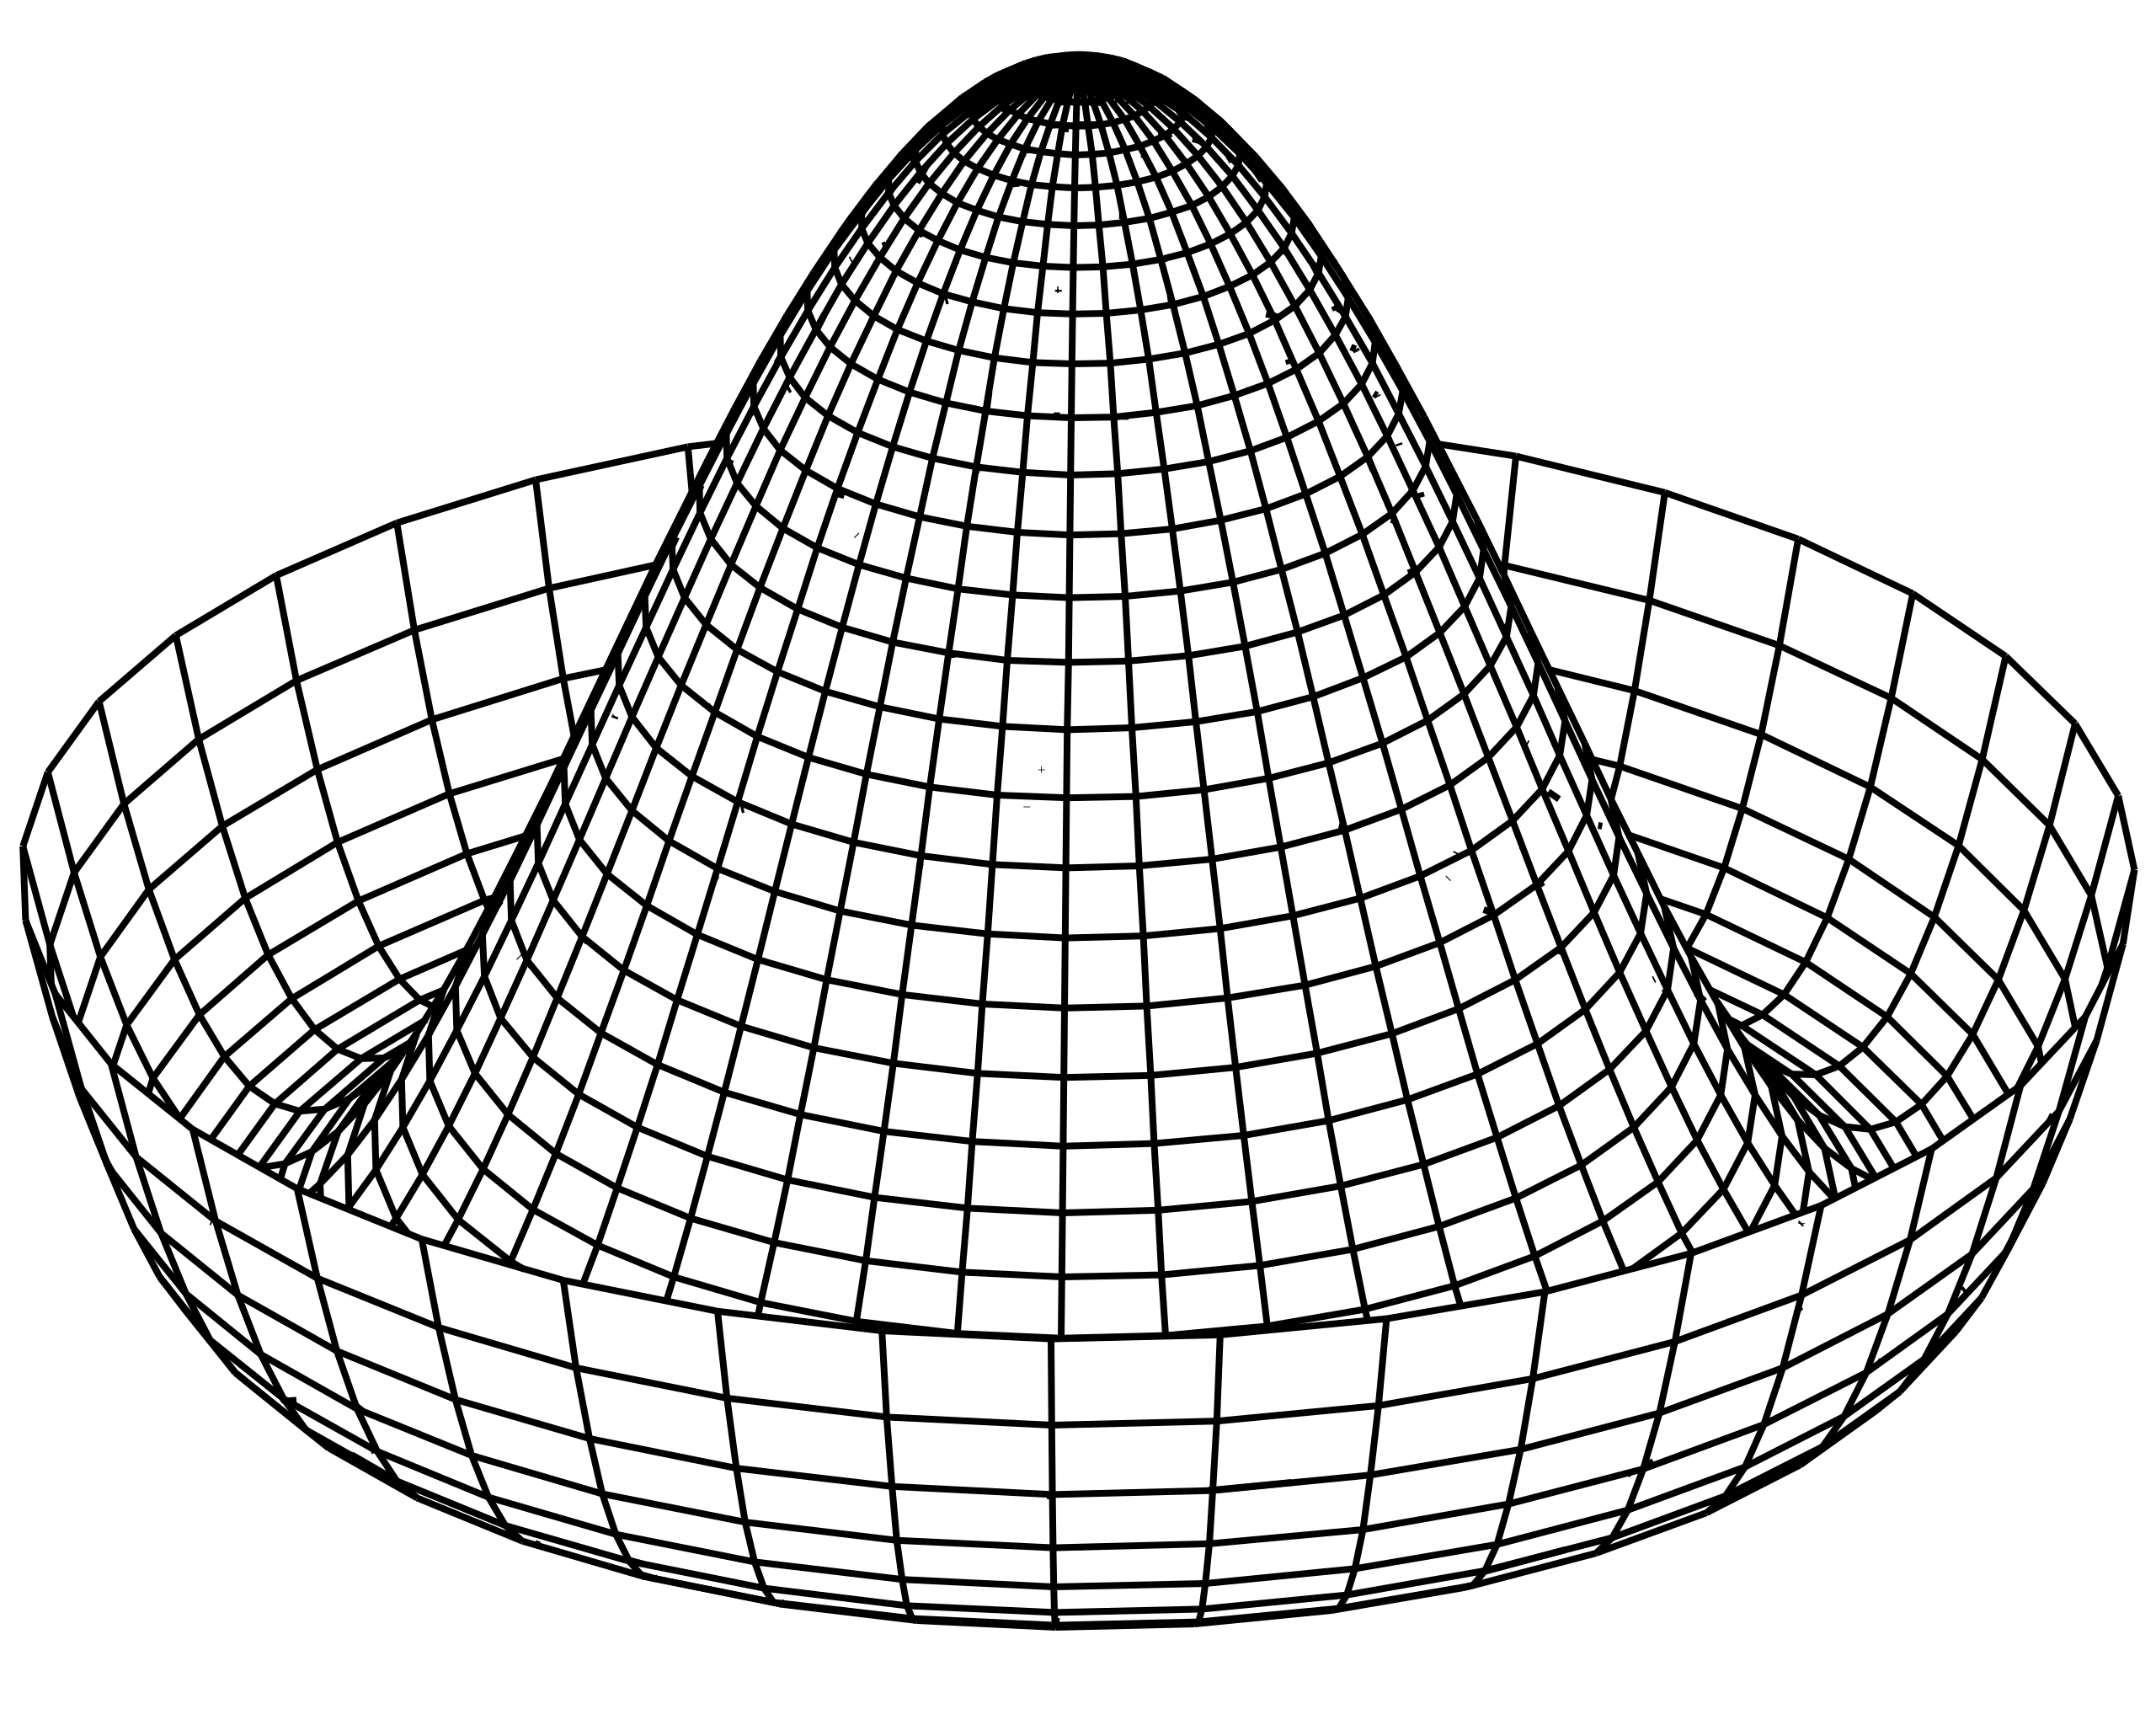
\includegraphics[width=0.5\textwidth]{figures/mexican_hat.png}
\caption{Visualization of $V(\phi)$ as the so-called ``Mexican hat'' potential.}
\label{fig:mexican_hat}
\end{figure}


Undertaking a unitary gauge transformation in SU(2), $\phi^+$ vanishes and $\phi^0$ remains as a physical scalar field.
Expanding this scalar field around the minimum of the potential in Equation~\ref{eq:higgsV}, $\phi^0 \rightarrow \frac{v+H(x)}{\sqrt{2}}$,
where $H(x)$ is a scalar at spacetime position $x$ with expected value 0.

Symmetry breaking alters the terms $\mathcal{L}_\mathrm{\phi}$ and $\mathcal{L}_\mathrm{Yukawa}$ in Equation~\ref{eq:EWpreSSB}, leaving the others unchanged. In a Lagrangian density, the kinetic and potential terms for such a scalar field $\phi$ are
\begin{equation}
\mathcal{L}_\phi = (D_\mu\phi)^\dagger(D^\mu\phi) - V(\phi) \label{eq:Lphi}
\end{equation}
Let us expand Equation~\ref{eq:Lphi} for the $\phi$-field using the previously defined $D_\mu$:
\begin{equation}
\begin{split}
%\mathcal{L}_\mathrm{Yukawa}  & = \sum_f -G_f \bar{f} f (v+H) \\
\mathcal{L}_\mathrm{\phi} & = \frac{1}{2} (\partial^\mu H) (\partial_\mu H) - \lambda\left[ v^2H^2 + vH^3 + \frac{1}{4}H^4\right] \\
& + \frac{1}{8} \left| g \hat{T}^1 A^1_\mu + g \hat{T}^2 A^2_\mu + g \hat{T}^3 A^3_\mu + g' Y B_\mu \right|^2 (v+H)^2
\end{split}
\end{equation}
Noting that $(\hat{T}^1 \pm i \hat{T}^2)/2 \equiv \hat{T}^\pm$ are the raising and lowering operators 
for the third component of weak isospin in the SU(2) symmetry,
and the charge operator $\hat{Q} = \hat{T}^3 - \hat{Y}$,
the last term in $\mathcal{L}_\mathrm{\phi}$ simplifies:
\begin{equation}
\mathcal{L}_\mathrm{\phi} = ... + \frac{1}{8}\left[ g^2(A^1_\mu)^2 + g^2(A^2_\mu)^2  + \left( gA^3_\mu + g' B_\mu \right)^2 \right] (v+H)^2
\end{equation}
If we define a weak angle $\theta_W = \mathrm{arctan}\frac{g'}{g}$, 
we view $gA^3_\mu + g' B_\mu$ as the $A^3$ and B bosons being rotated into two other bosons. 
These will be the massive Z boson and the massless $\gamma$ boson, also known as the photon \cite{Weinberg1967}.
Meanwhile, we can view the $A^1$ and $A^2$ bosons combining to give the charged $W^\pm$ bosons:
\begin{equation}
W^\pm = \frac{A^1 \mp iA^2}{\sqrt{2}} \label{eq:WpmA12}
\end{equation}
For completeness, let us rewrite the electroweak gauge covariant derivative in terms of the physical bosons.
The Z boson is represented by the gauge field $Z_\mu$ and the photon is represented by the gauge field $A_\mu$ without a superscript.
\begin{equation}
\label{eq:covariant_derivative}
D_\mu^\mathrm{EW} = \partial_\mu - \frac{ig}{\sqrt{2}} (W_\mu^+ \hat{T}^+ + W_\mu^- \hat{T}^-) - \frac{ig}{\mathrm{cos}\:\theta_W} Z_\mu( \hat{T}^3 - \mathrm{sin}^2 \: \theta_W \: \hat{Q}) - ie A_\mu \hat{Q}
\end{equation}
We can now rewrite $\mathcal{L}_\mathrm{\phi}$ from before, in terms of the physical W and Z bosons:
\begin{equation}
\label{eq:LhiggsWZ}
\begin{split}
\mathcal{L}_\mathrm{\phi} & = \frac{1}{2} (\partial^\mu H) (\partial_\mu H) - \lambda\left[ v^2H^2 + vH^3 + \frac{1}{4}H^4\right] \\
& + \left[ \frac{g^2}{4} W^+_\mu W^{{-}\mu}  + \frac{g^2}{8\:\mathrm{cos}^2\:\theta_W} Z_\mu Z^\mu \right](v+H)^2   \\
\end{split}
\end{equation}
From this expression, we can extract expressions for the W and Z bosons' masses at leading-order:
\begin{equation}
\label{eq:WZmass}
m_W = \frac{v g}{2},\:\:\:\:m_Z = \frac{vg}{2\:\mathrm{cos}\:\theta_W}
\end{equation}
Lastly, let us we reframe Equation~\ref{eq:EWpreSSB} in terms of the physical gauge bosons.
The antisymmetric photon, Z, and W field strength tensors $A_{\mu\nu}$, $Z_{\mu\nu}$, $W^{\pm}_{\mu\nu}$ are provided as
\begin{equation}
\begin{split}
A_{\mu\nu} &= \partial_\mu A_\nu - \partial_\nu A_\mu \\
Z_{\mu\nu} &= \partial_\mu Z_\nu - \partial_\nu Z_\mu \\
(\vec{\mathbf{W}}^{+}_{\mu\nu})_a &= \partial_\mu (\vec{\mathbf{W}}^{+}_\nu)_a - \partial_\nu (\vec{\mathbf{W}}^{+}_\mu)_a - ig\varepsilon_{abc}(\vec{\mathbf{W}}^{+}_\mu)_b (\vec{\mathbf{W}}^{+}_\nu)_c \\
\vec{\mathbf{W}}^{-}_{\mu\nu} &= (\vec{\mathbf{W}}^{+}_{\mu\nu})^\dagger
\end{split}
\end{equation}
where the vector notation indicates components in three-dimensional weak isospin space.
Einstein summation convention is used and $\varepsilon$ is the antisymmetric Levi-Civita symbol.

Finally, we can write down the full EW Lagrangian density after symmetry breaking. 
As before, $\mathcal{L}_\mathrm{EW} = \mathcal{L}_\mathrm{Gauge} + \mathcal{L}_\mathrm{Fermion} + \mathcal{L}_\mathrm{\phi} + \mathcal{L}_\mathrm{Yukawa}$. 
The $\mathcal{L}_\mathrm{Gauge}$ term contains the gauge field tensor dynamic terms, the triple-gauge couplings, and the quartic-gauge couplings:
\begin{equation} 
\begin{split}
\label{eq:L_Gauge}
\mathcal{L}_\mathrm{Gauge} & = -\frac{1}{4} \termLB A^{\mu\nu} A_{\mu\nu} + 2  W^+_{\mu\nu} W^{{-}\mu\nu} + Z_{\mu\nu} Z^{\mu\nu} \termRB  \\ 
 & - ig \termLB (W^+_{\mu\nu} W^{{-}\mu} - W^{+\mu} W^{{-}}_{\mu\nu})(A^\nu\mathrm{sin}\:\theta_W - Z^\nu \mathrm{cos}\:\theta_W)  \\
 & \qquad\qquad\qquad\qquad\qquad\qquad + W^{{-}}_{\nu} W^+_{\mu} (A^{\mu\nu} \mathrm{sin}\:\theta_W - Z^{\mu\nu} \mathrm{cos} \theta_W ) \termRB  \\
 & + \frac{g^2}{4} \termLB {-}\big( 2 W^+_\mu W^{{-}\mu} + (A_\mu \mathrm{sin}\:\theta_W - Z_\mu \mathrm{cos}\:\theta_W)^2 \big)^2 \\
 & \:\: + \big( W_\mu^+ W_\nu^{{-}} + W_\nu^+ W_\mu^{{-}} + (A_\mu \mathrm{sin}\:\theta_W - Z_\mu \mathrm{cos}\:\theta_W)(A_\nu\mathrm{sin}\:\theta_W - Z_\nu \mathrm{cos}\:\theta_W)\big)^2 \termRB
\end{split}
\end{equation}
The allowed gauge self-coupling vertices are pictured in Figures~\ref{fig:3GC} and~\ref{fig:4GC}.

The $\mathcal{L}_\mathrm{Fermion}$ term contains the interaction between the gauge bosons and the fermions, in the neutral current and the charged current:
\begin{equation}
\begin{split}
\label{eq:L_Fermion}
\mathcal{L}_\mathrm{Fermion} & = \termLB \frac{g}{\mathrm{cos}\:\theta_W} \big(J_\mu^\mathrm{3} - \mathrm{sin}^2\:\theta_W J_\mu^\mathrm{EM} \big) Z^\mu + eJ_\mu^\mathrm{EM} A^\mu \termRB \\
& - \frac{g}{\sqrt{2}} \termLB \big( \bar{u}_i \gamma^\mu \frac{1-\gamma^5}{2} V_{ij} d_j + \bar{\nu}_i \gamma^\mu \frac{1-\gamma^5}{2} e_i \big) W_\mu^+ + \mathrm{h.c.} \termRB
\end{split}
\end{equation}

The electromagnetic current is defined as $J^\mathrm{EM}_\mu \equiv \sum_f q_f \bar{f} \gamma_\mu f$ , with the bilinear covariant $\gamma_\mu$ representing the vector spin-1 coupling.
The weak neutral current is defined as $J^\mathrm{3}_\mu \equiv \sum_f T^3_f \bar{f} \gamma_\mu \frac{1-\gamma^5}{2} f$,
with the bilinear covariant representing the infamous ``vector minus axial'' spin-1 coupling.
The matrix $V_{ij}$ is the CKM matrix.

%This model is renormalizable

%\mathcal{L}_\mathrm{Fermion} & = \termLB \big( e A^\mu \sum_f q_f \bar{f} \gamma_\mu f \big) + \big( \frac{gZ^\mu}{\mathrm{cos}\:\theta_W}( \big)\termRB
%\mathcal{L}_\mathrm{Fermion} & = \sum_{f} \bar{f} i \gamma^\mu \partial_\mu - m_f) f \nonumber \\ 
%\mathcal{L}_\mathrm{\phi}    & = |D_\mu \phi|^2 - \lambda \left( |\phi|^2 - \frac{1}{2} v^2 \right)^2 \nonumber \\
%\mathcal{L}_\mathrm{Yukawa}  & = {-} \sum_f \frac{gm_f}{2m_W} \bar{f} f H \nonumber
%\end{align}
\begin{figure}[!hbt] % 3GC
 \centering
 \begin{tikzpicture} % WWZ
  \begin{feynman}
   \vertex (a2) {\(\boldsymbol{\W^\pm}\)};
   \vertex [right= 1.5cm of a2] (b1);
   \vertex [right= 1.1cm of b1] (c1);
   \vertex [above= 0.9cm of c1] (c2) {\(\boldsymbol{\Z}\)};
   \vertex [below= 0.9cm of c1] (c3) {\(\boldsymbol{\W^\pm}\)};
   
   \diagram* {
    (a2) -- [boson, very thick] (b1),
    (b1) -- [boson, very thick] (c2),
    (b1) -- [boson, very thick] (c3),
   };
  \end{feynman}
 \end{tikzpicture} \hspace{0.5cm}
 \begin{tikzpicture} % WWy
  \begin{feynman}
   \vertex (a2) {\(\boldsymbol{\W^\pm}\)};
   \vertex [right= 1.5cm of a2] (b1);
   \vertex [right= 1.1cm of b1] (c1);
   \vertex [above= 0.9cm of c1] (c2) {\(\boldsymbol{\gamma}\)};
   \vertex [below= 0.9cm of c1] (c3) {\(\boldsymbol{\W^\pm}\)};
   
   \diagram* {
    (a2) -- [boson, very thick] (b1),
    (b1) -- [boson, very thick] (c2),
    (b1) -- [boson, very thick] (c3),
   };
  \end{feynman}
 \end{tikzpicture} 
 \caption{Triple gauge boson vertices in the electroweak theory.} \label{fig:3GC}
\end{figure}

\begin{figure}[!hbt] % 4GC
 \centering
 \begin{tikzpicture} % WWWW
  \begin{feynman}
   \vertex (a1);
   \vertex [above= 0.8cm of a1] (a2) {\(\boldsymbol{\W}\)};
   \vertex [below= 0.8cm of a1] (a3) {\(\boldsymbol{\W}\)};
   \vertex [right= 1.2cm of a1] (b1);
   \vertex [right= 1.2cm of b1] (c1);
   \vertex [above= 0.8cm of c1] (c2) {\(\boldsymbol{\W}\)};
   \vertex [below= 0.8cm of c1] (c3) {\(\boldsymbol{\W}\)};
   
   \diagram* {
    (a2) -- [boson, very thick] (b1),
    (a3) -- [boson, very thick] (b1),
    (b1) -- [boson, very thick] (c2),
    (b1) -- [boson, very thick] (c3),
   };
  \end{feynman}
 \end{tikzpicture} \hspace{0.5cm}
 \begin{tikzpicture} % WWyy
  \begin{feynman}
   \vertex (a1);
   \vertex [above= 0.8cm of a1] (a2) {\(\boldsymbol{\W}\)};
   \vertex [below= 0.8cm of a1] (a3) {\(\boldsymbol{\W}\)};
   \vertex [right= 1.2cm of a1] (b1);
   \vertex [right= 1.2cm of b1] (c1);
   \vertex [above= 0.8cm of c1] (c2) {\(\boldsymbol{\gamma}\)};
   \vertex [below= 0.8cm of c1] (c3) {\(\boldsymbol{\gamma}\)};
   
   \diagram* {
    (a2) -- [boson, very thick] (b1),
    (a3) -- [boson, very thick] (b1),
    (b1) -- [boson, very thick] (c2),
    (b1) -- [boson, very thick] (c3),
   };
  \end{feynman}
 \end{tikzpicture} \hspace{0.5cm}
 \begin{tikzpicture} % WWyZ
  \begin{feynman}
   \vertex (a1);
   \vertex [above= 0.8cm of a1] (a2) {\(\boldsymbol{\W}\)};
   \vertex [below= 0.8cm of a1] (a3) {\(\boldsymbol{\W}\)};
   \vertex [right= 1.2cm of a1] (b1);
   \vertex [right= 1.2cm of b1] (c1);
   \vertex [above= 0.8cm of c1] (c2) {\(\boldsymbol{\gamma}\)};
   \vertex [below= 0.8cm of c1] (c3) {\(\boldsymbol{\Z}\)};
   
   \diagram* {
    (a2) -- [boson, very thick] (b1),
    (a3) -- [boson, very thick] (b1),
    (b1) -- [boson, very thick] (c2),
    (b1) -- [boson, very thick] (c3),
   };
  \end{feynman}
 \end{tikzpicture} \hspace{0.5cm}
 \begin{tikzpicture} % WWZZ
  \begin{feynman}
   \vertex (a1);
   \vertex [above= 0.8cm of a1] (a2) {\(\boldsymbol{\W}\)};
   \vertex [below= 0.8cm of a1] (a3) {\(\boldsymbol{\W}\)};
   \vertex [right= 1.2cm of a1] (b1);
   \vertex [right= 1.2cm of b1] (c1);
   \vertex [above= 0.8cm of c1] (c2) {\(\boldsymbol{\Z}\)};
   \vertex [below= 0.8cm of c1] (c3) {\(\boldsymbol{\Z}\)};
   
   \diagram* {
    (a2) -- [boson, very thick] (b1),
    (a3) -- [boson, very thick] (b1),
    (b1) -- [boson, very thick] (c2),
    (b1) -- [boson, very thick] (c3),
   };
  \end{feynman}
 \end{tikzpicture}
 \caption{Non-Abelian quartic gauge couplings in the electroweak theory.} \label{fig:4GC}
\end{figure}

\subsection{The Higgs boson}

Let us look at the second term of Equation~\ref{eq:LhiggsWZ}.
The portion $-\lambda v^2 H^2 $ suggests to us we can identify the quantum of the $H$-field as a physical boson with mass $m_H = \sqrt{2v^2\lambda}$.
We will call this quantum the Higgs boson, and the field, the Higgs field.

The $\mathcal{L}_\mathrm{\phi}$ term from the electroweak Lagrangian density can be expanded to find the Higgs couplings to itself and the other gauge bosons, in particular to the Z boson which is relevant to this work:

\begin{equation}
\begin{split}
\label{eq:L_phi}
\mathcal{L}_\mathrm{\phi} & = \termLB \frac{1}{2} (\partial^\mu H) (\partial_\mu H) - \frac{1}{2}m_H^2 H^2 \termRB - \termLB \frac{gm_H^2}{4m_W} H^3 + \frac{g^2m_H^2}{32m_W^2}H^4 \termRB \\
& + \termLB \left( W_\mu^+ W^{{-}\mu} + \frac{1}{2\mathrm{cos}^2\:\theta_W} Z_\mu Z^\mu \right) \left( gm_WH+\frac{g^2}{4}H^2 \right) \termRB
\end{split}
\end{equation}

Meanwhile, the $\mathcal{L}_\mathrm{Yukawa}$ term from the Lagrangian density becomes
\begin{equation}
\label{L_Yukawa}
\mathcal{L}_\mathrm{Yukawa} = {-} \sum_f \frac{gm_f}{2m_W} \bar{f}fH
\end{equation}
It provides for the Higgs boson to interact with and decay into fermions,
more likely for massive fermions.
The fermion mass $m_f$ truly arises from the coupling to the Higgs field, and not vice versa.

\begin{figure}[!hbt] % Higgs couplings
 \centering
\begin{tikzpicture} % VVH
  \begin{feynman}
   \vertex (a2) {\(\boldsymbol{\mathrm{V}}\)};
   \vertex [right= 1.3cm of a2] (b1);
   \vertex [right= 1.1cm of b1] (c1);
   \vertex [above= 0.9cm of c1] (c2) {\(\boldsymbol{\Hi}\)};
   \vertex [below= 0.9cm of c1] (c3) {\(\boldsymbol{\mathrm{V}}\)};
   
   \diagram* {
    (a2) -- [boson, very thick] (b1),
    (b1) -- [scalar, very thick] (c2),
    (b1) -- [boson, very thick] (c3),
   };
  \end{feynman}
 \end{tikzpicture} \hspace{0.5cm}
 \begin{tikzpicture} % Hff
  \begin{feynman}
   \vertex (a2) {\(\boldsymbol{f}\)};
   \vertex [right= 1.3cm of a2] (b1);
   \vertex [right= 1.1cm of b1] (c1);
   \vertex [above= 0.9cm of c1] (c2) {\(\boldsymbol{\Hi}\)};
   \vertex [below= 0.9cm of c1] (c3) {\(\boldsymbol{f}\)};
   
   \diagram* {
    (a2) -- [fermion, very thick] (b1),
    (b1) -- [scalar, very thick] (c2),
    (b1) -- [fermion, very thick] (c3),
   };
  \end{feynman}
 \end{tikzpicture} \hspace{0.5cm}
 \begin{tikzpicture} % HHH
  \begin{feynman}
   \vertex (a2) {\(\boldsymbol{\Hi}\)};
   \vertex [right= 1.3cm of a2] (b1);
   \vertex [right= 1.1cm of b1] (c1);
   \vertex [above= 0.9cm of c1] (c2) {\(\boldsymbol{\Hi}\)};
   \vertex [below= 0.9cm of c1] (c3) {\(\boldsymbol{\Hi}\)};
   
   \diagram* {
    (a2) -- [scalar, very thick] (b1),
    (b1) -- [scalar, very thick] (c2),
    (b1) -- [scalar, very thick] (c3),
   };
  \end{feynman}
 \end{tikzpicture} \hspace{0.5cm}
 \begin{tikzpicture} % HHHH
  \begin{feynman}
   \vertex (a1);
   \vertex [above= 0.8cm of a1] (a2) {\(\boldsymbol{\Hi}\)};
   \vertex [below= 0.8cm of a1] (a3) {\(\boldsymbol{\Hi}\)};
   \vertex [right= 1.2cm of a1] (b1);
   \vertex [right= 1.2cm of b1] (c1);
   \vertex [above= 0.8cm of c1] (c2) {\(\boldsymbol{\Hi}\)};
   \vertex [below= 0.8cm of c1] (c3) {\(\boldsymbol{\Hi}\)};
   
   \diagram* {
    (a2) -- [scalar, very thick] (b1),
    (a3) -- [scalar, very thick] (b1),
    (b1) -- [scalar, very thick] (c2),
    (b1) -- [scalar, very thick] (c3),
   };
  \end{feynman}
 \end{tikzpicture}
 \caption{Higgs boson couplings. V is a $\W^\pm$ or $\Z$ boson. $f$ are fermions.}
\end{figure}


\subsection{Strong nuclear force}

The strong nuclear force arises from the theory of the interactions of the quarks and the gluon, called quantum chromodynamics (QCD).
It is a non-Abelian gauge theory whose internal symmetry is represented by the group $\mathrm{SU}(3)$.

Quarks and gluons carry color charge, of which there are three kinds: red, green, and blue.
Negative color charge, carried by the antiquarks and the gluons, is usually represented by the prefix \textit{anti-}, e.g. anti-red.
In transmitting the strong force as its carrier, the gluon carries a positive color charge and a negative color charge.
A gluon could carry red and anti-blue color charge, for example.
There are eight such possible combinations, each of which is a different kind of gluon.
These eight gluons correspond to the eight generators of the $\mathrm{SU}(3)$ group.

Quarks are fermions, having intrinsic spin of 1/2. There are six quarks.
Each quark has a bare mass and an electric charge.
In bound states such as the proton, the quarks appear to weigh more.
This constituent quark mass is heavier because of the field of virtual quarks and gluons around the bare quarks.

\begin{table}[ht]
  \caption{The quarks. When significant, bare masses quote statistical followed by systematic uncertainty. \label{tab:quarks}}
  \begin{center} {\scriptsize
  \begin{tabular}{|p{1.5cm}|c|c|c|c|c|}
  \hline
  \bf{Quark} & \bf{Symbol} & \bf{Charge} & \bf{Isospin} & \bf{Bare mass} $\mathbf{[\MeV\:c^{-2}]}$ & \bf{Constituent mass} $\mathbf{[\MeV\:c^{-2}]}$ \\
  \hline
  Up         & $u$         & {+2/3}      & +1/2         & $2.3 \pm 0.7 \pm 0.5    $  & 336                               \\
  Down       & $d$         & {-1/3}      & -1/2         & $4.8 \pm 0.5 \pm 0.3    $  & 340                               \\
  Charm      & $c$         & {+2/3}      & 0            & $1275 \pm 25            $  & 1550                              \\
  Strange    & $s$         & {-2/3}      & 0            & $95 \pm 5               $  & 486                               \\
  Top        & $t$         & {+2/3}      & 0            & $173,210 \pm 510 \pm 710$  & 4730                              \\
  Bottom     & $b$         & {-1/3}      & 0            & $4180 \pm 30            $  & 177,000                           \\
  \hline
  \end{tabular}
  }
  \end{center}
\end{table}

The Dirac Lagrangian density which defines the interactions between quarks and gluons is
\begin{equation}
\mathcal{L}_\mathrm{QCD} = \sum_{\psi} \bar{\psi}_i \left( i \gamma^\mu ( \partial_\mu \delta_{ij} - i g_s G^a_\mu T^a_{ij}) - m_\psi \delta_{ij} \right) \psi_j - \frac{1}{4} G^a_{\mu\nu} G^{\mu\nu}_a
\end{equation}


\begin{itemize}
  \setlength\itemsep{0em}
  \item The index $a$ represents the eight gluons.
  \item The index $i$ represents the three colors.
  \item The indices $\mu,\nu$ represent spacetime.
  \item $g_s$ is the strong coupling constant, sometimes expressed as $\sqrt{4\pi\alpha_s}$ which varies as a function of energy scale (see Figure~\ref{fig:alphaS}.
  \item $\psi_i$ is a Dirac bi-spinor representing the field for a quark and its antiquark at spacetime point $x$. $\bar{\psi}_i$ is the adjoint as in section~\ref{qed}.
  \item $G^a_\mu$ is the $\mathrm{SU}(3)$ gauge field.
  \item $T^a_{ij}$ are the eight generators of the $\mathrm{SU}(3)$ group, also known as Gell-Mann matrices.
  \item Lastly, the symbol $G^a_{\mu\nu}$ is the gluon field strength tensor...
\end{itemize}
The gluon field strength tensor comes from the gluon fields, $\mathcal{A}^a_\mu(x)$, as such:
\begin{equation}
G^a_{\mu\nu} = \partial_\mu \mathcal{A}^a_\nu - \partial_\nu \mathcal{A}^a_\mu + g\:f^{abc} \mathcal{A}^b_\mu \mathcal{A}^c_\nu
\end{equation}
This quantum field theory permits the quark-quark-gluon vertex, the three-gluon vertex, and the four-gluon vertex.
\begin{figure}[!hbtp]
  \centering
    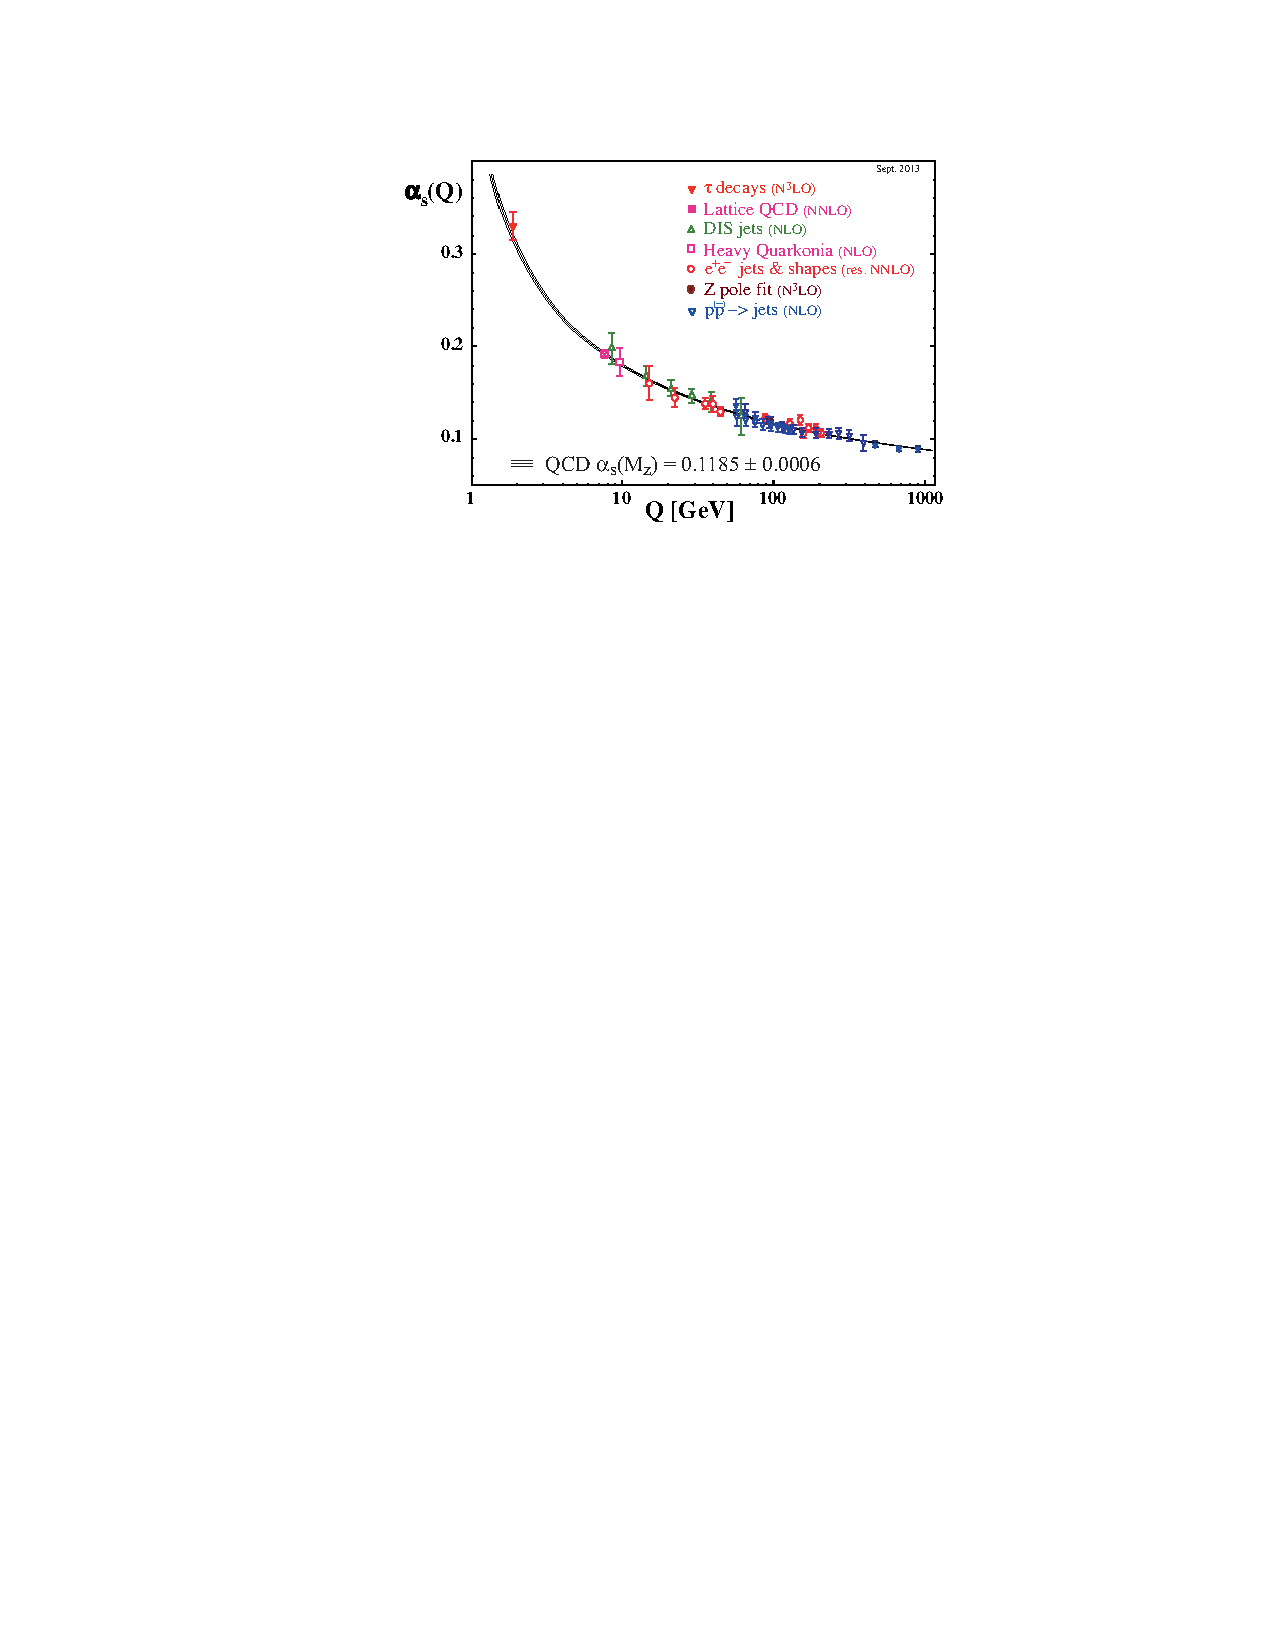
\includegraphics[width=0.80\textwidth]{figures/alphaS_running.pdf}
  \caption{The so-called ``running'' of $\alpha_S$ as the energy scale ~\cite{PhysRevD.98.030001}.} 
  \label{fig:alphaS}
\end{figure}

% Diagram
For experimental physics at the LHC, QCD is important even for studying electroweak processes.
Since we collide protons, the internal dynamics of the proton are an essential ingredient of Monte Carlo simulations.
The momentum fractions carried by the quarks and gluons are determined empirically as what are called the proton parton distribution functions.
Internal gluon loop corrections and the possibility of emitting extra gluons before or after the hard process can enhance the total cross section significantly for physics processes.
QCD activity resulting in charged hadrons may interfere with the ability to identify charged leptons in physics events of interest.
%Lastly, the hadronic radiation from the interaction point irradiates the detector components. This changes their material properties over time.
\clearpage
\section{Proton parton distribution functions}

The quarks and gluons inside a proton are collectively called partons.
The parton distribution functions (PDFs) $f_i(x,Q^2)$ give the probability of finding inside the proton a quark or gluon with momentum fraction $x$, in a hard process with momentum transfer $Q$.
According to the central feature of QCD, known as asymptotic freedom, the partonic interactions become asymptotically weak at short distances.
QCD can quantitatively predict the dependence of the PDFs on the energy scale, $Q^2$,
by way of the QCD evolution equations developed by Dokshitzer, Gribov, Lipatov, Altarelli, and Parisi (DGLAP).
These equations are valid in the regime where the strong coupling constant is small ($\alpha_S(Q^2) \ll 1$) so perturbative calculations are effective.
The DGLAP equations can make a statement about the $Q^2$ dependence, but the $x$ dependence is still unknown.
By the QCD factorization theorems, the PDFs can be related to the observable cross section of a
hard process by writing the cross section as a parton interaction convoluted with the PDFs \cite{Collins:1989gx}.
The parton interaction can be calculated using perturbative quantum field theory techniques.
The PDF shapes as a function of $x$ are not calculated theoretically and are instead determined empirically by experimental data.

\begin{figure}[hb]
  \centering
    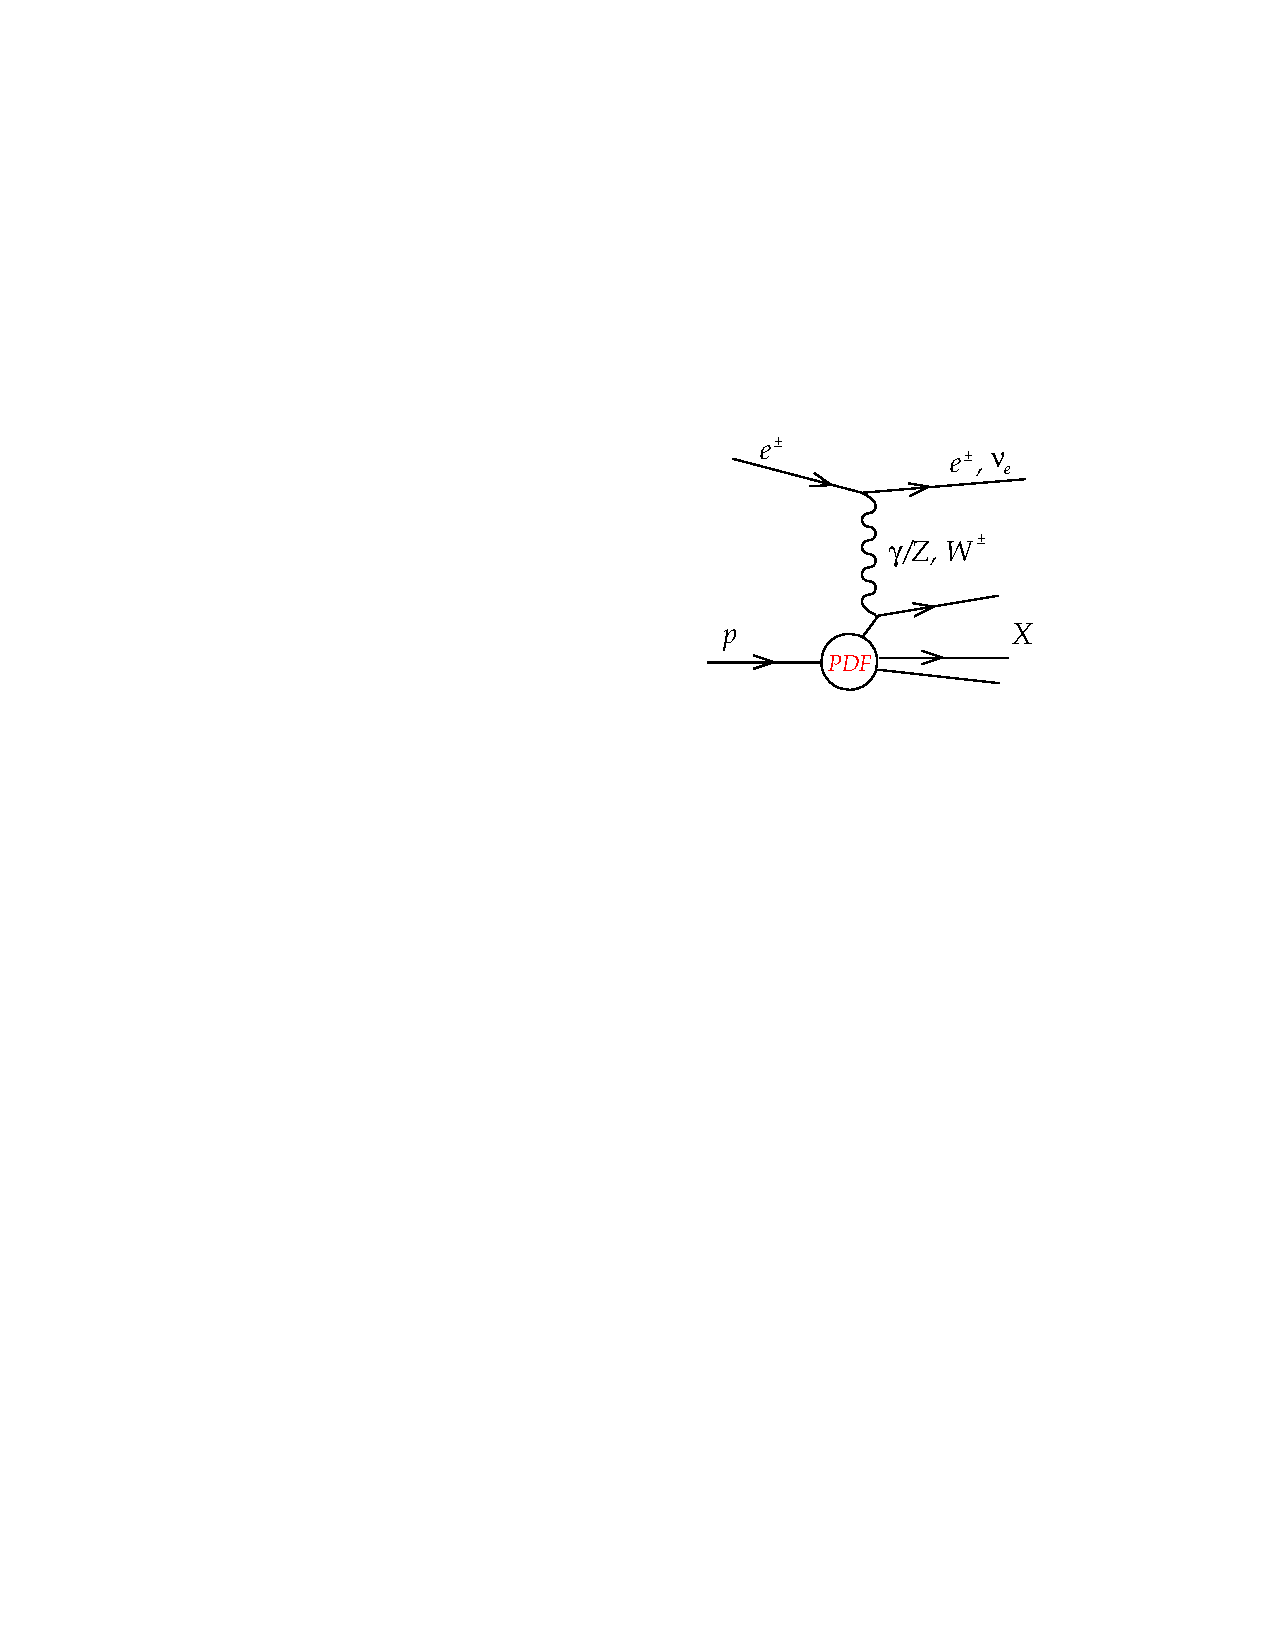
\includegraphics[width=0.50\textwidth]{figures/dis.pdf}
  \caption{Probing the PDFs with deep inelastic scattering. From \cite{Placakyte:2011az}.} 
  \label{fig:dis}
\end{figure}

The HERA experiment provided important data for the PDF determination by performing
deep inelastic scattering of electrons or positrons with protons, 
at center of mass energies of a few hundred \GeV.
Two different scattering processes can occur, called the neutral current and charged current; see Figure~\ref{fig:dis}.
In the charged current interaction, the cross sections of electron and positron on proton are sensitive to different quark PDFs.
%The neutral current $ep$ cross section can be expressed in terms of the structure functions $\tilde{F}$:
%\begin{equation}
%\frac{d^2 \sigma^{e^\pm p}_\mathrm{N.C.}}{dx\:dQ^2} = \frac{2 \pi \alpha^2}{xQ^4}\termLB Y_+ \tilde{F}^\pm_2 \mp Y_{-} x \tilde{F}^\pm_3 - y^2 \tilde{F}^\pm_L \termRB
%\end{equation}
%where $Y_\pm = 1 \pm (1-y^2)$ as a function of the inelasticity $y$.
%In general, $\tilde{F}_2$ dominates, $x\tilde{F^3}$ becomes important at higher $Q^2$,
%and $\tilde{F}_L$ only matters for significant $y$.
%The PDFs are directly related to these structure functions.
%Neglecting higher-order terms for the gluon density: $F_2$ is approximately the momentum sum of the 
%distributions of quarks and antiquarks ($F_2 \approx x\sum e_q^2 (q+\bar{q})$) 
%and $F_3$ is approximately their momentum difference ($xF_3 \approx x\sum 2e_qa_q(q-\bar{q}))$.
%
%The charged current $ep$ cross section can also be expressed in terms of structure functions.

In $p\bar{p}$ and $pp$ collisions at the Tevatron and LHC,
we can learn more about the proton PDFs through Standard Model precision measurements.
In particular, the Z boson differential cross section studied in this work contributes to the global fit of the quark distributions.
Meanwhile, ultraperipheral lead-lead heavy ion collisions are also an unconventional source of high energy photon probes which help us study the gluon distribution down to very small values of $x$ (see~\cite{Baltz:2007kq}).
Overall, the PDFs are an important quantity for simulating the Standard Model background in a search for new physics.
An example of the PDF set provided by the NNPDF collaboration at $Q=50 \GeV$ is shown in Figure~\ref{fig:pdfq50}.

\begin{figure}[hbtp]
  \centering
    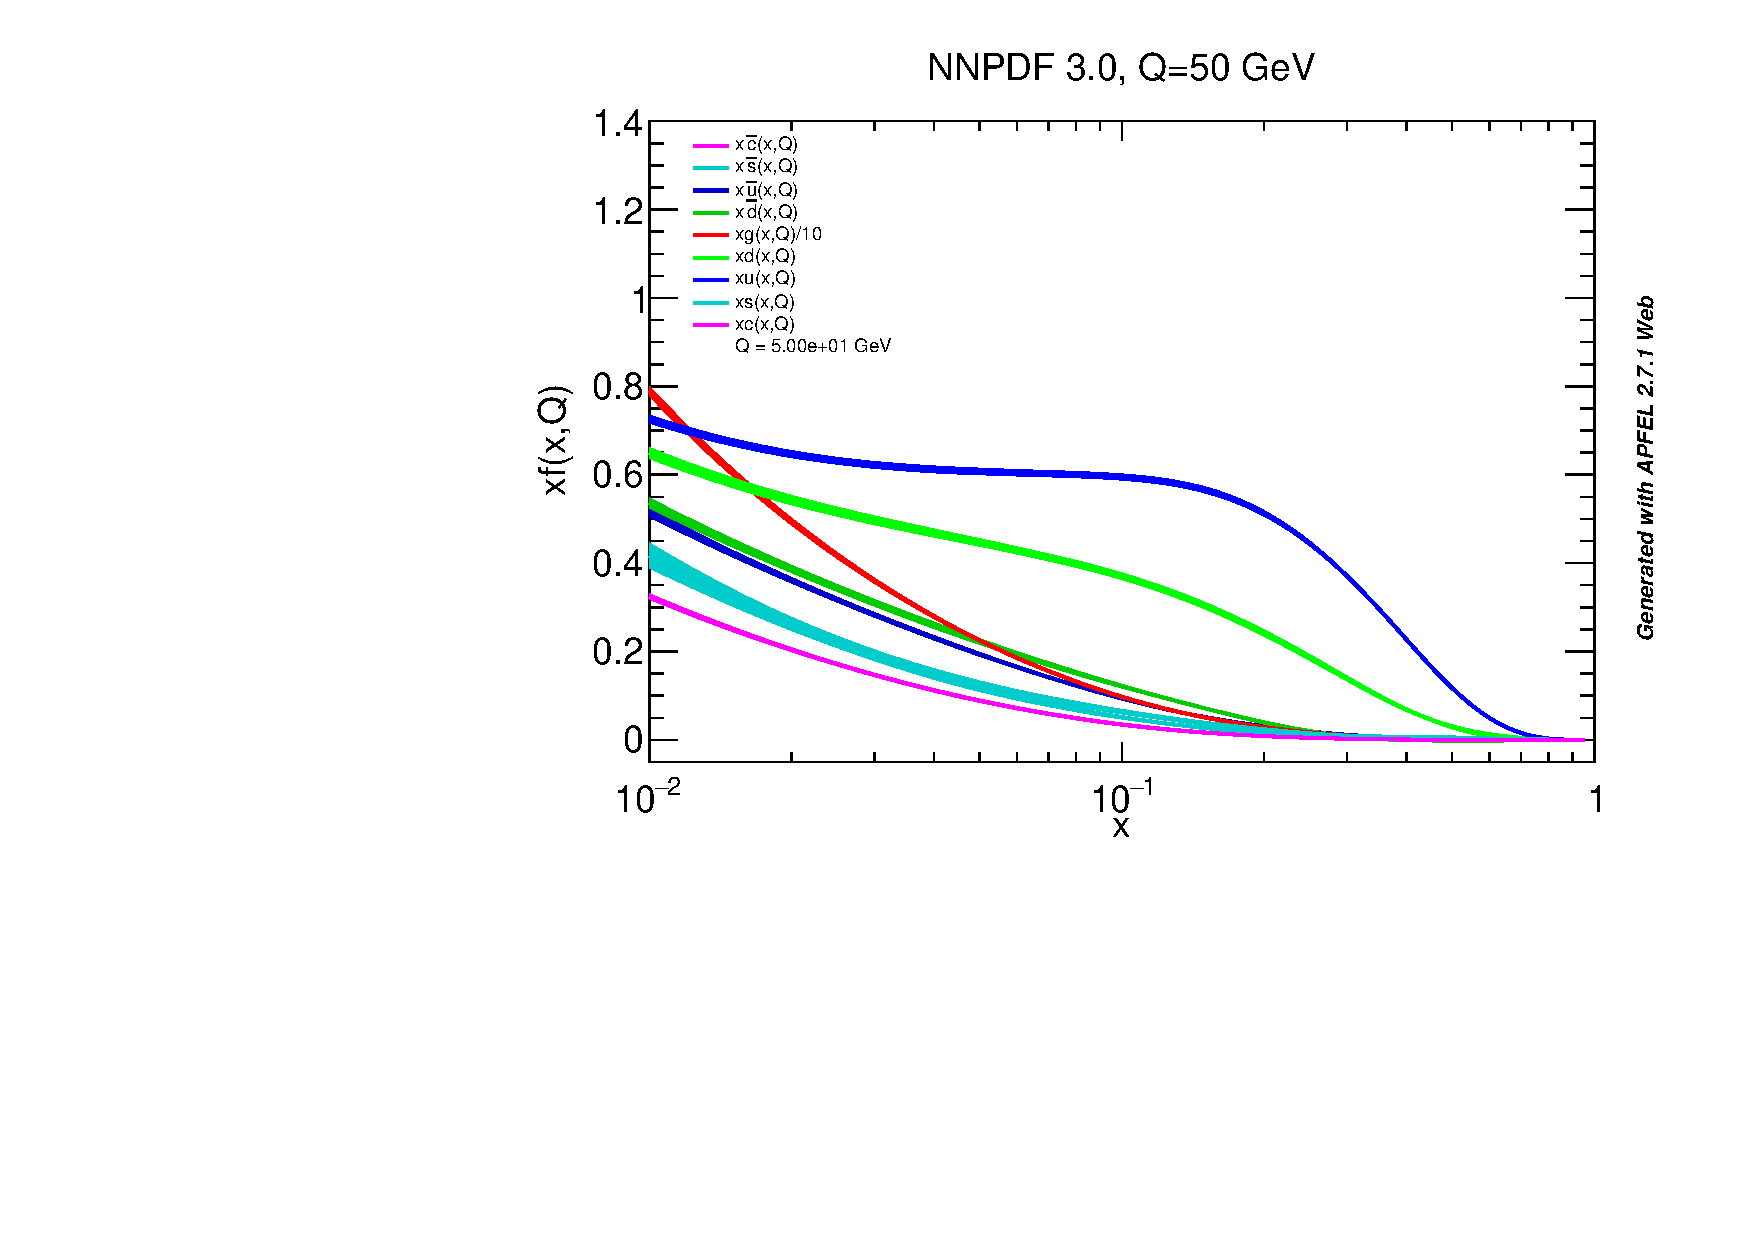
\includegraphics[width=0.90\textwidth]{figures/nnpdf30_115_Q50_v4.pdf}
  \caption{NNPDF 3.0 set at momentum transfer 50 \GeV. Presented in~\cite{nnpdf}.} 
  \label{fig:pdfq50}
\end{figure}

\section{New physics}
\label{sec:bsmtheory}
%In this work, we consider a scenario in which are produced a pair of charged leptons ($\ell^{+}\ell^{-}$, where $\ell=\Pe$ or $\Pgm$),
%consistent with the decay of a $\PZ$ boson, together with large missing transverse momentum ($\met$).

The study presented here considers one possible mechanism for producing weakly interacting massive particles at the LHC~\cite{Abercrombie:2015wmb}.
In this scenario, a $\PZ$ boson, produced in $pp$ collisions, recoils against a pair of DM particles, $\chi\overline\chi$.
The $\PZ$ boson subsequently decays into two charged leptons (electrons or muons), 
%producing a low-background dilepton signature, 
recoiling against $\met$ due to the undetected DM particles. 
We assume the final state dark matter particle $\chi$ is a Dirac fermion.

\begin{figure} % BSM models
 \centering
 \begin{tikzpicture} % ZH(inv)
  \begin{feynman}
   \vertex (q1) {\(\boldsymbol{\Pq}\)};
   \vertex [below= 3cm of q1] (q2) {\(\boldsymbol{\Paq}\)};
   \vertex [right= 1.6cm of q1] (a1);
   \vertex [below= 1.5cm of a1] (a2);
   \vertex [right= 1.6cm of a2] (b1);
   \vertex [right= 1.6cm of b1] (c1);
   \vertex [above= 1.3cm of c1] (c2);
   \vertex [below= 1.3cm of c1] (c3);
   \vertex [right= 1cm of c2] (d1);
   \vertex [right= 1cm of c3] (d2);
   \vertex [above= 0.3cm of d1] (f1) {\(\boldsymbol{\ell}\)};
   \vertex [below= 0.3cm of d1] (f2) {\(\boldsymbol{\bar{\ell}}\)};
   \vertex [above= 0.3cm of d2] (f3) {\(\boldsymbol{\chi}\)};
   \vertex [below= 0.3cm of d2] (f4) {\(\boldsymbol{\bar{\chi}}\)};
   
   \diagram* {
    (q1) -- [fermion, very thick] (a2),
    (q2) -- [anti fermion, very thick] (a2),
    (a2) -- [boson, very thick, edge label'=\(\boldsymbol{\Z^*}\)] (b1),
    (b1) -- [boson, very thick, edge label=\(\boldsymbol{\Z}\)] (c2),
    (b1) -- [scalar, very thick, edge label=\(\boldsymbol{\Hi}\)] (c3),
    (c2) -- [fermion, very thick] (f1),
    (c2) -- [anti fermion, very thick] (f2),
    (c3) -- [fermion, very thick] (f3),
    (c3) -- [anti fermion, very thick] (f4),
   };
  \end{feynman}
 \end{tikzpicture} \hspace{1cm}
 \begin{tikzpicture} % Simplified model spin-0 mediator
  \begin{feynman}
   \vertex (g1) {\(\boldsymbol{}\)};
   \vertex [below= 3.6cm of g1] (g2) {\(\boldsymbol{}\)};
   \vertex [right= 1.4cm of g1] (a1);
   \vertex [right= 1.4cm of g2] (a2);
   \vertex [below= 0.8cm of a1] (a3);
   \vertex [above= 0.8cm of a2] (a4);
   \vertex [right= 1.4cm of a3] (b1);
   \vertex [right= 1.4cm of a4] (b2);
   \vertex [right= 1.4cm of b1] (c1);
   \vertex [right= 1.4cm of b2] (c2);
   \vertex [right= 1cm of c1] (d1);
   \vertex [right= 1cm of c2] (d2);
   \vertex [above= 0.3cm of d1] (f1) {\(\boldsymbol{\ell}\)};
   \vertex [below= 0.3cm of d1] (f2) {\(\boldsymbol{\bar{\ell}}\)};
   \vertex [above= 0.3cm of d2] (f3) {\(\boldsymbol{\chi}\)};
   \vertex [below= 0.3cm of d2] (f4) {\(\boldsymbol{\bar{\chi}}\)};
   \vertex [below = 0.2cm of b2] (dm1) {\(\boldsymbol{g_\Pq}\)};
   \vertex [below = 0.2cm of c2] (dm2) {\(\boldsymbol{g_\mathrm{DM}}\)};
   
   \diagram* {
    (g1) -- [gluon, very thick] (a3),
    (g2) -- [gluon, very thick] (a4),
    (a3) -- [fermion, very thick, edge label'=\(\boldsymbol{\bar{\Top}}\)] (a4) -- [fermion, very thick, edge label=\(\boldsymbol{\Top}\)] (b2) -- [fermion, very thick, edge label=\(\boldsymbol{\bar{\Top}}\)] (b1) -- [fermion, very thick, edge label'=\(\boldsymbol{\Top}\)] (a3),
    (b1) -- [boson, very thick, edge label=\(\boldsymbol{\Z}\)] (c1),
    (b2) -- [scalar, very thick, edge label=\(\boldsymbol{\phi}\)] (c2),
    (c1) -- [fermion, very thick] (f1),
    (c1) -- [anti fermion, very thick] (f2),
    (c2) -- [fermion, very thick] (f3),
    (c2) -- [anti fermion, very thick] (f4),
   };
  \draw[fill=blue,line width=0pt] (b2) circle(1.5mm);
  \draw[fill=violet,line width=0pt] (c2) circle(1.5mm);
  \end{feynman}
 \end{tikzpicture} \vspace{1cm}
 
 \begin{tikzpicture} % Simplified model spin-1 mediator
  \begin{feynman}
   \vertex (q1) {\(\boldsymbol{\Pq}\)};
   \vertex [below= 3.6cm of q1] (q2) {\(\boldsymbol{\Paq}\)};
   \vertex [right= 2cm of q1] (a1);
   \vertex [right= 2cm of q2] (a2);
   \vertex [below= 0.8cm of a1] (a3);
   \vertex [above= 0.8cm of a2] (a4);
   \vertex [right= 2cm of a3] (b1);
   \vertex [right= 2cm of a4] (b2);
   \vertex [right= 1.5cm of b1] (c1);
   \vertex [right= 1.5cm of b2] (c2);
   \vertex [above= 0.3cm of c1] (f1) {\(\boldsymbol{\ell}\)};
   \vertex [below= 0.3cm of c1] (f2) {\(\boldsymbol{\bar{\ell}}\)};
   \vertex [below= 0.2cm of c2] (U) {\(\boldsymbol{\mathcal{U}/\mathcal{G}}\)};
   
   \diagram* {
    (q1) -- [fermion, very thick] (a3),
    (a3) -- [fermion, very thick] (a4),
    (q2) -- [anti fermion, very thick] (a4),
    (a3) -- [boson, very thick, edge label=\(\boldsymbol{\Z}\)] (b1),
    (a4) -- [ghost, very thick] (U),
    (b1) -- [fermion, very thick] (f1),
    (b1) -- [anti fermion, very thick] (f2),
   };
  \draw[fill=black,line width=0pt] (a4) circle(2.2mm);
  \draw[pattern=north east lines, pattern color=white] (a4) circle(2.2mm);
  \end{feynman}
 \end{tikzpicture} \hspace{1cm}  
 \begin{tikzpicture} % ADD/unparticles
  \begin{feynman}
   \vertex (q1) {\(\boldsymbol{\Pq}\)};
   \vertex [below= 3.6cm of q1] (q2) {\(\boldsymbol{\Paq}\)};
   \vertex [right= 2cm of q1] (a1);
   \vertex [right= 2cm of q2] (a2);
   \vertex [below= 0.8cm of a1] (a3);
   \vertex [above= 0.8cm of a2] (a4);
   \vertex [right= 2cm of a3] (b1);
   \vertex [right= 2cm of a4] (b2);
   \vertex [right= 1.5cm of b1] (c1);
   \vertex [right= 1.5cm of b2] (c2);
   \vertex [above= 0.3cm of c1] (f1) {\(\boldsymbol{\ell}\)};
   \vertex [below= 0.3cm of c1] (f2) {\(\boldsymbol{\bar{\ell}}\)};
   \vertex [above= 0.3cm of c2] (f3) {\(\boldsymbol{\chi}\)};
   \vertex [below= 0.3cm of c2] (f4) {\(\boldsymbol{\bar{\chi}}\)};
   \vertex [below = 0.2cm of a4] (dm1) {\(\boldsymbol{g_\Pq}\)};
   \vertex [below = 0.2cm of b2] (dm2) {\(\boldsymbol{g_\mathrm{DM}}\)};
   
   \diagram* {
    (q1) -- [fermion, very thick] (a3),
    (a3) -- [fermion, very thick] (a4),
    (q2) -- [anti fermion, very thick] (a4),
    (a3) -- [boson, very thick, edge label=\(\boldsymbol{\Z}\)] (b1),
    (a4) -- [boson, very thick, edge label=\(\boldsymbol{\mathcal{A}}\)] (b2),
    (b1) -- [fermion, very thick] (f1),
    (b1) -- [anti fermion, very thick] (f2),
    (b2) -- [fermion, very thick] (f3),
    (b2) -- [anti fermion, very thick] (f4),
   };
  \draw[fill=blue,line width=0pt] (a4) circle(1.5mm);
  \draw[fill=violet,line width=0pt] (b2) circle(1.5mm);
  \end{feynman}
 \end{tikzpicture}
 \caption{Some diagrams beyond the Standard Model in which are produced two charged leptons and missing energy. Clockwise from upper left: associated production of an invisible Higgs boson; gluon-induced production of a Z boson and a massive spin-0 dark matter mediator via top-quark loop; production of a Z boson and a massive spin-1 dark matter mediator; production of a Z boson in association with gravitons (ADD model) or unparticles.} \label{fig:BSMdiagrams}
\end{figure}

\subsection{Simplified models}
Four simplified models of DM production via an $s$-channel mediator exchange are considered.
In these models, the mediator has a spin of 1 (0) and vector or axial-vector (scalar or pseudoscalar) couplings to quarks and DM particles.
The free parameters of each model are the masses $m_{\rm med}$ and $m_{\rm DM}$ of the mediator and DM particle, respectively, as well as the coupling
constant $g_{\Pq}$ ($g_{\rm DM}$) between the mediator and the quarks (DM particles).
The vector coupling model is described with the following Lagrangian:

\begin{equation*}
\mathcal{L}_{\text{vector}} = g_{\rm DM} {Z'}_{\mu}\overline{\chi}\gamma^{\mu}\chi  + g_{\Pq} \sum_{\Pq} {Z'}_{\mu} \overline{\Pq}\gamma^{\mu}\Pq
\end{equation*}

\noindent where the spin-1 mediator is denoted as $\PZ'$ and the SM quark fields are referred to as \PQq and $\overline{\PQq}$.
The Lagrangian for an axial-vector coupling is obtained by making the replacement $\gamma^\mu\rightarrow\gamma^5\gamma^\mu$.
In the case of a spin-0 mediator $\phi$, the couplings between mediator and quarks are assumed to be Yukawa-like, with $g_{\Pq}$ acting as a 
multiplicative modifier for the SM Yukawa coupling ${y_{\Pq} = \sqrt{2}m_{\Pq}/v}$ (where $v = 246 \GeV$ is the SM Higgs field vacuum expectation value),
leading to the Lagrangian:

\begin{equation*}
\mathcal{L}_{\text{scalar}} = g_{\rm DM} {\phi}\overline{\chi}\chi  + g_{\Pq} \frac{\phi}{\sqrt{2}}\sum_{\Pq} y_{\Pq} \overline{\Pq}\Pq.
\end{equation*}

\noindent The Lagrangian with pseudoscalar couplings is obtained by inserting a factor of $i\gamma^5$ into each of the two terms (i.e., $\bar\chi\chi \to i\bar\chi\gamma^5\chi$ and $\bar \Pq \Pq \to i\bar \Pq\gamma^5 \Pq$). Example diagrams of DM production via spin-0 and spin-1 mediators are shown in Fig.~\ref{fig:BSMdiagrams} (upper right and lower right, respectively).

%\begin{figure}[!hbtp]
%  \centering
%    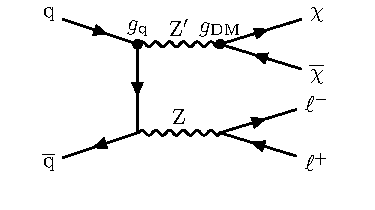
\includegraphics[width=0.45\textwidth]{figures/dmSimpFeynman.pdf}
%    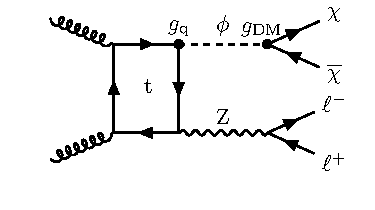
\includegraphics[width=0.45\textwidth]{figures/dmSimpFeynman_spin0.pdf}
%    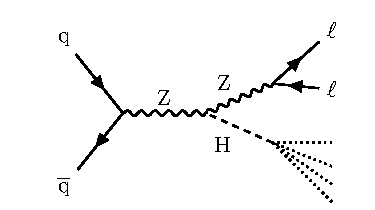
\includegraphics[width=0.45\textwidth]{figures/higgsInvisibleFeynman.pdf}
%    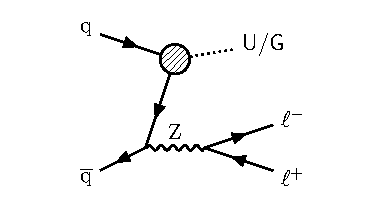
\includegraphics[width=0.45\textwidth]{figures/graph_UG.pdf}
%  \caption{Feynman diagrams illustrative of the processes beyond the SM considered in this paper:
%    (upper left)~DM production in a simplified model with a spin-1 mediator $\PZ'$;
%    (upper right)~DM production in a simplified model with a spin-0 mediator $\phi$;
%    (lower left)~production of a Higgs boson in association with Z boson with subsequent decay of the Higgs boson into invisible particles;
%    (lower right)~unparticle or graviton production. The diagrams were drawn using the {\sc TikZ-Feynman} package~\cite{Ellis:2016jkw}.
%  } 
%      \label{fig:Feynman}
%\end{figure}

\subsection{Invisible Higgs bosons}

A primary focus of the LHC physics program after the discovery of the Higgs boson ~\cite{AtlasPaperCombination,CMSPaperCombination} by
the ATLAS and CMS Collaborations is the study of the properties of this new particle. The observation of a sizable branching
fraction of the Higgs boson to invisible states~\cite{Ghosh:2012ep,Martin:1999qf,Bai:2011wz} would be a strong sign
of BSM physics.  Supersymmetric (SUSY) models embodying R-parity conservation contain a stable neutral lightest SUSY
particle (LSP), e.g., the lightest neutralino~\cite{Belanger:2001am}, leading to the possibility of decays of the Higgs boson into pairs of LSPs.
Certain models with extra spatial dimensions predict graviscalars that could mix with the
Higgs boson~\cite{Giudice:2000av}.  As a consequence, the Higgs boson could oscillate
to a graviscalar and disappear from the SM brane. The signature would be
equivalent to an invisible decay of the Higgs boson. There could also be contributions
from Higgs boson decays into graviscalars~\cite{Battaglia:2004js}.
Other ``Higgs portal'' models~\cite{Baek:2012se,Djouadi:2011aa,Djouadi:2012zc} construct
a generic connection between SM and DM particles via a Higgs boson mediator.
This work considers decays into invisible particles of an SM-like Higgs boson produced in association with a $\PZ$ boson, as shown in Fig.~\ref{fig:BSMdiagrams} (upper left).

\subsection{Extra dimensions}

A popular BSM paradigm considered here is the Arkani-Hamed--Dimopoulos--Dvali (ADD) model with large extra spatial dimensions~\cite{arkani98:hlz,arkani99:hlz,han99:hlz}, which
is motivated by the hierarchy problem, i.e., the disparity between the electroweak unification
scale ($M_\mathrm{EW} \sim 1\TeV$) and the Planck scale ($M_\mathrm{Pl} \sim 10^{16}\TeV$).
The Planck scale is the energy scale at which quantum effects of gravity become dominant and the Standard Model becomes unified with gravitation.
In the ADD model, the apparent Planck scale in four space-time dimensions
is given by $M_\mathrm{Pl}^2 \approx M_\mathrm{D}^{n+2}R^n$, where $M_\mathrm{D}$ is the true Planck scale of
the full $n$+4 dimensional space-time and $R$ is the compactification radius of the extra
dimensions.
The meaning of compactification is that the extra dimensions are finite or periodic in length.
In the limit of sufficiently high length scales or low energy scales, no fields depend on this extra dimension, so it reduces to a standard 4-dimensional space-time.
Assuming $M_\mathrm{D}$ is of the same order as $M_\mathrm{EW}$, the observed large value
of $M_\mathrm{Pl}$ points to an $R$ of order 1 mm to 1 fm for 2 to 7 extra dimensions.
The consequence of the large compactification scale is that the mass spectrum of the
Kaluza--Klein graviton states becomes nearly continuous, resulting in a broad $\PZ$ boson transverse momentum (\PT) spectrum.
Therefore, this model predicts graviton (\cPG) production via the process $\PQq\PAQq \rightarrow \PZ + \cPG$.
The graviton escapes detection, leading to the signature of a Z boson and missing energy (Fig.~\ref{fig:BSMdiagrams}, lower right).

\subsection{Unparticles}

The final BSM model considered in this work is the phenomenologically interesting concept of unparticles, which appear in the low-energy limit of conformal field theories.
In the Standard Model, only massless particles exhibit scale invariance.
Undertaking a scale transformation, all dimensional quantities are multipled by a rescaling factor
raised to the mass dimension. Thus, the massless particle's mass is unaffected.
Unparticles arise from massive BSM fields which scale with fractional dimensions ~\cite{Kang:2014cia,Rinaldi:2014gha,Cheng:1988zx}. 
In other words, the field's quantities are multiplied by fractional powers of the rescaling parameter, allowing for scale invariance.


In the high-energy regime, a scale invariant Banks--Zaks field with a nontrivial infrared fixed point is introduced~\cite{Banks:1981nn}.
The interaction between the SM and Banks--Zaks sectors is mediated by particles of large mass scale $M_{\textsf{U}}$, below which the interaction is suppressed and can be treated
via an effective field theory (EFT). The low-energy regime will include unparticles.
%, which have phase space factors equivalent to those of a noninteger
%number of ordinary particles
In this work, the emission of spin-0 unparticles from SM quarks is considered.
Because of the weakness of the unparticle interactions with the SM fields, the unparticle evades detection.
The EFT Lagrangian used to interpret the results is defined as follows:

\begin{equation*}
\mathcal{L}_{U}  = \frac{\lambda}{\LU^{\dU-1}} \mathcal{O}_{\textsf{U}} \overline{\PQq}\PQq,
\end{equation*}

\noindent where $\lambda$ represents the coupling between the SM and unparticle fields, \LU is the cutoff scale of the EFT, and \dU is the characteristic scaling dimension of the theory.
The unparticle operator is denoted as $\mathcal{O}_{\textsf{U}}$.
A representative Feynman diagram of the interaction is shown in Fig.~\ref{fig:BSMdiagrams} (lower right).



\chapter{Experimental apparatus}

The data studied in this work were collected at the Compact Muon Solenoid (CMS) Experiment.
The CMS detector is a multi-purpose apparatus which records the particle collisions
of the Large Hadron Collider.
It is installed about 100 meters underground close to the French village of Cessy,
between Lake Geneva and the Jura mountains.


\section{The Large Hadron Collider}

The LHC is a two-ring superconducting hadron accelerator \cite{lhcmachine}.
It is designed to collide counter-rotating proton beams with a center-of-mass energy of 14 TeV
and instantaneous luminosity of $10^{34}$ cm\textsuperscript{-2}s\textsuperscript{-1}.
In 2016, protons were collided at at center-of-mass energy of 13 TeV. 
The LHC has also collided lead ions with an energy of 2.8 TeV per nucleon and xenon ions with 2.72 TeV per nucleon.

First, hydrogen atoms are stripped of their protons with a large electric field.
They are accelerated to 450 GeV in the CERN LHC injector chain \cite{lhcinjector}.
The chain is as follows: Linac2 (50 MeV), Proton Synchotron Booster (1.4 GeV), Proton Synchotron (25 GeV), Super Proton Synchotron (450 GeV).
After the SPS, the protons are injected into the LHC's two separate rings in discrete proton bunches.
At the designed spacing of 25 nanoseconds between bunches, there are about 2800 proton bunches per beam.

The LHC achieves the final beam energy with 1232 dipole magnets, each 15 m in length with peak dipole field of 8.3 T.
The beam is focused using 492 quadrupole magnets of length 5-7 m.
These magnets are twin bore niobium-titanium superconducting electromagnets which operate at 1.9\textdegree~K.
The pipes for the counter-rotating beams are magnetically coupled and the magnets share the same cryostat.
Due to the necessity of very efficient heat transfer for prolonged periods, superfluid helium is used as a coolant.

The physics processes studied at the LHC are rare compared to the total proton-proton collision cross section.
A high beam intensity is needed to deliver them at a sufficient rate.
For a Gaussian beam distribution, the machine luminosity is
\begin{equation}
L = \frac{N_b^2 n_b f_\mathrm{rev} \gamma_r F}{4\pi\varepsilon_n \beta^*}
\end{equation}
where
\begin{itemize}
\item $N_b$ is the number of protons per bunch $\approx 10^{11}$
\item $n_b$ is the number of bunches per beam $\approx 2800$
\item $f_\mathrm{rev}$ is the revolution frequency 
\item $\gamma_r$ is the Lorentz factor,
\item $F$ is the reduction factor due to the geometric crossing angle
\item $\varepsilon_n$ is the transverse beam emittance normalized to the beam energy, describing the spread in position and momentum space
\item $\beta^*$ is the beta function at the interaction point, which alongside $\varepsilon_n$ determines the beam envelope
\end{itemize}

The LHC has 4 interaction points. The two general purpose, high luminosity experiments are ATLAS and CMS.
The LHCb experiment has only forward coverage and specializes in heavy flavor physics and spectroscopy.
The ALICE experiment studies heavy ion collisions.

In 2016, the LHC delivered around 36 inverse femtobarns worth of data which was recorded by CMS.

\begin{figure}[hbtp]
\centering
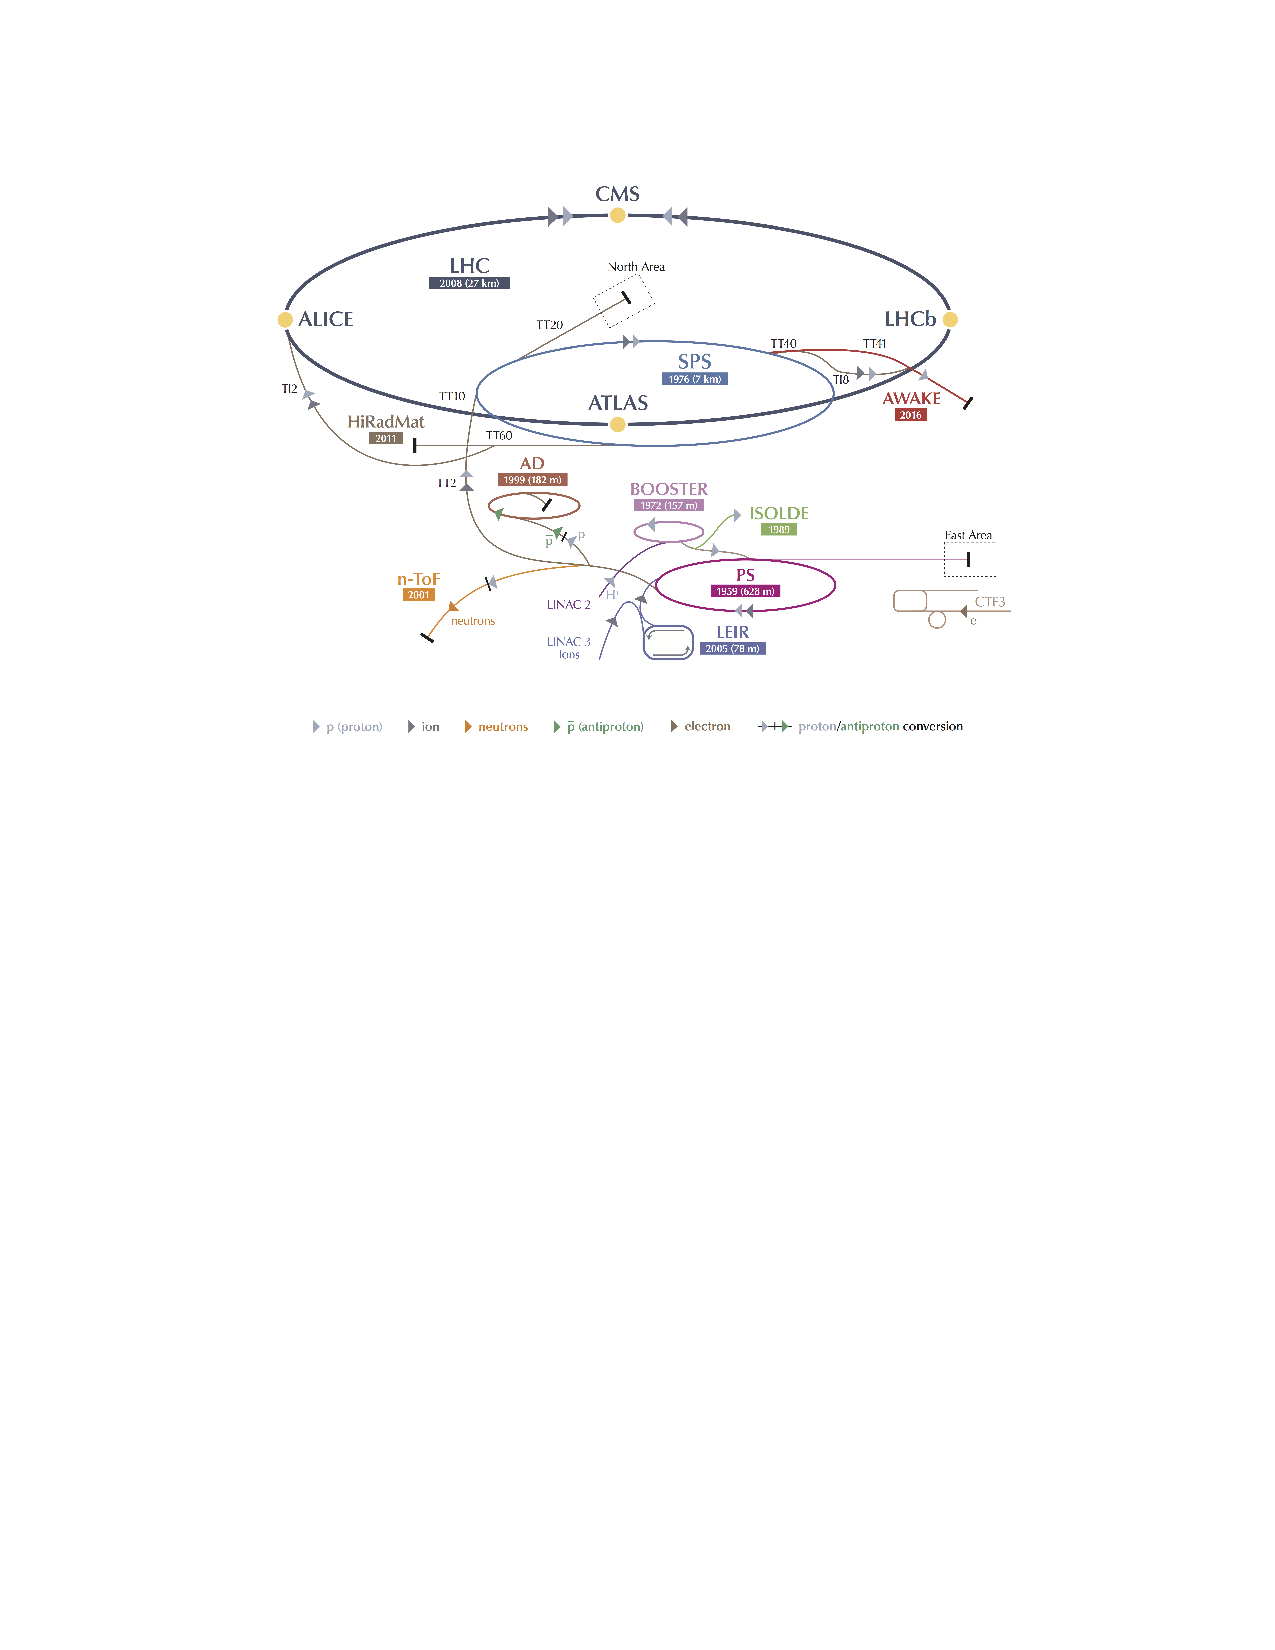
\includegraphics[width=0.9\textwidth]{figures/lhc_protons.pdf}
\caption{Schematic of the CERN accelerator complex.}
\label{fig:lhc}
\end{figure}


\section{The CMS detector}

CMS was designed with the following requirements in mind (in no particular order):
\begin{itemize}
\item Good muon identification and momentum resolution over a wide range of momenta and
angles, good dimuon mass resolution (1\% at 100 GeV), and the ability to determine unambiguously
the charge of muons with p < 1 TeV
\item Good charged-particle momentum resolution and reconstruction efficiency in the inner
tracker. Efficient triggering and offline tagging of $\tau$'s and b-jets, requiring pixel detectors
close to the interaction region
\item Good electromagnetic energy resolution, good diphoton and dielectron mass resolution (1\% at 100 GeV),
wide geometric coverage, ${\pi}^{0}$ meson rejection, and efficient photon and lepton
isolation at high luminosities
\item Good missing transverse energy and dijet mass resolution, requiring hadron calorimeters
with a large hermetic geometric coverage and with fine lateral segmentation
\end{itemize}

\begin{figure}[hb]
\centering
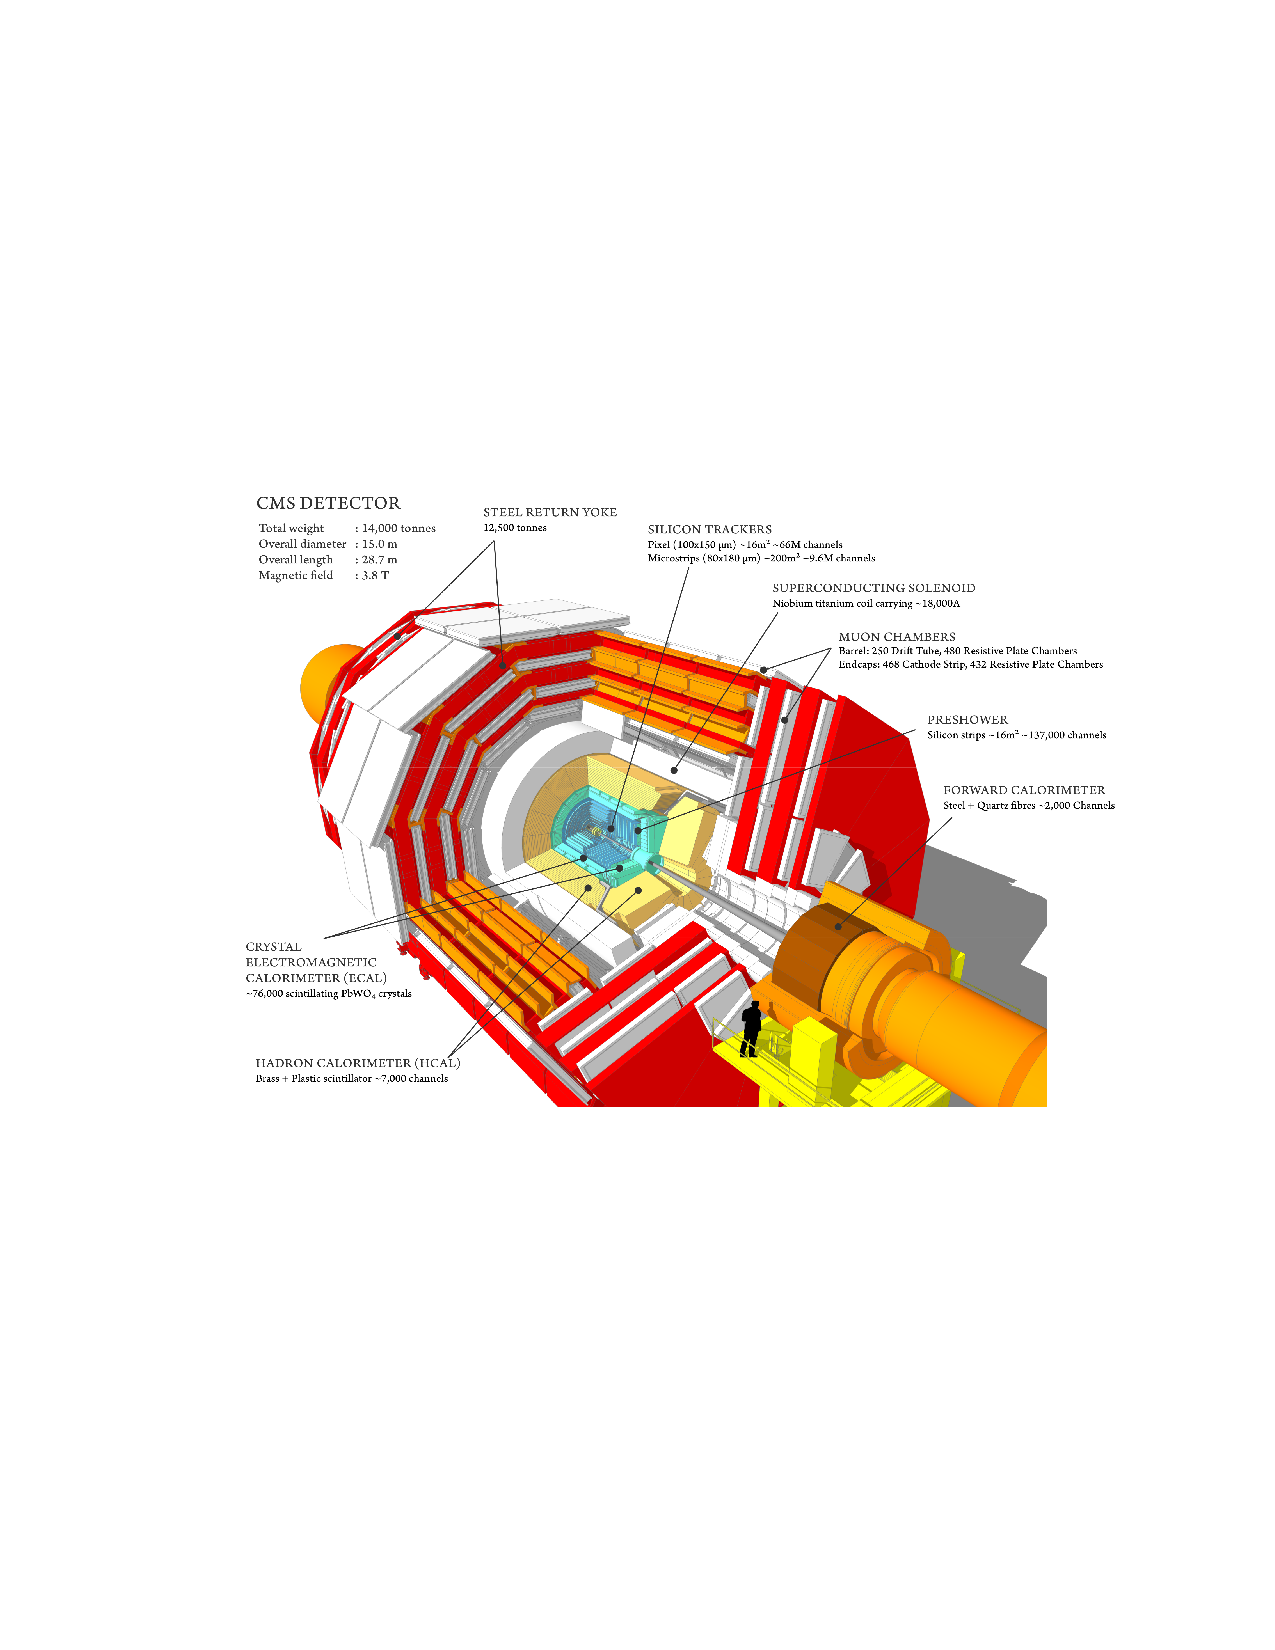
\includegraphics[width=0.95\textwidth]{figures/cms_detector.pdf}
\caption{Schematic of the CMS detector.}
\label{fig:cmsdetector}
\end{figure}

The central feature of the CMS apparatus is a superconducting solenoid of 6 m internal diameter, providing a magnetic field of 3.8 T.
Within the solenoid volume are a silicon pixel and strip tracker, a lead tungstate crystal electromagnetic calorimeter (ECAL), and a brass and scintillator hadron calorimeter (HCAL), each composed of a barrel and two endcap sections. 
Forward calorimeters extend the pseudorapidity coverage provided by the barrel and endcap detectors. 
Muons are detected in gas-ionization chambers embedded in the steel flux-return yoke outside the solenoid.

Events of interest are selected using a two-tiered trigger system~\cite{Khachatryan:2016bia}.
The first level, composed of custom hardware processors, uses information from the calorimeters and muon detectors to select events at a rate of around 100 kHz within a time interval of less than 4 $\mu$s.
The second level, known as the high-level trigger, consists of a farm of processors running a version of the full event reconstruction software optimized for fast processing, and reduces the event rate to around 1 kHz before data storage.

\subsubsection{Coordinate system}
To describe location, CMS uses a standard right-handed Cartesian coordinate system where 
the $x$ direction points to the center of the LHC ring, 
the $y$ direction points to the sky,
and the $z$ direction points in the counterclockwise beam direction at the interaction point.
This is used for locating interaction vertices and tracks' impact parameters with respect to those vertices.
However, this work will also frequently use a set of modified spherical coordinates $(r,\phi,\eta)$
which are conventional in particle physics.
Here, $r$ is the radial coordinate, $\phi$ is the azimuthal angle, and $\eta$ is the \textit{pseudorapidity}, given by
\begin{equation}
\eta  \equiv {-} \mathrm{ln}\:\mathrm{tan}\:\frac{\theta}{2} \implies \theta \equiv 2\:\mathrm{arctan} \left(e^{-\eta}\right)
\label{eq:eta}
\end{equation}
where $\theta$ is the polar angle. 
In these coordinates, the transverse momentum $p_T$ of a particle is related to its total momentum $|\vec{p}|$ and the hyperbolic secant of pseudorapidity as
\begin{equation}
p_T = |\vec{p}|~\mathrm{sech}~\eta
\end{equation}

A variable used to denote the angular separation between two objects in the detector is $\Delta R$,
which is defined as
\begin{equation}
\Delta R = \sqrt{(\phi_1-\phi_2)^2 + (\eta_1-\eta_2)^2}
\end{equation}

\subsection{Trackers}

The inner tracking system of CMS is designed to provide a precise and efficient measurement
of the trajectories of charged particles emerging from the LHC collisions, as well as a precise
reconstruction of secondary vertices. It surrounds the interaction point and has a length of 5.8 m
and a diameter of 2.5 m. The CMS solenoid provides a homogeneous magnetic field of 4 T over
the full volume of the tracker.

At the LHC design luminosity of 1034 cm\textsuperscript{-2} s\textsuperscript{-1},
there are on average about 1000 particles from more than 20 overlapping proton-proton interactions traversing
the tracker for each bunch crossing, i.e. every 25 ns. Therefore, a detector technology featuring high
granularity and fast response is required, such that the trajectories can be identified reliably and
attributed to the correct bunch crossing. However, these features imply a high power density of
the on-detector electronics which in turn requires efficient cooling. This is in direct conflict with
the aim of keeping to the minimum the amount of material in order to limit multiple scattering,
bremsstrahlung, photon conversion, and nuclear interactions. Thus, the design was optimized to balance these competing needs.

The intense particle flux will also cause severe radiation damage to the tracking system.
The main challenge in the design of the tracking system was to develop detector components able
to operate in this harsh environment for an expected lifetime of 10 years. These requirements on
granularity, speed and radiation hardness lead to a tracker design entirely based on silicon detector
technology. The CMS tracker is composed of a pixel detector with three barrel layers at radii
between 4.4 cm and 10.2 cm and a silicon strip tracker with 10 barrel detection layers extending
outwards to a radius of 1.1 m. Each system is completed by endcaps which consist of 2 disks in
the pixel detector and 3 plus 9 disks in the strip tracker on each side of the barrel, extending the
acceptance of the tracker up to a pseudorapidity of $|\eta| < 2.5$. With about 200 m\textsuperscript{2} of active silicon
area the CMS tracker is the largest silicon tracker ever built.

\begin{figure}[hbtp]
\centering
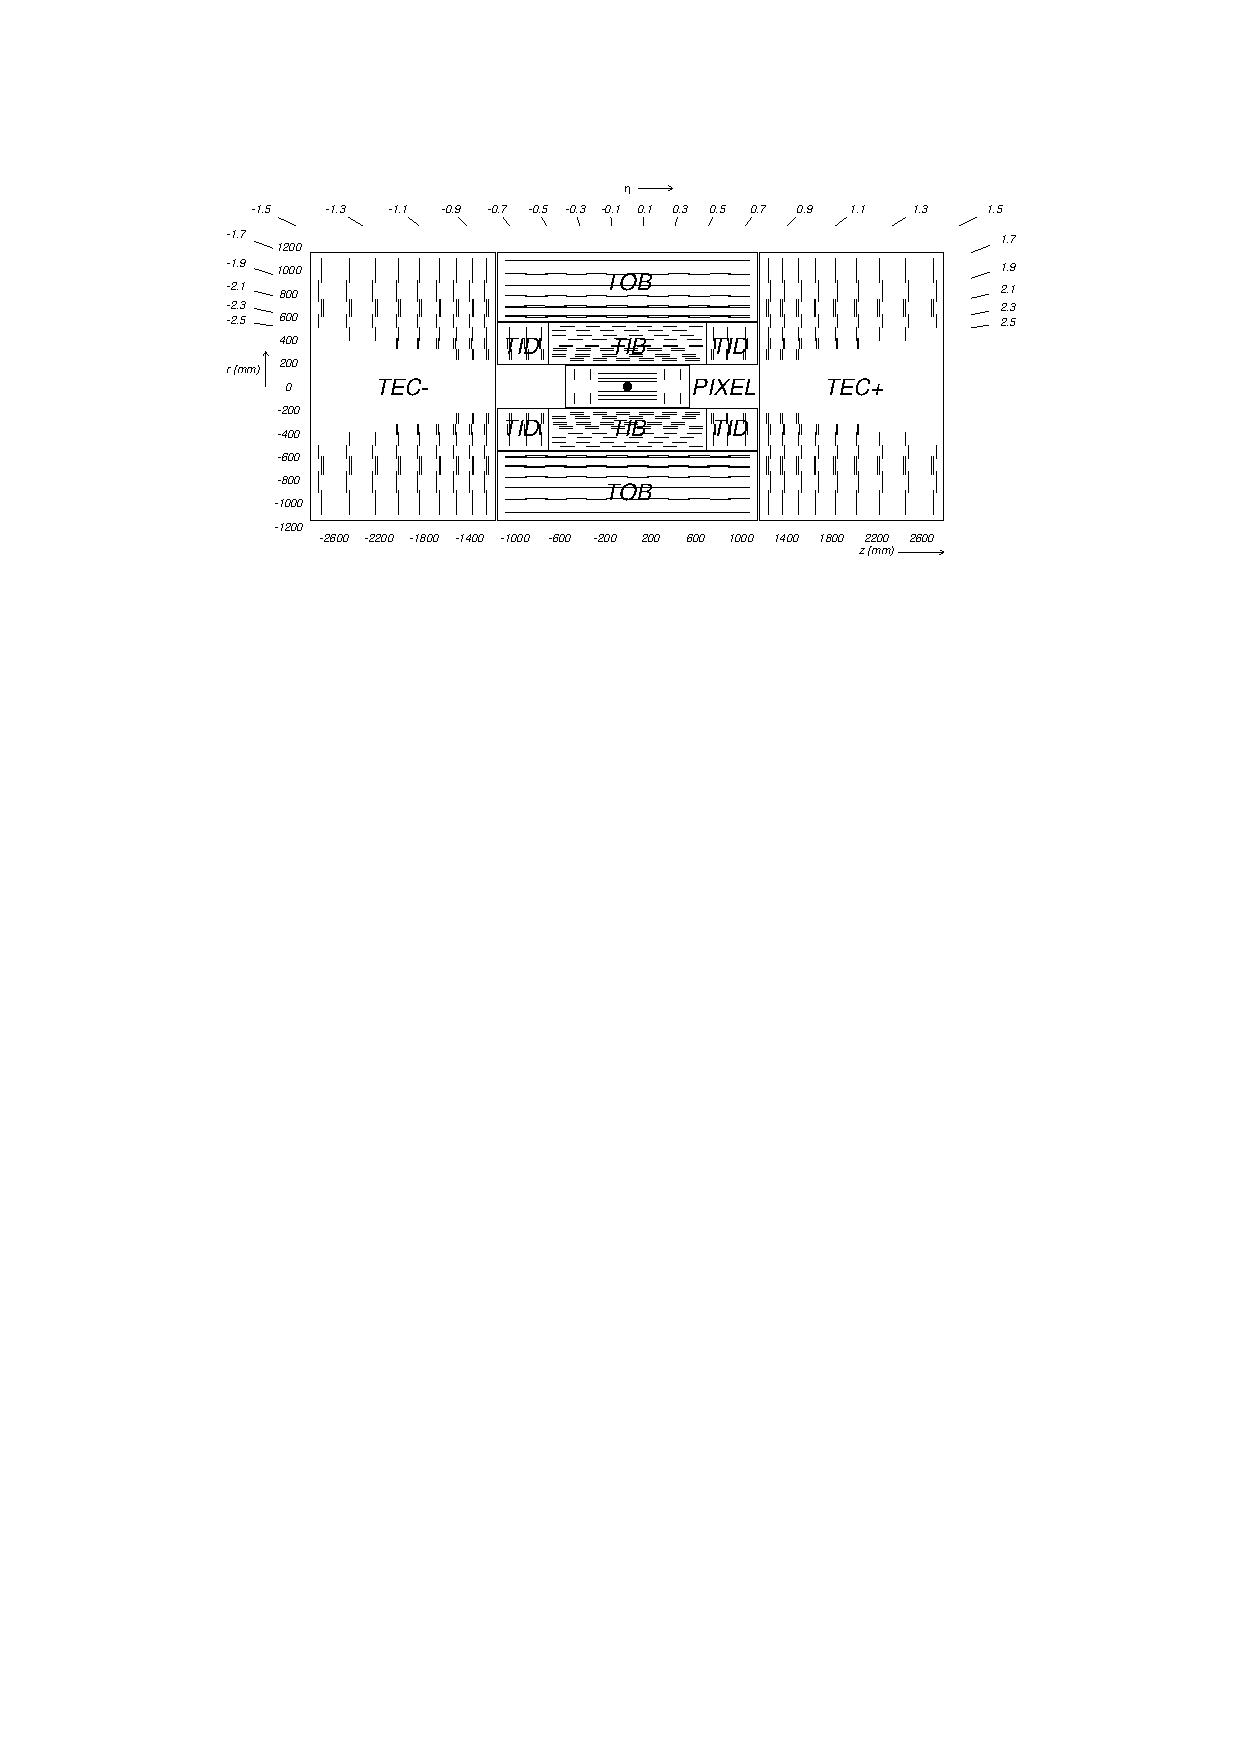
\includegraphics[width=0.9\textwidth]{figures/cms_tracker.pdf}
\caption{Layout of the CMS tracker. From \cite{Chatrchyan:2008aa}.}
\label{fig:cms_tracker}
\end{figure}

\subsection{Electromagnetic calorimeter}
The electromagnetic calorimeter of CMS (ECAL) is a hermetic homogeneous calorimeter made of
61,200 lead tungstate ($\textrm{PbWO}_{\textrm{4}}$) crystals mounted in the central barrel part,
and 7,324 crystals in each of the two endcaps. 
A preshower detector is placed in front of the endcap crystals.
Avalanche photodiodes (APDs) are used as photodetectors in the barrel and vacuum phototriodes
(VPTs) in the endcaps. The use of high density crystals has allowed the design of a calorimeter
which is fast, has fine granularity and is radiation resistant, all important characteristics in the LHC
environment. 
One of the driving criteria in the design was the capability to detect the decay to two
photons of the postulated Higgs boson.
This capability is enhanced by the good energy resolution
provided by a homogeneous crystal calorimeter.

\begin{figure}
\centering
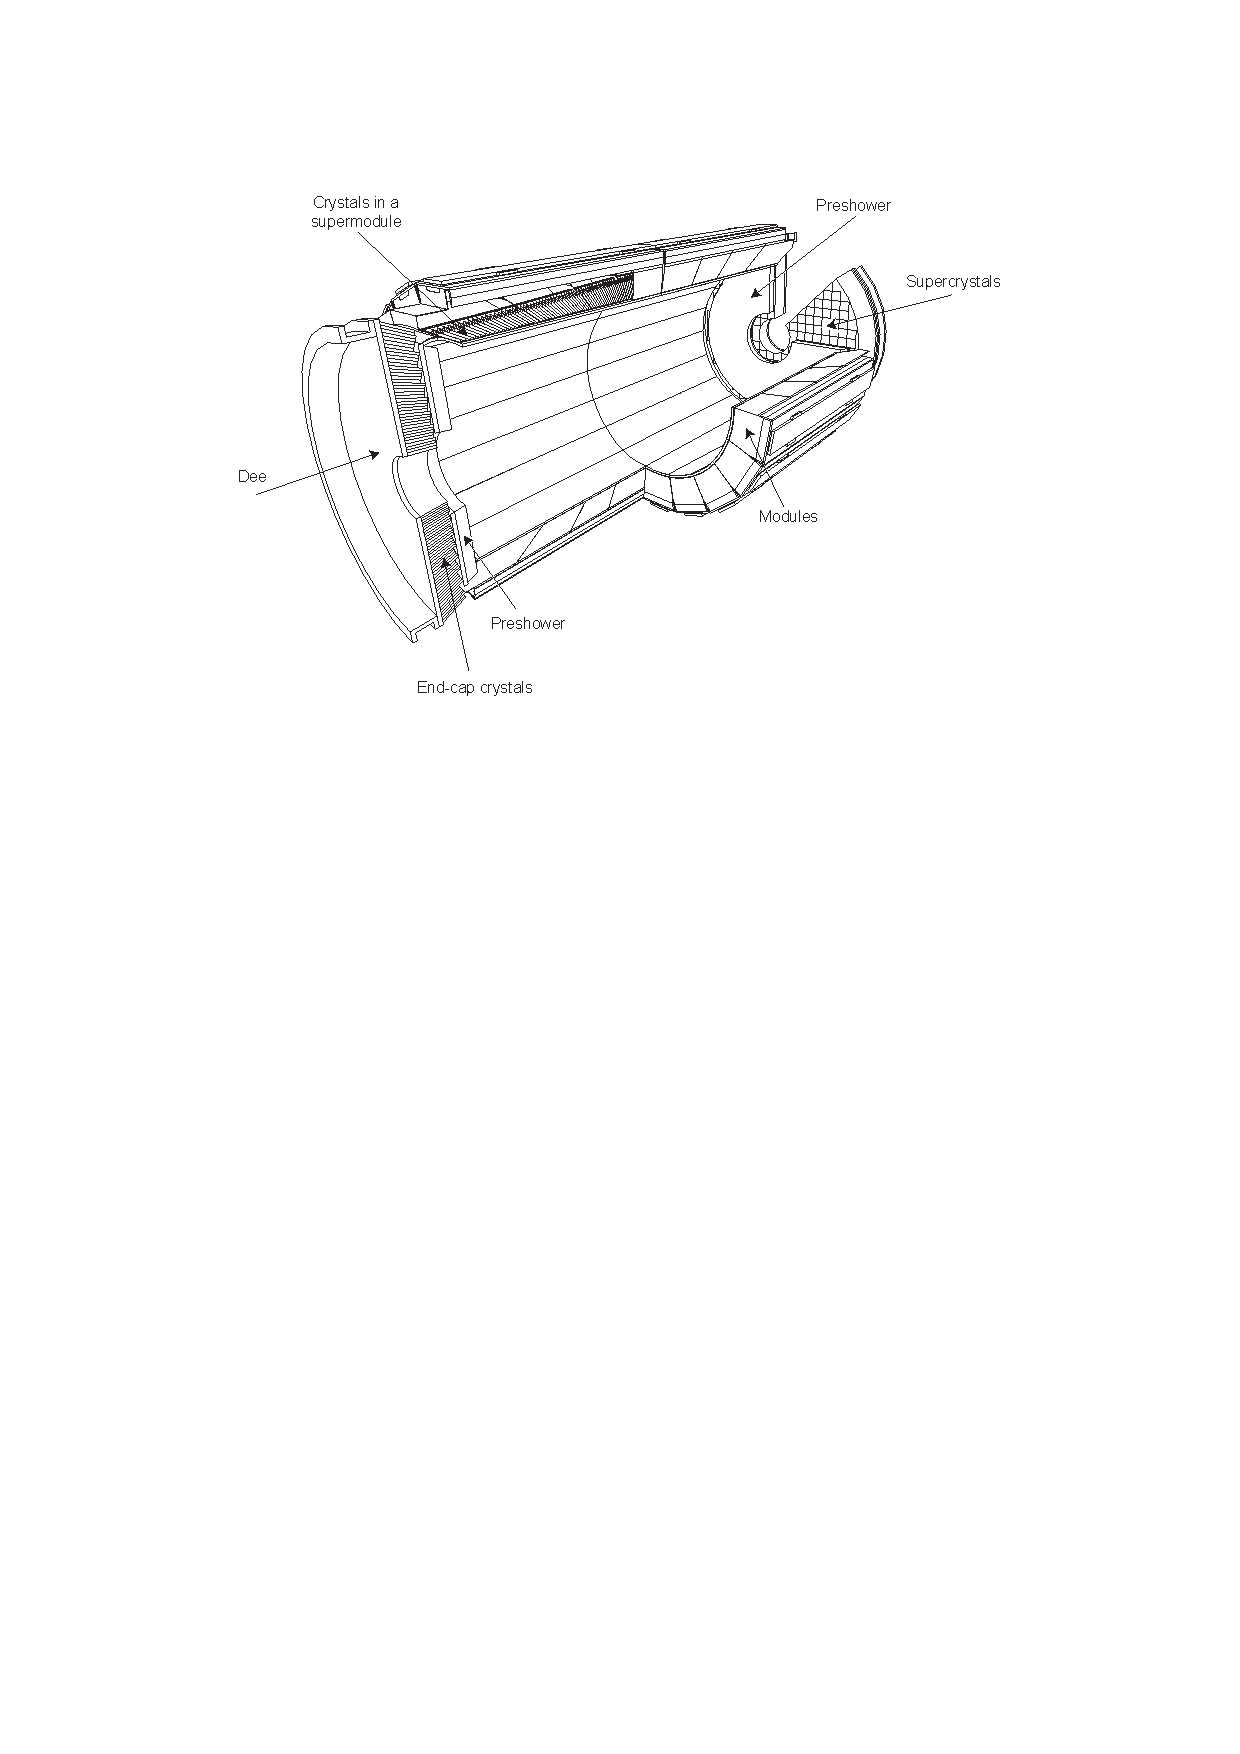
\includegraphics[width=0.9\textwidth]{figures/ecal_layout.pdf}
\caption{Layout of the CMS electromagnetic calorimeter showing the arrangement of crystal
modules, supermodules and endcaps, with the preshower in front. From \cite{Chatrchyan:2008aa}.}
\label{fig:ecal_layout}
\end{figure}

The number of scintillation photons and the electronic amplification thereof both are decreasing with temperature. 
So the ECAL must be kept at a stable temperature of $18\pm0.05$\textdegree~ C.
Water cooling and aluminum tubing are used to meet this need.

\subsubsection{ECAL barrel}
The ECAL barrel (EB) covers the pseudorapidity range $|\eta|<1.479$.
The granularity is 360 in $\phi$ and 170 in $\eta$, giving 61,200 crystals in all.
The crystals have a tapered shape.
They are mounted in a quasi-projective geometry to avoid cracks aligned with particle trajectories.
In other words, their central axes are not exactly parallel to a path from the interaction point, 
in either the $\phi$ or $\eta$ projections.
The crystal cross-section corresponds to approximately $0.0174 \times 0.0174$ in $\eta\times\phi$
or $22 \times 22$ mm\textsuperscript{2} at the front face of the crystal--and $26 \times 26$ mm\textsuperscript{2}
at the rear face.
The crystals' radial length is 230 mm, corresponding to 25.8 radiation lengths.

\begin{figure}
\centering
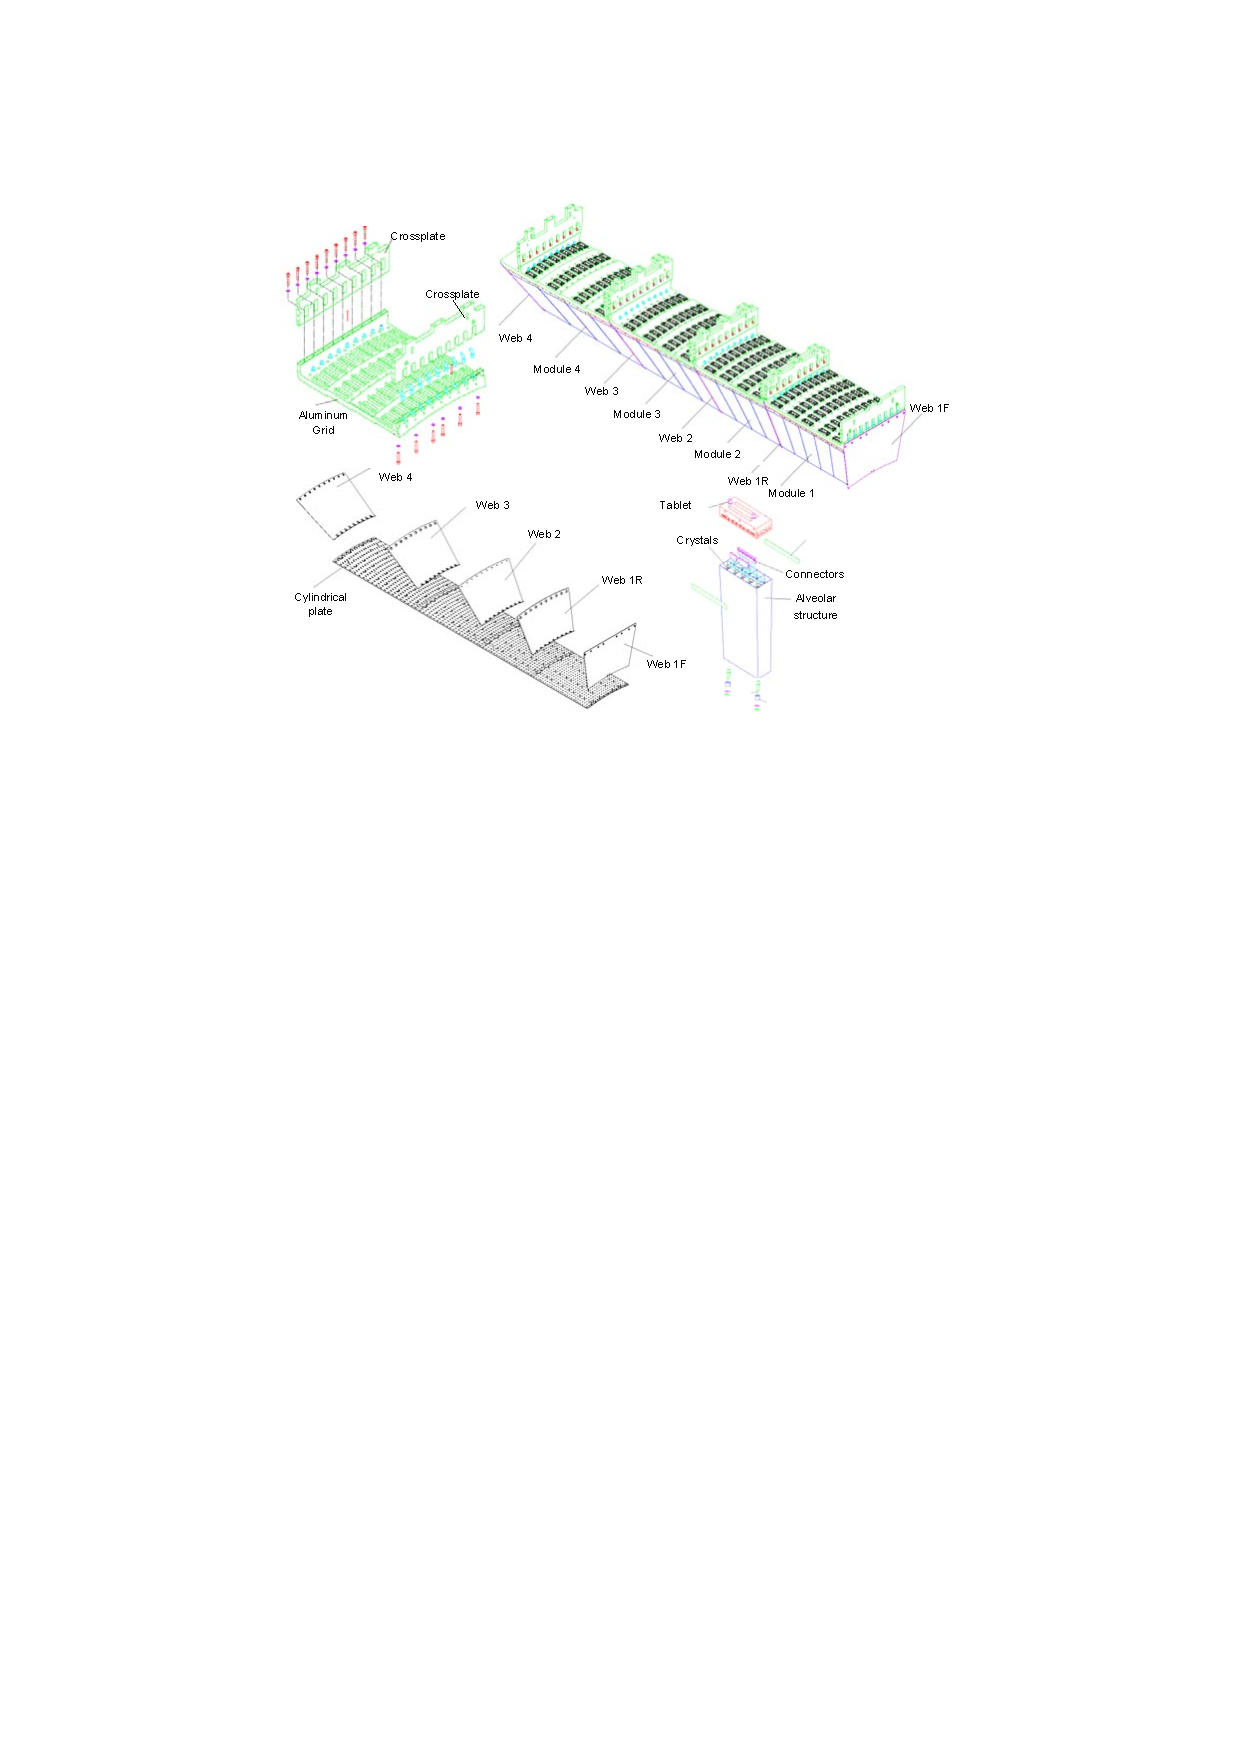
\includegraphics[width=0.9\textwidth]{figures/ecal_barrel.pdf}
\caption{Layout of the ECAL barrel. From \cite{Chatrchyan:2008aa}.}
\label{fig:ecal_barrel}
\end{figure}

In the barrel, the scintillation photons are collected by Hamamatsu type S8148 reverse structure avalanche photodiodes.
Their active area is $5\times5$ mm\textsuperscript{2}. Two are mounted on each crystal.

\subsubsection{ECAL endcaps}
The ECAL endcaps (EE) cover the rapidity range $1.479 < \eta < 2.5$.
The distance from the interaction point and the endcaps is 315.4 cm with the 4 T magnetic field on.
Most of each endcap consists of identically shaped crystals grouped in mechanical units of $5\times5$ crystals, called supercrystals.
As with the EB crystals, the central axes of the EE supercrystals are not exactly parallel to a path from the interaction point. 
The front face of these crystals has an area of $28.62\times28.62$ mm\textsuperscript{2}.
The rear face has an area of $30\times30$ mm\textsuperscript{2}.
The crystals' length is 220 mm or 24.7 radiation lengths.

In the endcaps, the scintillation photons are collected by type PMT188 vacuum phototriodes
from National Research Institute Electron in St. Petersburg.
Their active area is 280 mm\textsuperscript{2}. One is mounted on each crystal.

It is relevant to make a note here that the physical cracks between the EB and EEs exist at $1.4442 < |\eta| < 1.566$. 
This has a negative effect on the electron identification efficiency, to be described in great detail later.
This motivates the non-intuitive kinematic binnings in $\eta$ which are used later
in Chapter~\ref{chap:efficiency} and Appendix~\ref{app:efficiency}.

\subsection{Hadron calorimeters}
The hadron calorimeters (HCALs) exist to measure the energy of hadrons and hadronic jets.
Most hadrons pass through the ECAL due to its limited stopping power and then deposit the rest of their energy in the HCAL.
Muons, and the few energetic hadrons which punch through the HCAL, traverse past it and reach the muon system.
From the visible particle energies recorded in the ECAL, HCAL, and muon systems, 
it is possible to construct the quantity of missing transverse energy in order to
infer the production of neutrinos or exotic particles.
Figure~\ref{fig:hcalslice} shows the longitudinal view of the CMS detector. The dashed lines are at fixed $\eta$ values. 
The hadron calorimeter barrel and endcaps sit behind the tracker and the electromagnetic
calorimeter as seen from the interaction point. The hadron calorimeter barrel is radially restricted
between the outer extent of the electromagnetic calorimeter (R = 1.77 m) and the inner extent of
the magnet coil (R = 2.95 m). This constrains the total amount of material which can be put in
to absorb the hadronic shower. Therefore, an outer hadron calorimeter or tail catcher is placed
outside the solenoid complementing the barrel calorimeter. Beyond $|\eta| = 3$, the forward hadron
calorimeters placed at 11.2 m from the interaction point extend the pseudorapidity coverage down
to $|\eta| = 5.2$ using a Cherenkov-based, radiation-hard technology.
The HCAL subsystems are described briefly below, with more detailed information on the geometry and 
readout being available in~\cite{CMSTDR}.

\begin{figure}
\centering
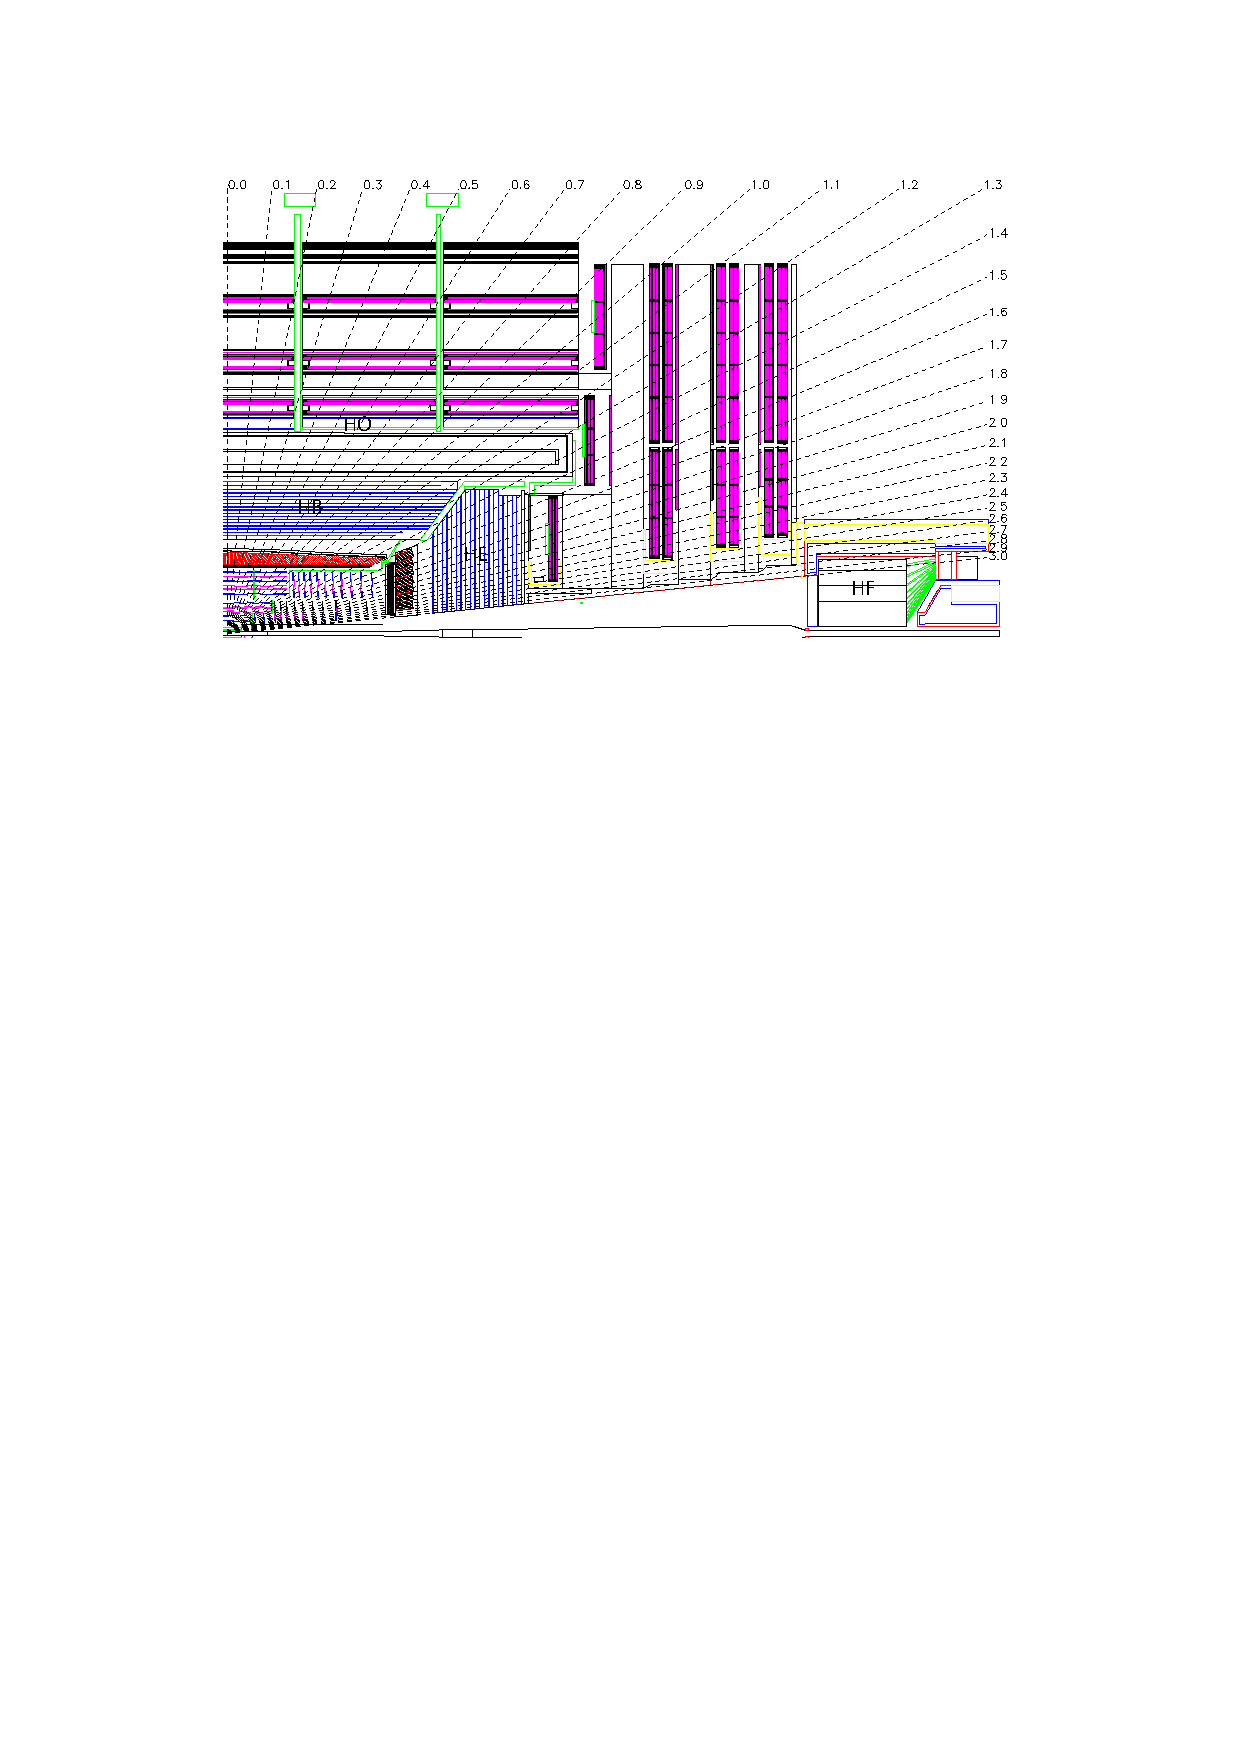
\includegraphics[width=0.98\textwidth]{figures/hcalslice.pdf}
\caption{Longitudinal slice of the CMS detector showing the locations of the hadron barrel
(HB), endcap (HE), outer (HO) and forward (HF) calorimeters.}
\label{fig:hcalslice}
\end{figure}

\subsubsection{HCAL barrel}
The HCAL barrel (HB) is a sampling calorimeter and covers the pseudorapidity range $|\eta| < 1.3$.
It consists of 36 identical azimuthal wedges which form two half-barrels. 
The wedges are constructed out of flat brass absorber plates which are parallel
to the beam axis.  Each wedge is segmented into four azimuthal angle ($\phi$) sectors. 
The innermost and outermost plates are made of stainless steel for structural strength.

The absorber consists of a front steel plate 40 mm thick,
followed by eight 50.5 mm thick brass plates, six 56.5 mm thick brass plates,
and a 75 mm thick steel back plate.
The last layer is thicker to correct for late developing showers which could leak out the back.
The total absorber thickness at 90\textdegree~is 5.82 interaction lengths ($\lambda_I$).
The HB effective thickness increases with polar angle ($\theta$) as $1/\textrm{sin}\:\theta$,
resulting in 10.6 $\lambda_I$ at $|\eta| = 1.3$. 

The HB baseline active material is 3.7 mm thick Kuraray SCSN81 plastic scintillator, 
chosen for its long-term stability and moderate radiation hardness. 
The first layer of scintillator is located in front of the steel support plate, 
and is made of 9 mm thick Bicron BC408. 
Its purpose is to sample hadronic showers developing in the inert material between
the ECAL barrel and the HCAL barrel.
The plastic scintillator is divided into 16 $\eta$ sectors, resulting in a segmentation of $(\Delta\eta, \Delta\phi) = (0.087, 0.087)$. 

\subsubsection{HCAL endcaps}

The hadron calorimeter endcaps (HE) cover the rapidity range $1.3 < |\eta| < 3$. 
It is designed for high radiation tolerance, in order to survive 10 MRad after 10 years of operation.
The total length of the endcap calorimeter, after the ECAL and HCAL endcaps, is about 10 interaction lengths. 

The absorber is made of C26000 cartridge brass. The material was chosen because it is non-magnetic, has a short interaction length and was available at a relatively low cost.
The absorber is assembled in a staggered geometry which minimizes the cracks between HB and HE and contains no projective dead material. 

The scintillators are of trapezoidal shape and there are 18 layers of them in total. 
The first layer are made of 9 mm thick Bicron BC408. All the rest are made of 3.7 mm thick SCSN81.
The scintillation light is read out via wavelength shifting fibers. 
The granularity of the calorimeters is $(\Delta\eta, \Delta\phi) = (0.087, 0.087)$ for $|\eta| < 1.6$ and $(\Delta\eta, \Delta\phi) = (0.170, 0.170)$ for $|\eta| \geq 1.6$.

\subsubsection{HCAL outer}
The combined stopping power of the ECAL and HCAL barrels does not provide adequate stopping
power in the central region $|\eta| < 1.3$. This is problematic for the missing energy resolution.
To further measure and contain these showers, the hadron calorimeter is extended outside the solenoid with a tail catcher called the HO. Only 40 mm of space in the radial direction is available, 
24 mm of which is used for aluminum honeycomb support structures.

The scintillator plates of the HO are made of 10 mm thick Bicron BC408. There are 5 rings in $\eta$, each of those rings having 12 identical $\phi$ sectors, and each of those sectors having 6 azimuthal slices.
The sizes and positions of the tiles in HO are supposed to roughly map the layers of HB
to make towers of granularity $(\Delta\eta, \Delta\phi) = (0.087, 0.087)$.

The magnetic solenoid coil is used as an additional absorber equal to $1.4/\textrm{sin}\:\theta$ interaction lengths.
Outside the vacuum tank, the magnetic field is returned through an iron yoke roughly 20 mm thick, with 5 rings corresponding to the scintillator plates.
The central ring has scintillators both inside and outside of the iron yoke ring.
The others have scintillators only outside their yoke rings.
All told, the total depth of the calorimeter system is extended to a minimum of
$11.8\:\lambda_I$ except at the barrel-endcap boundary region at around $|\eta|=1.4$.

\subsubsection{HCAL forward}
The forward calorimeter, or HF, exists in an extremely hostile environment. 
At $|\eta|=5$ we expect to have delivered 10 MGy after 10 years of operation.
The active material is fused-silica core, polymer hard-cladded quartz fibers, which have sufficient radiation hardness.
These fibers measure 600 $\pm$ \SI{10}{\micro\meter} in diameter for the fused-silica core,
$ {630}^{+5}_{-10}$ \SI{}{\micro\meter} with the polymer hard-cladding, 
and 800 $\pm$ \SI{30}{\micro\meter} with the protective acrylate buffer.

The geometry consists of a steel absorber structure composed of 5 mm thick grooved
plates. Fibers are inserted in these grooves.
The detector is functionally subdivided into two longitudinal segments. 
Half of the fibers run over the full depth of the absorber (165 cm $\approx 10\:\lambda_I$)
while the other half starts at a depth of 22 cm from the front of the detector.
These two sets of fibers are read out separately. 
This arrangement makes it possible to distinguish showers generated by electrons and photons,
which deposit the majority of their energy in the first 22 cm,
from those generated by hadrons, which produce nearly equal signals in both calorimeter segments on average. 
The absorber has grooves which make a square grid separated by 5.0 $\pm$ 0.1 mm center-to-center, with long and short fibers alternating in the grooves. 

This calorimeter is mostly sensitive to the electromagnetic component of hadronic showers.
Only light that hits the core-cladding interface at an angle larger than the critical angle (71\textdegree) contributes to the calorimeter signal in the form of Cherenkov light. 
After the quoted 10 MGy dose has accumulated over the HF lifetime, the optical transmission of the fibers is reduced just by a factor of 2.

\subsection{Muon system}
\label{ss:muonsystem}
The CMS muon system is capable of reconstructing the momentum and charge of muons over the entire
kinematic range of the LHC. 
Due to the shape of the CMS solenoid magnet, the muon system has a barrel section and 2 endcap sections.
Three types of gaseous particle detectors are used.
Since the total area of the muon detection planes is around 25,000 $\textrm{m}^2$, the 
detectors were chosen to be inexpensive but reliable.

In the barrel region, rectangular drift tubes (DT) are used, 
since there is little neutron-induced muon background, the magnetic field is uniform,
and the real muon rate is relatively low.
In the endcap regions, there is a high muon rate, high muon background, and a
very nonuniform magnetic field, so cathode strip chambers (CSC) are used there.
The third subsystem is the resistive plate chambers (RPC). Their spatial resolution is relatively poor.
But their fast response and good time resolution are useful for the trigger.
They also help resolve ambiguity in the standalone muon reconstruction,
which only uses information from the muon system.

The DTs and CSCs are each capable of triggering on muon $p_T$ independently of the other detector subsystems.
The $p_T$ resolution of this triggering muon object is 15\% in the barrel and 25\% in the endcap.
For muon $p_T$ up to $200 \GeV$, the DTs and CSCs together can give a standalone momentum resolution of 9\%.
Approaching muon momenta of $1 \TeV$, the standalone momentum resolution is 5\%.
The muon resolution is improved when combined with the tracker information in the Particle Flow algorithm.

Lastly, an alignment system measures the relative positions of the muon detectors amidst the inner tracker to optimize the momentum resolution of muons.

\begin{figure}[hbtp]
\centering
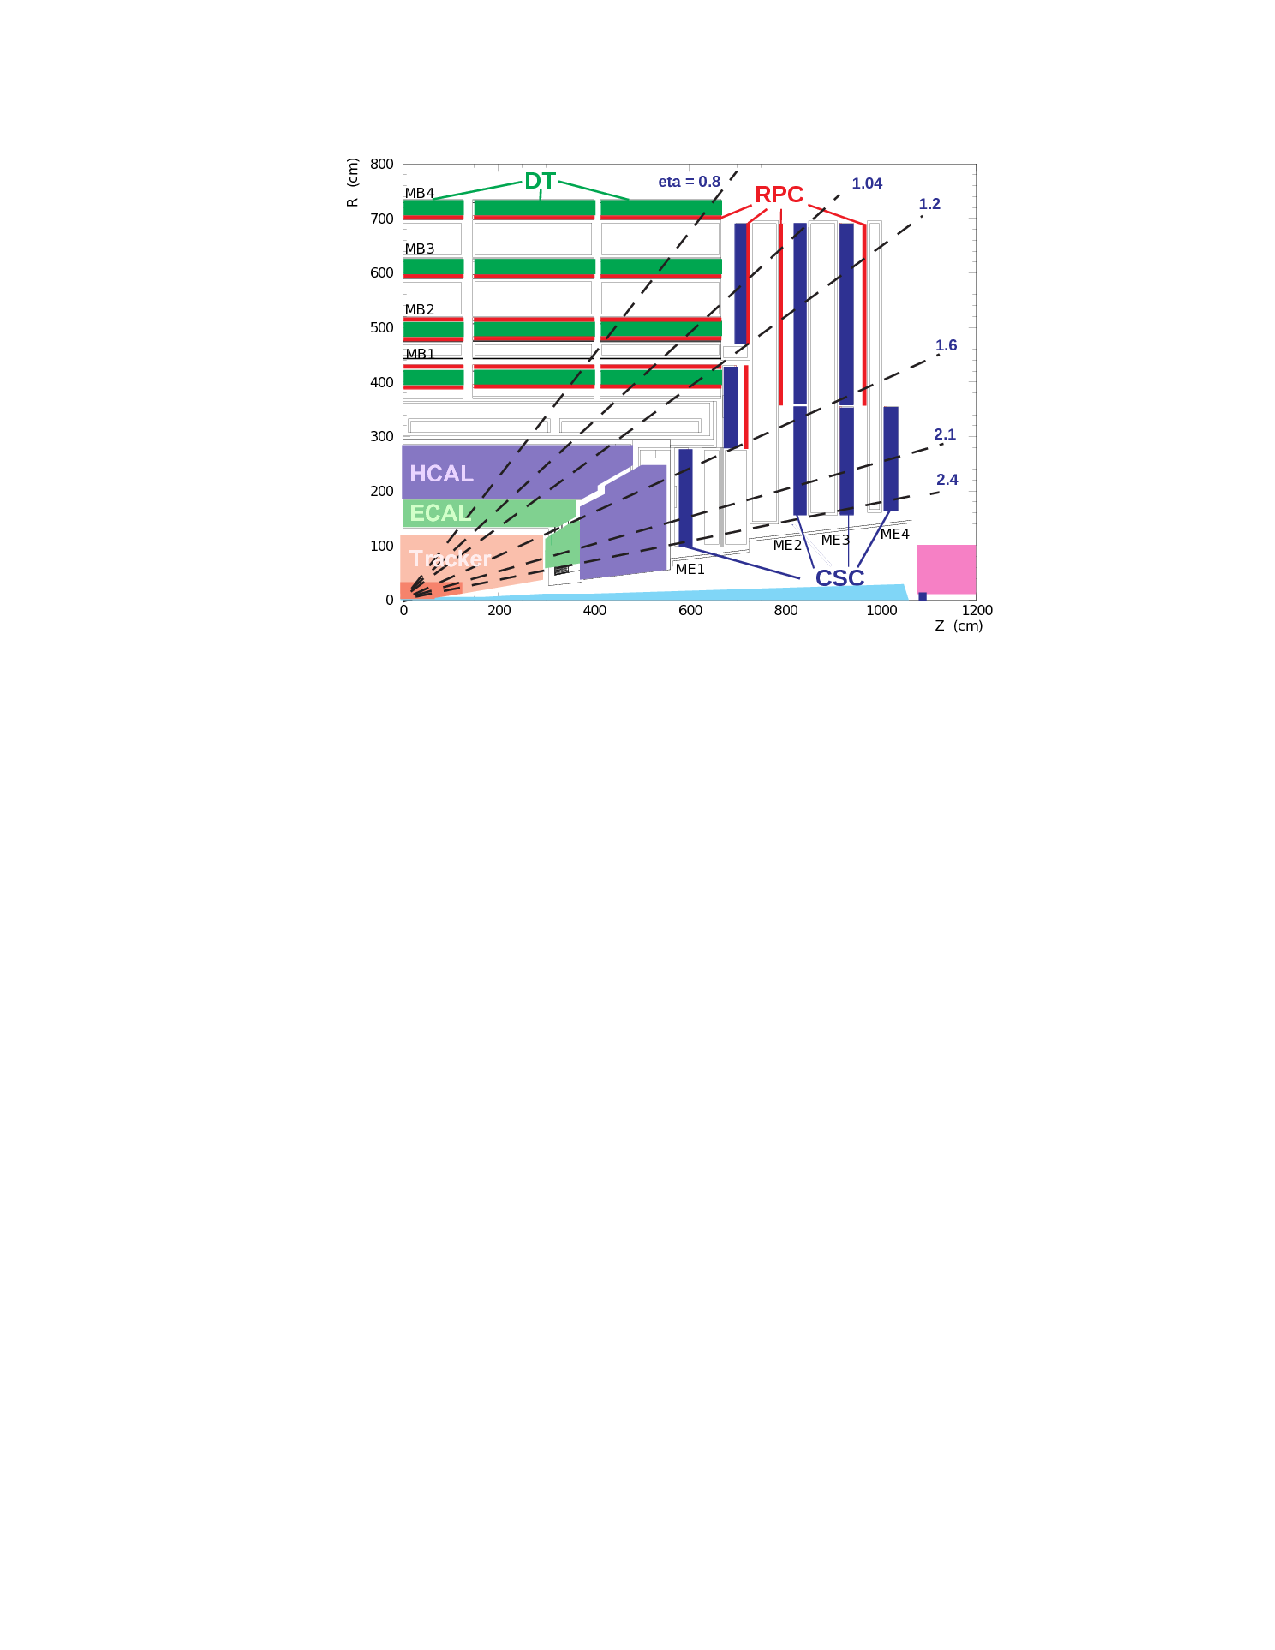
\includegraphics[width=0.8\textwidth]{figures/cms_muon_systems.pdf}
\caption{
Quarter-view of the CMS detector showing the muon system components. 
From \cite{Chatrchyan:2008aa}.
}
\label{fig:muonsystem}
\end{figure}

\subsubsection{Drift tubes}
The DTs cover the pseudorapidity region $|\eta|<1.2$.
There are 4 stations forming concentric cylinders around the beam line.
The 3 inner cylinders have 60 drift chambers each and the outer cylinder has 70.
There are about 172,000 sensitive wires of about 2.4m in length.
The maximum drift path length is 21 mm. In a gaseous admixture of 85\% Ar and 15\% $\mathrm{CO}_2$ the maximum drift time is 380 ns.
This produces a negligible occupancy and permits the use of single-hit electronics.
Meanwhile, the cell size is sufficiently large to keep the number of electronic channels low and affordable.

Each DT chamber is made of 2 or 3 superlayers (SL).
Each SL is made of layers of rectangular drift cells staggered by half a cell.
The wires in the 2 outer SLs are parallel to the beam line and provide a track measurement
in the magnetic bending plane. 
The wires in the inner SL are orthogonal to the beam line and measure the $z$ position.
This innermost SL is not present in the fourth DT station
Thus, a muon first encounters a $\phi$-measuring SL, passes through a honeycomb spacer plate,
then crosses the $z$-measuring SL and the second $\phi$-measuring SL.
Due to discontinuities in the design,
a muon could end up crossing only two stations instead of the maximum four.

One superlayer has time resolution on the order of nanoseconds.
The time measurement is delayed by the drift-time, determined by the design parameters of the drift tubes.
Using the SL information, pattern recognition circuits deliver the position and angle 
of the track segment's center of gravity with precision of 1.5 mm and 20 mrad, respectively.

\begin{figure}[hbtp]
\centering
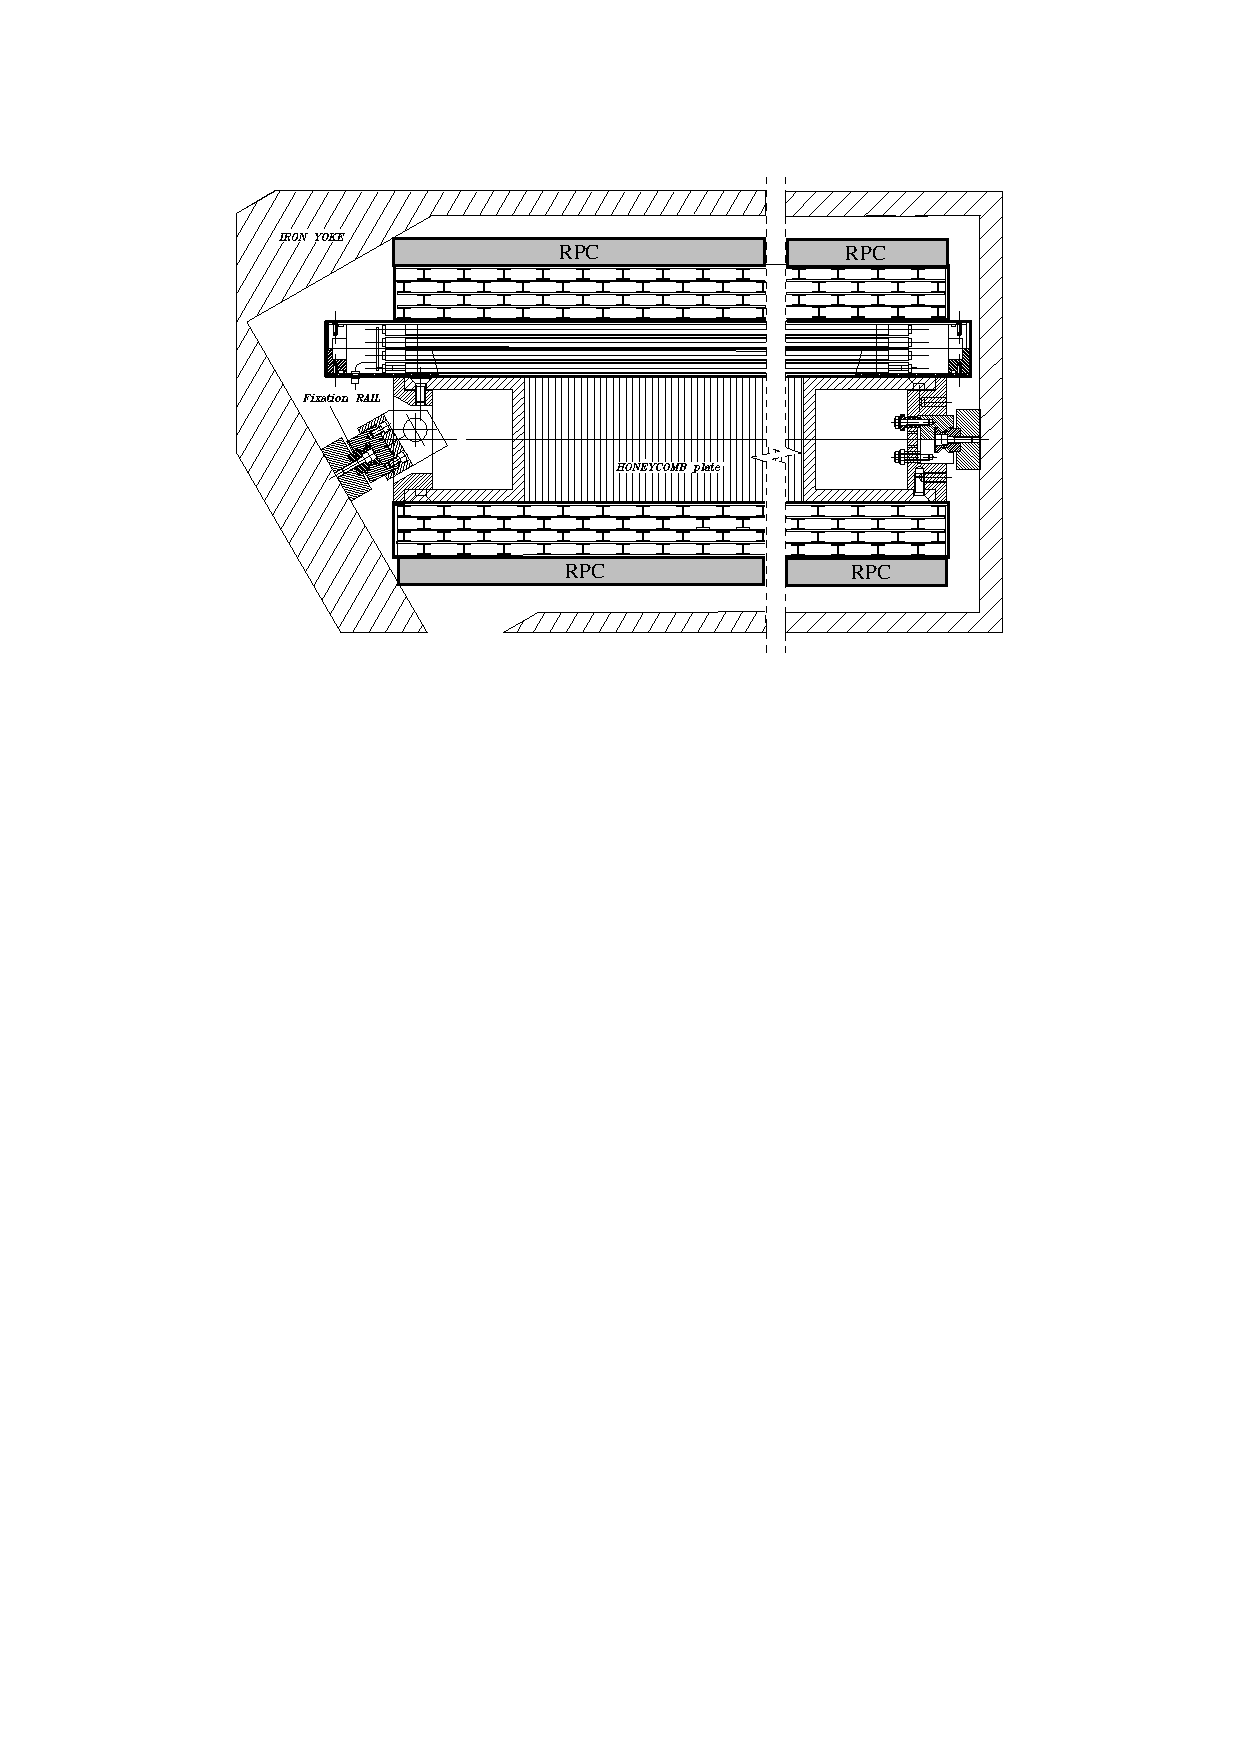
\includegraphics[width=0.80\textwidth]{figures/cms_muonsystem_honeycomb.pdf}
\caption{Chambers of the CMS DT system including the honeycomb support. From \cite{Chatrchyan:2008aa}.}
\label{fig:dt_chambers}
\end{figure}

\begin{figure}[hbtp]
\centering
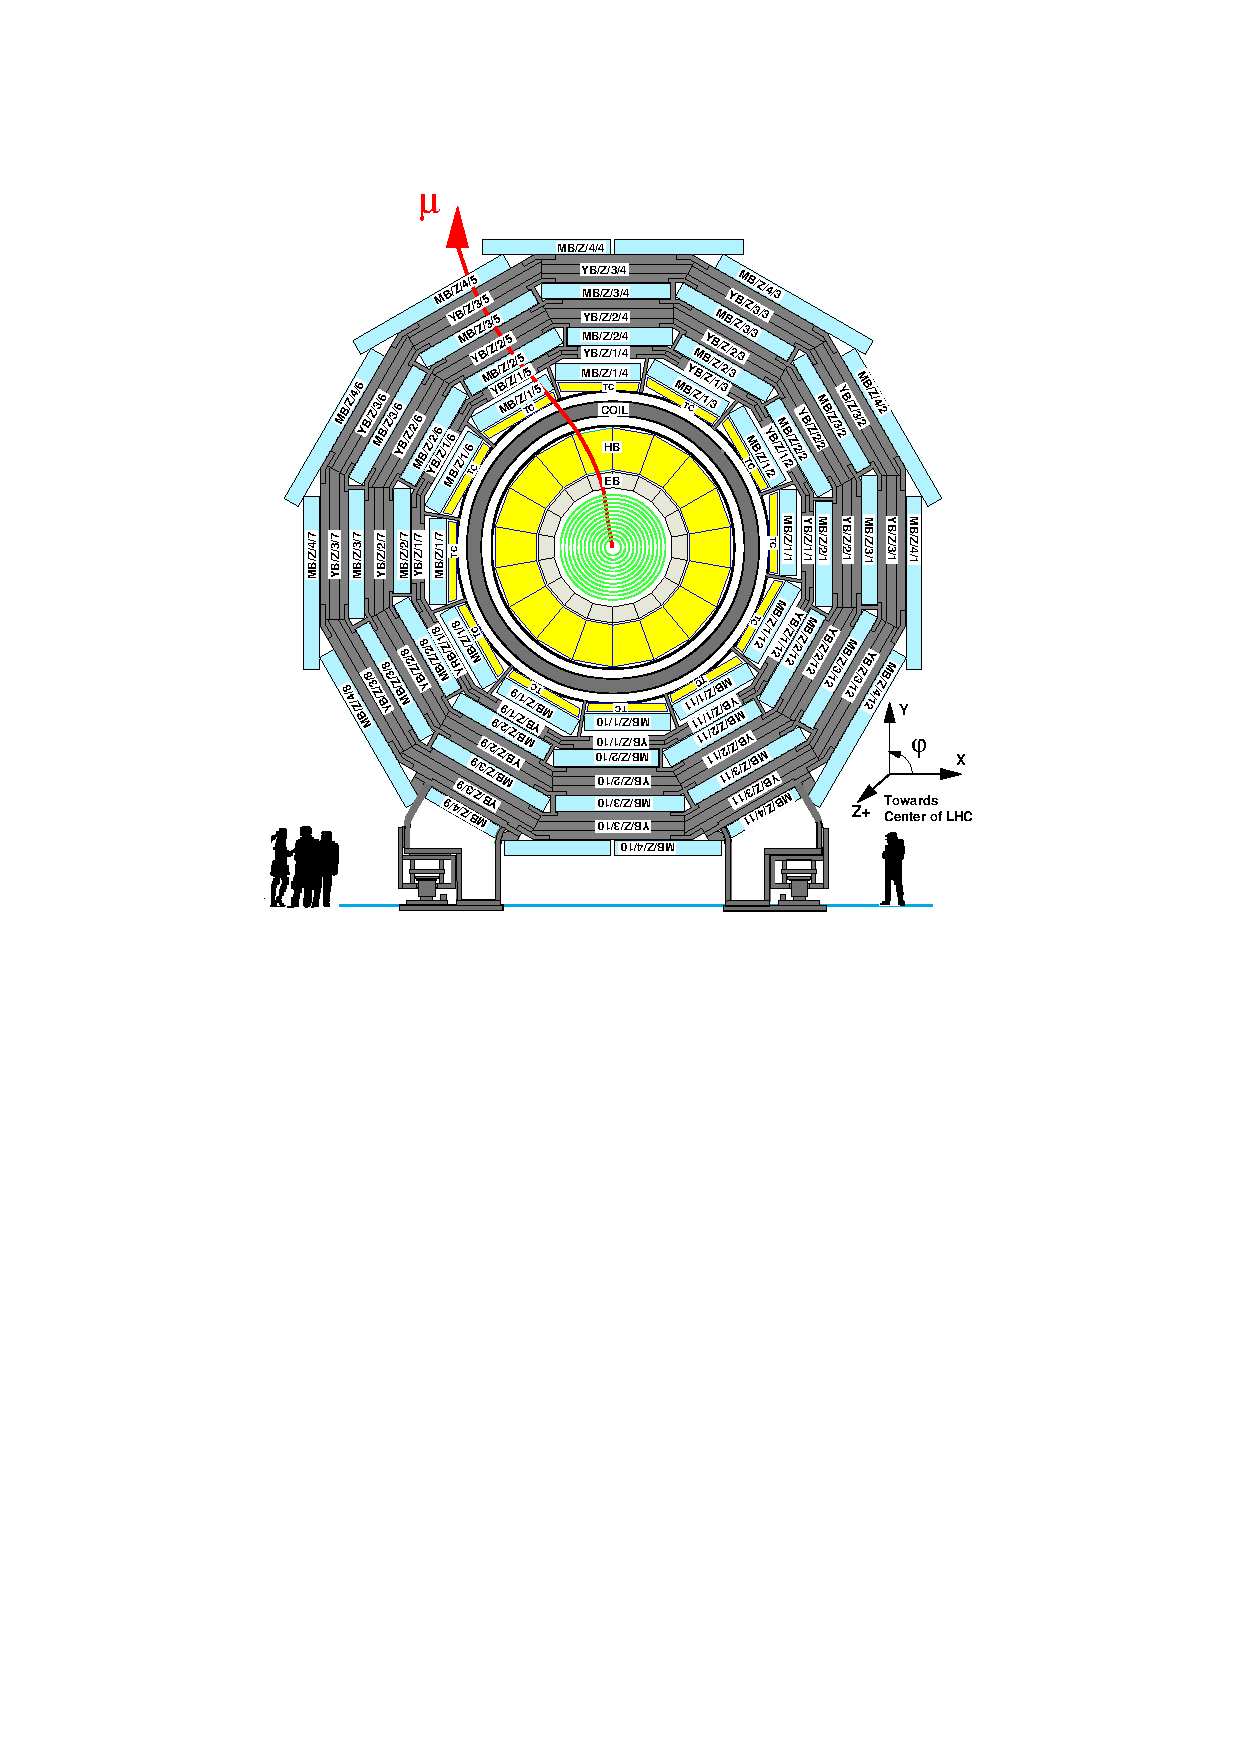
\includegraphics[width=0.8\textwidth]{figures/cms_drifttubes_slice.pdf}
\caption{ Layout of the CMS barrel muon DT chambers in one of the 5 wheels. From \cite{Chatrchyan:2008aa}.}
\label{fig:dt_barrel}
\end{figure}

\subsubsection{Cathode strip chambers}
The CSCs cover the pseudorapidity region $0.9<|\eta|<2.4$.
There are 4 stations of CSCs in each endcap.
The chambers are perpendicular to the beamline and interspersed between the magnetic flux return plates.
The cathode strips point radially outward from the beamline and provide a precision measurement in the $r-\phi$ bending plane.

The CSCs are multiwire proportional chambers comprised of 6 anode wire planes interleaved
among 7 cathode panels. Wires run azimuthally and define a track’s radial coordinate.
Strips are milled on cathode panels and run lengthwise at constant $\Delta\phi$ width. 
The muon coordinate along the wires is obtained by interpolating between charges induced on strips.
The largest chambers, ME2/2 and ME3/2, are about 3.4 × 1.5 m\textsuperscript{2} in size.
The overall area covered by the sensitive planes of all chambers is about 5,000 m\textsuperscript{2},
the gas volume is over 50 m\textsuperscript{3}, and there are about 2 million wires.
There are about 9000 high-voltage channels in the system, 
about 220,000 cathode strip read-out channels with 12-bit signal digitization,
and about 180 000 anode wire read-out channels.

An avalanche on a wire induces charge on a cathode plane.
The charge shape can be approximately parameterized by the Gatti function~\cite{GATTI197983}.
Given the CSC geometry, most of the induced charge is shared among three or four strips.
A strip signal waveform is sampled and digitized every 50 ns.
The overal pulse duration is about 300 ns.
The charge cluster is fit to obtain the spatial coordinate, time, and cluster charge.
Using this method, the spatial resolution for a 6-plane chamber is 80 $\mathrm{\mu m}$.

\begin{figure}[hbtp]
\centering
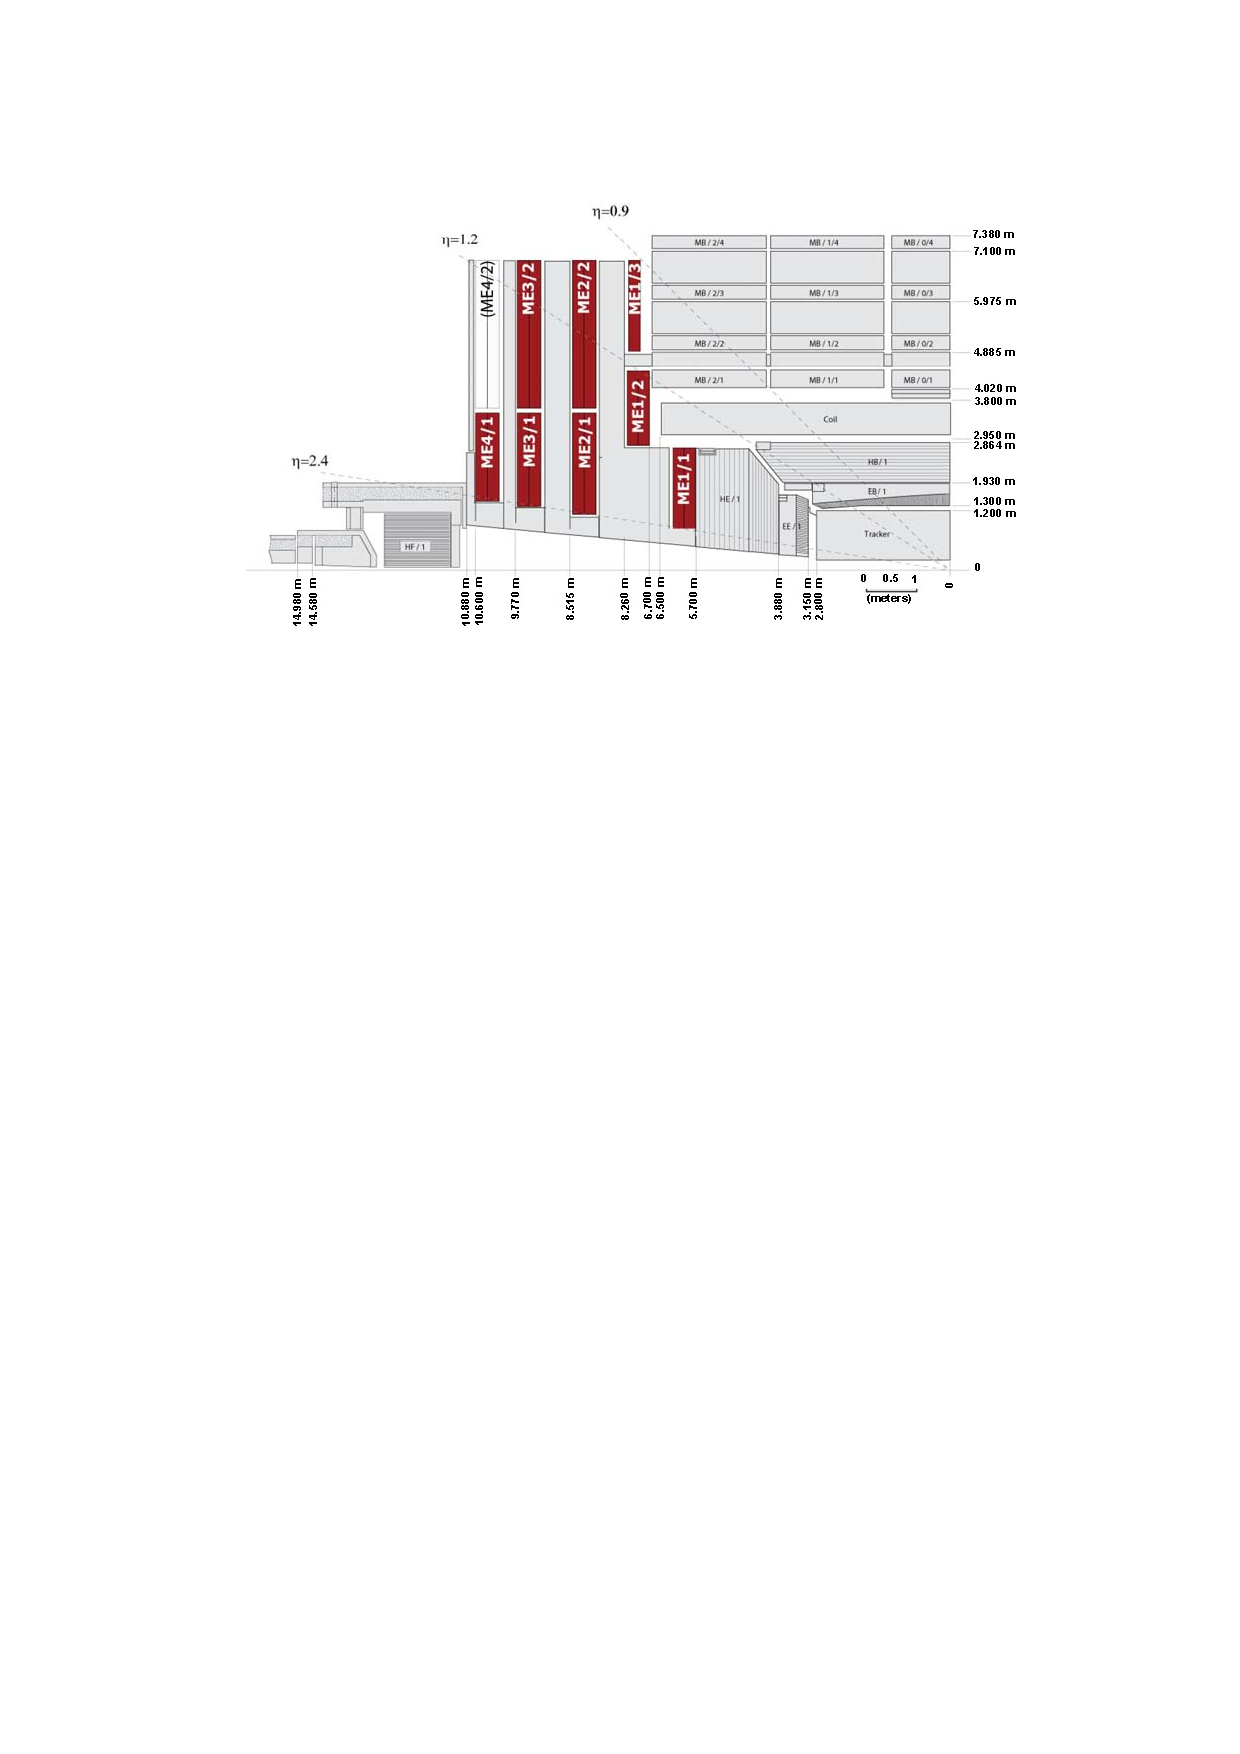
\includegraphics[width=0.8\textwidth]{figures/cms_quarter_csc_red.pdf}
\caption{
Quarter-view of the CMS detector. Cathode strip chambers of the Endcap Muon
system are highlighted.
From \cite{Chatrchyan:2008aa}.
}
\label{fig:cms_quarter_csc_red}
\end{figure}

\begin{figure}[hbtp]
\centering
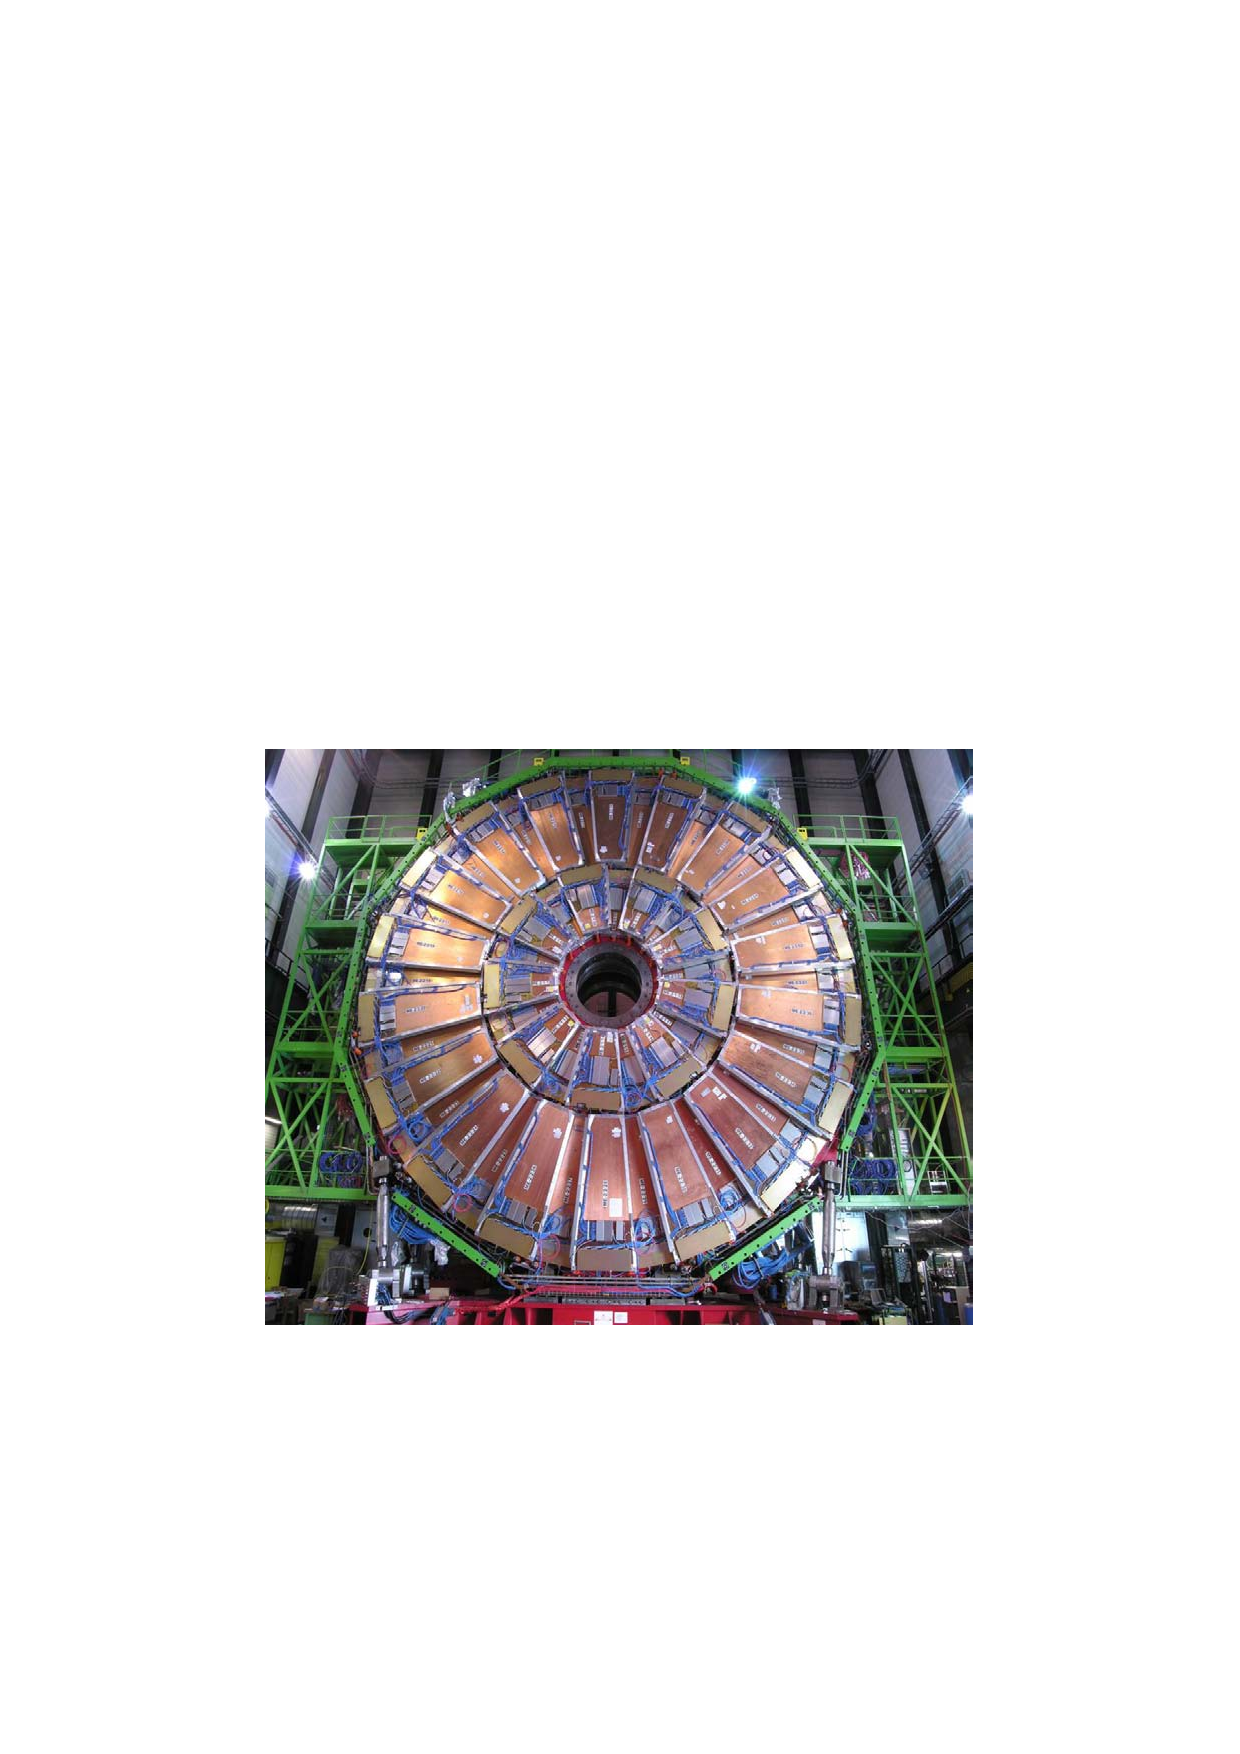
\includegraphics[width=0.8\textwidth]{figures/cms_cscs_me2.pdf}
\caption{
The ME2 station of CSCs. The outer ring consists of 36 ME2/2 chambers, each
spanning 10\degree in $\phi$, and the inner ring of eighteen 20\degree ME2/1 chambers.
The chambers overlap to provide contiguous coverage in $\phi$.
From \cite{Chatrchyan:2008aa}.
}
\label{fig:cms_cscs_me2}
\end{figure}

\subsubsection{Resistive plate chambers}

The RPCs are gaseous parallel-plate detectors with adequate spatial resolution and scintillator-level time resolution.
They are much faster than the 25 ns proton bunch crossing period at the LHC.
Using the RPC information, there is no ambiguity in the association of muon tracks and bunch crossings.

The CMS RPC basic double-gap module consists of two gaps operated in avalanche mode with common
pickup readout strips between them.
The total induced signal is the sum of the two single-gap signals.
Thus, the single-gaps can operate at a lower voltage gap,
with better effective efficiency than a single gap.

In the barrel iron return yoke, the RPC chambers form 6 coaxial sensitive cylinders
that are approximated with concentric dodecagon arrays arranged into 4 stations. See Figure~\ref{fig:cms_rpc_barrel}.

\begin{figure}[hbtp]
\centering
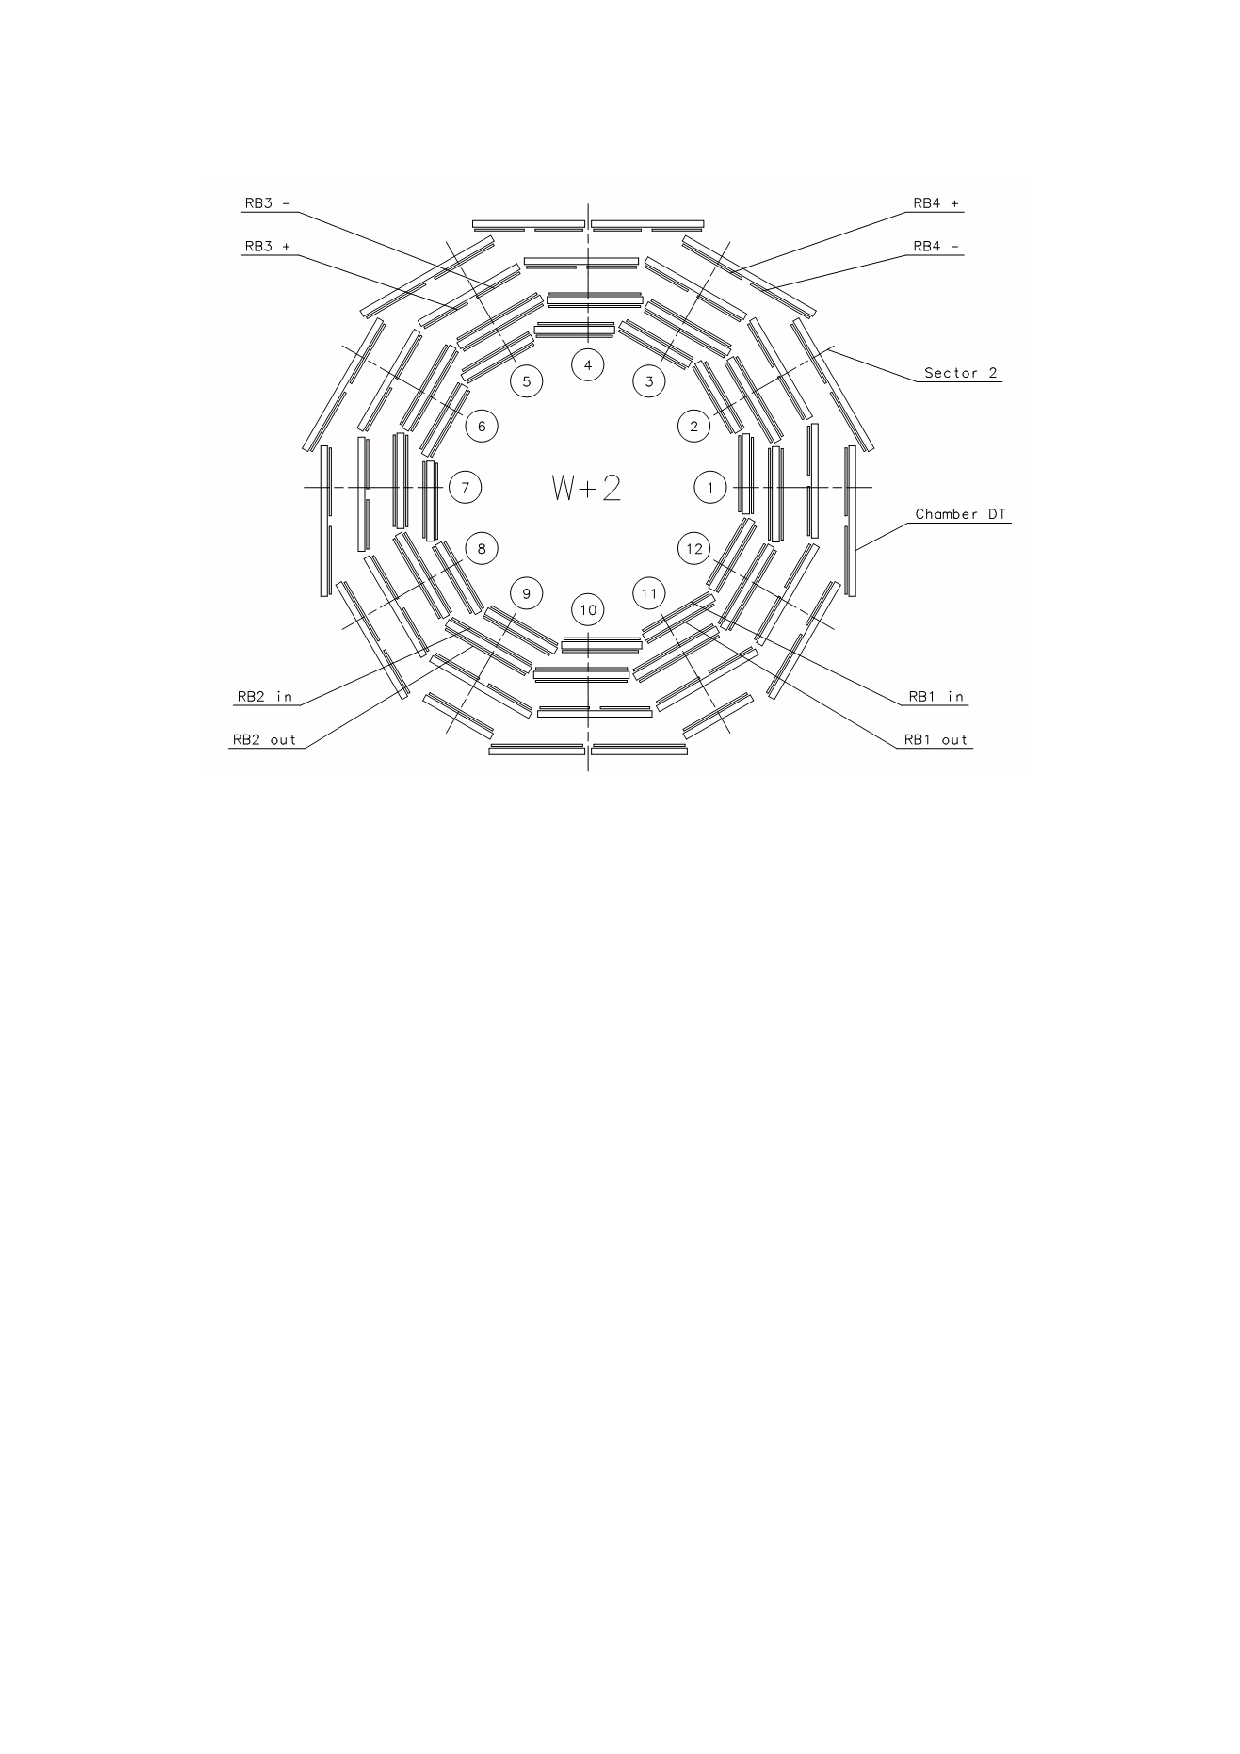
\includegraphics[width=0.8\textwidth]{figures/cms_rpc_barrel.pdf}
\caption{
Schematic layout of one of the 5 RPC barrel wheels. Each wheel is divided into 12 sectors.
From \cite{Chatrchyan:2008aa}.
}
\label{fig:cms_rpc_barrel}
\end{figure}
\clearpage

\subsection{Trigger system}
Triggering algorithms decide which data are recorded in the experiment.
They are implemented in two stages via a combination of hardware and software.

\subsubsection{Level-1 trigger}
The trigger decision process begins with the Level-1 Trigger (L1T) \cite{Khachatryan:2016bia}.  
The hardware implementation of the Level-1 Trigger is in the form of application-specific
integrated circuits (ASICs), field-programmable gate arrays (FPGAs), 
programmable logic devices (PLDs), and random access memory used for memory look-up tables (LUTs).
The FPGAs and LUTs may be reprogrammed, allowing for the algorithms to be revised.

The Level-1 Trigger is subject to a large data flow carried on optical fibers, 
copper cables, and backplanes within hardware crates. 
The data is transmitted in parallel at frequencies which are integer multiples of 40 MHz.
Data events passing the Level-1 Trigger are then transmitted to the so-called ``high-level trigger,'' described next.

\subsubsection{High-Level Trigger}
Data events accepted by the Level-1 Trigger are next processed by the High-Level Trigger (HLT).
Unlike the L1T's readout boards, the HLT is implemented on a commercial Linux computing cluster
called the File-based Filter Farm (F\textsuperscript{3}). There are three types of computing units in the F\textsuperscript{3}:
\begin{itemize}
\item The Readout Units take the information from the readout boards and assemble event fragments from a given detector partition.
\item The Builder Units take the event fragments and assemble full events. The full events are buffered here during the next step.
\item The Filter Units apply the final event selection of the HLT algorithms.
\end{itemize}
The HLT algorithms running on the FUs operate on full-granularity event data
from all subdetector systems. They accept between 1-10\% of events accepted by the L1T.
The algorithms make use of the CMS offline reconstruction framework called CMSSW.

\subsection{Offline world}
Events accepted by the HLT are merged into larger agglomerate files which are stored
locally in a Lustre parallel distributed file system.
Then, they are transferred from the ``online'' CMS experimental site to the
``offline'' CERN Tier-0 computing center at the main CERN campus in Meyrin for processing.
This transfer system is a multithreaded software,
optimized to handle rates of several gigabytes per second during data taking.
Finally, data are distributed worldwide from Tier-0 to the global CMS computing grid for physics studies.

\chapter{Data samples}
\section{The LHC and its proton injection system}


\chapter{Efficiency of lepton trigger, reconstruction, and identification}
\label{chap:efficiency}
%\autoref{chap:efficiency}
After reconstructing leptons in CMS using the information from the detector subsystems,
further offline requirements are applied for the purpose of high quality and low background lepton identification.
The choice of these requirements depends on the analysis, and several well-defined working points are optimized
and released by the relevant Physics Object Groups. The figure of merit for lepton identification is the efficiency,
and the various working points are usually described qualitatively in terms of "tightness,"
with a tighter selection corresponding to lower efficiency and higher purity.
In this note we refer to the whole slew of offline requirements applied to reconstructed leptons under the umbrella term of identification, including quantities such as relative isolation.

Previously, at lower center-of-mass energies, resonant leptonic decays of the $J/\psi$ meson were used to measure lepton identification efficiency.
In Run II at the LHC, we make use of the large cross section of the Z boson resonance and observe its leptonic decays to extract the lepton efficiencies for a wide range of lepton energies and rapidity;
while the $J/\psi$ meson is also still used for efficiency studies at lower transverse momentum.
This chapter describes how the efficiency is measured in data and simulation by studying dilepton events with invariant mass close to the Z boson resonance peak at 91.1876 $\GeV$.
The ensuing discussion presents results for the "Medium 2016" cut-based identification algorithm.

\section{Event selections for the tag-and-probe method}
\label{sec:tnpsel}
The so-called "tag-and-probe" selection consists of a high purity $\dyll$ selection with a
well-identified tag lepton and an oppositre sign probe.
The tag electron (muon) must pass the tight identification, have transverse momentum greater than 30 (25) $\GeV$, 
have $\abs{\eta}<$ 2.5 (2.4), and be matched to the leptonic trigger firing.
The probe electron must have transverse momentum greater than 10 $\GeV$ and $\abs{\eta}<$ 2.5.
For the probe muons, we consider a collection of general tracks. These tracks must have transverse momentum 
greater than 10 $\GeV$, $\abs{\eta}<$ 2.4, and a vertex whose longitudinal position is within 4 cm of that of the tag.

The selection also includes a truth-matching procedure when applied to simulated Drell-Yan samples,
so that all simulated reconstructed dileptons come from leptonic Z decays.
The reconstructed leptons must each have a small angular separation $\Delta R = \sqrt{ \Delta\phi^{2} + \Delta\eta^{2} }$ 
less than 0.3 with a final-state lepton of the same flavor at generator level. For muons, the generator-level and reconstructed
transverse momenta must also be compatible within 10\%.

\subsection{Probe multiplicity calculation}
In order to increase the signal purity of the muon selection, we perform a probe multiplicity calculation to
remove combinatorial background. The track collection as described above is considered, albeit with a 
lowered transverse momentum cut of 3 $\GeV$. Then, the number of opposite sign tag-track pairs having invariant mass above
60 $\GeV$ is counted for each tag; this gives the probe multiplicity. Any muon tags having probe multiplicity
greater than 1 are not considered in the ensuing tag and probe analysis.

\section{Control samples for the lepton efficiencies}
Two independent data samples are chosen to faithfully represent the background distributions for the
tag-and-probe fitting methods. They are defined below.
\label{sec:tnpcontrol}

\subsection{Lepton pion selection}
The mass spectrum of the combinatorial background in the Z selection can be modeled well by selecting
essentially random pairs of tag leptons and charged hadrons whose invariant mass falls within the relevant window.
We select a tag electron (muon) exactly the same as before, along with a PF charged hadron having $\pt>10~\GeV$ and $\abs{\eta}<2.5$
which must originate from the primary event vertex.

The charged hadrons selected in such a way are predominantly but not exclusively pions.
As the CMS detector does not have charged hadron particle ID capabilities beyond $\frac{dE}{dx}$,
which is ineffective for such boosted particles, we have little way of knowing if they are really pions
instead of kaons, protons, or something even more charming.
Thus, we refer to them somewhat ignorantly using $\pi^{\pm}$ as shorthand.

To obtain a data sample orthogonal to the Z selection, and to suppress contamination by Z events,
we remove events from the \ensuremath{\ell^{\pm}\pi^{\pm}} selection with the following cuts:
\begin{itemize}
\item Reject events containing a tag electron (muon) and another reconstructed electron (muon)
\item Reject \ensuremath{\pi^{\pm}} probes with separation $\Delta R$ less than 0.3 with any reconstructed electron or muon
\item Require the same charge assignment for the tag lepton and the pion probe
\end{itemize}

Furthermore, due to low event yields in this selection at higher probe energies for the electron case,
we use an $\eta$-inclusive form of this selection to build the shapes that are used in each bin of probe $\eta$ for probes with $p_{T} > 50~\GeV$.

The \ensuremath{\ell^{\pm}\pi^{\pm}} selection is effective at modeling the background combinatorics, largely
arising from QCD and the W+jets process. However, it fails to accurately
model the lower energy contribution from the non-resonant background processes e.g. $\ttbar \to 2\ell 2\nu 2b$ and $\dytt$.
\subsection{Electron muon selection}
The Z(ee) background can also be modeled by selecting a muon tag along with an electron probe.
In this case, we choose tags from the muons passing tight identification, with kinematic cuts the same as the electron tags,
but the probes are chosen as in the Z(ee) selection. The opposite sign charge requirement is dropped. 
As with the \ensuremath{\ell^{\pm}\pi^{\pm}} selection, we also use an $\eta$-inclusive selection for the \ensuremath{e\mu}-derived shape at probe $p_{T} > 50~\GeV$.
The shape obtained this way is effective for lower energy electrons, but does not accurately model the electron tag kinematics nor the lepton fake rate at higher energies.

Thus, the most effective data-driven background shape for the Z(ee) selection was determined to be a linear combination of
the \ensuremath{\ell^{\pm}\pi^{\pm}} and \ensuremath{e\mu} selections, with the relative contribution a floating parameter.
This allows the efficiency extraction procedure to empirically determine what would otherwise be a
complicated expression of the lepton fake rates, the lepton efficiencies, 
the cross-sections of contributing background processes, and numerous other factors.

Figure~\ref{fig:ZeeEPiEMu} shows how the true background shape is approximated using this linear combination of the two data-driven shapes.

\begin{figure}
	\centering
	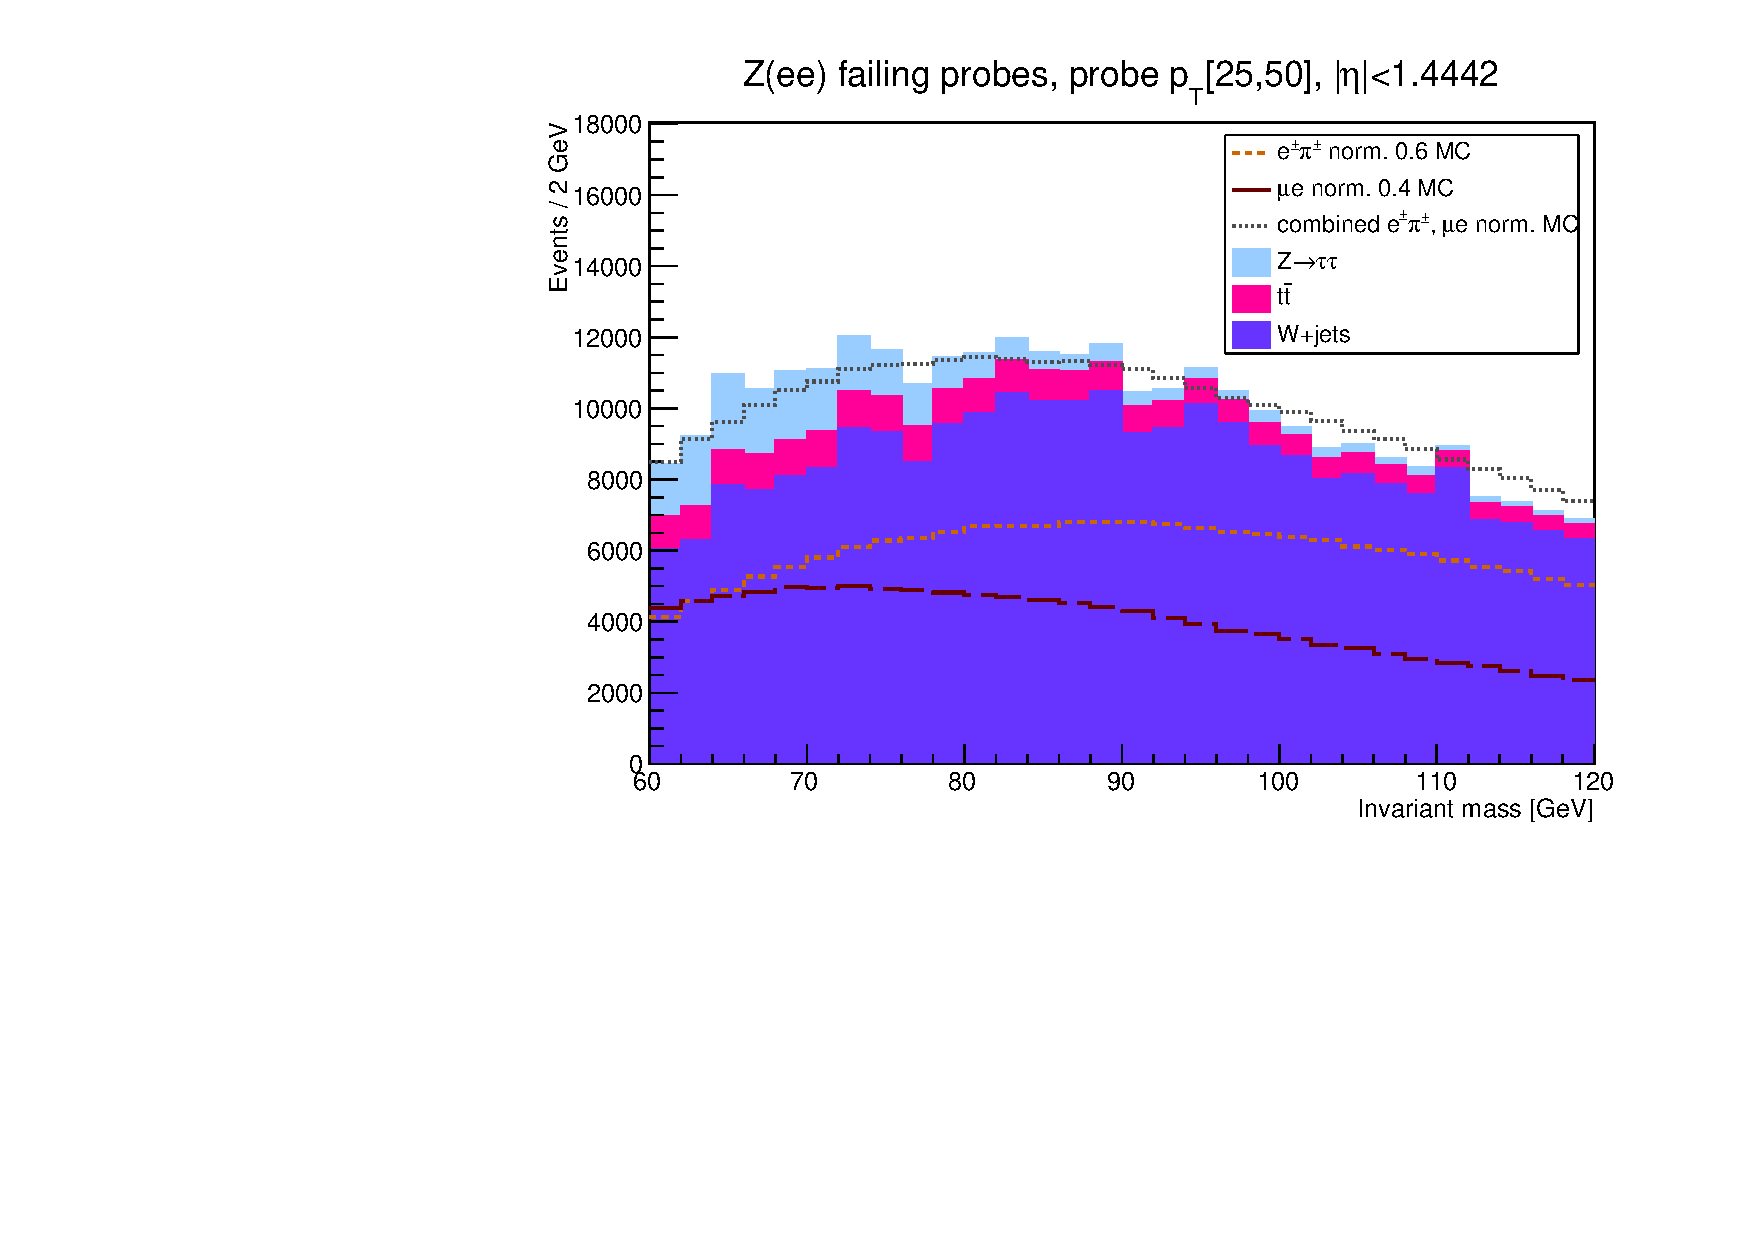
\includegraphics[width=0.75\textwidth]{figures/ZeeEPiEMu.pdf}
	\caption{Simulation of the true background shape, compared with the shapes of the \ensuremath{\ell^{\pm}\pi^{\pm}} selection, the \ensuremath{e\mu} selection, and a linear combination of the two.
    The background is normalized to the integrated luminosity of the 2016 dataset.}
	\label{fig:ZeeEPiEMu}
\end{figure}
\section{Fitting techniques}
\label{sec:tnpfits}
The data efficiency is determined by performing a combined signal plus background fit to each of the
passing and failing categories, in each of the bins of kinematic phase space. 
The efficiency extraction fit provides the number of signal Z events in the passing and failing categories 
by measuring the relative contribution of signal and background.
The nominal values for the signal and background yields in data are fit using a signal hypothesis
of truth-matched Drell-Yan Monte Carlo templates (as described in Section~\ref{sec:tnpsel}),
convoluted with a Gaussian resolution function which allows for widening and shifting of the
simulated peak position. The background hypothesis is a fixed shape derived from data, as
described in Section~\ref{sec:tnpcontrol}.
In the dielectron fits, the relative contribution of \ensuremath{e^{\pm}\pi^{\pm}} versus 
{\ensuremath{e\mu} data is a free parameter in the fit.

The binning choice for the probe leptons is the following:
\begin{itemize}
\item Probe electron $\pt$: $\{$10, 15, 20, 25, 30, 35, 40, 42, 44, 46, 48, 50, 55, 60, 70, 100$\}$ $\GeV$;
\item Probe electron $\eta$: $\{$-2.5, -2.4, -2.3, -2.2, -2.1, -2.0, -1.8, -1.566, -1.4442, -1.2, -1, -0.8, -0.6, -0.4, -0.2, 0, 0.2, 0.4, 0.6, 0.8, 1, 1.2, 1.4442, 1.566, 1.8, 2.0, 2.1, 2.2, 2.3, 2.4, 2.5$\}$;
\item Probe muon $\pt$: $\{$10, 15, 20, 25, 30, 35, 40, 45, 50, 55, 60, 120$\}$ $\GeV$;
\item Probe muon $\eta$: $\{$-2.4, -2.1, -1.6, -1.2, -0.9, -0.3, -0.2, 0.2, 0.3, 0.9, 1.2, 1.6, 2.1, 2.4$\}$;
\end{itemize}

Representing the phase space bin and the pass/fail category with the index $i$,
the number of signal events $N_{sig}^{i}$ (and associated statistical uncertainty) in this bin
is calculated as the total number of data events $N_{total}^{i}$ (Poisson distributed),
minus the estimated background yield $N_{bkg}^{i}$
(with statistical uncertainty from the negative likelihood minimization procedure).
Then, in each phase space bin, the efficiency is determined as
\begin{align*}
  \varepsilon = \frac{N_{sig}^{pass}}{N_{sig}^{pass}+N_{sig}^{fail}}
\end{align*}
and the statistical errors are propagated conservatively assuming zero, not negative
correlation between the passing and failing signal yields.

Examples of the nominal efficiency extraction fits for dimuons are shown in Figures~\ref{fig:ZmmNominalFits1} and~\ref{fig:ZmmNominalFits2}.
Similar examples for dielectrons are shown in Figures~\ref{fig:ZeeNominalFits1} and~\ref{fig:ZeeNominalFits2}.
In order to assess the goodness-of-fit, we compute a modified $\chi^2$ test which accounts for
statistical uncertainties in the data as well as the MC signal template, as shown in the plots.

The MC efficiency is determined by counting the normalized yields of the passing and failing templates described above.
\begin{figure}
\centering
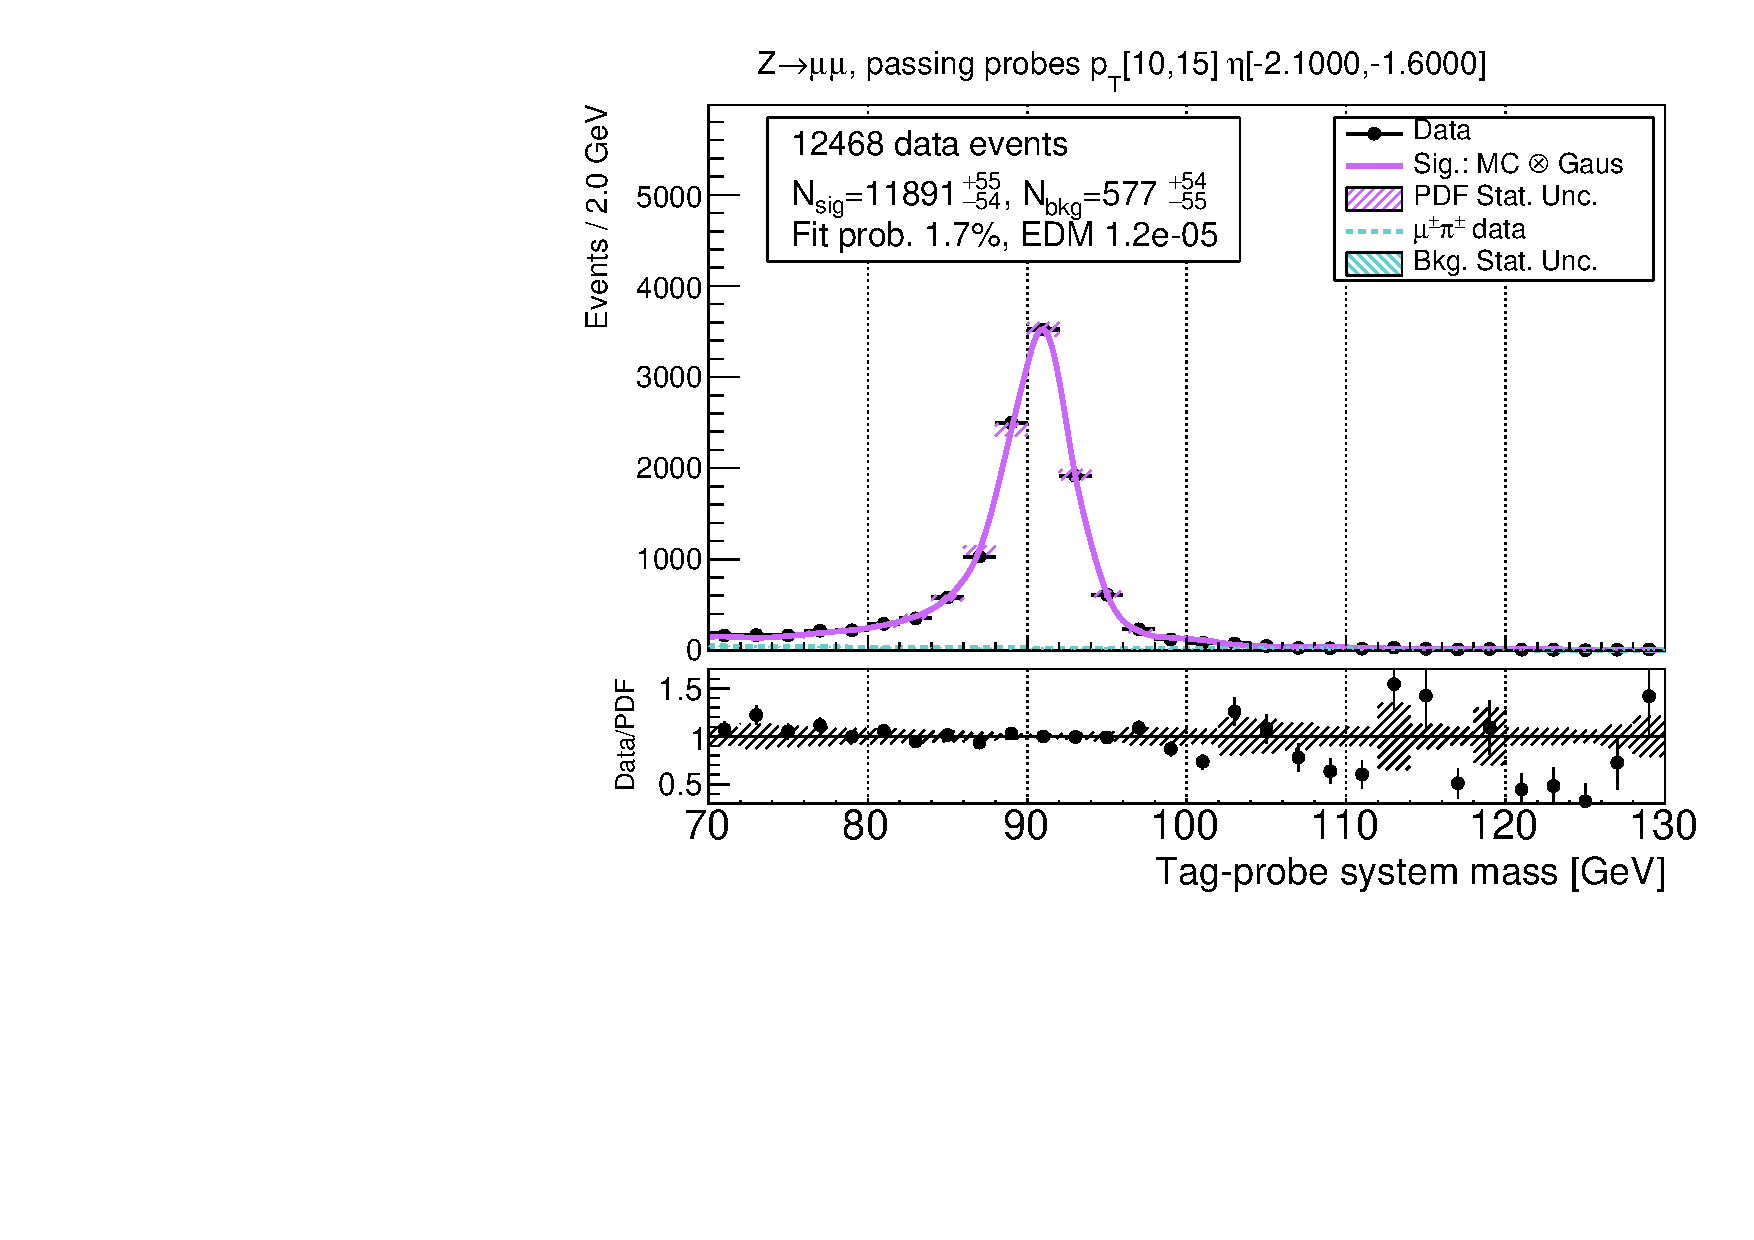
\includegraphics[width=0.49\textwidth]{figures/Zmm_RecoTemplate_BkgLPi_pass_ptBin0_etaBin1.pdf}
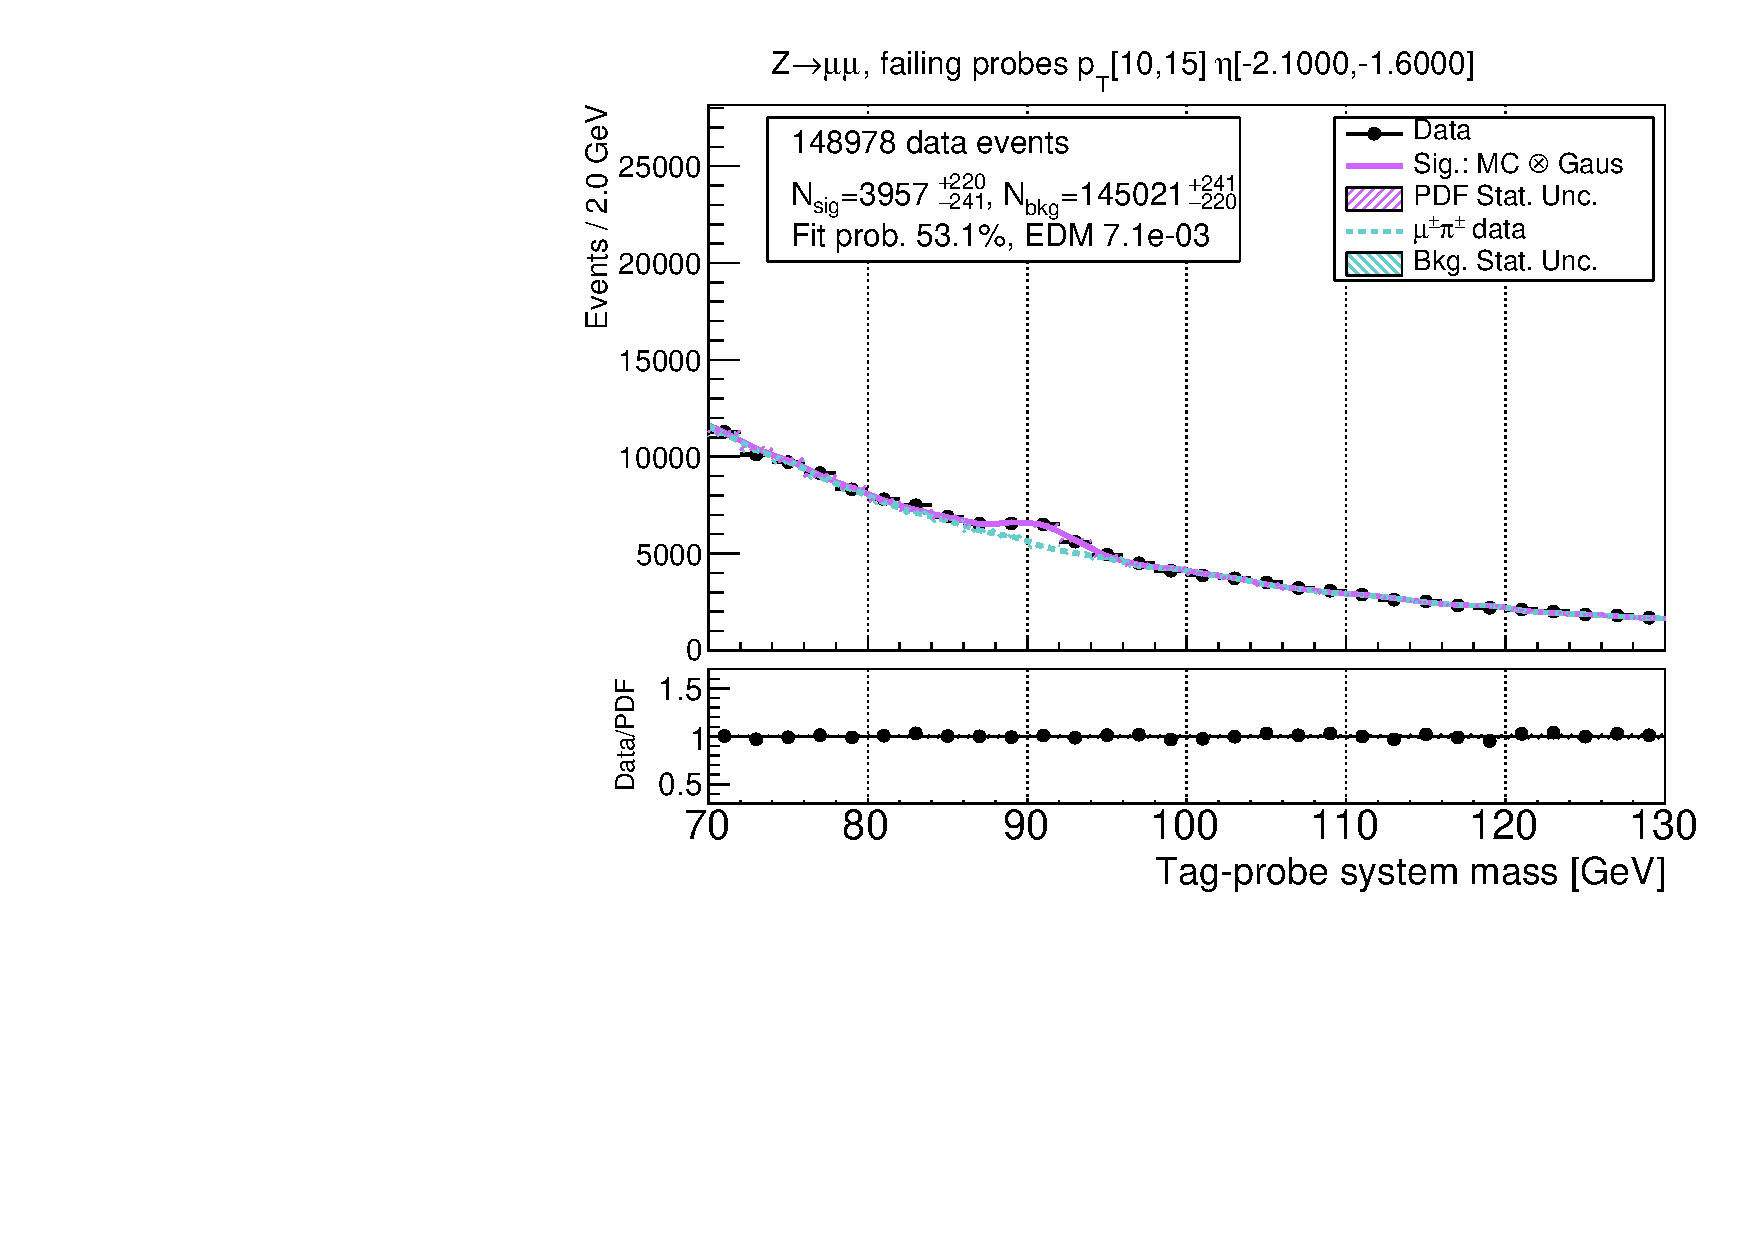
\includegraphics[width=0.49\textwidth]{figures/Zmm_RecoTemplate_BkgLPi_fail_ptBin0_etaBin1.pdf}
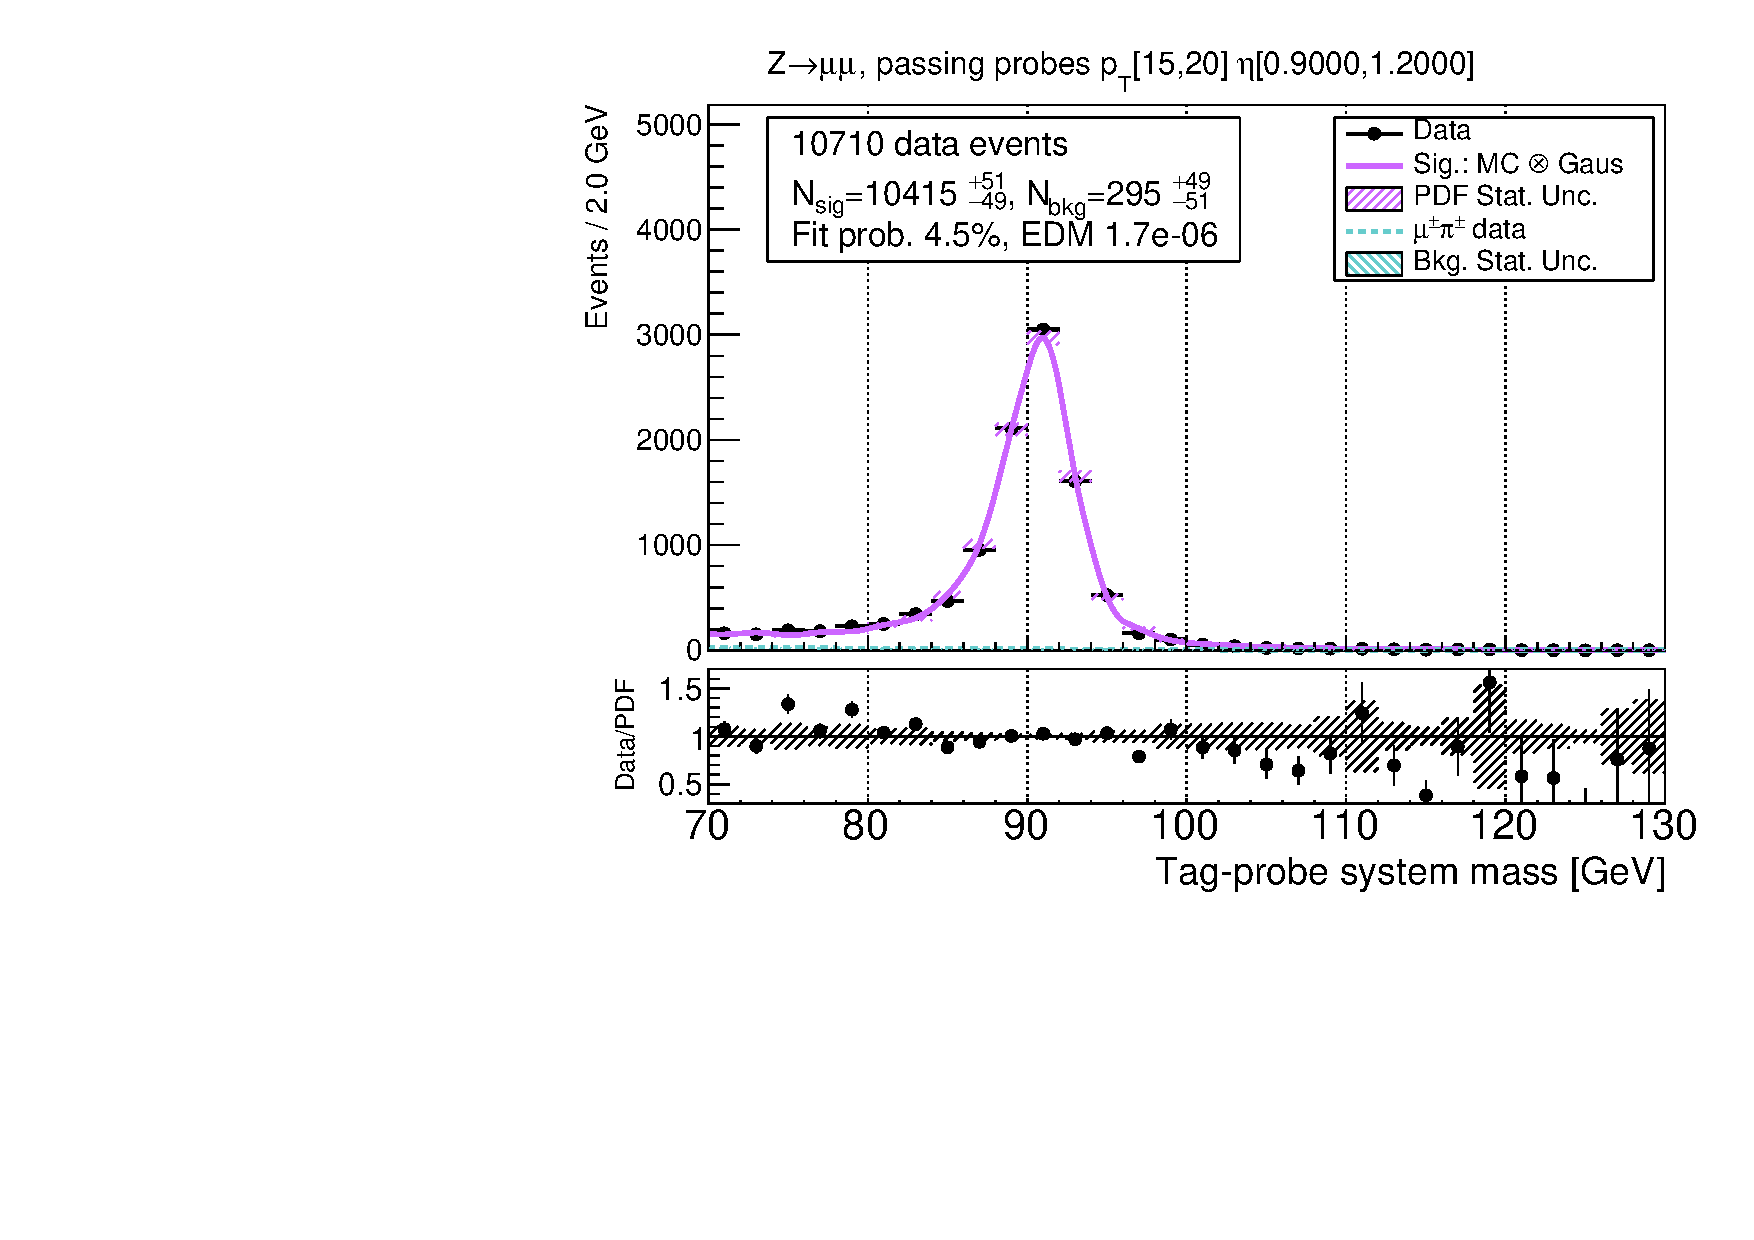
\includegraphics[width=0.49\textwidth]{figures/Zmm_RecoTemplate_BkgLPi_pass_ptBin1_etaBin9.pdf}
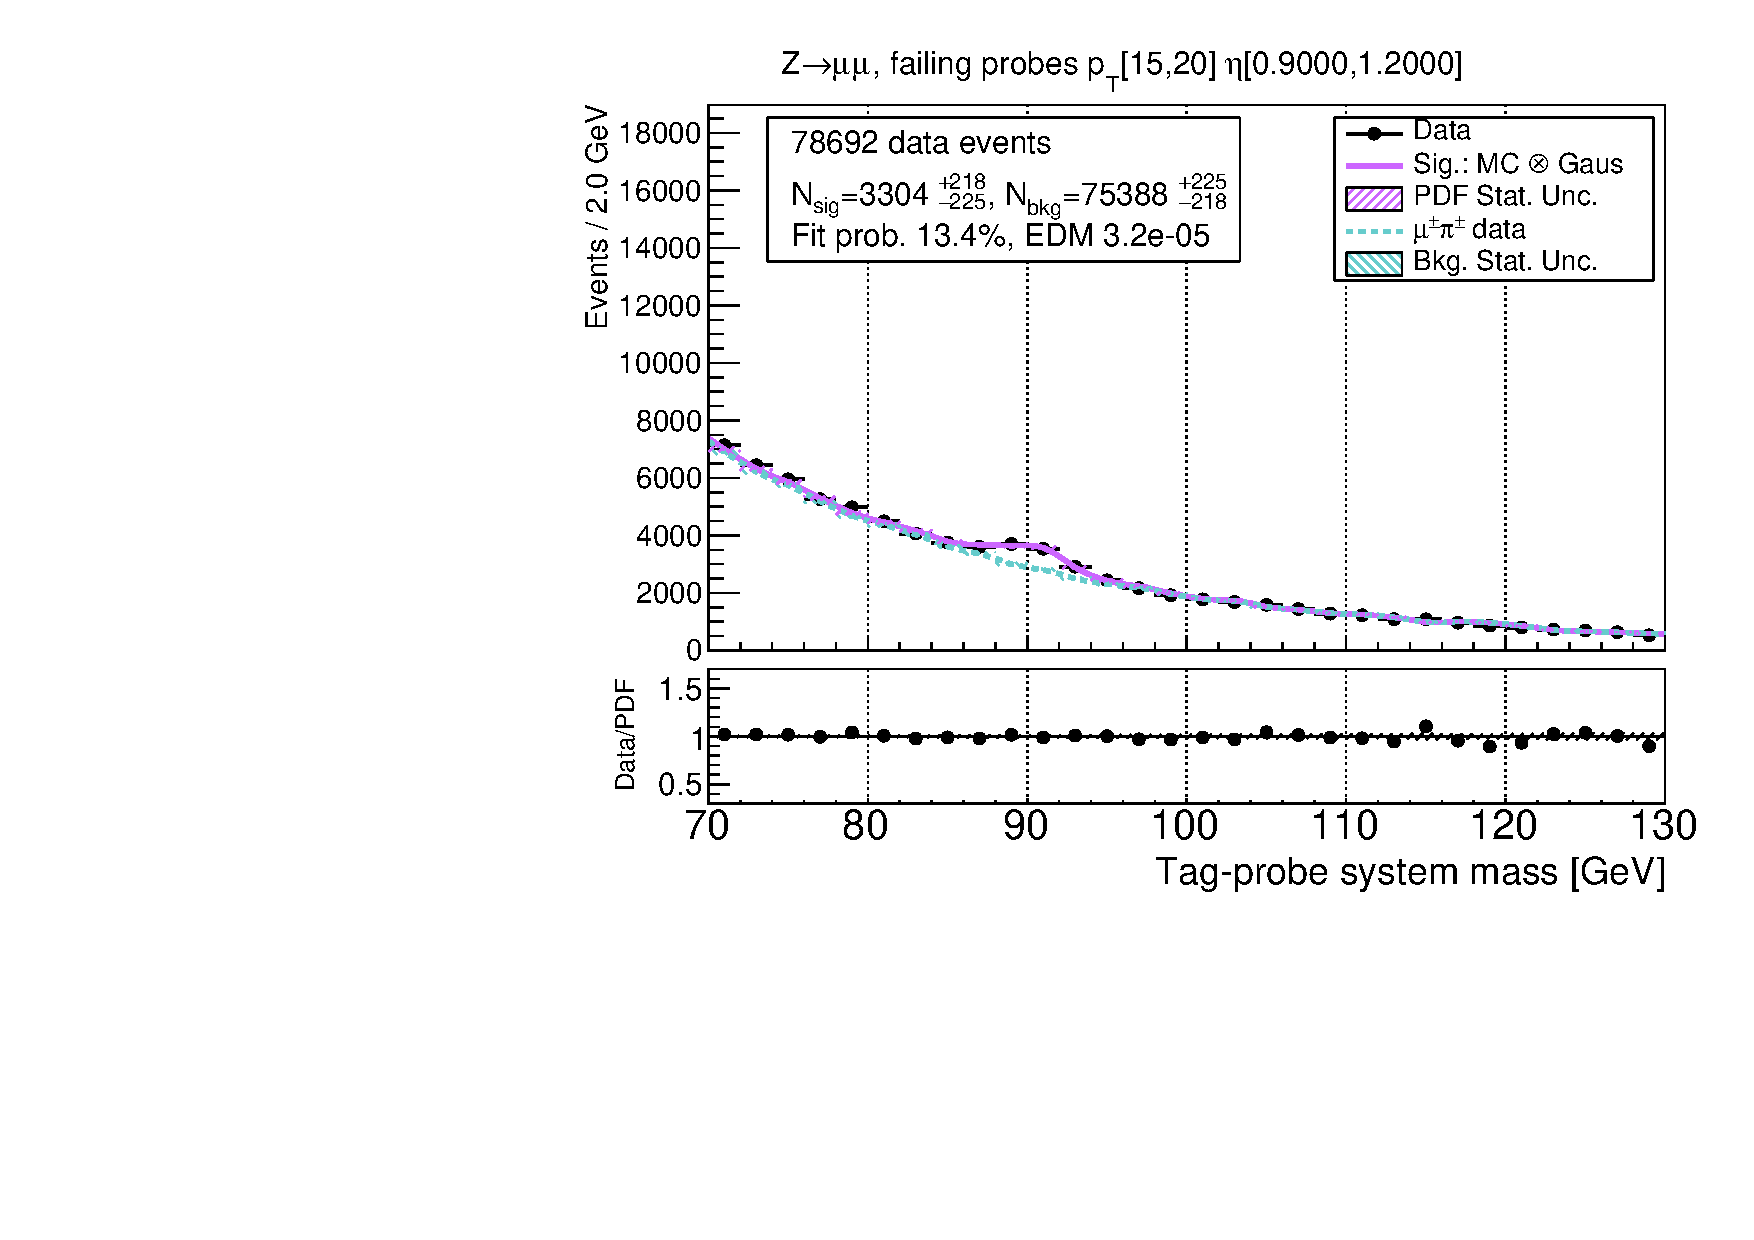
\includegraphics[width=0.49\textwidth]{figures/Zmm_RecoTemplate_BkgLPi_fail_ptBin1_etaBin9.pdf}
\caption{Efficiency extraction fits for the Medium muon working point using the data-driven background shape, at low muon transverse momentum.}
\label{fig:ZmmNominalFits1}
\end{figure}
\begin{figure}
\centering
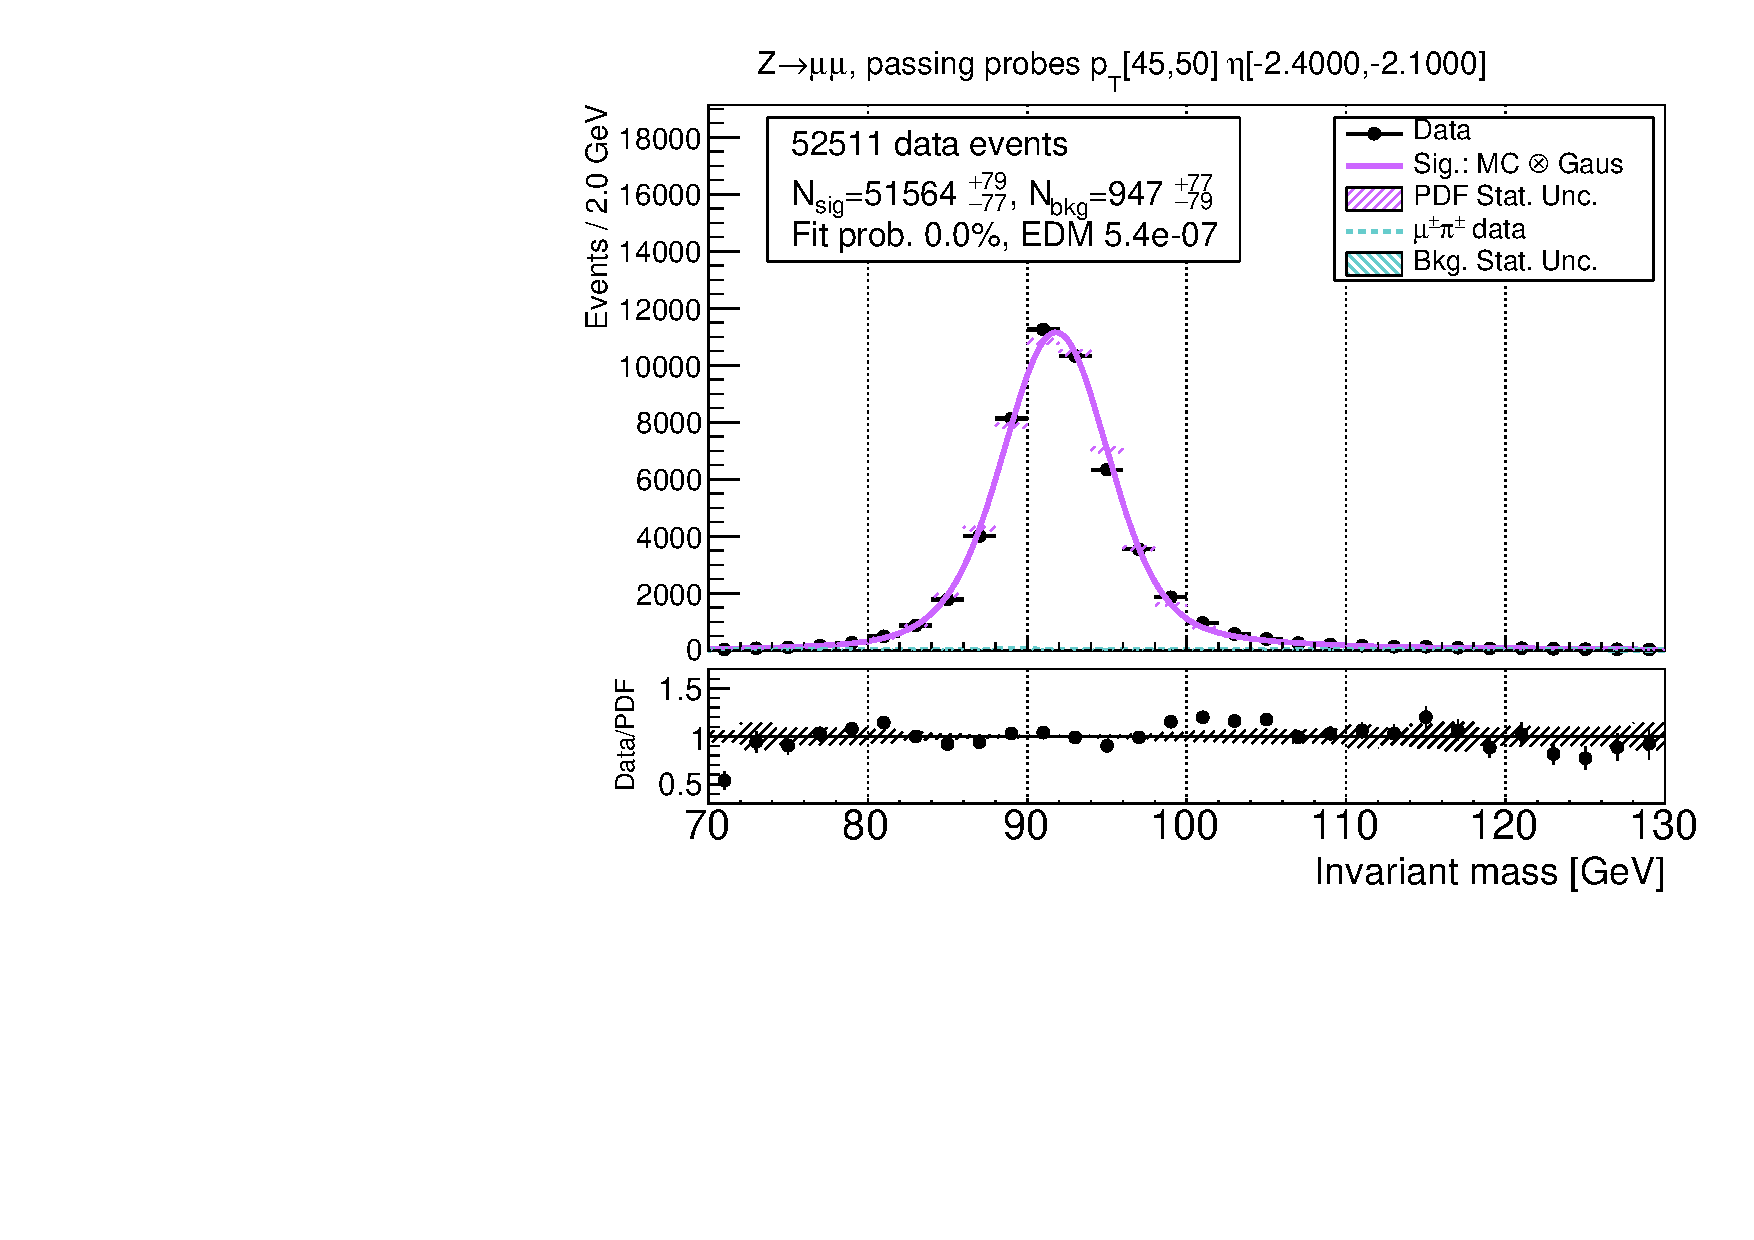
\includegraphics[width=0.49\textwidth]{figures/Zmm_RecoTemplate_BkgLPi_pass_ptBin7_etaBin0.pdf}
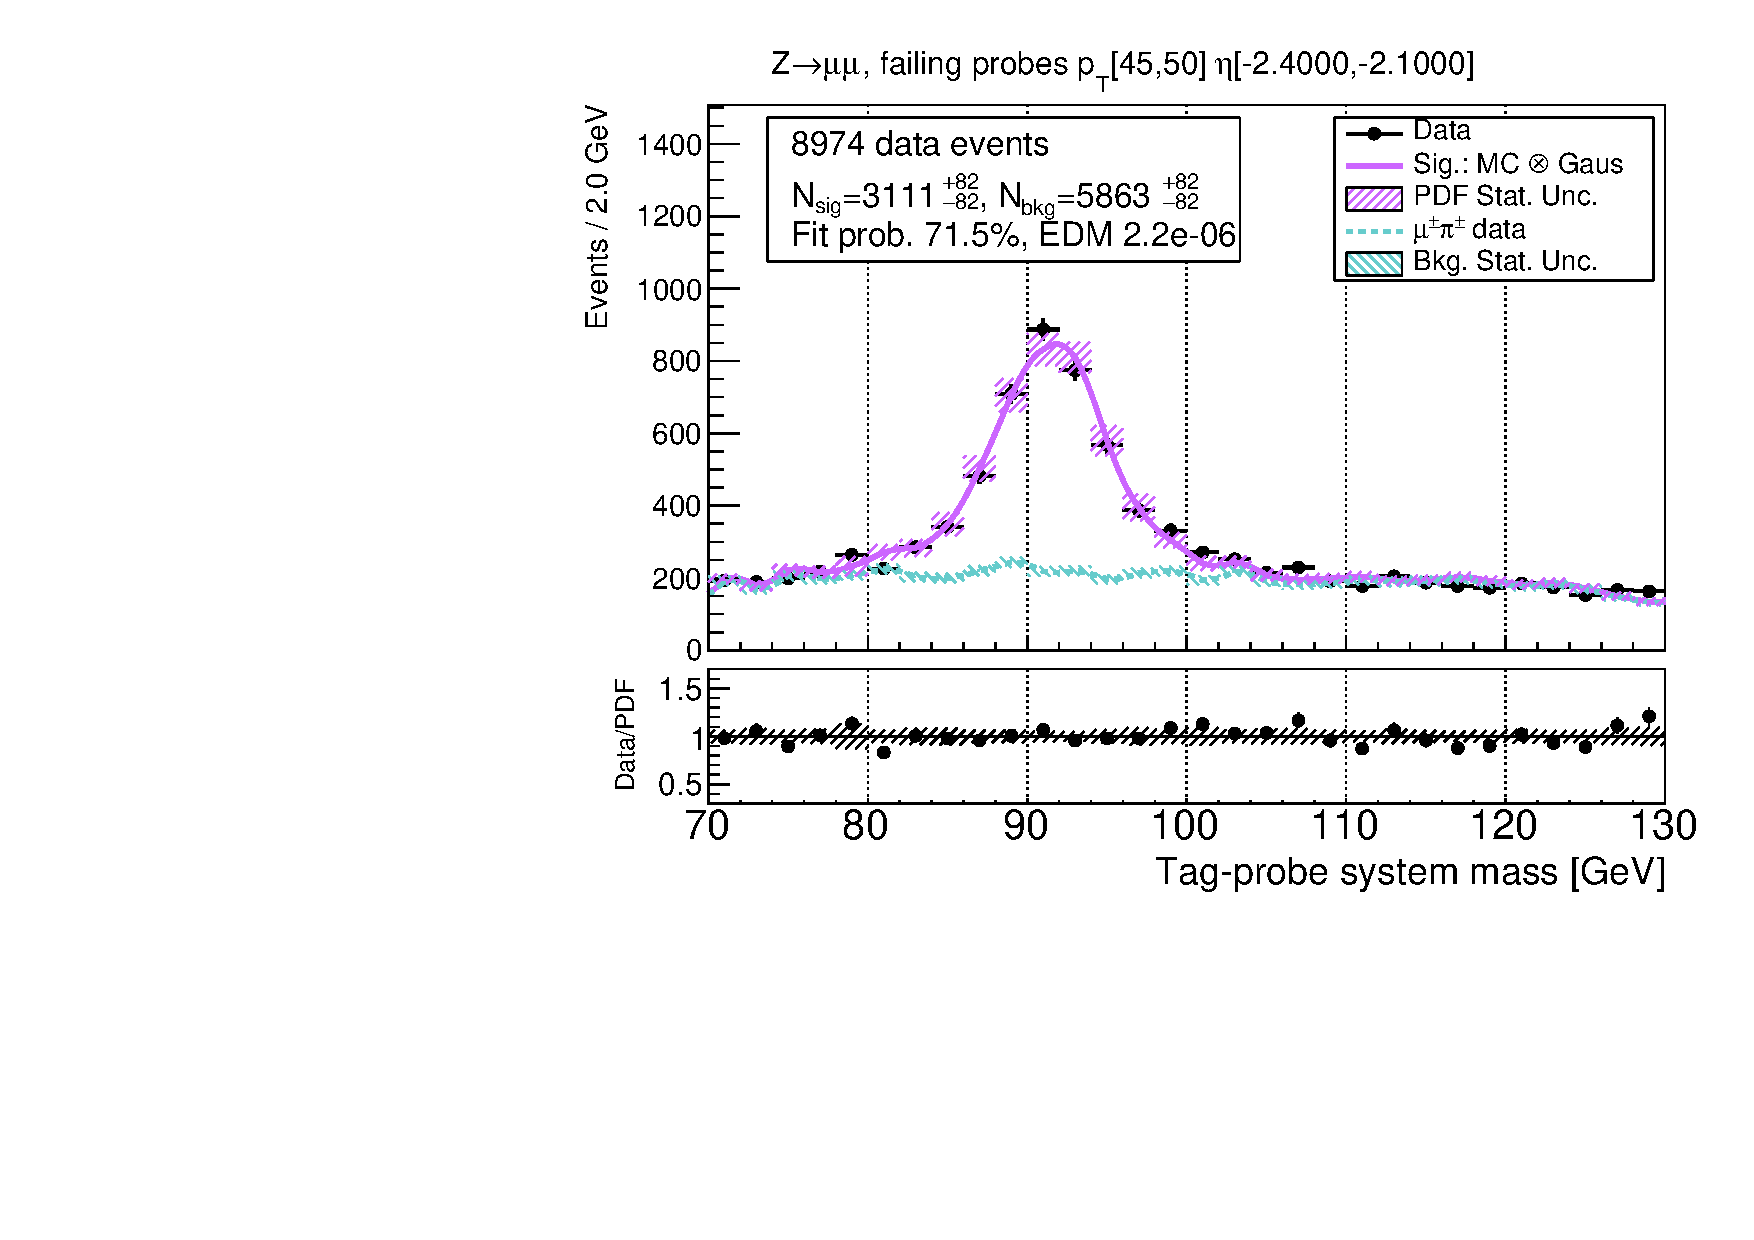
\includegraphics[width=0.49\textwidth]{figures/Zmm_RecoTemplate_BkgLPi_fail_ptBin7_etaBin0.pdf}
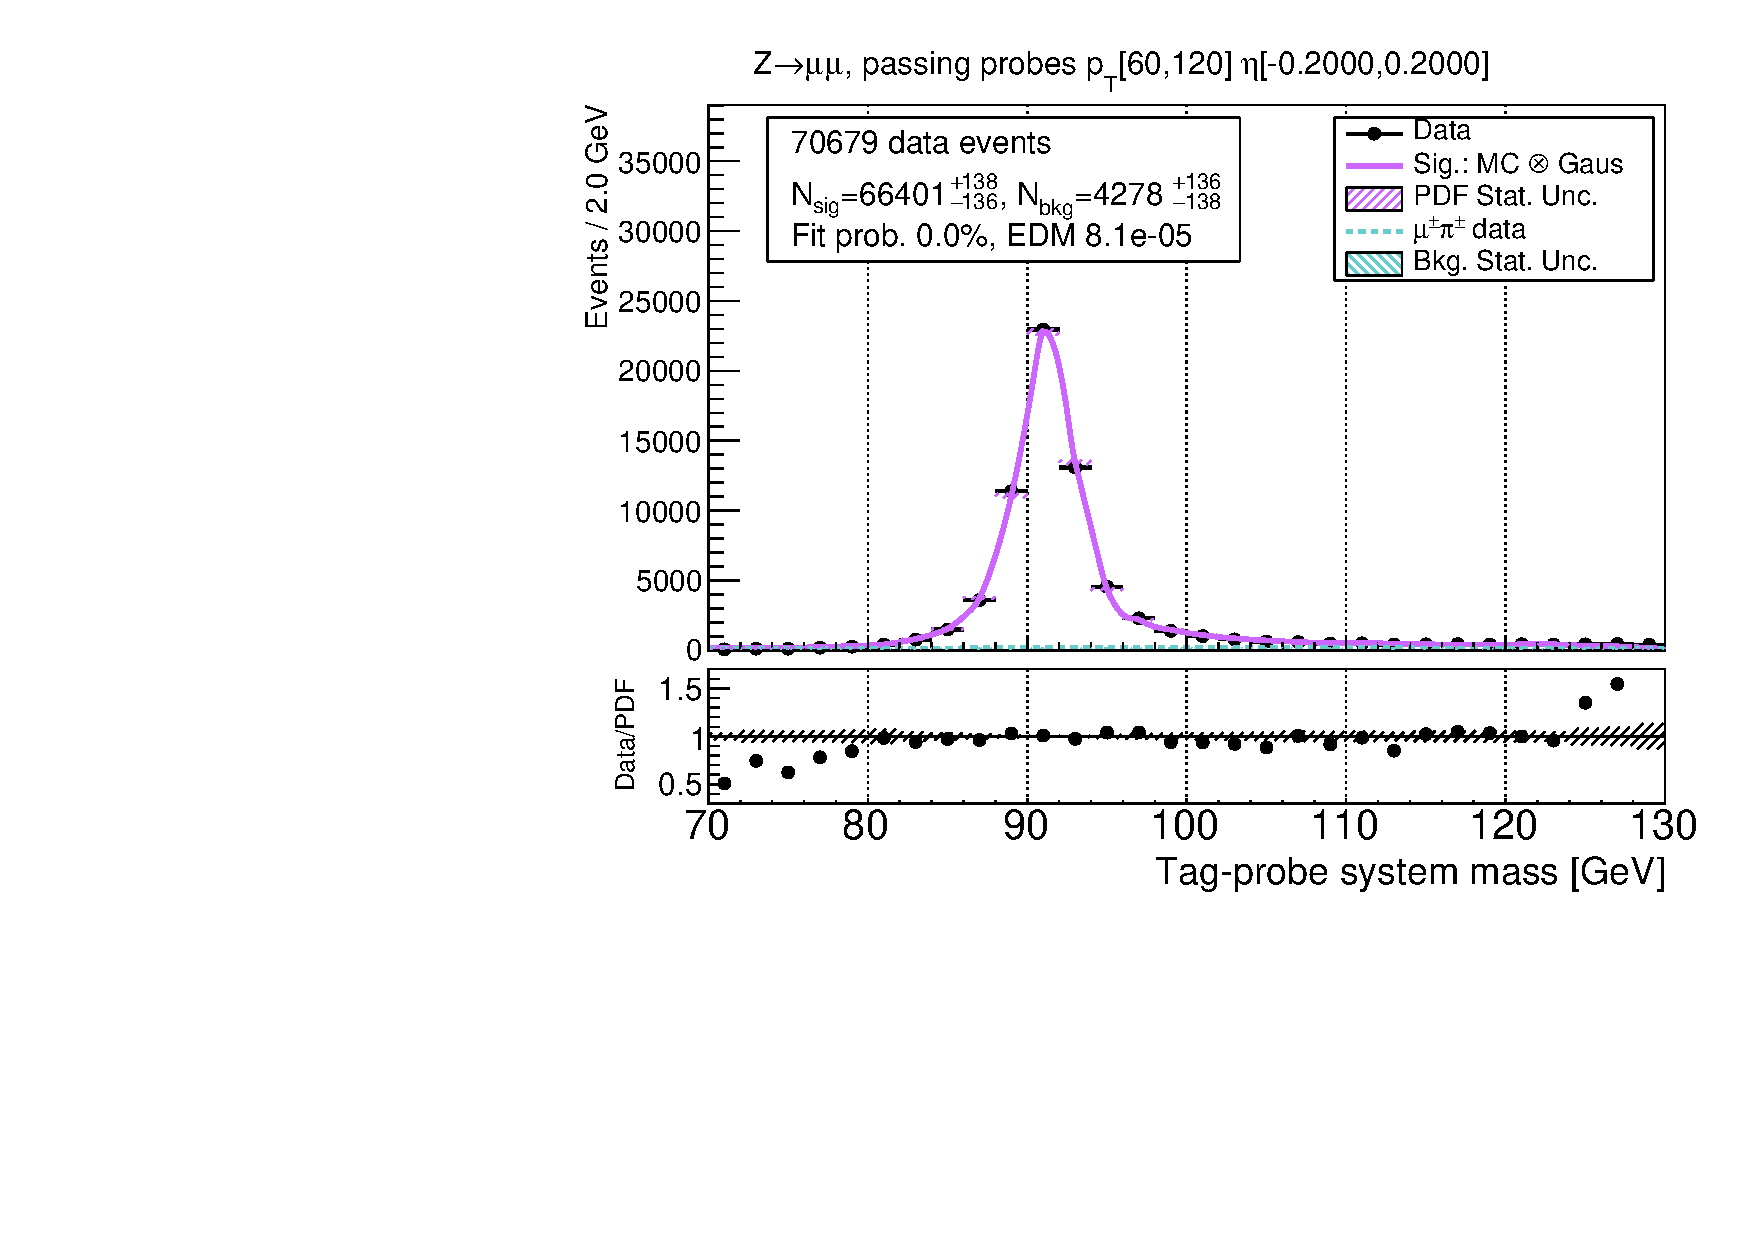
\includegraphics[width=0.49\textwidth]{figures/Zmm_RecoTemplate_BkgLPi_pass_ptBin10_etaBin6.pdf}
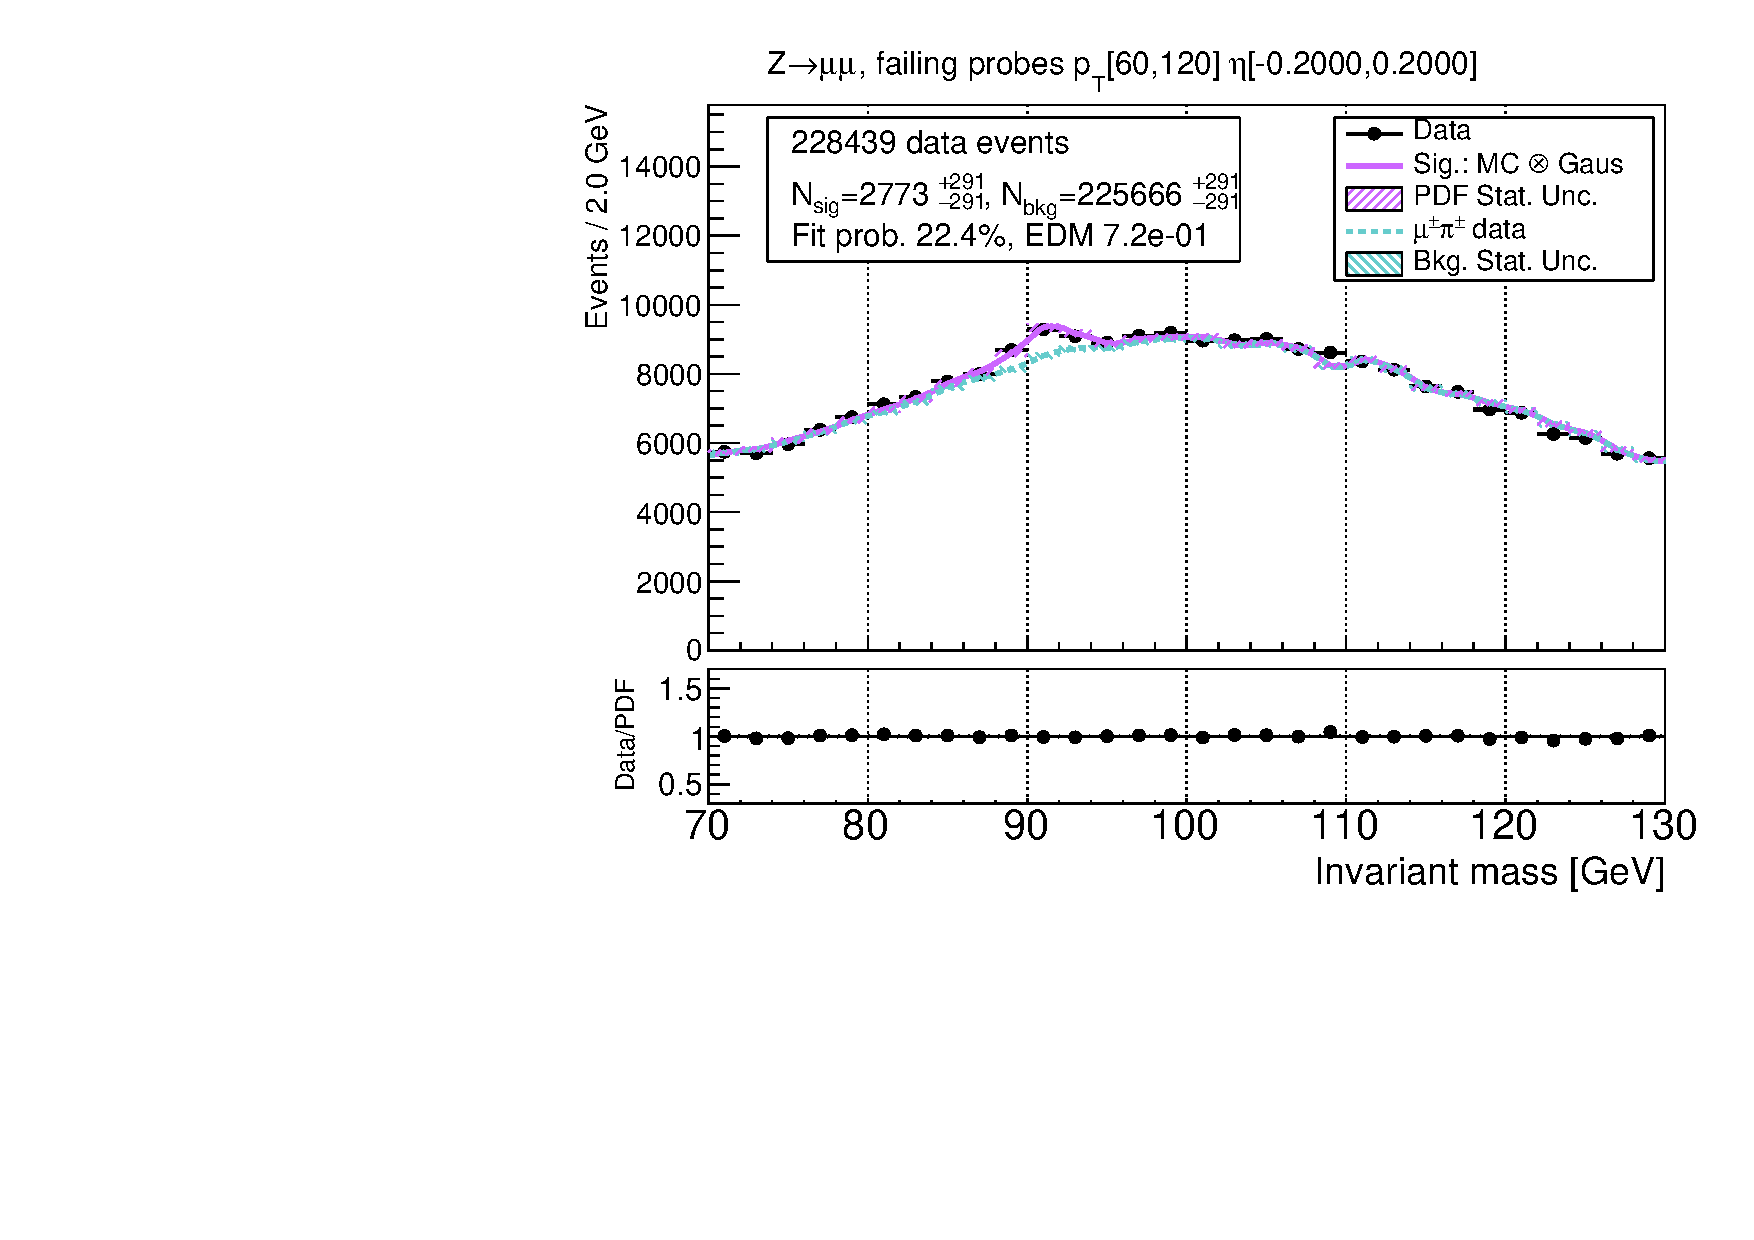
\includegraphics[width=0.49\textwidth]{figures/Zmm_RecoTemplate_BkgLPi_fail_ptBin10_etaBin6.pdf}
\caption{Efficiency extraction fits for the Medium muon working point using the data-driven background shape, at higher values of muon transverse momentum.}
\label{fig:ZmmNominalFits2}
\end{figure}

\begin{figure}
\centering
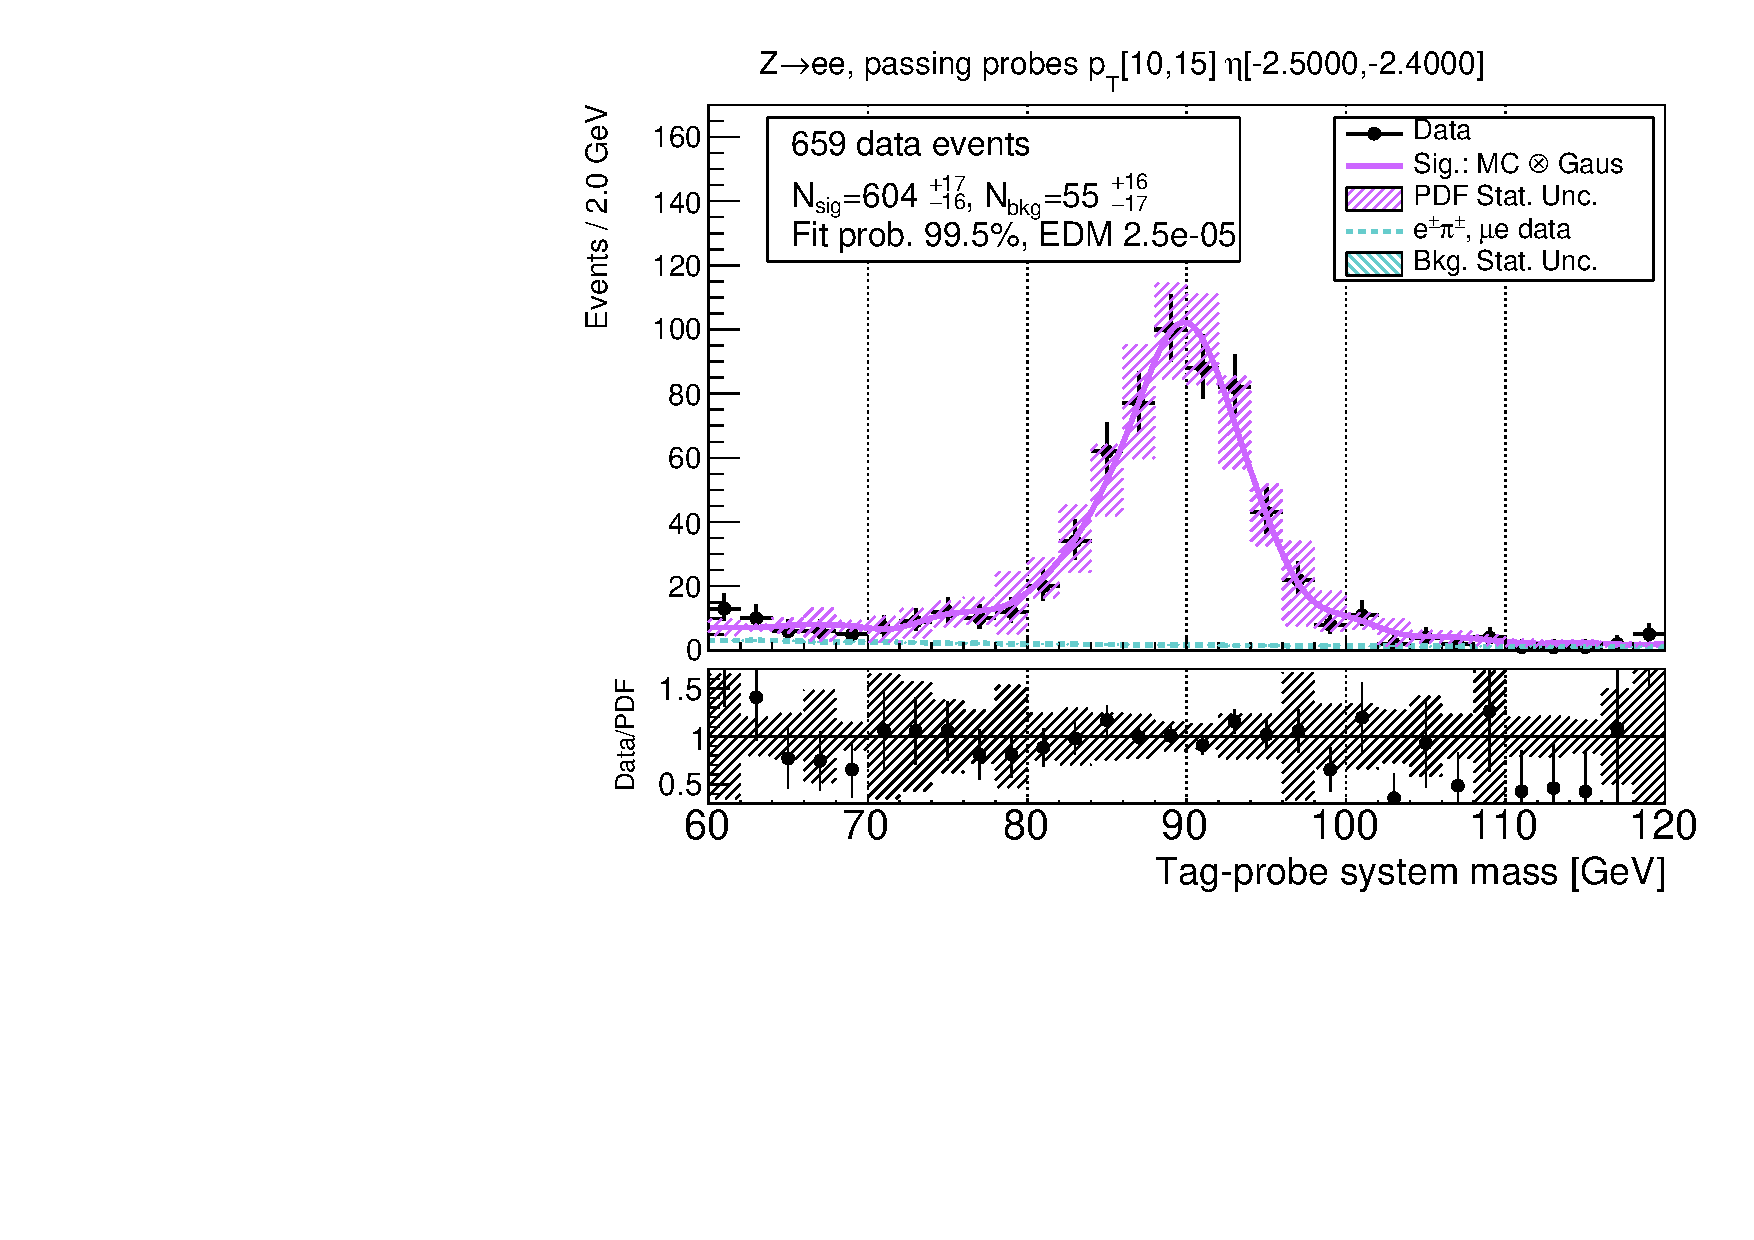
\includegraphics[width=0.49\textwidth]{figures/Zee_RecoTemplate_BkgLPiEMu_pass_ptBin0_etaBin0.pdf}
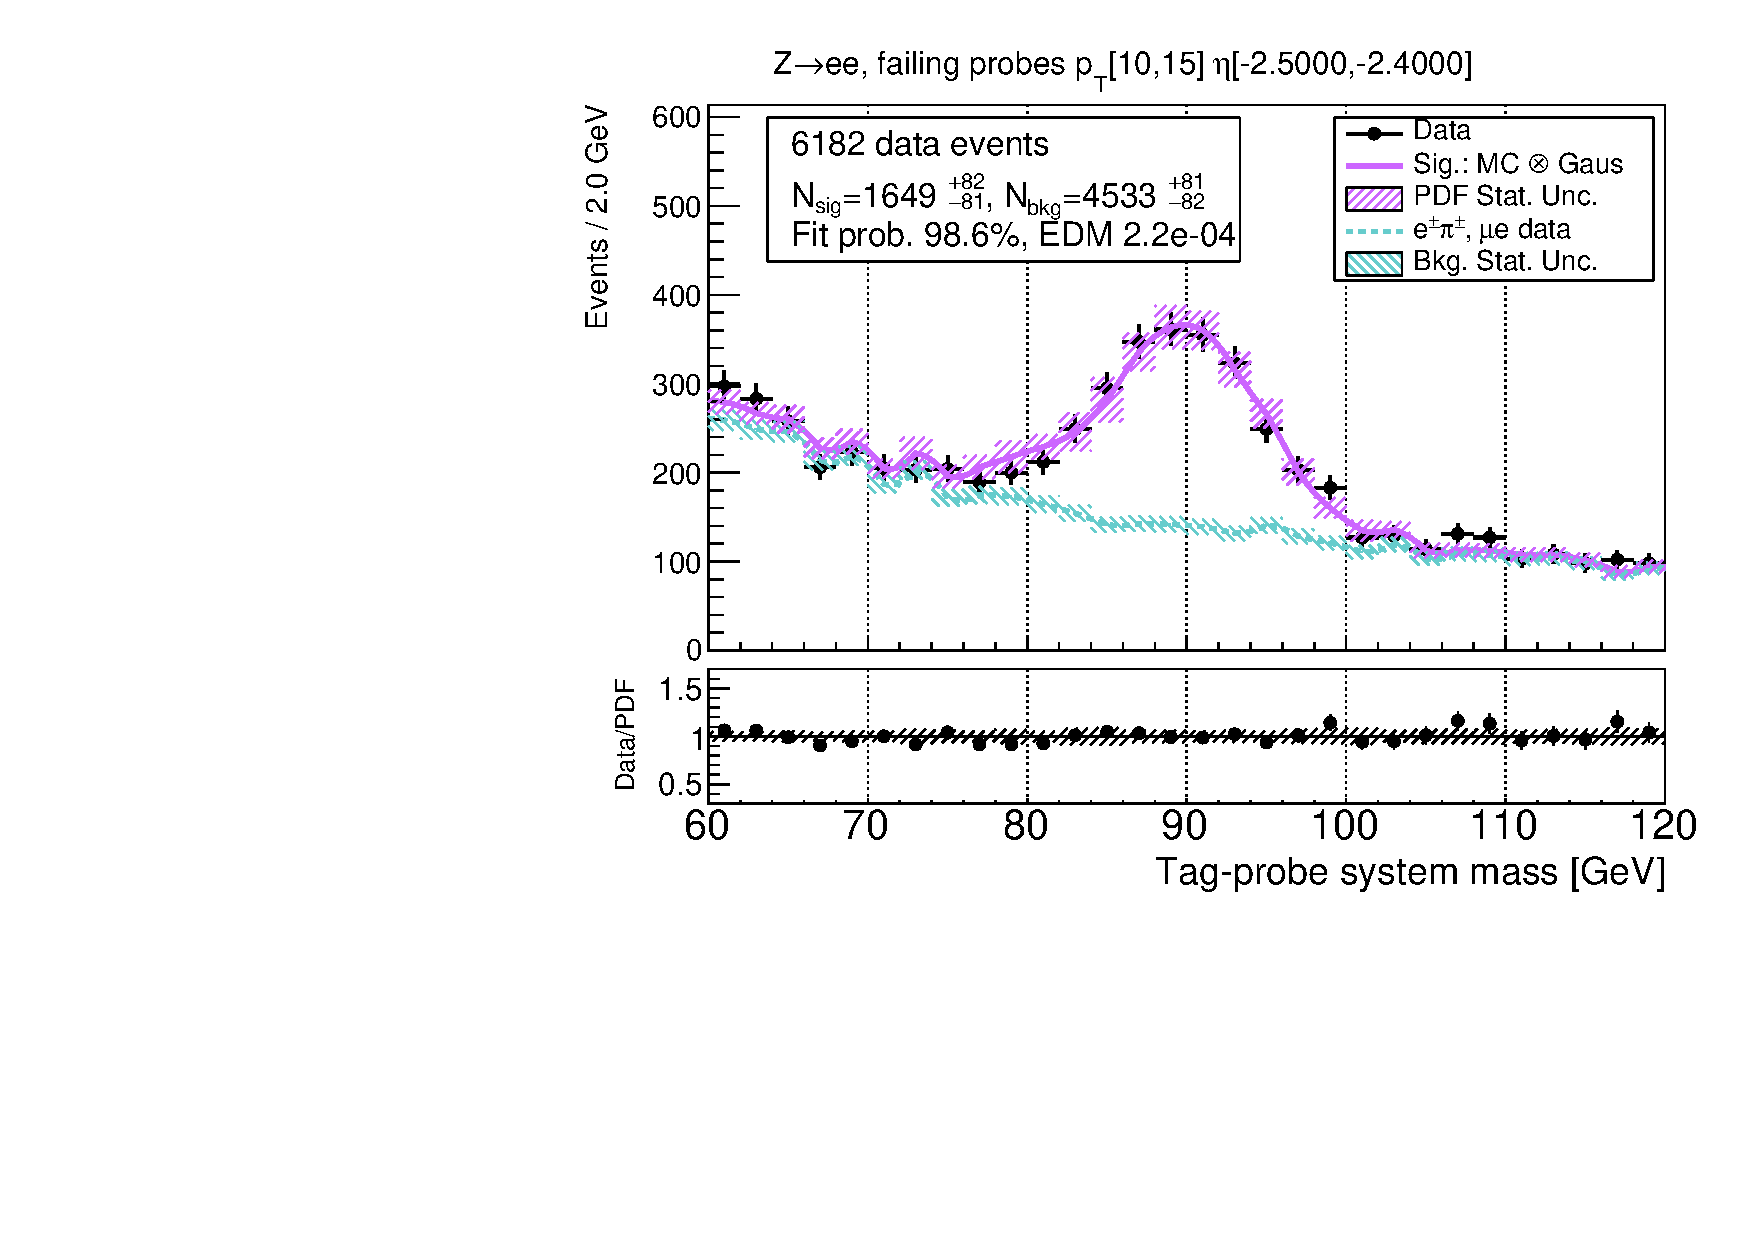
\includegraphics[width=0.49\textwidth]{figures/Zee_RecoTemplate_BkgLPiEMu_fail_ptBin0_etaBin0.pdf}
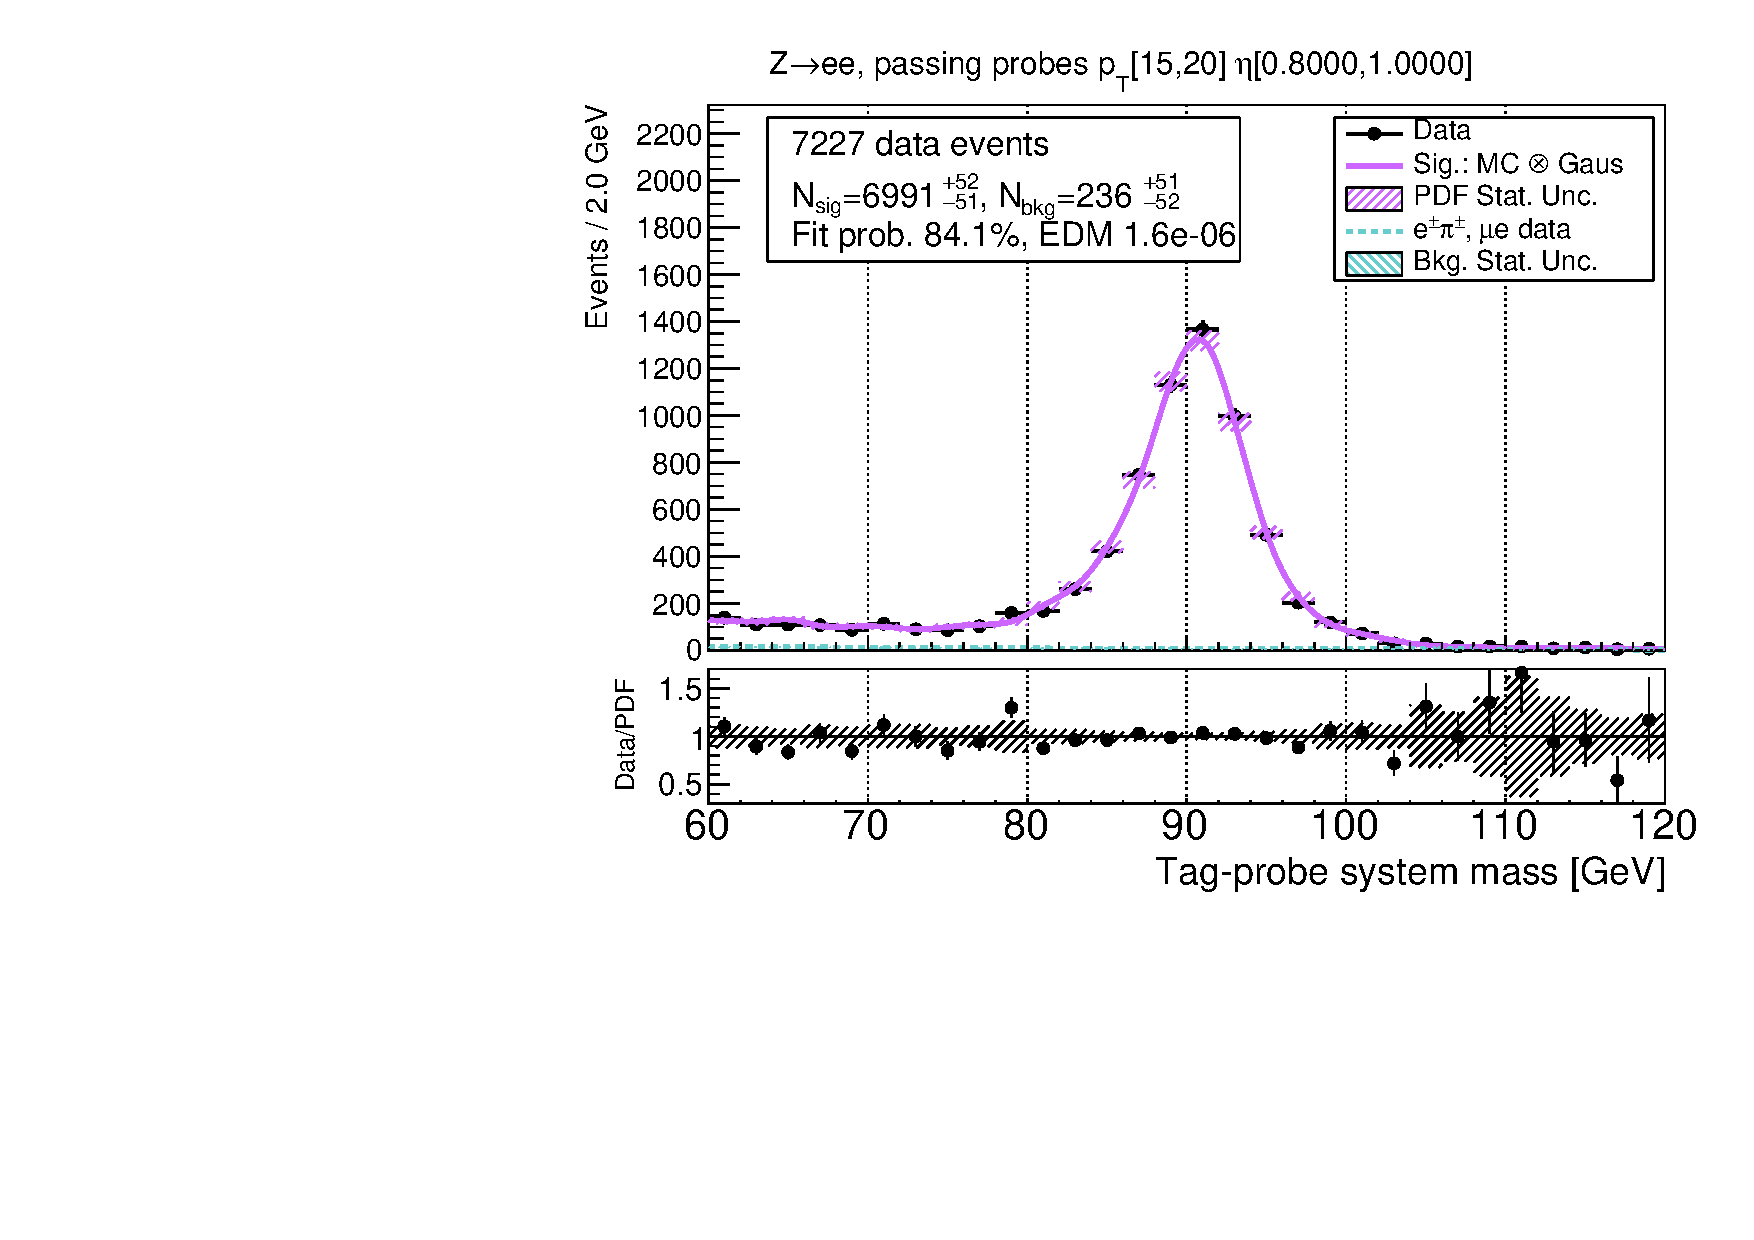
\includegraphics[width=0.49\textwidth]{figures/Zee_RecoTemplate_BkgLPiEMu_pass_ptBin1_etaBin19.pdf}
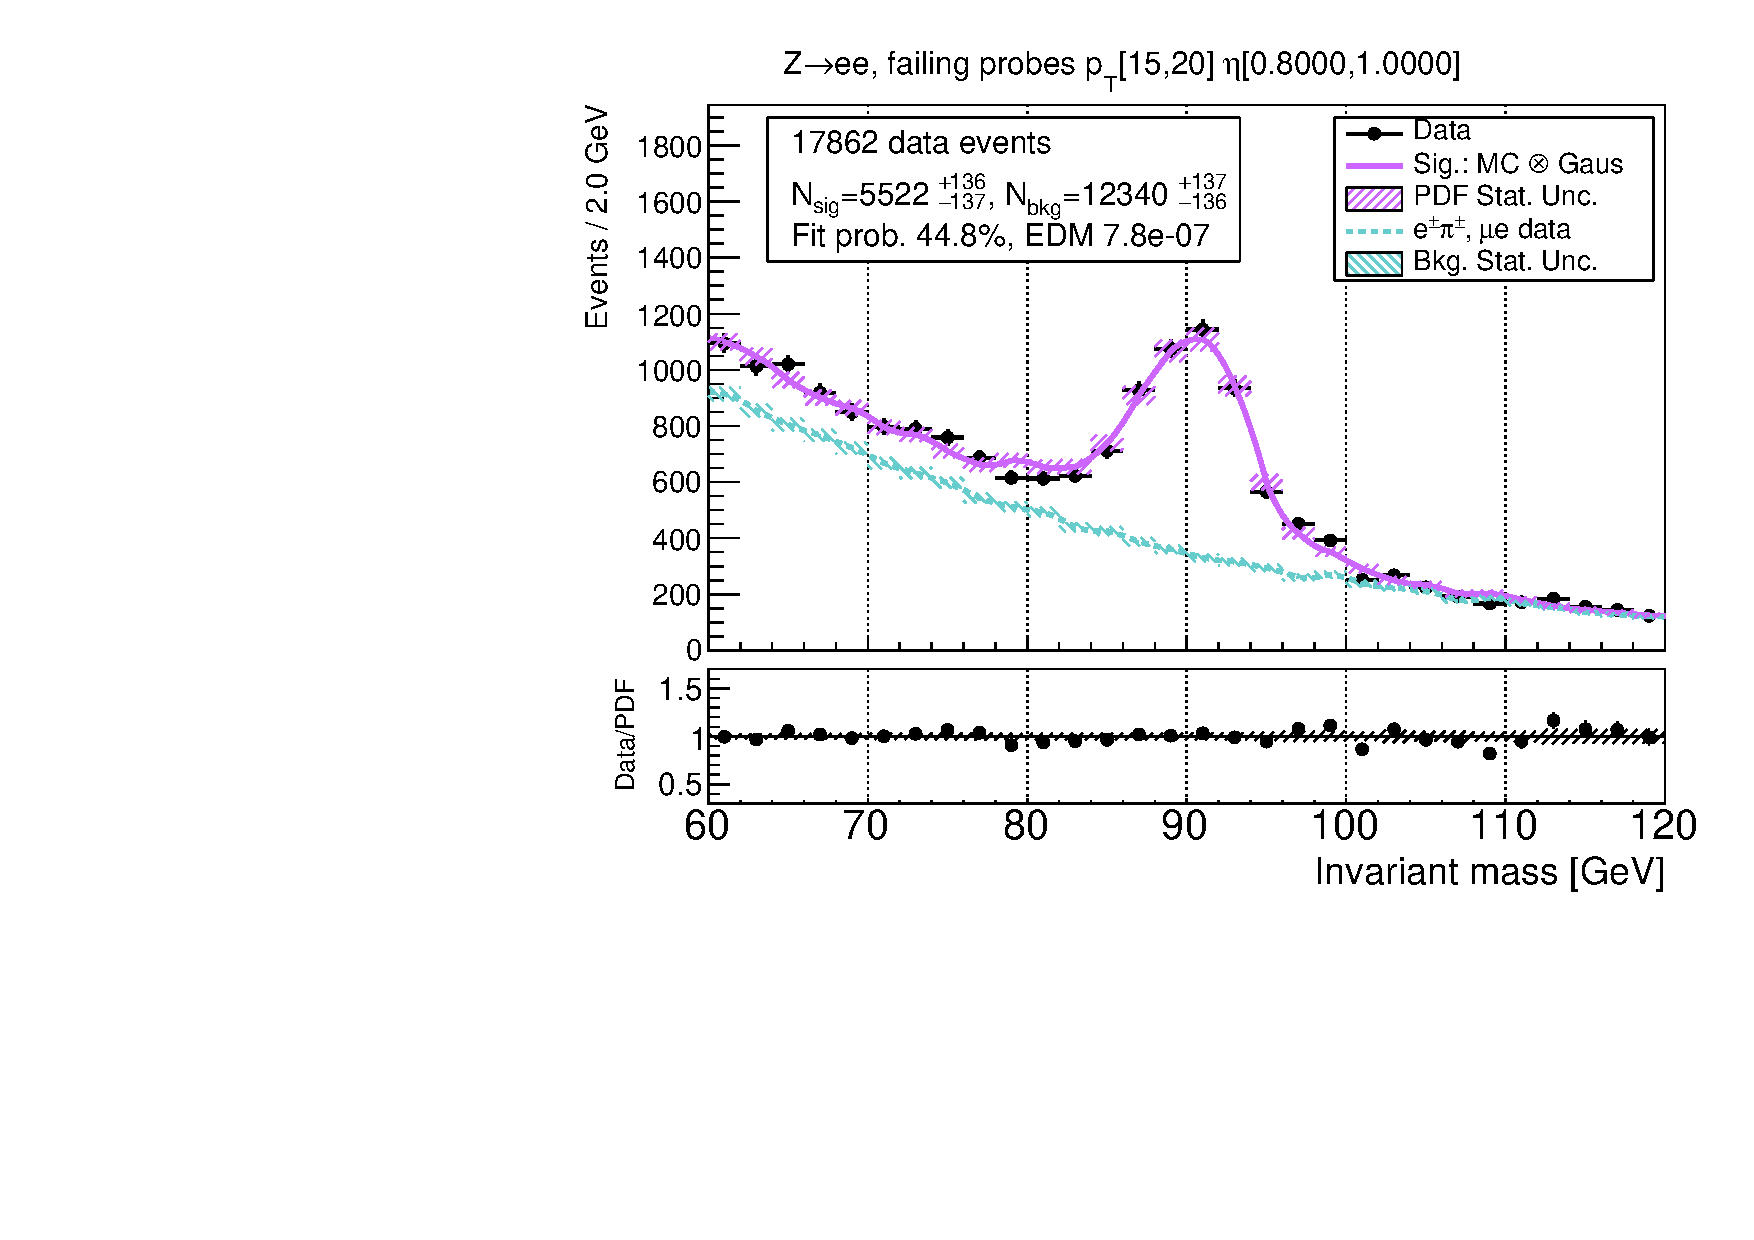
\includegraphics[width=0.49\textwidth]{figures/Zee_RecoTemplate_BkgLPiEMu_fail_ptBin1_etaBin19.pdf}
\caption{Efficiency extraction fits for the Medium electron working point using the data-driven background shape, at low electron transverse momentum.}
\label{fig:ZeeNominalFits1}
\end{figure}
\begin{figure}
\centering
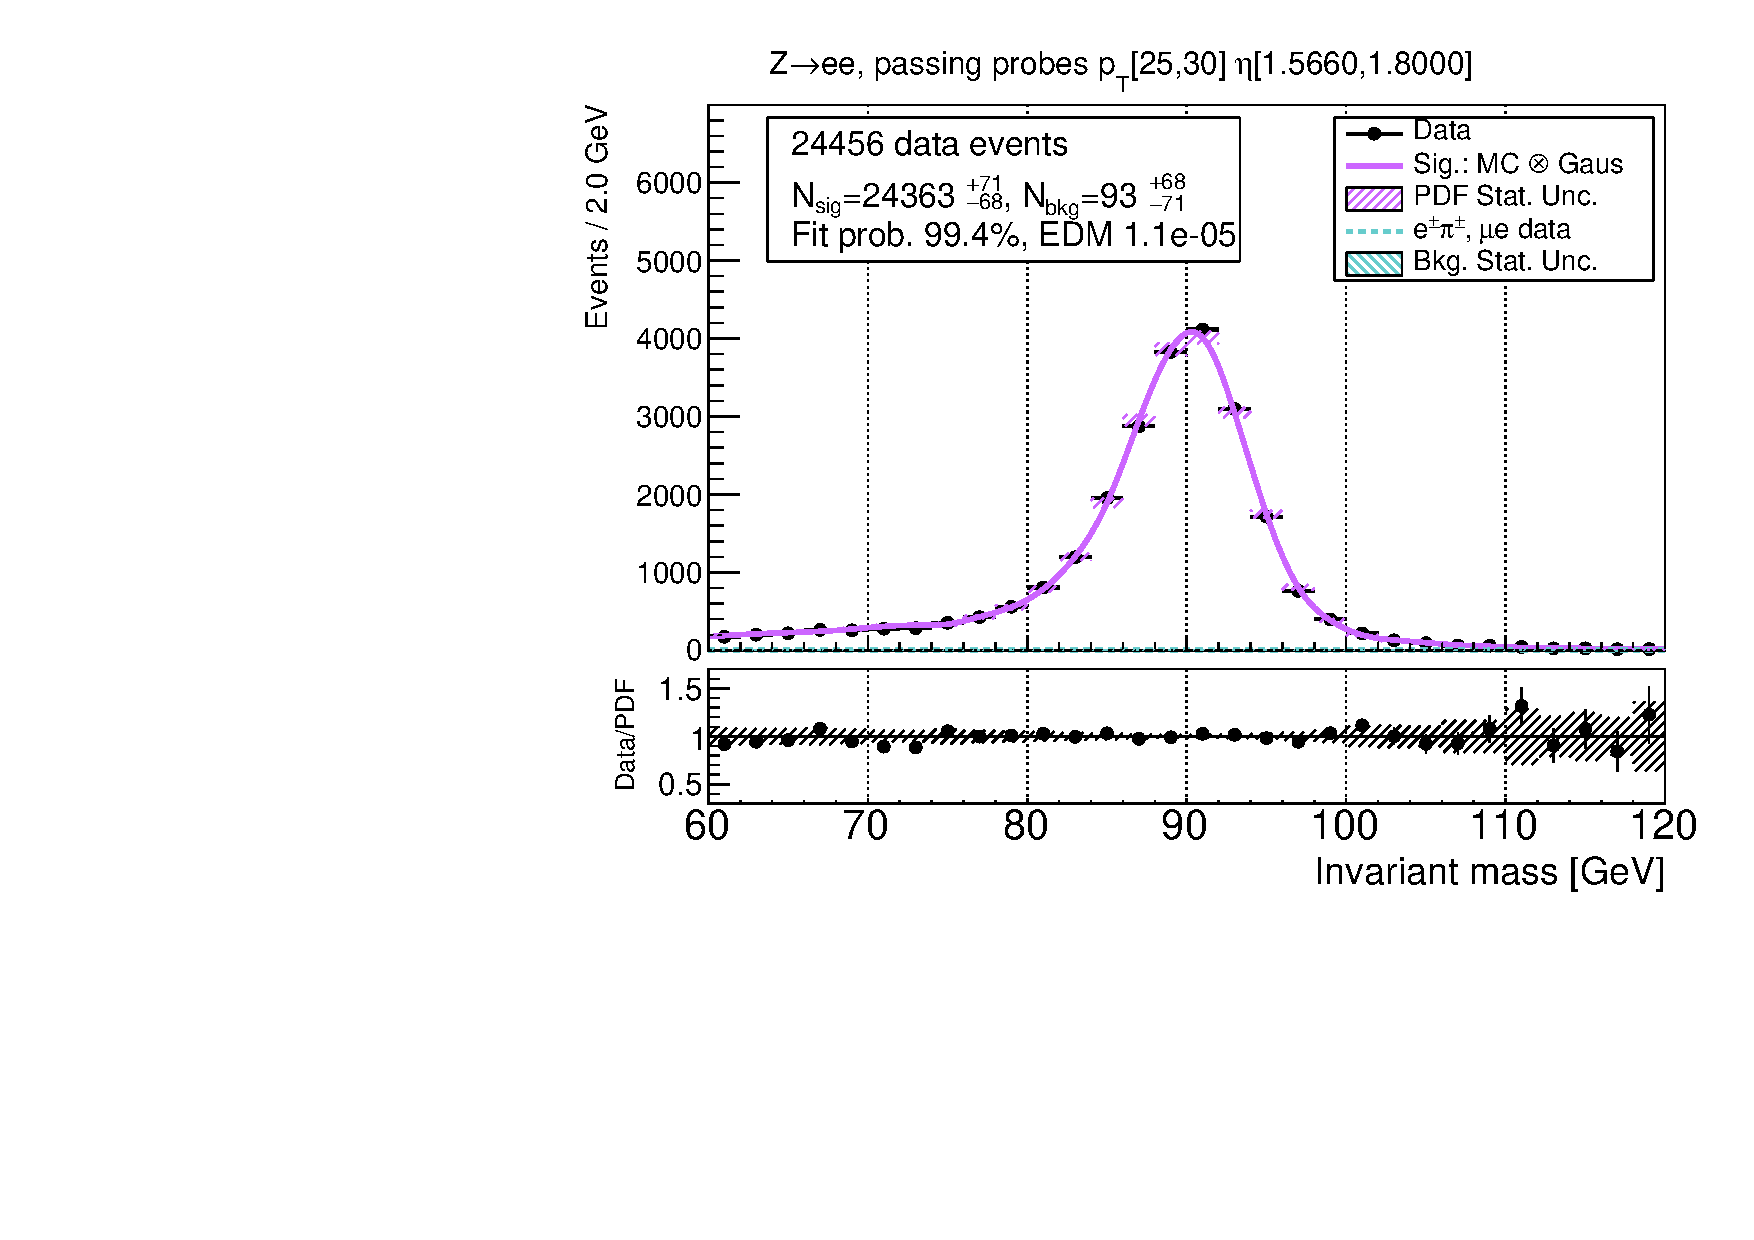
\includegraphics[width=0.49\textwidth]{figures/Zee_RecoTemplate_BkgLPiEMu_pass_ptBin3_etaBin23.pdf}
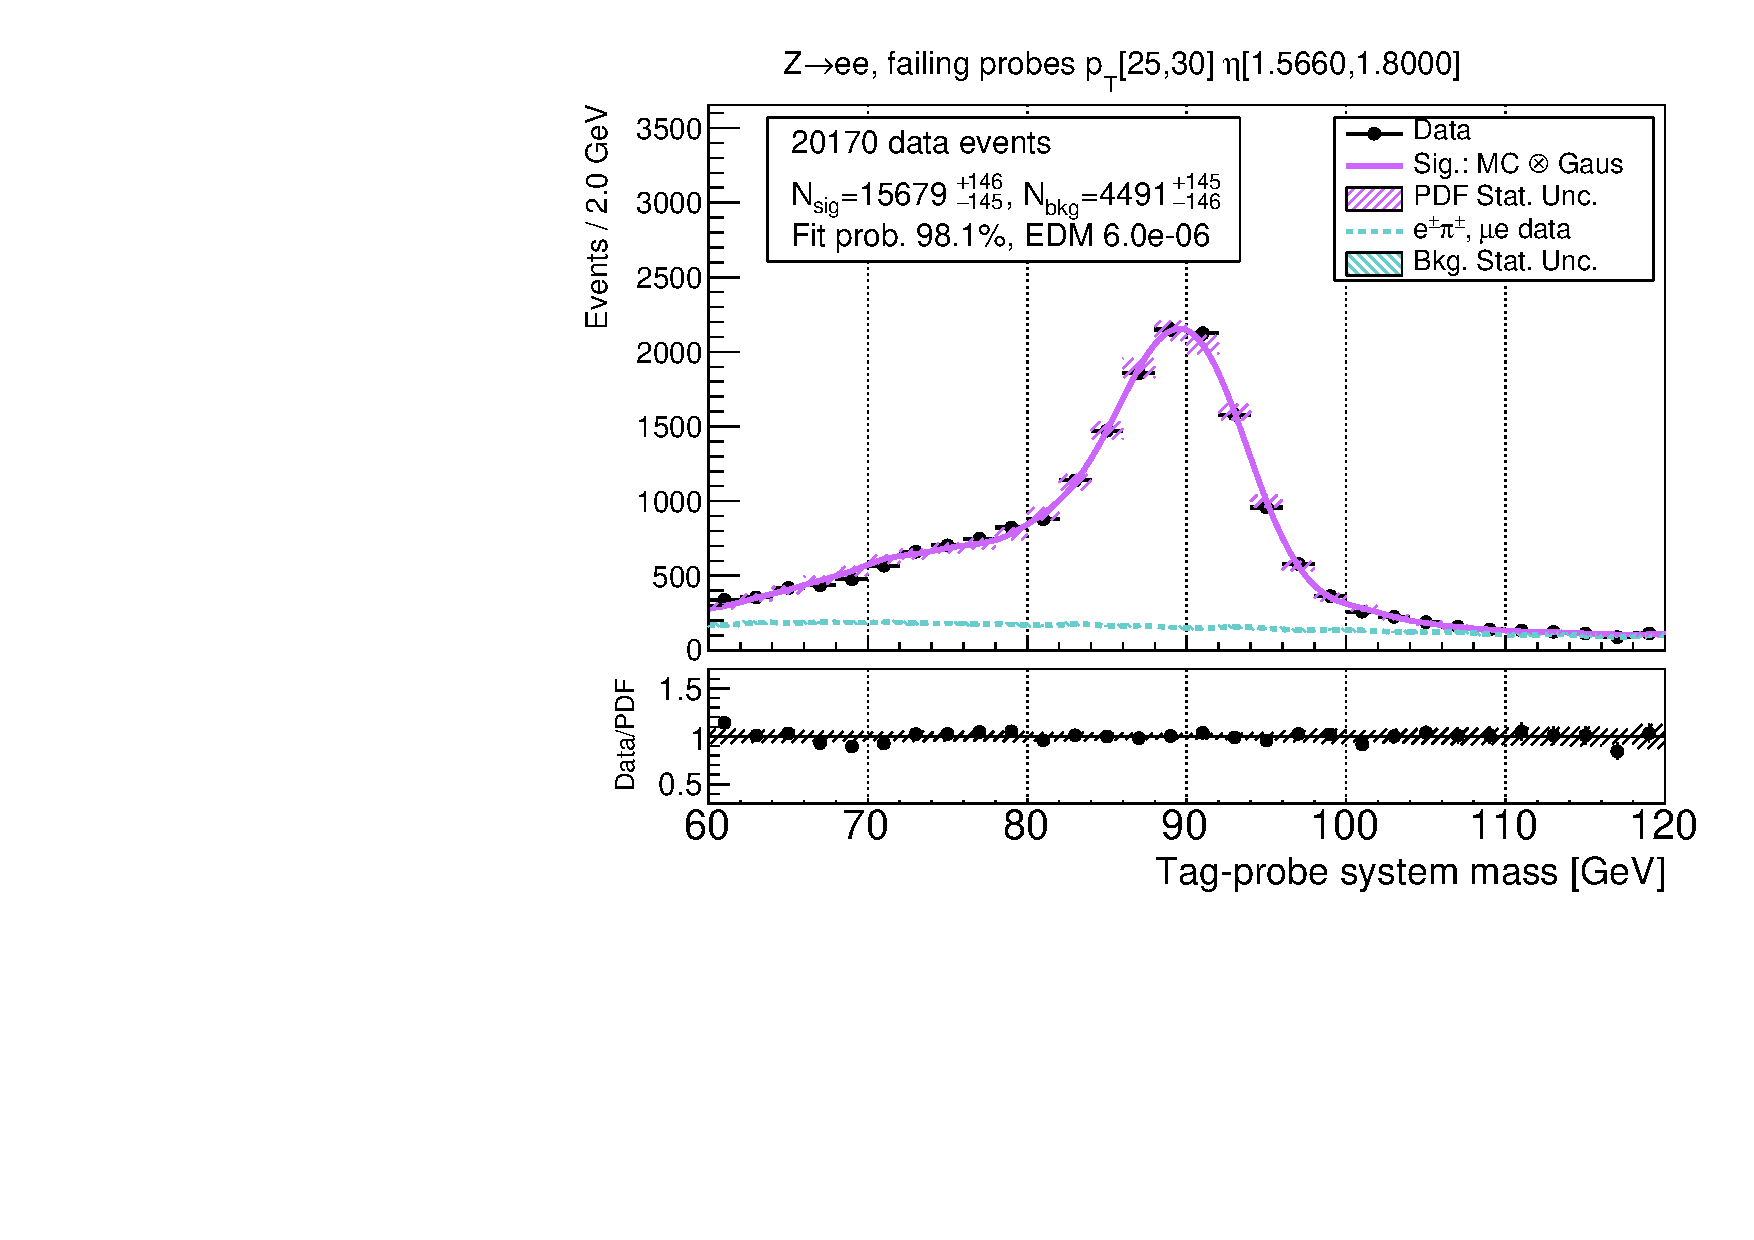
\includegraphics[width=0.49\textwidth]{figures/Zee_RecoTemplate_BkgLPiEMu_fail_ptBin3_etaBin23.pdf}
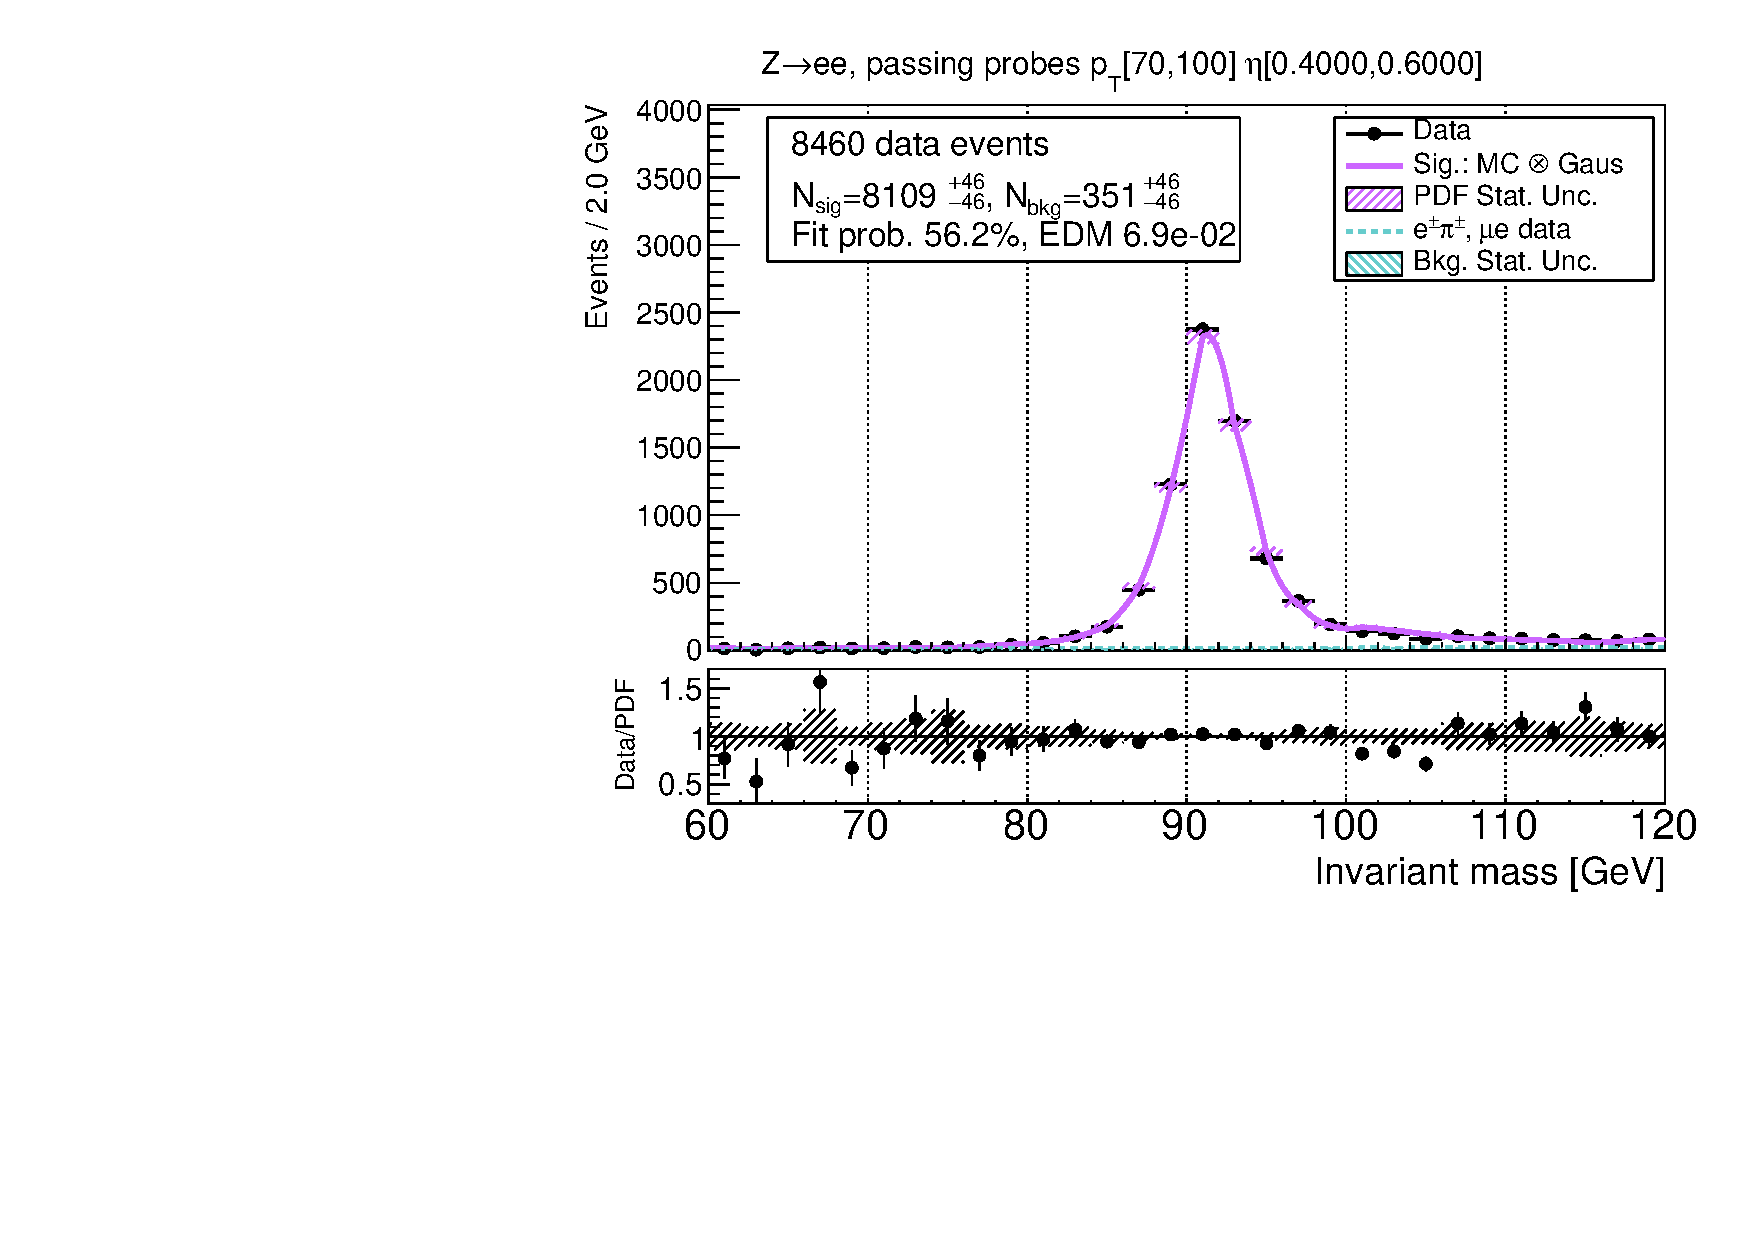
\includegraphics[width=0.49\textwidth]{figures/Zee_RecoTemplate_BkgLPiEMu_pass_ptBin14_etaBin17.pdf}
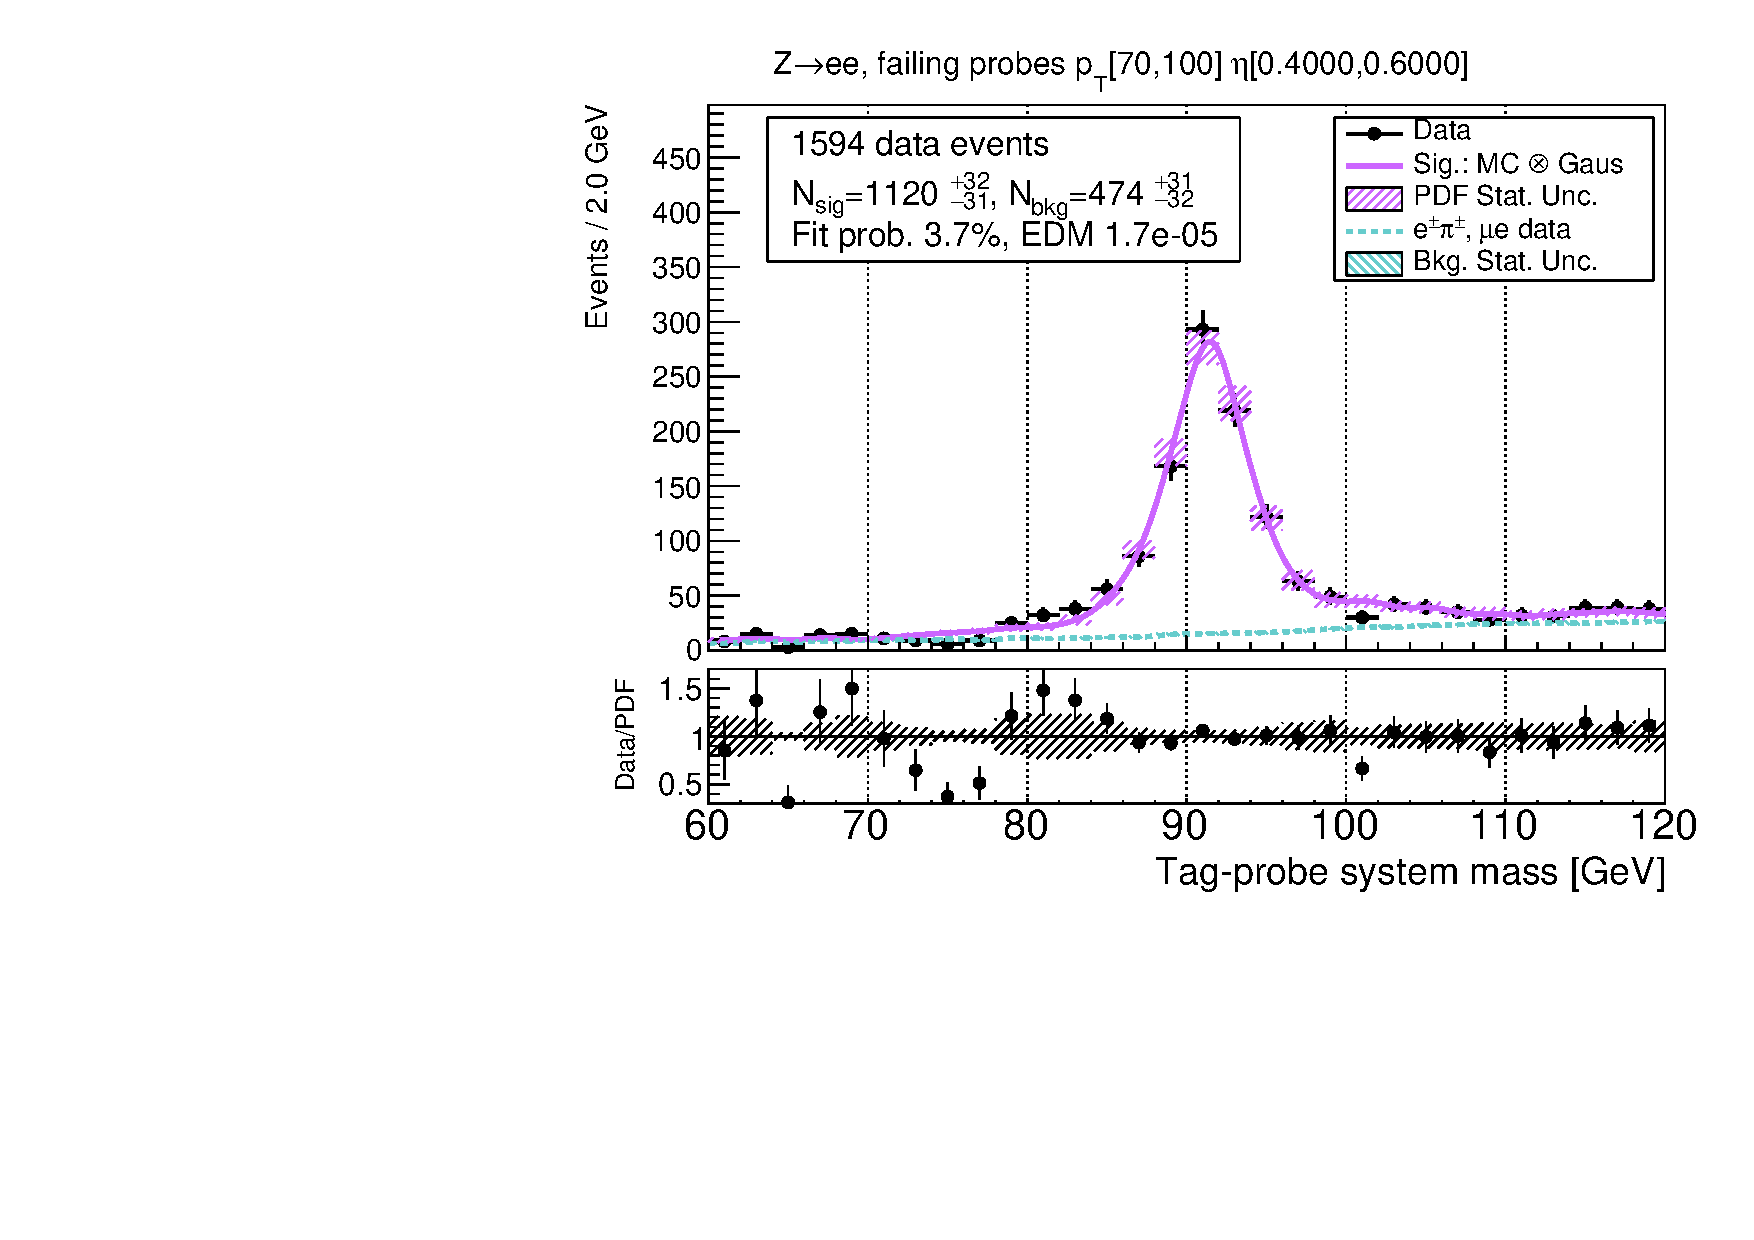
\includegraphics[width=0.49\textwidth]{figures/Zee_RecoTemplate_BkgLPiEMu_fail_ptBin14_etaBin17.pdf}
\caption{Efficiency extraction fits for the Medium electron working point using the data-driven background shape, at higher values of electron transverse momentum.}
\label{fig:ZeeNominalFits2}
\end{figure}

\section{Lepton efficiencies and scale factors}
\textcolor{red}{\bf{MOVE THIS TO APPENDICES?}}
\subsection{Medium muon efficiencies and scale factors}
The extracted data efficiencies are shown in Figure~\ref{fig:ZmmDataEff}.
The MC efficiencies from counting are shown in Figure~\ref{fig:ZmmMCEff}.
The Data/MC efficiency scale factors are shown in Figure~\ref{fig:ZmmScaleFactors}, with
propagated statistical errors in Figures~\ref{fig:ZmmScaleFactorsErrorHi} and~\ref{fig:ZmmScaleFactorsErrorLo}.
The main feature is a drop in the efficiency for low-energy muons in the central detector region.
\begin{figure}
\centering
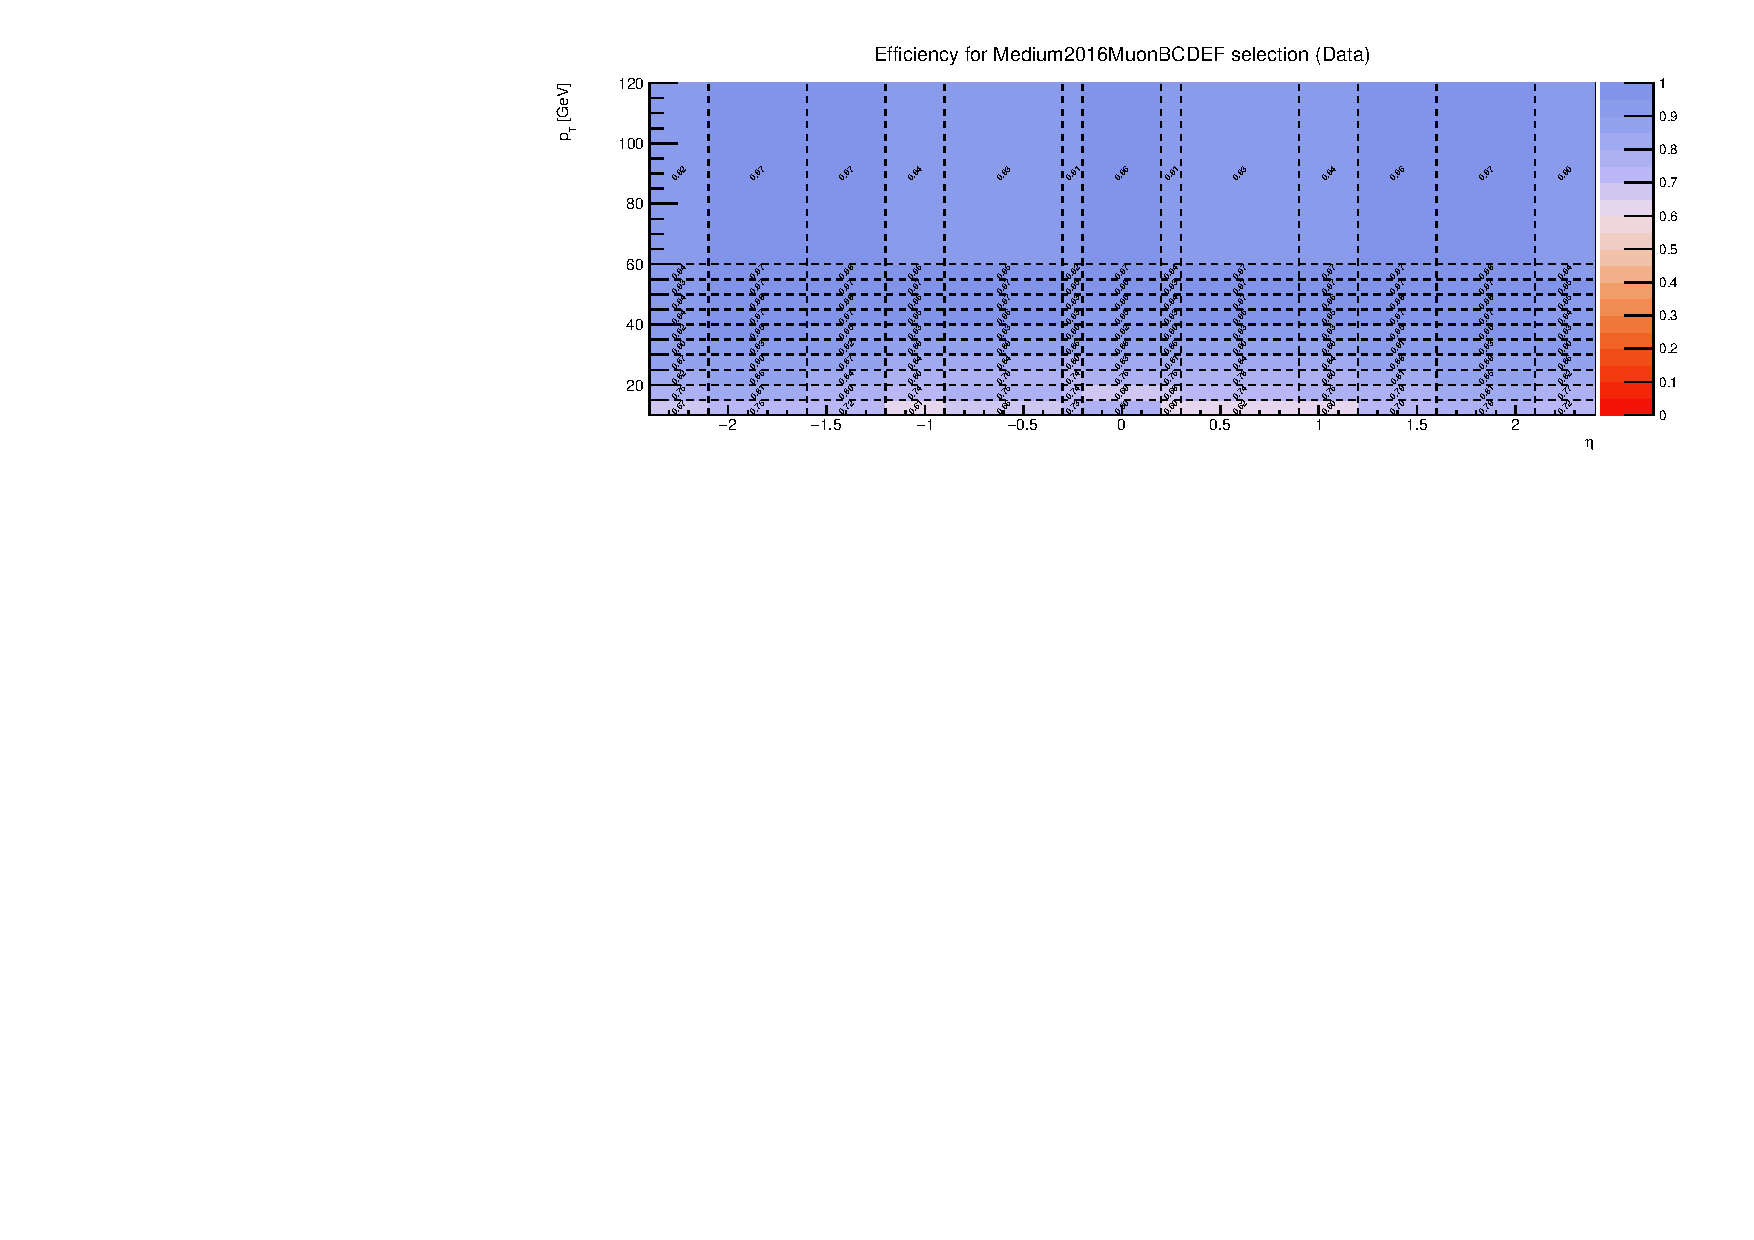
\includegraphics[width=1.00\textwidth]{{figures/eff_data_Medium2016MuonBCDEF_0.0-0.0_10.0-120.0}.pdf}
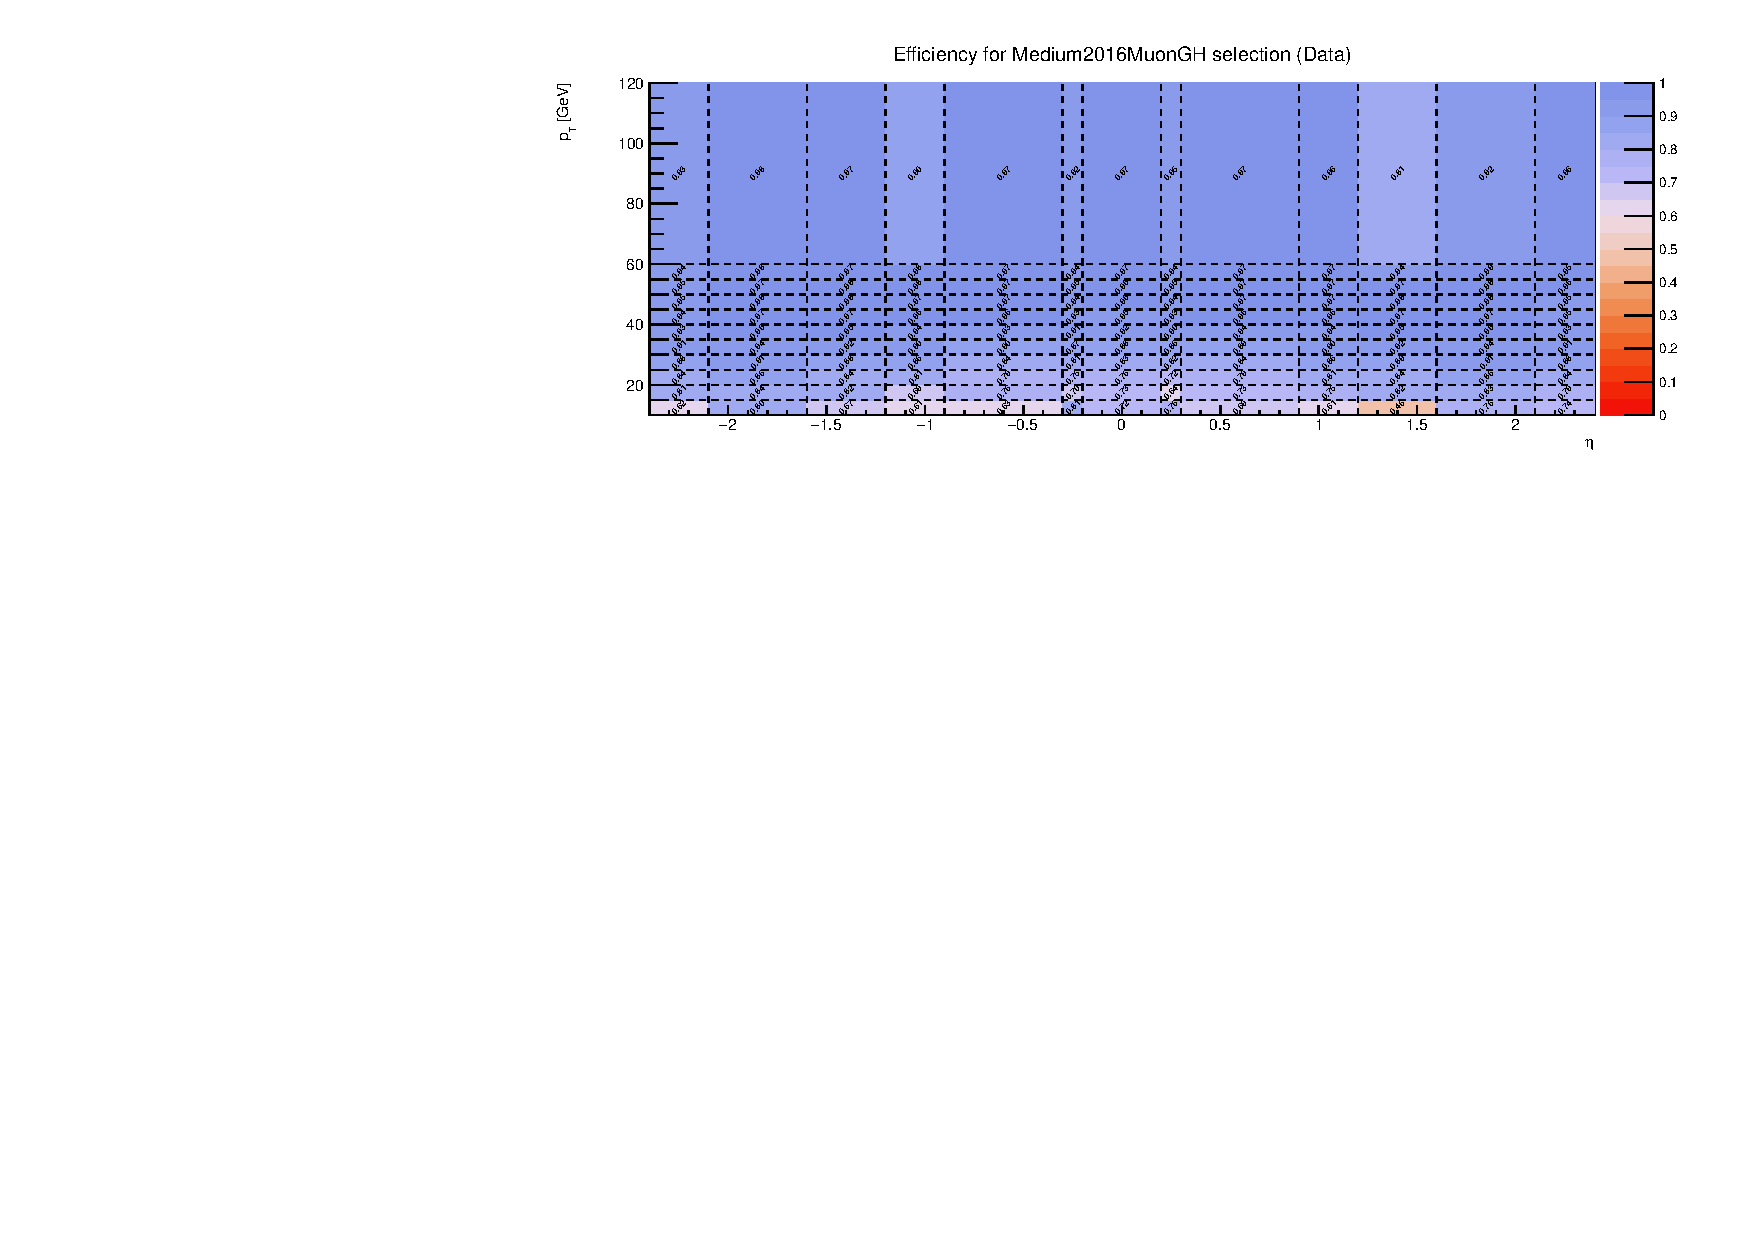
\includegraphics[width=1.00\textwidth]{{figures/eff_data_Medium2016MuonGH_0.0-0.0_10.0-120.0}.pdf}
\caption{Efficiencies extracted from data for the Medium muon working point in 2016 run eras B to F, and G to H.}
\label{fig:ZmmDataEff}
\end{figure}
\begin{figure}
\centering
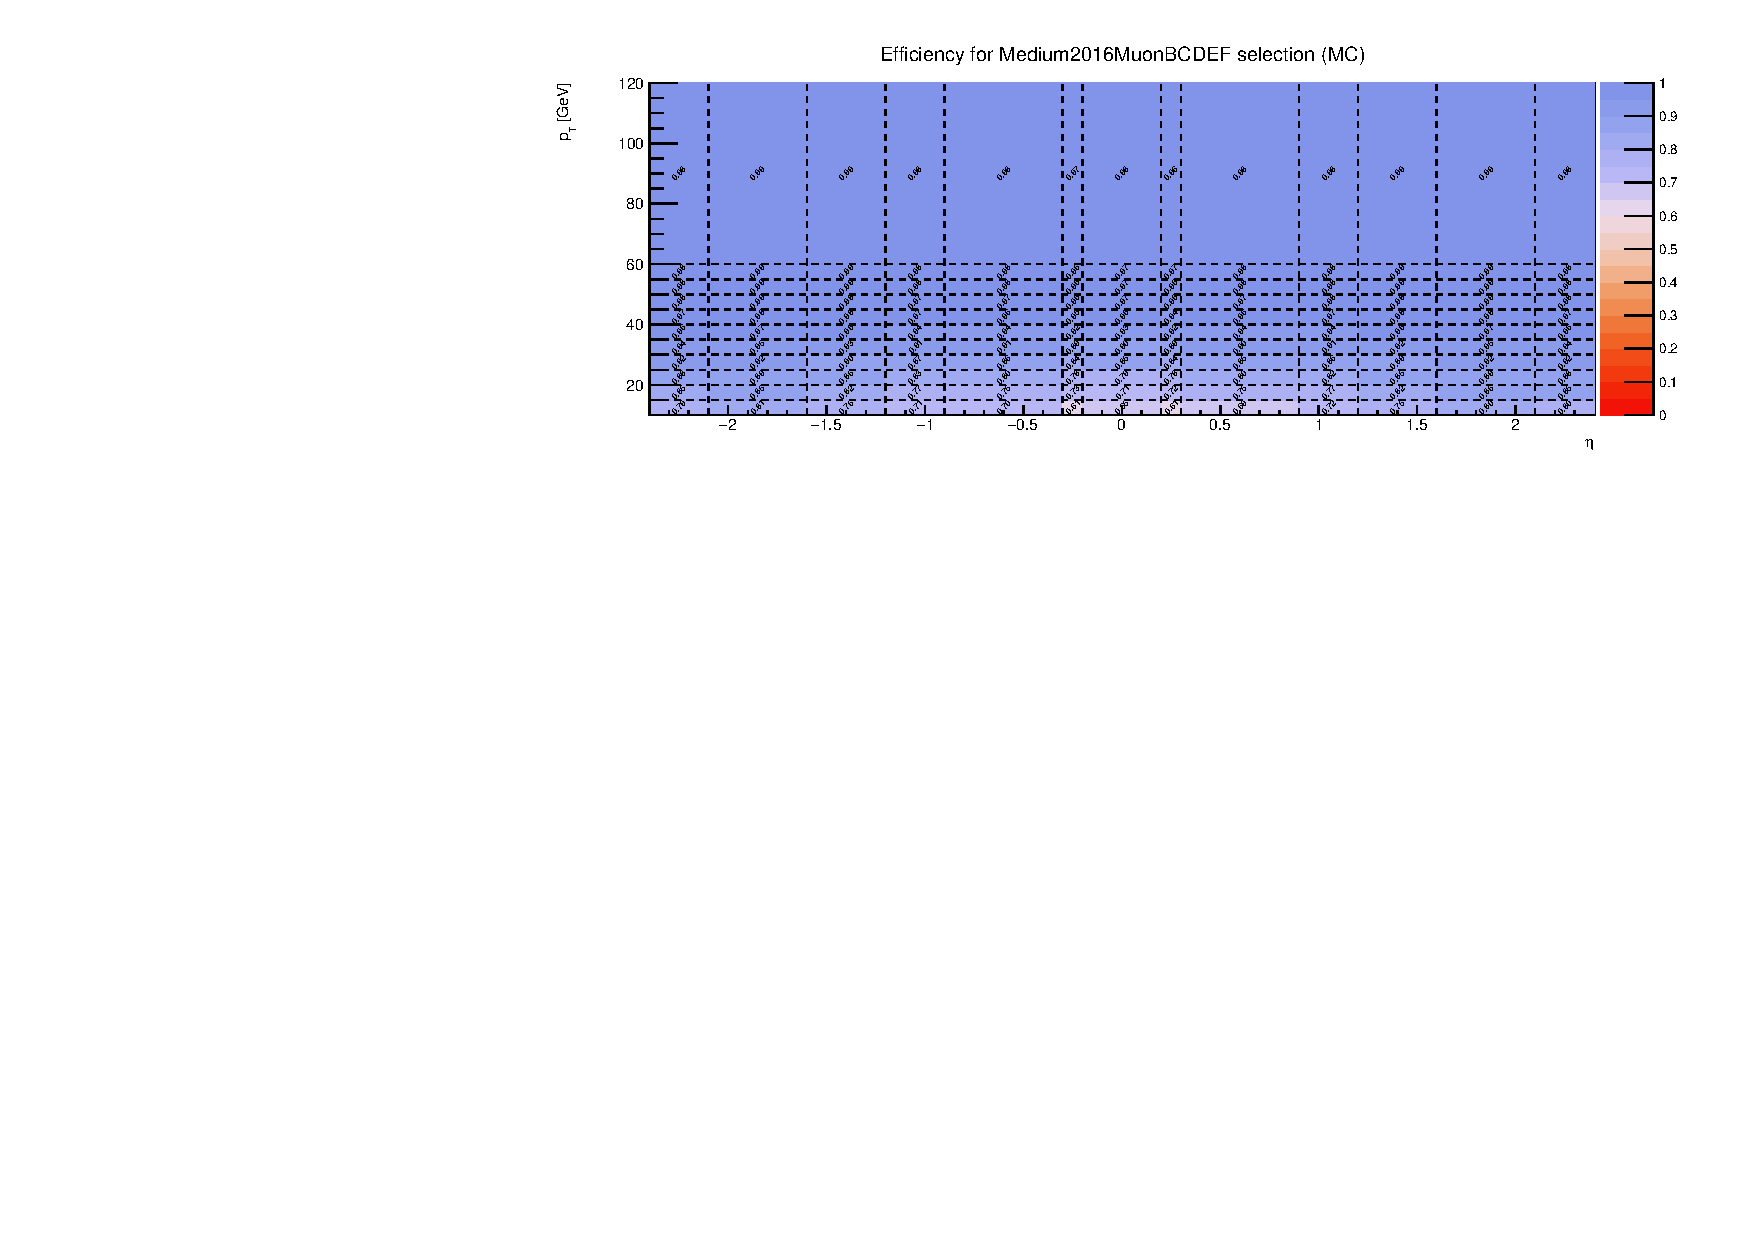
\includegraphics[width=1.00\textwidth]{{figures/eff_mc_Medium2016MuonBCDEF_0.0-0.0_10.0-120.0}.pdf}
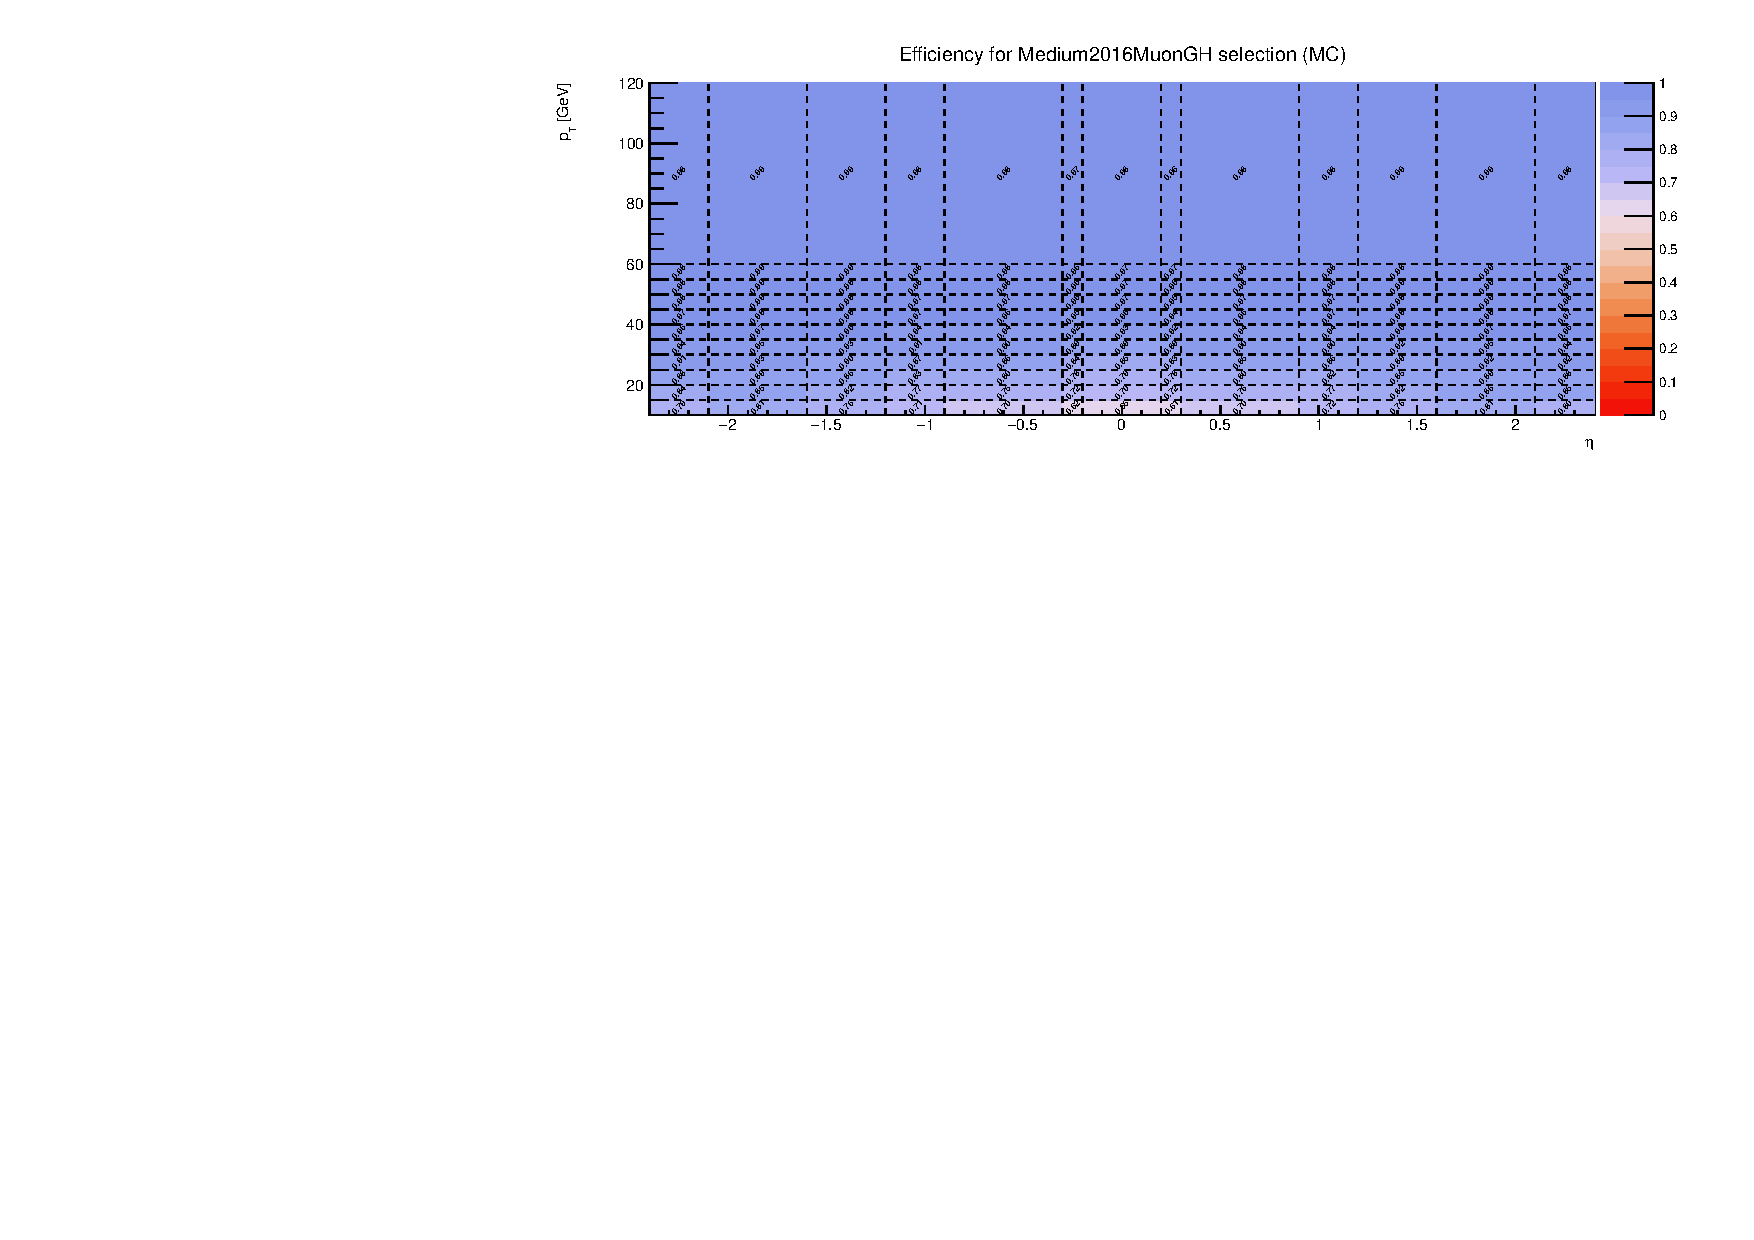
\includegraphics[width=1.00\textwidth]{{figures/eff_mc_Medium2016MuonGH_0.0-0.0_10.0-120.0}.pdf}
\caption{Efficiencies extracted from MC for the Medium muon working point after reweighting to the pileup profile in 2016 run eras B to F, and G to H.}
\label{fig:ZmmMCEff}
\end{figure}
\begin{figure}
\centering
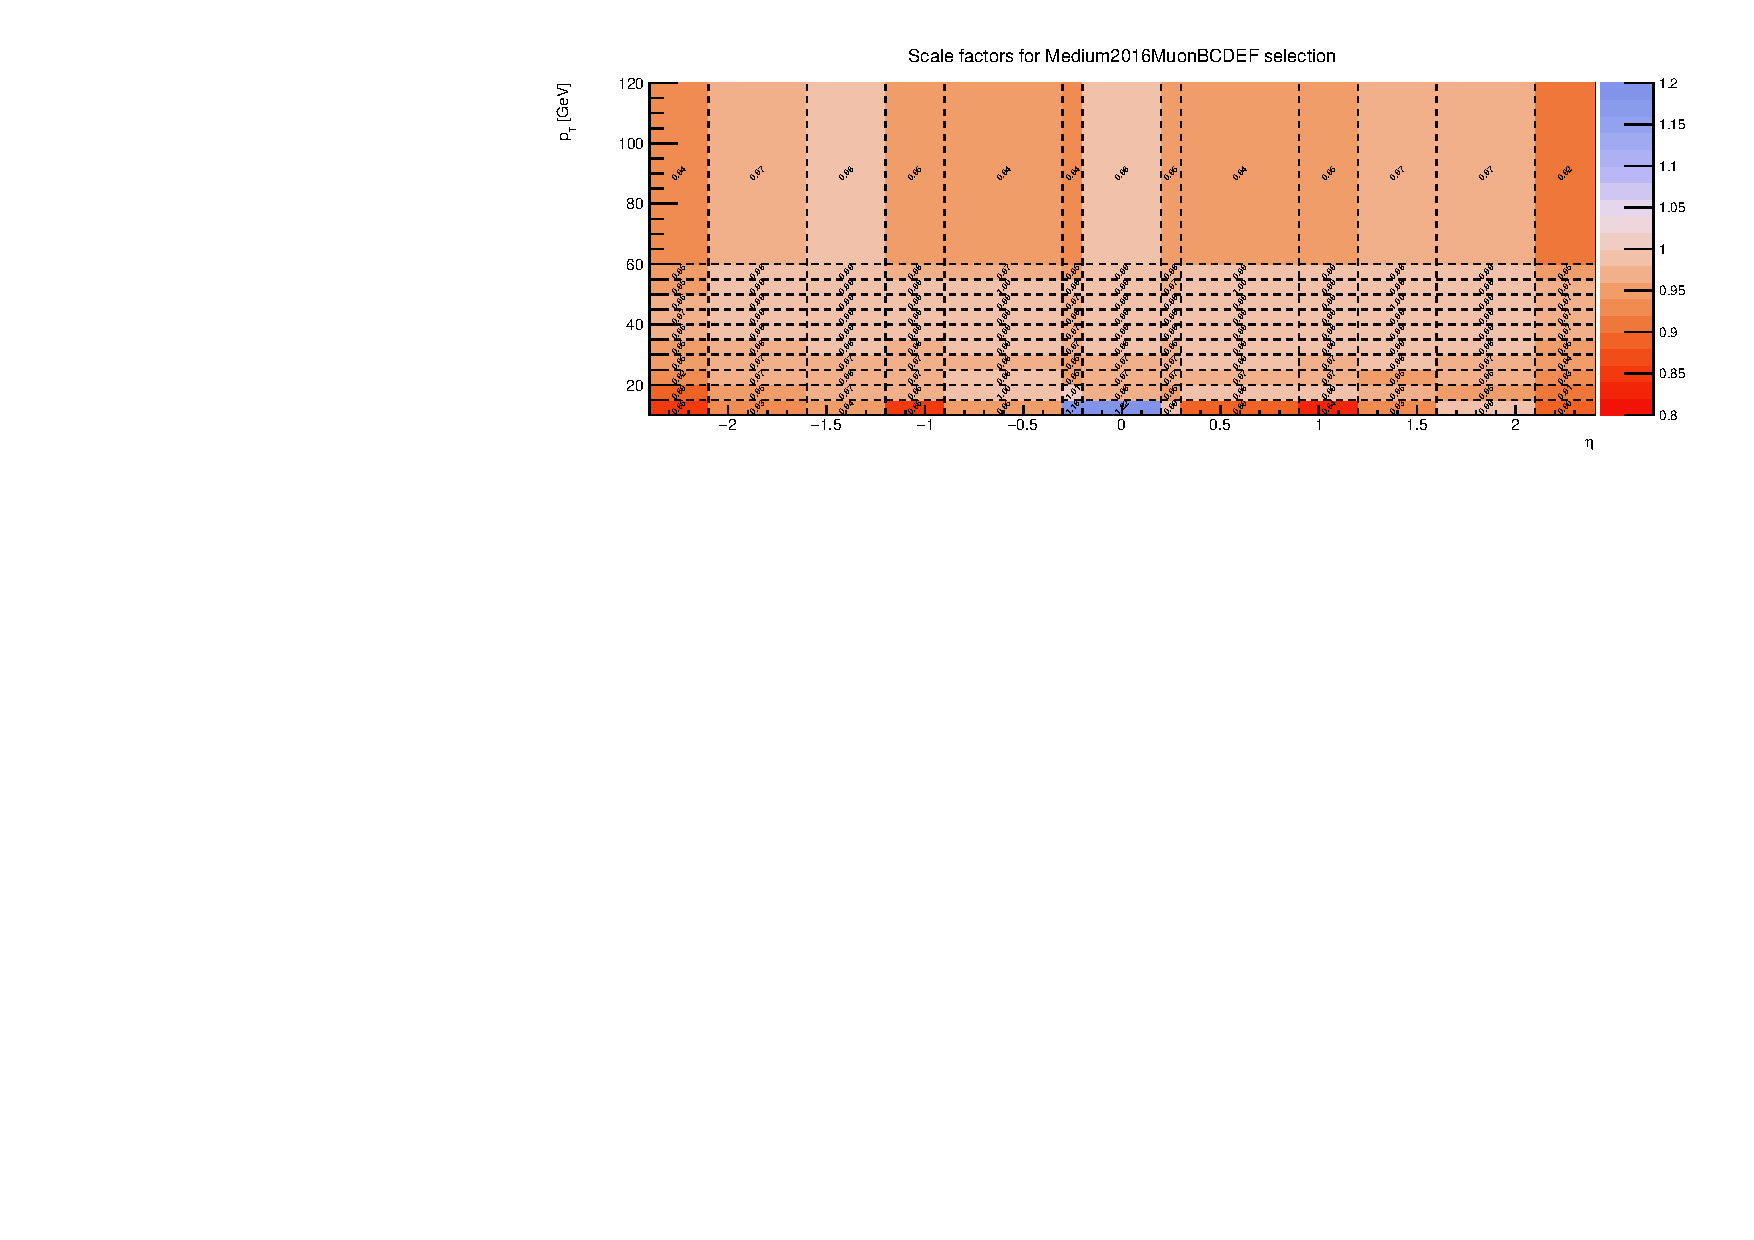
\includegraphics[width=1.00\textwidth]{{figures/scalefactors_Medium2016MuonBCDEF_0.0-0.0_10.0-120.0}.pdf}
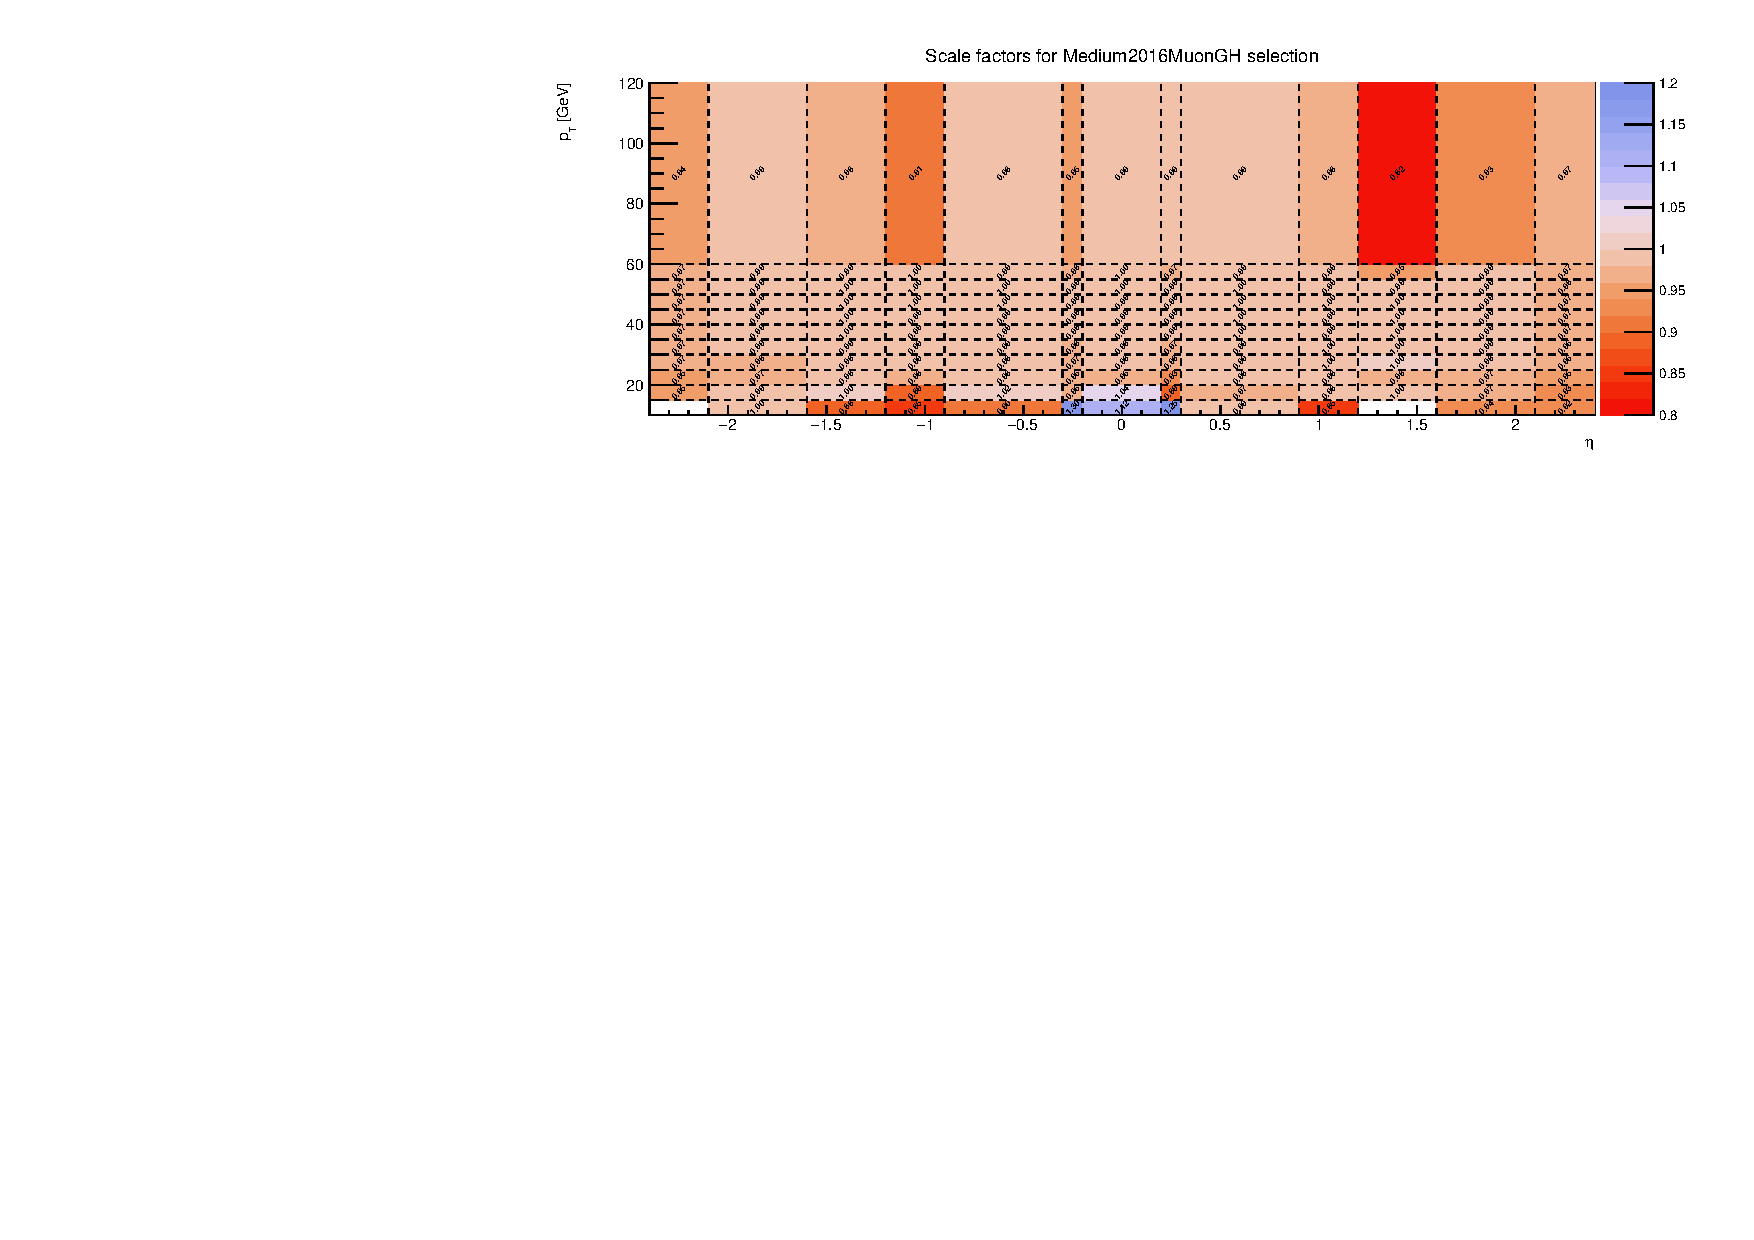
\includegraphics[width=1.00\textwidth]{{figures/scalefactors_Medium2016MuonGH_0.0-0.0_10.0-120.0}.pdf}
\caption{Scale factors derived from Data/MC efficiencies for the Medium muon working point in 2016 run eras B to F, and G to H.}
\label{fig:ZmmScaleFactors}
\end{figure}
\begin{figure}
\centering
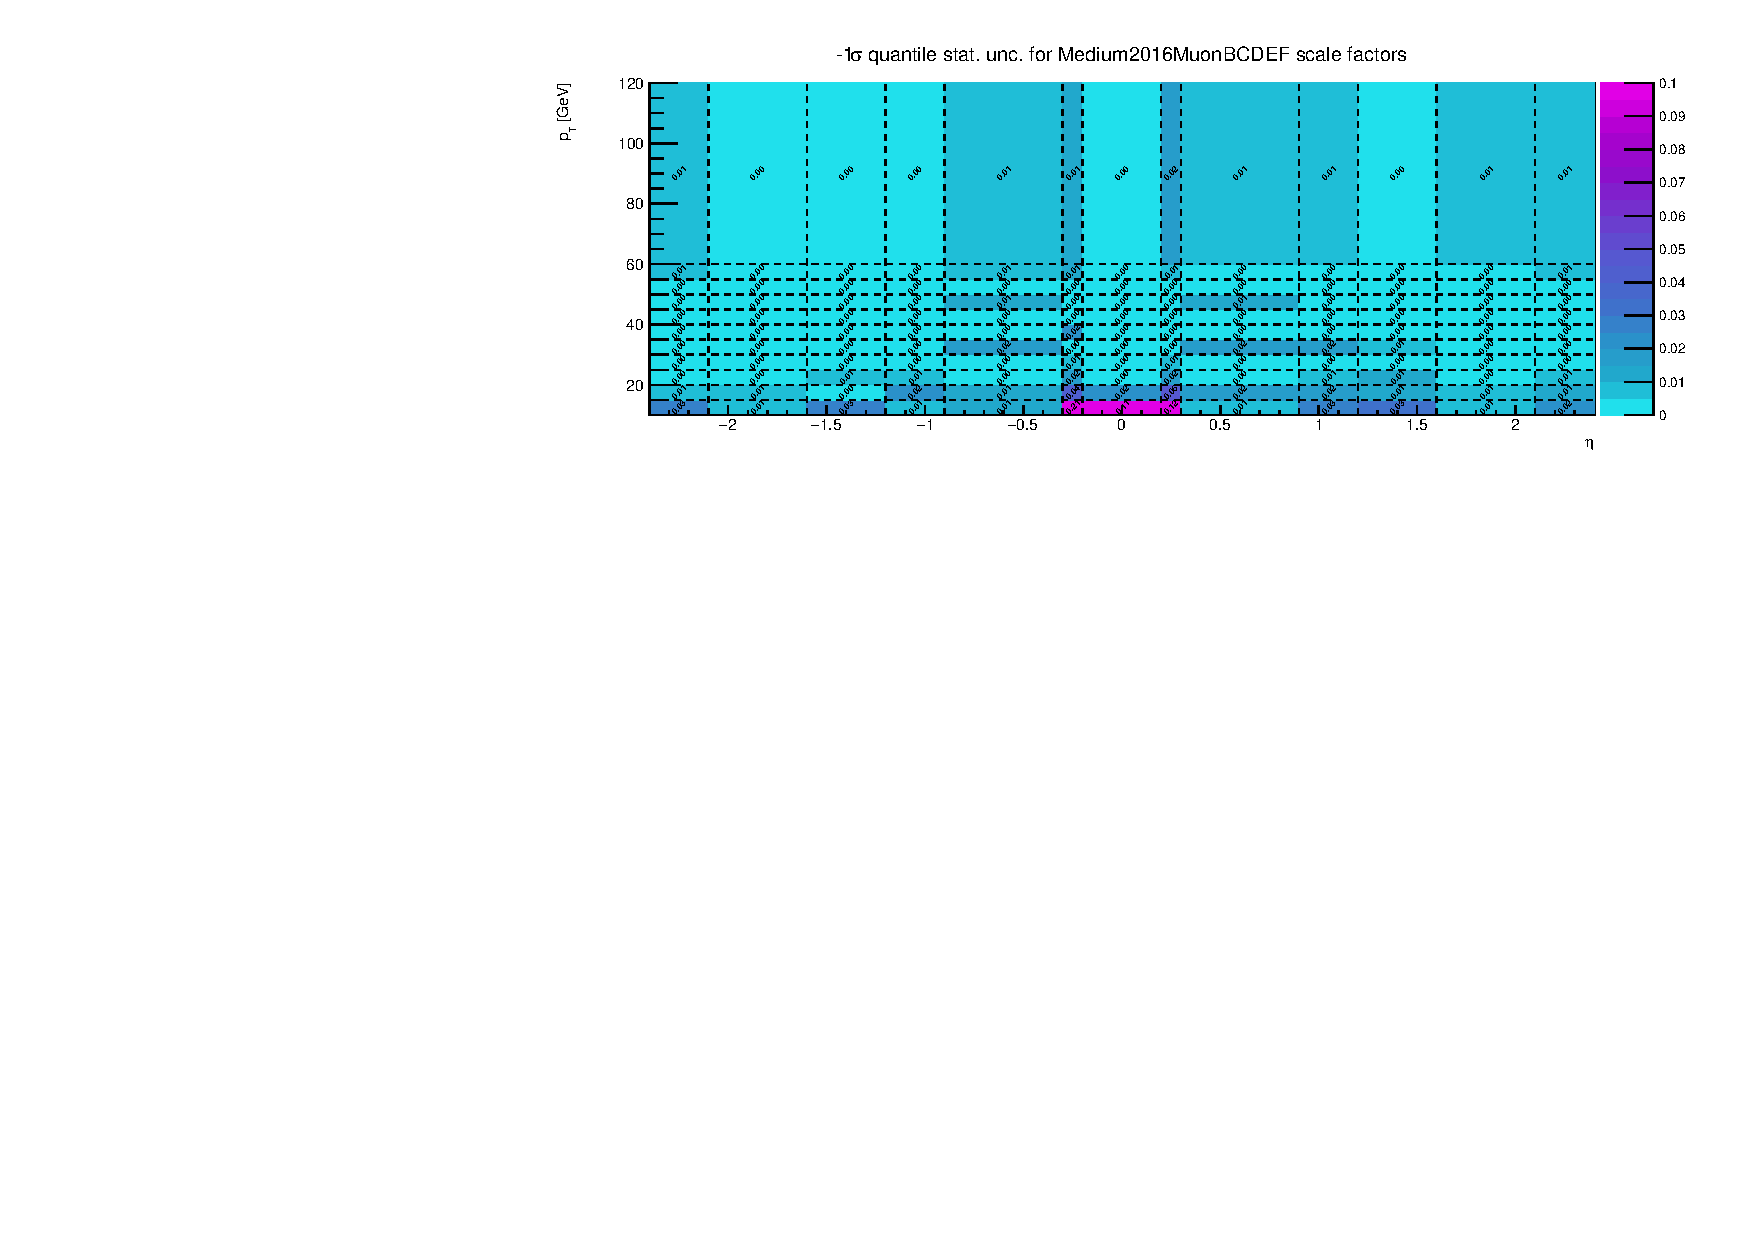
\includegraphics[width=1.00\textwidth]{{figures/scalefactors_Medium2016MuonBCDEF_statErrorLow_0.0-0.0_10.0-120.0}.pdf}
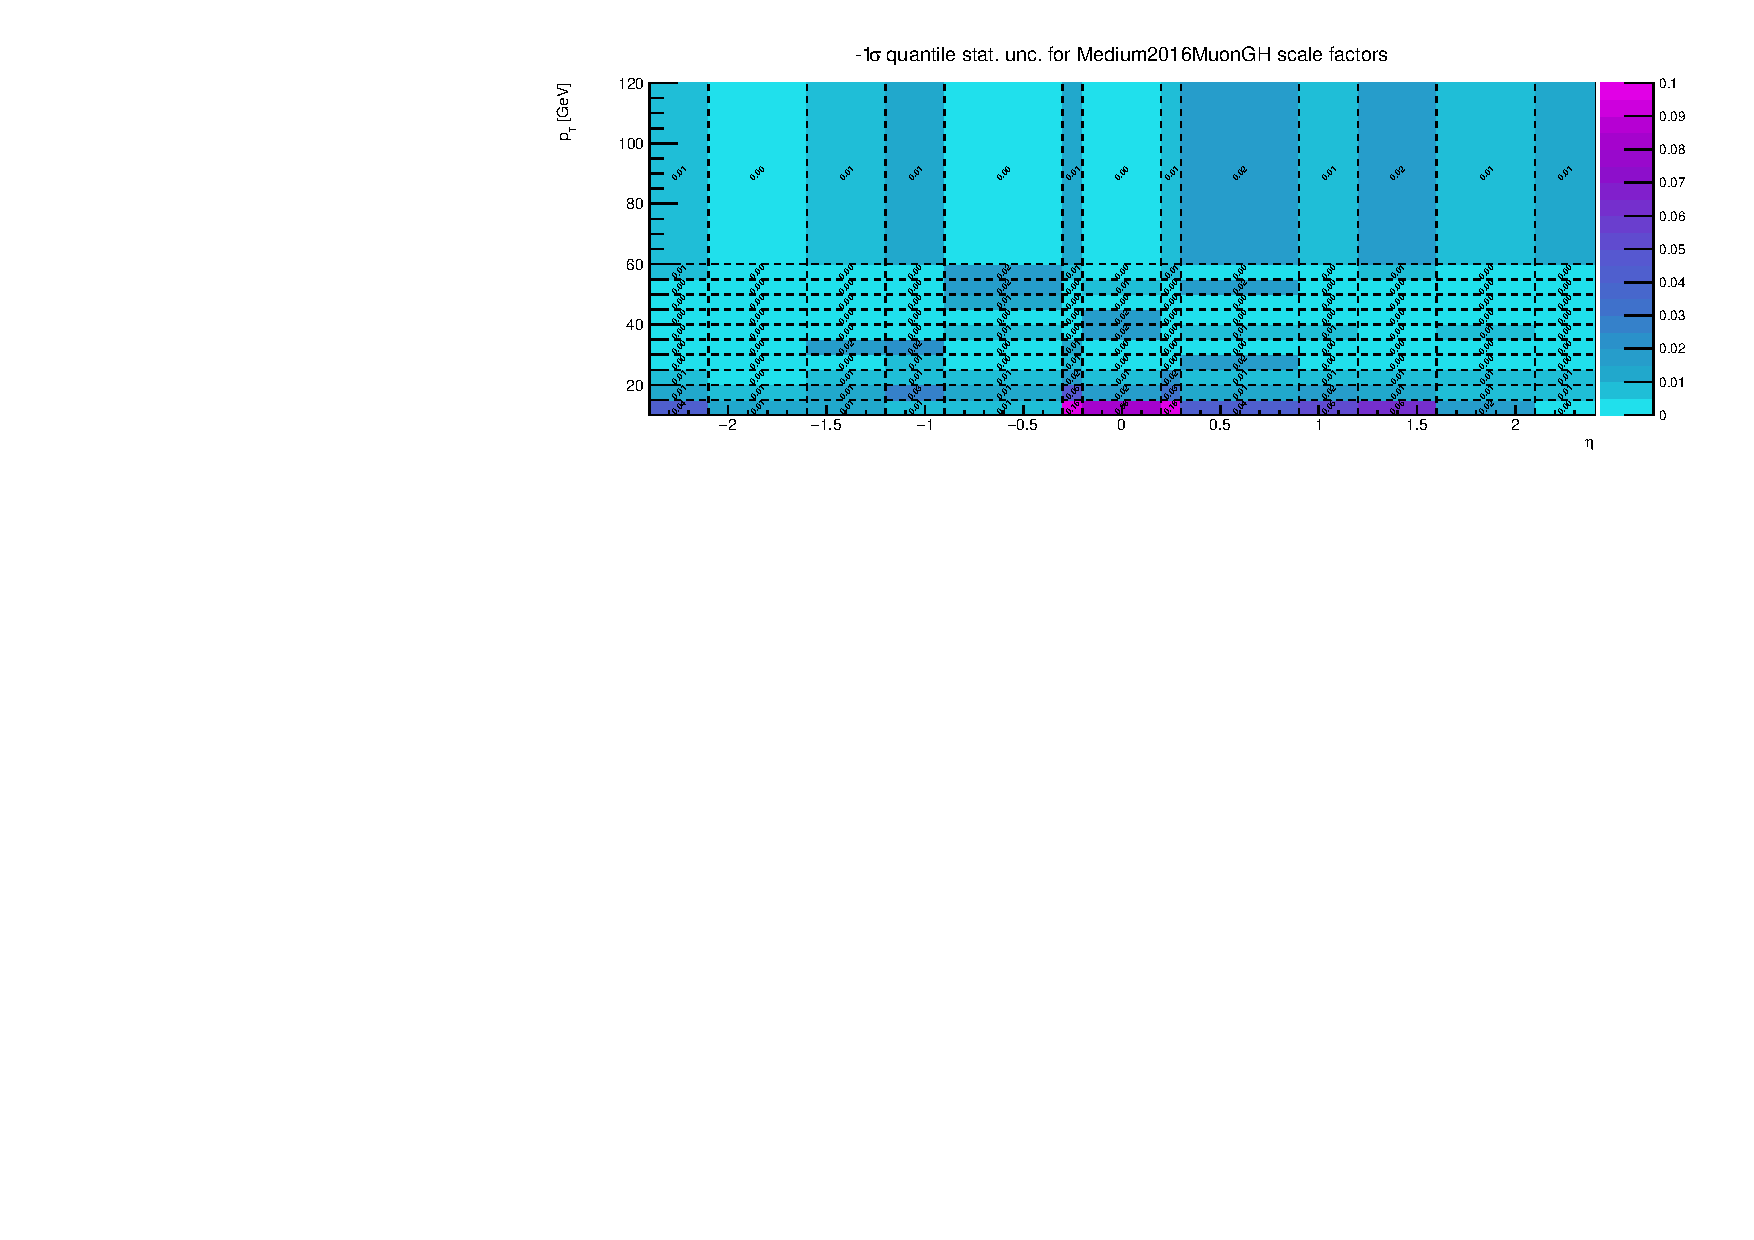
\includegraphics[width=1.00\textwidth]{{figures/scalefactors_Medium2016MuonGH_statErrorLow_0.0-0.0_10.0-120.0}.pdf}
\caption{Statistical uncertainties on the Medium muon scale factors (negative error) in 2016 run eras B to F, and G to H.}
\label{fig:ZmmScaleFactorsErrorHi}
\end{figure}
\begin{figure}
\centering
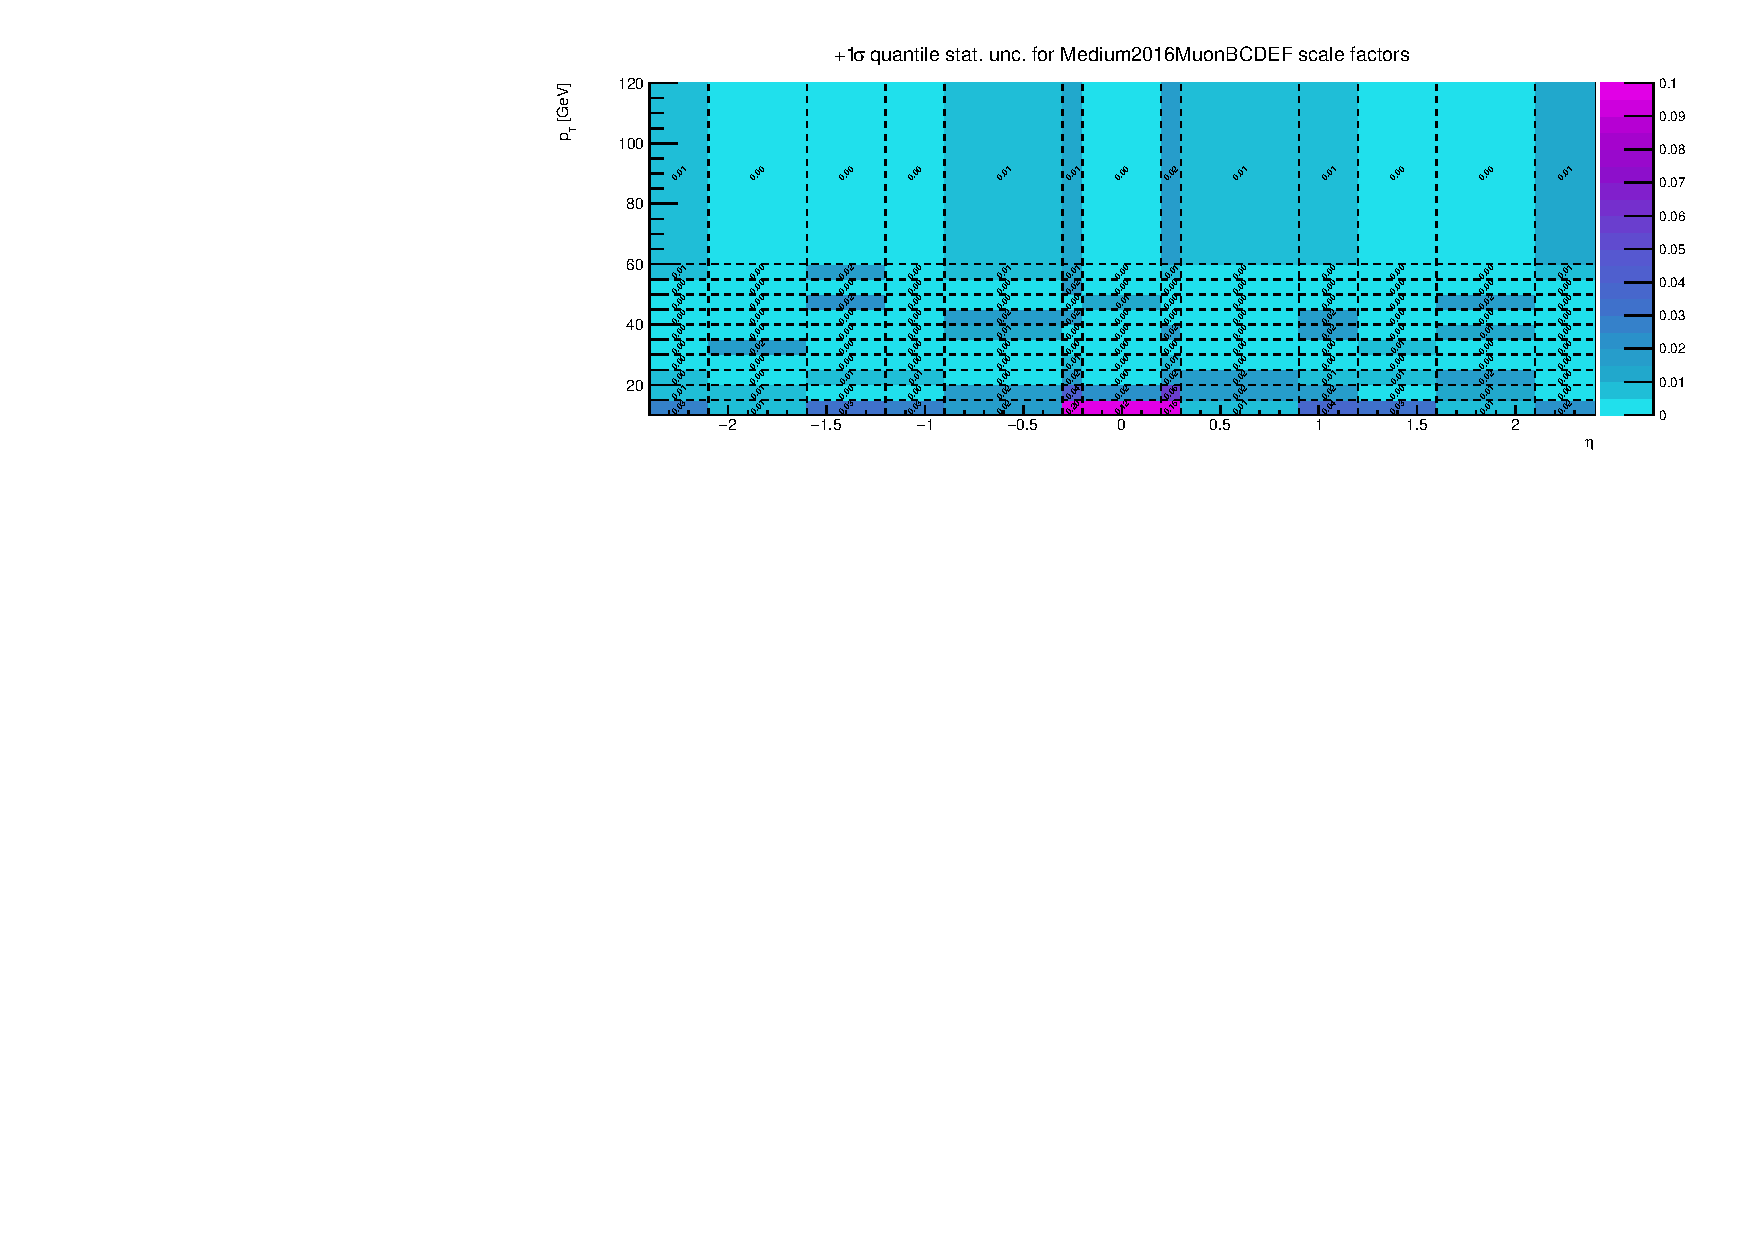
\includegraphics[width=1.00\textwidth]{{figures/scalefactors_Medium2016MuonBCDEF_statErrorHigh_0.0-0.0_10.0-120.0}.pdf}
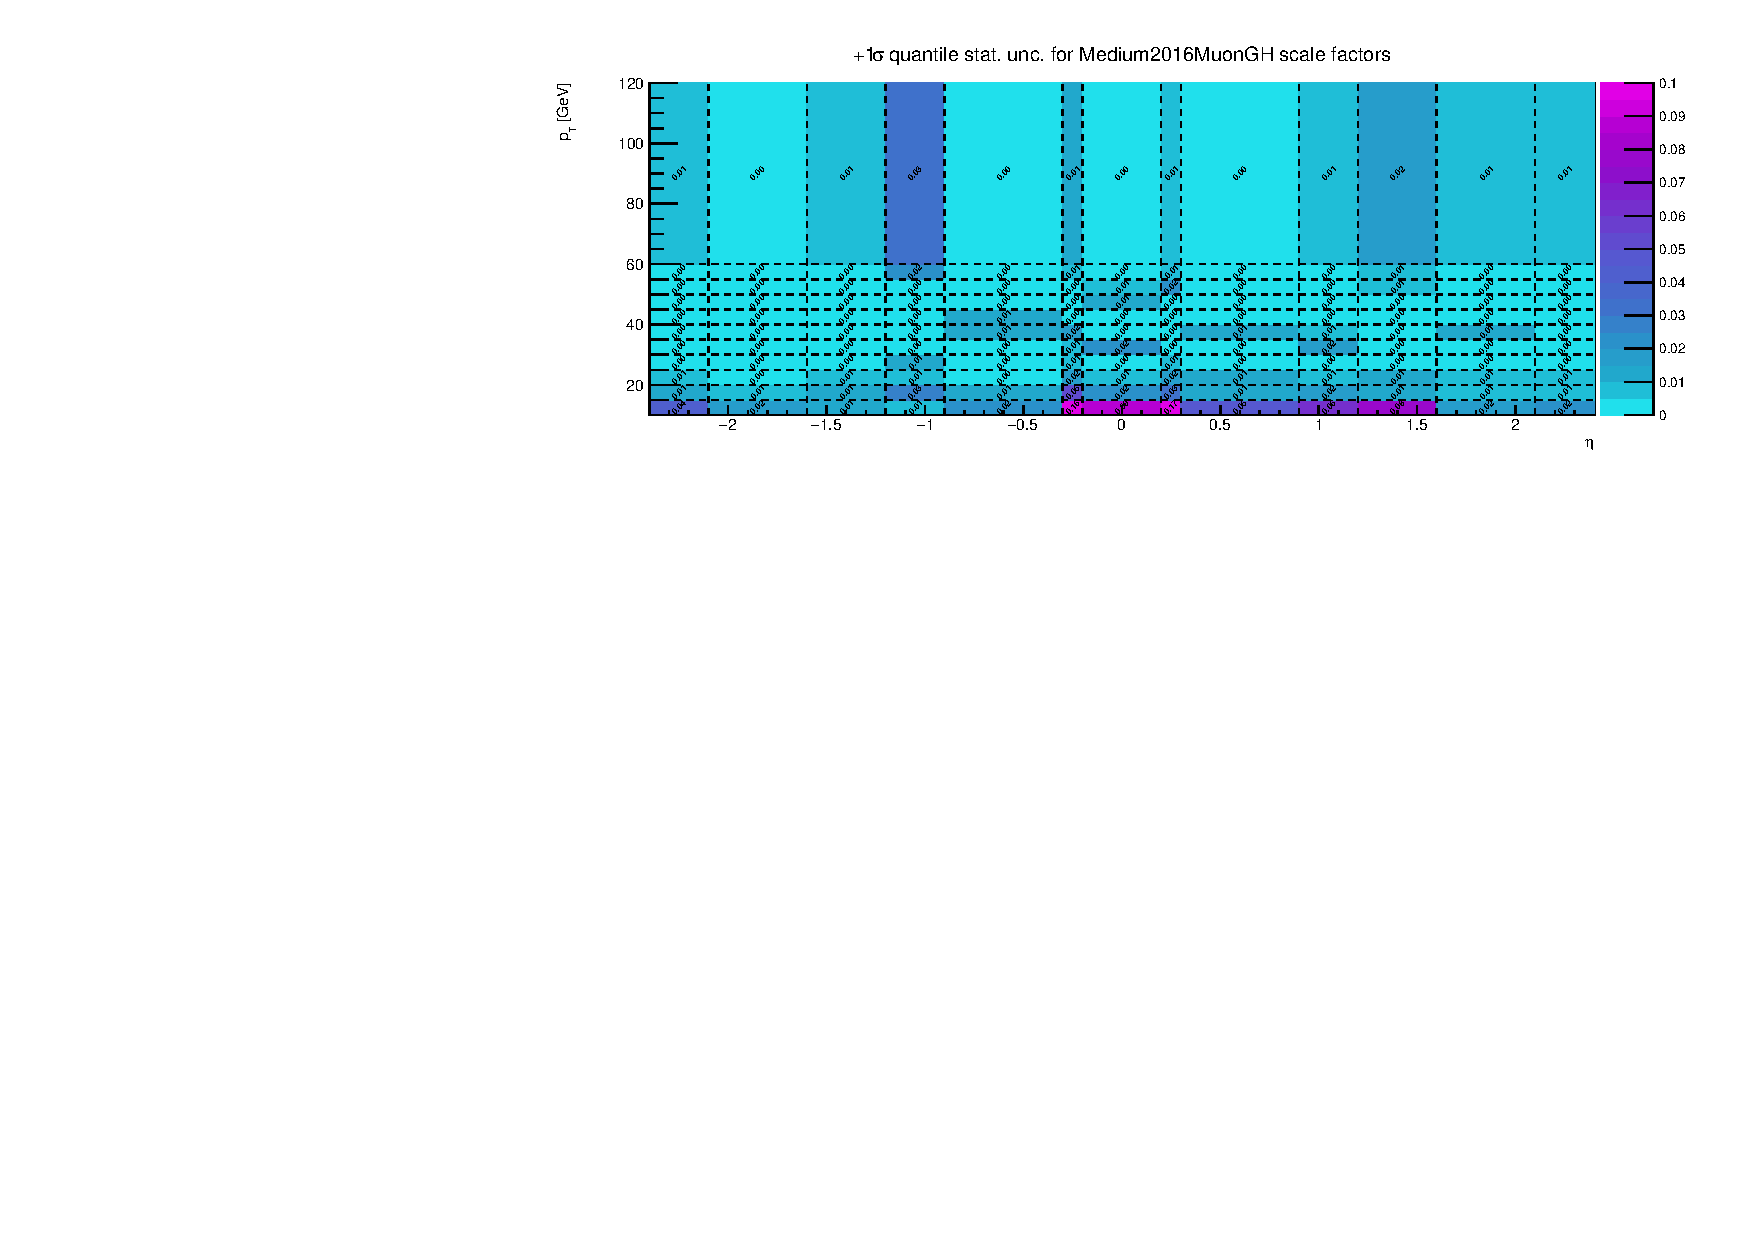
\includegraphics[width=1.00\textwidth]{{figures/scalefactors_Medium2016MuonGH_statErrorHigh_0.0-0.0_10.0-120.0}.pdf}
\caption{Statistical uncertainties on the Medium muon scale factors (positive error) in 2016 run eras B to F, and G to H.}
\label{fig:ZmmScaleFactorsErrorLo}
\end{figure}

\clearpage
\subsection{Medium electron efficiencies and scale factors}
The extracted data efficiencies are shown in Figure~\ref{fig:ZeeDataEff}.
The MC efficiencies from counting are shown in Figure~\ref{fig:ZeeMCEff}.
The Data/MC efficiency scale factors are shown in Figure~\ref{fig:ZeeScaleFactors}, with
propagated statistical errors in Figures~\ref{fig:ZeeScaleFactorsErrorHi} and~\ref{fig:ZeeScaleFactorsErrorLo}.
In general, the efficiencies are lower at lower energies or in the detector endcap ($\abs{\eta}>1.566$).
The scale factors reflect significant asymmetry in positive and negative values of $\eta$ and have a 
nonlinear structure in the endcap.

\begin{figure}
\centering
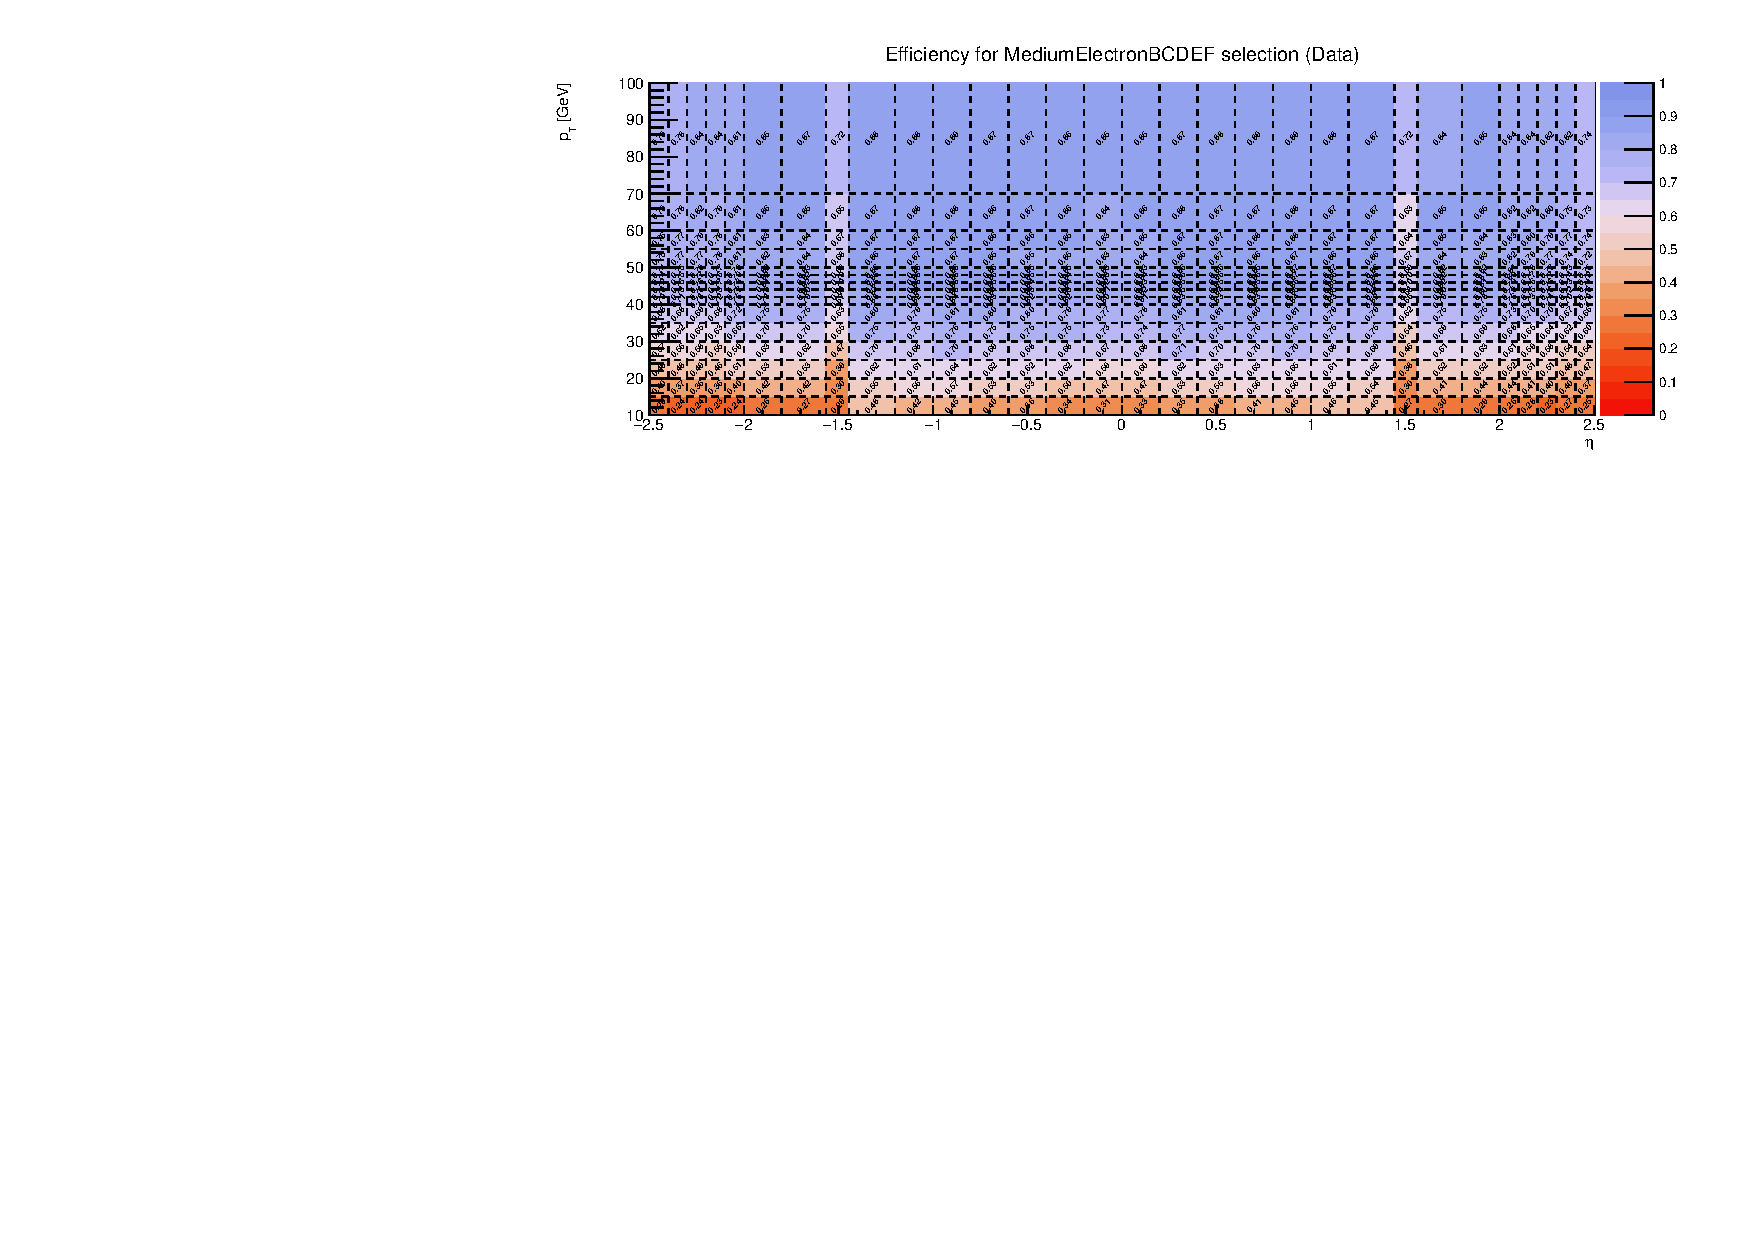
\includegraphics[width=1.00\textwidth]{{figures/eff_data_MediumElectronBCDEF_0.0-0.0_10.0-100.0}.pdf}
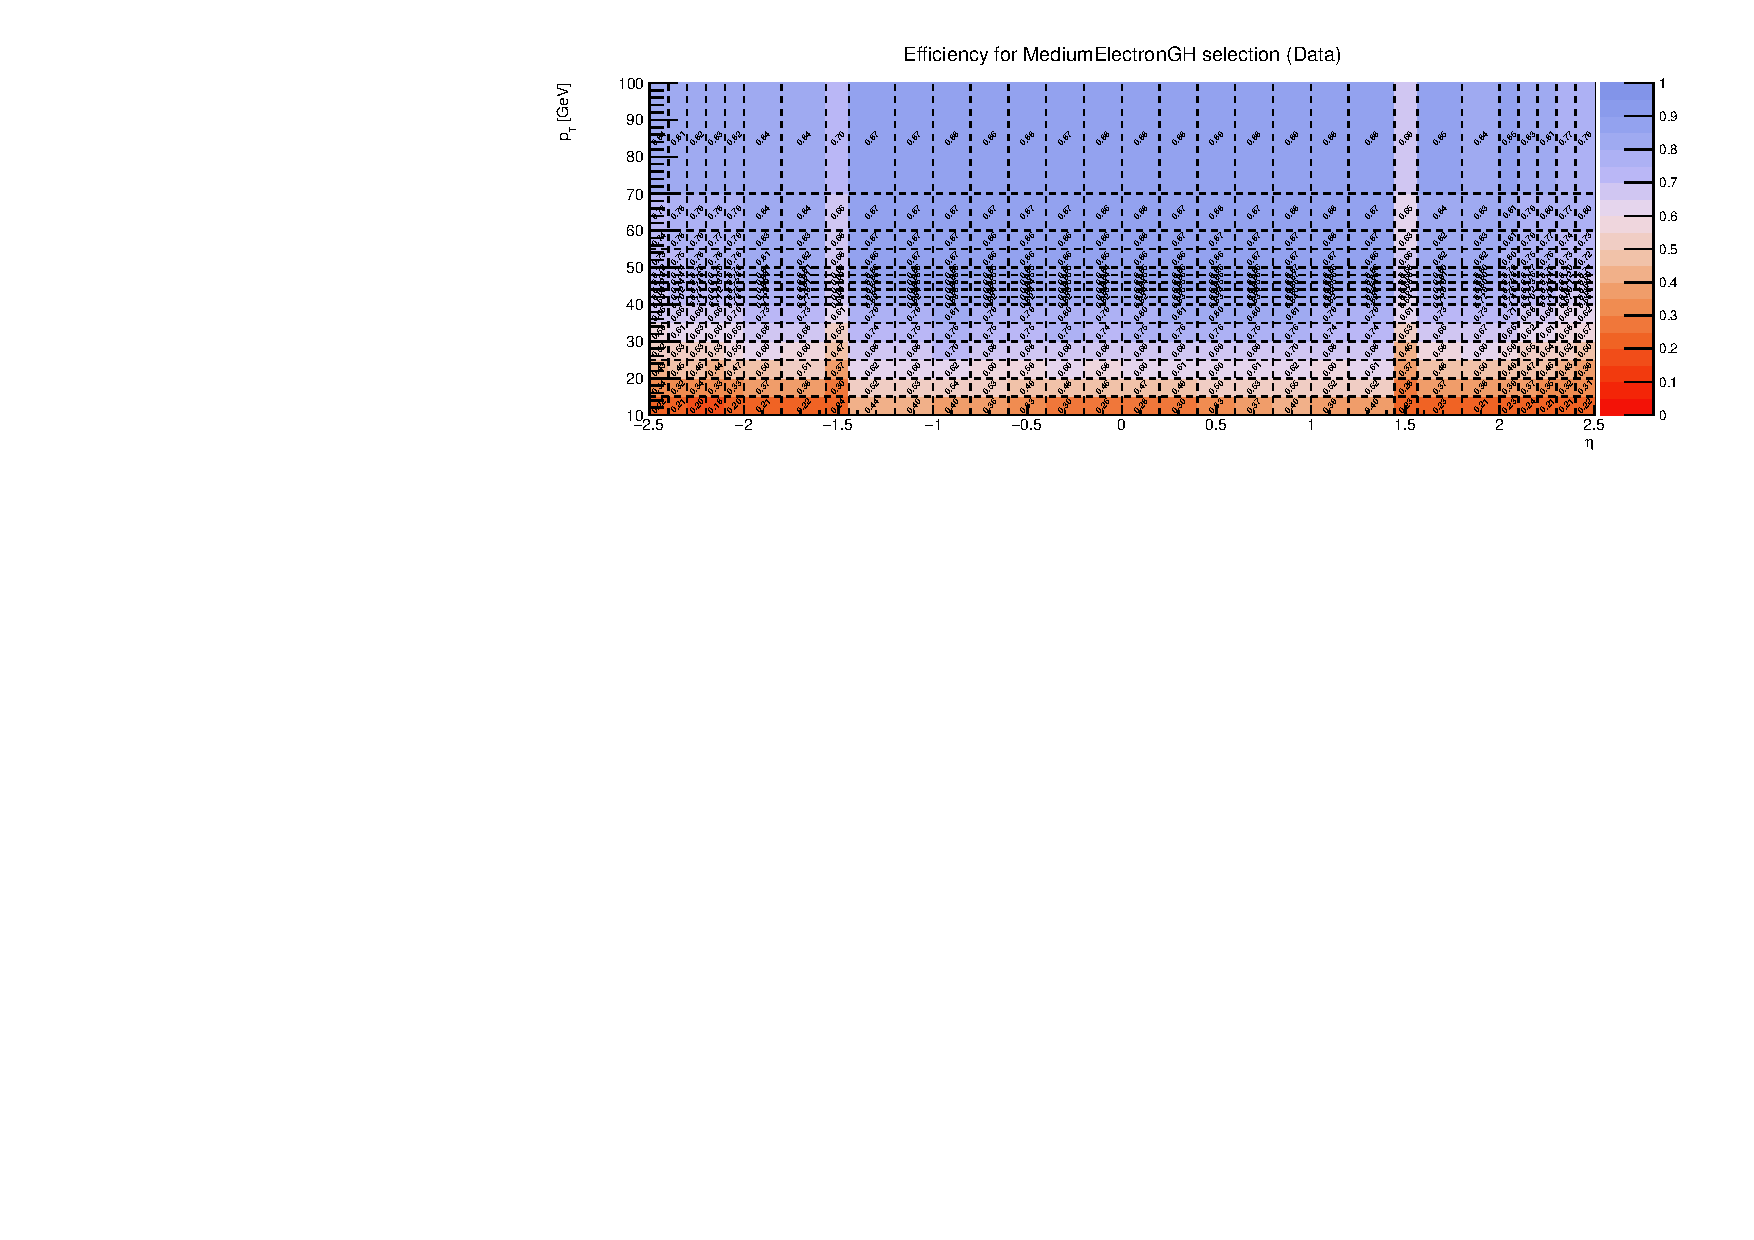
\includegraphics[width=1.00\textwidth]{{figures/eff_data_MediumElectronGH_0.0-0.0_10.0-100.0}.pdf}
\caption{Efficiencies extracted from data for the Medium electron working point in 2016 run eras B to F, and G to H.}
\label{fig:ZeeDataEff}
\end{figure}
\begin{figure}
\centering
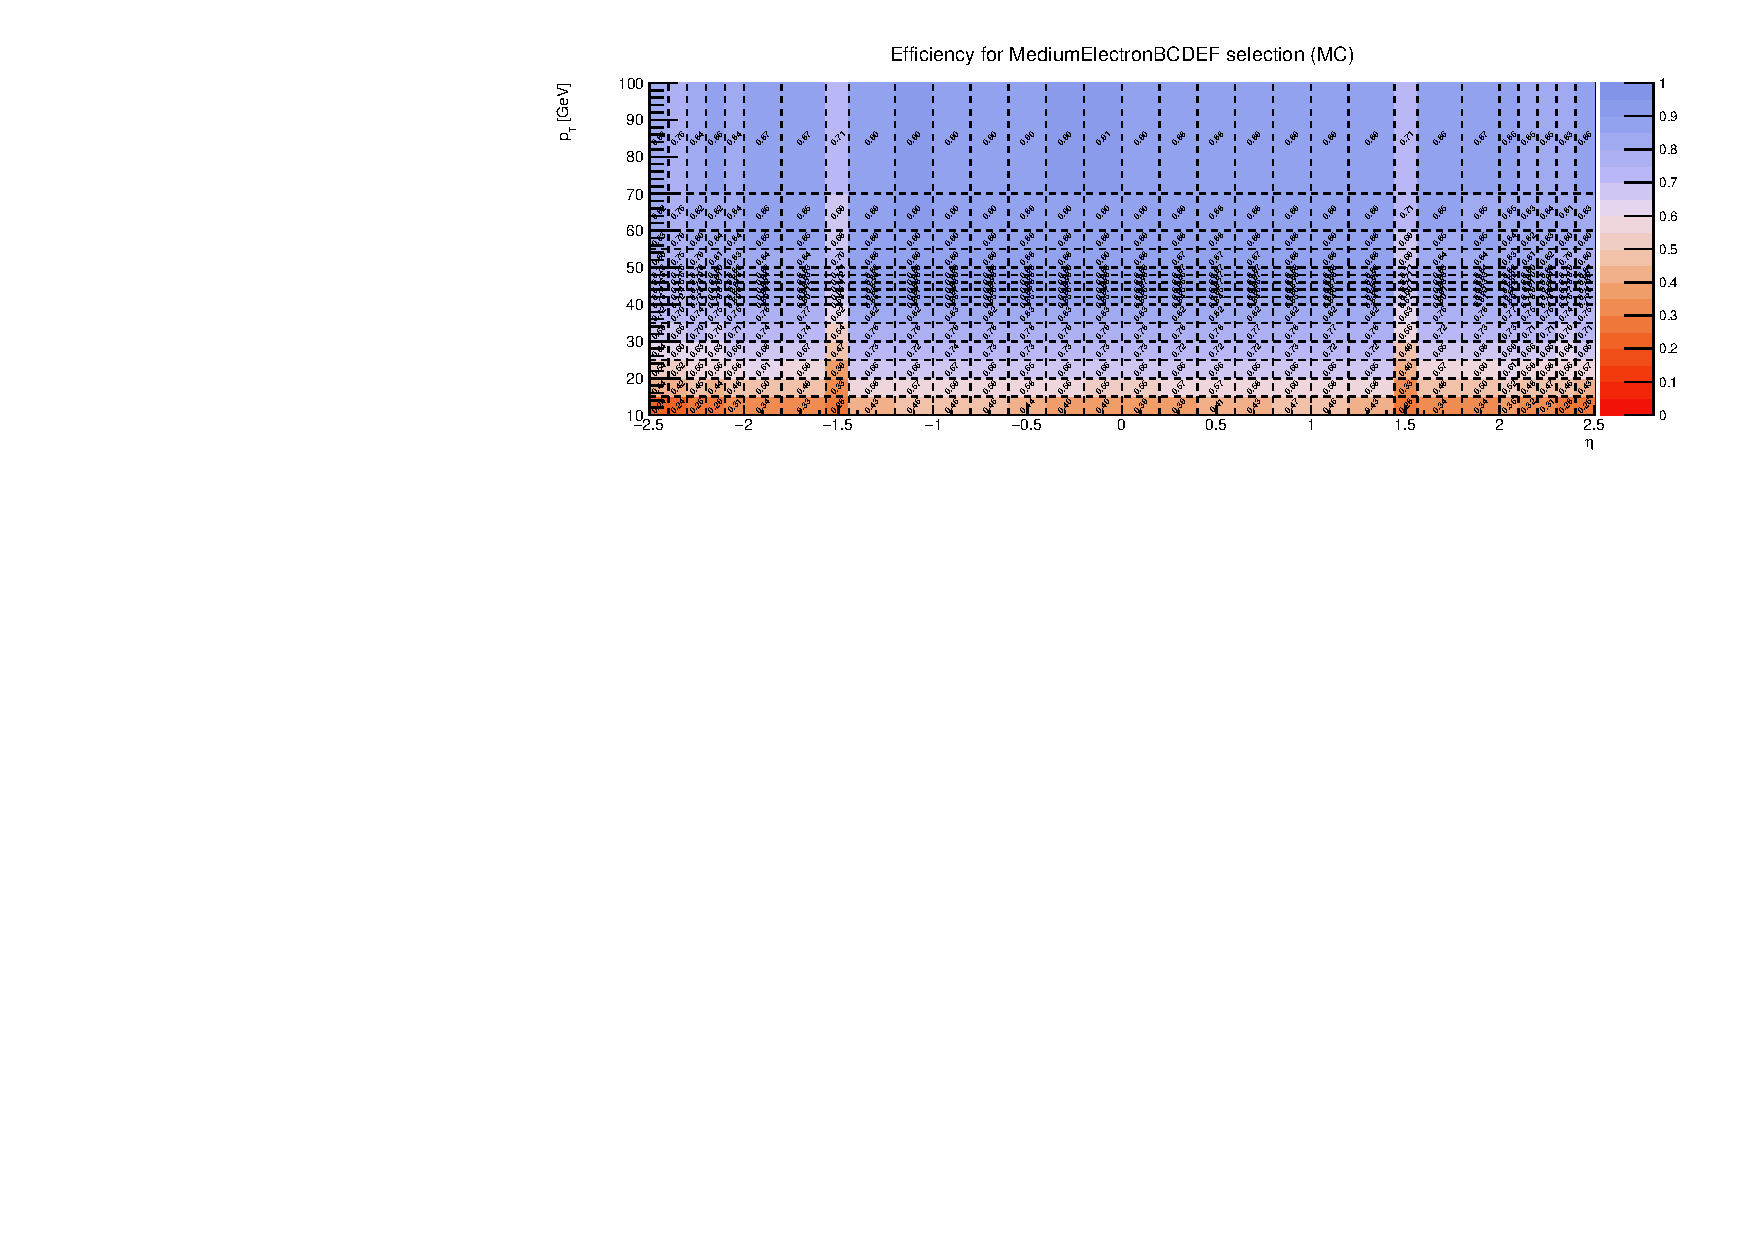
\includegraphics[width=1.00\textwidth]{{figures/eff_mc_MediumElectronBCDEF_0.0-0.0_10.0-100.0}.pdf}
\includegraphics[width=1.00\textwidth]{{figures/eff_mc_MediumElectronGH_0.0-0.0_10.0-100.0}.pdf} 
\caption{Efficiencies extracted from MC for the Medium electron working point after reweighting to the pileup profile in 2016 run eras B to F, and G to H.}
\label{fig:ZeeMCEff}
\end{figure}
\begin{figure}
\centering
\includegraphics[width=1.00\textwidth]{{figures/scalefactors_MediumElectronBCDEF_0.0-0.0_10.0-100.0}.pdf}
\includegraphics[width=1.00\textwidth]{{figures/scalefactors_MediumElectronGH_0.0-0.0_10.0-100.0}.pdf} 
\caption{Scale factors derived from Data/MC efficiencies for the Medium electron working point in 2016 run eras B to F, and G to H.}
\label{fig:ZeeScaleFactors}
\end{figure}
\begin{figure}
\centering
\includegraphics[width=1.00\textwidth]{{figures/scalefactors_MediumElectronBCDEF_statErrorLow_0.0-0.0_10.0-100.0}.pdf}
\includegraphics[width=1.00\textwidth]{{figures/scalefactors_MediumElectronGH_statErrorLow_0.0-0.0_10.0-100.0}.pdf} 
\caption{Statistical uncertainties on the Medium electron scale factors (negative error) in 2016 run eras B to F, and G to H.}
\label{fig:ZeeScaleFactorsErrorHi}
\end{figure}
\begin{figure}
\centering
\includegraphics[width=1.00\textwidth]{{figures/scalefactors_MediumElectronBCDEF_statErrorHigh_0.0-0.0_10.0-100.0}.pdf}
\includegraphics[width=1.00\textwidth]{{figures/scalefactors_MediumElectronGH_statErrorHigh_0.0-0.0_10.0-100.0}.pdf} 
\caption{Statistical uncertainties on the Medium electron scale factors (positive error) in 2016 run eras B to F, and G to H.}
\label{fig:ZeeScaleFactorsErrorLo}
\end{figure}

\section{Assessment of systematic uncertainty}
\label{sec:tnpsyst}
In this section, we quantify the systematic uncertainty arising from five distinct sources related to our ignorance
of the true signal and background shapes, the generator-related uncertainty, and possible selection bias.
In each case, the absolute difference between two alternative methods is taken as the systematic uncertainty.
\subsection{Background shape modeling}
To quantify the uncertainty in deriving the background shape from the data-driven method,
we use an analytic function as an alternative background shape.
The function chosen is a linear combination of: a decaying exponential to model low-energy fakes,
and a wide Gaussian with exponential tails to represent the peaking structure
sculpted by applying energy cuts to a falling combinatorial background mass distribution.
Previously, an error function multiplied with a decaying exponential was used, but this function
has problems related to fit convergence due to poor parameterization.

Examples of fits for 2016 run eras B to F with the analytic background are shown for dimuons in
Figures ~\ref{fig:ZmmAltBkgFits1} and~\ref{fig:ZmmAltBkgFits2}, 
and for dielectrons in Figures~\ref{fig:ZeeAltBkgFits1} and~\ref{fig:ZeeAltBkgFits2}.
These may be compared with the fits using the data-driven background shape 
in section \ref{sec:tnpfits}.
The difference in the Data/MC scale factors derived using the two methods is taken as a systematic; 
see Figures~\ref{fig:ZmmSystBkgModel} and~\ref{fig:ZeeSystBkgModel}.

\begin{figure}
\centering
\includegraphics[width=0.49\textwidth]{figures/Zmm_RecoTemplate_BkgAnalytic_pass_ptBin0_etaBin1.pdf}
\includegraphics[width=0.49\textwidth]{figures/Zmm_RecoTemplate_BkgAnalytic_fail_ptBin0_etaBin1.pdf}
\includegraphics[width=0.49\textwidth]{figures/Zmm_RecoTemplate_BkgAnalytic_pass_ptBin1_etaBin9.pdf}
\includegraphics[width=0.49\textwidth]{figures/Zmm_RecoTemplate_BkgAnalytic_fail_ptBin1_etaBin9.pdf}
\caption{Efficiency extraction fits for the Medium muon working point using the alternative analytic background shape, at low muon transverse momentum.}
\label{fig:ZmmAltBkgFits1}
\end{figure}

\begin{figure}
\centering
\includegraphics[width=0.49\textwidth]{figures/Zmm_RecoTemplate_BkgAnalytic_pass_ptBin7_etaBin0.pdf}
\includegraphics[width=0.49\textwidth]{figures/Zmm_RecoTemplate_BkgAnalytic_fail_ptBin7_etaBin0.pdf}
\includegraphics[width=0.49\textwidth]{figures/Zmm_RecoTemplate_BkgAnalytic_pass_ptBin10_etaBin6.pdf}
\includegraphics[width=0.49\textwidth]{figures/Zmm_RecoTemplate_BkgAnalytic_fail_ptBin10_etaBin6.pdf}
\caption{Efficiency extraction fits for the Medium muon working point using the alternative analytic background shape, at higher values of muon transverse momentum.}
\label{fig:ZmmAltBkgFits2}
\end{figure}

\begin{figure}
\centering
\includegraphics[width=0.49\textwidth]{figures/Zee_RecoTemplate_BkgAnalytic_pass_ptBin0_etaBin0.pdf}
\includegraphics[width=0.49\textwidth]{figures/Zee_RecoTemplate_BkgAnalytic_fail_ptBin0_etaBin0.pdf}
\includegraphics[width=0.49\textwidth]{figures/Zee_RecoTemplate_BkgAnalytic_pass_ptBin1_etaBin19.pdf}
\includegraphics[width=0.49\textwidth]{figures/Zee_RecoTemplate_BkgAnalytic_fail_ptBin1_etaBin19.pdf}
\caption{Efficiency extraction fits for the Medium electron working point using the alternative analytic background shape, at low electron transverse momentum.}
\label{fig:ZeeAltBkgFits1}
\end{figure}

\begin{figure}
\centering
\includegraphics[width=0.49\textwidth]{figures/Zee_RecoTemplate_BkgAnalytic_pass_ptBin3_etaBin23.pdf}
\includegraphics[width=0.49\textwidth]{figures/Zee_RecoTemplate_BkgAnalytic_fail_ptBin3_etaBin23.pdf}
\includegraphics[width=0.49\textwidth]{figures/Zee_RecoTemplate_BkgAnalytic_pass_ptBin14_etaBin17.pdf}
\includegraphics[width=0.49\textwidth]{figures/Zee_RecoTemplate_BkgAnalytic_fail_ptBin14_etaBin17.pdf}
\caption{Efficiency extraction fits for the Medium electron working point using the alternative analytic background shape, at higher values of electron transverse momentum.}
\label{fig:ZeeAltBkgFits2}
\end{figure}

\begin{figure}
\centering
\includegraphics[width=1.00\textwidth]{{figures/scalefactors_Medium2016MuonBCDEF_AltBkg_0.0-0.0_10.0-120.0}.pdf}
\includegraphics[width=1.00\textwidth]{{figures/scalefactors_Medium2016MuonGH_AltBkg_0.0-0.0_10.0-120.0}.pdf} 
\caption{Systematic uncertainties from choice of background model for the Medium muon scale factors in 2016 run eras B to F (top), and G to H (bottom).}
\label{fig:ZmmSystBkgModel}
\end{figure}

\begin{figure}
\centering
\includegraphics[width=1.00\textwidth]{{figures/scalefactors_MediumElectronBCDEF_AltBkg_0.0-0.0_10.0-100.0}.pdf}
\includegraphics[width=1.00\textwidth]{{figures/scalefactors_MediumElectronGH_AltBkg_0.0-0.0_10.0-100.0}.pdf} 
\caption{Systematic uncertainties from choice of background model for the Medium electron scale factors in 2016 run eras B to F (top), and G to H (bottom).}
\label{fig:ZeeSystBkgModel}
\end{figure}
\clearpage
\subsection{Signal resolution modeling}
We consider the uncertainty from using the simulation of the reconstructed Z resonance signal shape
by convolution with an analytic function more complex than a Gaussian to try to capture more detector resolution effects.
The difference in scale factors derived from the data efficiency extraction fits using the two methods
is taken as the systematic uncertainty due to signal resolution modeling.
The alternative function is a single Gaussian with asymmetric, exponential tails.

Examples of fits for 2016 run eras B to F with the alternative resolution function are shown for dimuons in
Figures ~\ref{fig:ZmmAltSigResFits1} and~\ref{fig:ZmmAltSigResFits2}, 
and for dielectrons in Figures~\ref{fig:ZeeAltSigResFits1} and~\ref{fig:ZeeAltSigResFits2}.
These may be compared with the fits using the nominal resolution function
in section \ref{sec:tnpfits}.
The difference in the Data/MC scale factors derived using the two methods is taken as a systematic; 
see Figures~\ref{fig:ZmmSystSigRes} and~\ref{fig:ZeeSystSigRes}.

\begin{figure}
\centering
\includegraphics[width=0.49\textwidth]{figures/Zmm_ResFunc_BkgLPi_pass_ptBin0_etaBin1.pdf}
\includegraphics[width=0.49\textwidth]{figures/Zmm_ResFunc_BkgLPi_fail_ptBin0_etaBin1.pdf}
\includegraphics[width=0.49\textwidth]{figures/Zmm_ResFunc_BkgLPi_pass_ptBin1_etaBin9.pdf}
\includegraphics[width=0.49\textwidth]{figures/Zmm_ResFunc_BkgLPi_fail_ptBin1_etaBin9.pdf}
\caption{Efficiency extraction fits for the Medium muon working point using the analytic detector resolution function, at low muon transverse momentum.}
\label{fig:ZmmAltSigResFits1}
\end{figure}

\begin{figure}
\centering
\includegraphics[width=0.49\textwidth]{figures/Zmm_ResFunc_BkgLPi_pass_ptBin7_etaBin0.pdf}
\includegraphics[width=0.49\textwidth]{figures/Zmm_ResFunc_BkgLPi_fail_ptBin7_etaBin0.pdf}
\includegraphics[width=0.49\textwidth]{figures/Zmm_ResFunc_BkgLPi_pass_ptBin10_etaBin6.pdf}
\includegraphics[width=0.49\textwidth]{figures/Zmm_ResFunc_BkgLPi_fail_ptBin10_etaBin6.pdf}
\caption{Efficiency extraction fits for the Medium muon working point using the analytic detector resolution function, at higher values of muon transverse momentum.}
\label{fig:ZmmAltSigResFits2}
\end{figure}

\begin{figure}
\centering
\includegraphics[width=0.49\textwidth]{figures/Zee_ResFunc_BkgLPiEMu_pass_ptBin0_etaBin0.pdf}
\includegraphics[width=0.49\textwidth]{figures/Zee_ResFunc_BkgLPiEMu_fail_ptBin0_etaBin0.pdf}
\includegraphics[width=0.49\textwidth]{figures/Zee_ResFunc_BkgLPiEMu_pass_ptBin1_etaBin19.pdf}
\includegraphics[width=0.49\textwidth]{figures/Zee_ResFunc_BkgLPiEMu_fail_ptBin1_etaBin19.pdf}
\caption{Efficiency extraction fits for the Medium electron working point using the analytic detector resolution function, at low electron transverse momentum.}
\label{fig:ZeeAltSigResFits1}
\end{figure}

\begin{figure}
\centering
\includegraphics[width=0.49\textwidth]{figures/Zee_ResFunc_BkgLPiEMu_pass_ptBin3_etaBin23.pdf}
\includegraphics[width=0.49\textwidth]{figures/Zee_ResFunc_BkgLPiEMu_fail_ptBin3_etaBin23.pdf}
\includegraphics[width=0.49\textwidth]{figures/Zee_ResFunc_BkgLPiEMu_pass_ptBin14_etaBin17.pdf}
\includegraphics[width=0.49\textwidth]{figures/Zee_ResFunc_BkgLPiEMu_fail_ptBin14_etaBin17.pdf}
\caption{Efficiency extraction fits for the Medium electron working point using the analytic detector resolution function, at higher values of electron transverse momentum.}
\label{fig:ZeeAltSigResFits2}
\end{figure}

\begin{figure}
\centering
\includegraphics[width=1.00\textwidth]{{figures/scalefactors_Medium2016MuonBCDEF_ResFunc_0.0-0.0_10.0-120.0}.pdf}
\includegraphics[width=1.00\textwidth]{{figures/scalefactors_Medium2016MuonGH_ResFunc_0.0-0.0_10.0-120.0}.pdf} 
\caption{Systematic uncertainties from signal resolution modeling for the Medium muon scale factors in 2016 run eras B to F (top), and G to H (bottom).}
\label{fig:ZmmSystSigRes}
\end{figure}

\begin{figure}
\centering
\includegraphics[width=1.00\textwidth]{{figures/scalefactors_MediumElectronBCDEF_ResFunc_0.0-0.0_10.0-100.0}.pdf}
\includegraphics[width=1.00\textwidth]{{figures/scalefactors_MediumElectronGH_ResFunc_0.0-0.0_10.0-100.0}.pdf} 
\caption{Systematic uncertainties from signal resolution modeling for the Medium electron scale factors in 2016 run eras B to F (top), and G to H (bottom).}
\label{fig:ZeeSystSigRes}
\end{figure}

\clearpage
\subsection{Signal final state radiation modeling}
\textcolor{red}{\bf{WE ARE CURRENTLY REDOING THIS WITH PHOTOS}}

The reconstructed dilepton mass shape has a fat tail on the left side because of the effect of final state radiation (FSR).
In these tail events, at least one of the final state leptons radiates a photon,
reducing the energy of the dilepton system and changing the momentum of the emitting lepton.
It is more prevalent for electrons than for muons since bremsstrahlung is suppressed as the fourth power of lepton mass.

Simulation addresses the phenomenon of FSR well in Z boson reconstruction, but we must assess the uncertainty on
how FSR is modeled in the MC generator, which is only an approximation.
We make the unsupported claim that the generator cannot be more incorrect than treating the final state radiation
of electrons as if they were muons and vice versa.

\begin{figure}
\centering
\includegraphics[width=0.49\textwidth]{figures/genTemplatesPlot.pdf}
\includegraphics[width=0.49\textwidth]{figures/genTemplatesPlot2.pdf}
\caption{Left: Difference between the dimuon and dielectron generator-level mass distribution, compared to the reconstructed dielectron mass distribution. Right: Example of how the FSR tail is wagged up and down for a Z(ee) mass distribution.}
\label{fig:ExampleFsrWagging}
\end{figure}

In order to propagate the effect of incorrect FSR simulation to the data efficiency extraction fits
in each phase space bin, we first observe the generator-level final state
dilepton mass distributions for dielectrons and dimuons.
After normalizing both distributions to 1, the ratio of the dielectron to dimuon mass distribution 
is taken as the "wagging" function:

\begin{align*}
  W(M) = \frac{dN}{dM_{\mathrm{Gen}}(ee)} / \frac{dN}{dM_{\mathrm{Gen}}(\mu\mu)}
\end{align*}

The wagging function $W(M)$ is bounded between 0.5 and 2.
We then multiply and divide the reconstructed, simulated, truth-matched mass distribution
by the wagging function to wag the FSR tail up and down, respectively.
See Figure~\ref{fig:ExampleFsrWagging} for an example of this procedure.

These distributions with the FSR tail wagged up and down are used as alternative signal templates
for the data efficiency extraction fits. Examples for 2016 run eras B to F are shown for dimuons in
Figures ~\ref{fig:ZmmAltSigFSRFits1},~\ref{fig:ZmmAltSigFSRFits2},~\ref{fig:ZmmAltSigFSRFits3}, and~\ref{fig:ZmmAltSigFSRFits4};
and for dielectrons in Figures~\ref{fig:ZeeAltSigFSRFits1},~\ref{fig:ZeeAltSigFSRFits2},~\ref{fig:ZeeAltSigFSRFits3}, and~\ref{fig:ZeeAltSigFSRFits4}.
These may be compared with the fits using the nominally simulated FSR tail
in section \ref{sec:tnpfits}.
The maximum difference in the Data/MC scale factors from wagging the FSR tail up or down compared to the nominal value
is taken as the symmetric systematic uncertainty due to FSR modeling;
see Figures~\ref{fig:ZmmSystSigFSR} and~\ref{fig:ZeeSystSigFSR}.

\begin{figure}
\centering
\includegraphics[width=0.49\textwidth]{figures/Zmm_WagFsrUp_BkgLPi_pass_ptBin0_etaBin1.pdf}
\includegraphics[width=0.49\textwidth]{figures/Zmm_WagFsrUp_BkgLPi_fail_ptBin0_etaBin1.pdf}
\includegraphics[width=0.49\textwidth]{figures/Zmm_WagFsrUp_BkgLPi_pass_ptBin1_etaBin9.pdf}
\includegraphics[width=0.49\textwidth]{figures/Zmm_WagFsrUp_BkgLPi_fail_ptBin1_etaBin9.pdf}
\caption{Efficiency extraction fits for the Medium muon working point wagging the FSR tail up, at low muon transverse momentum.}
\label{fig:ZmmAltSigFSRFits1}
\end{figure}
\begin{figure}
\centering
\includegraphics[width=0.49\textwidth]{figures/Zmm_WagFsrUp_BkgLPi_pass_ptBin7_etaBin0.pdf}
\includegraphics[width=0.49\textwidth]{figures/Zmm_WagFsrUp_BkgLPi_fail_ptBin7_etaBin0.pdf}
\includegraphics[width=0.49\textwidth]{figures/Zmm_WagFsrUp_BkgLPi_pass_ptBin10_etaBin6.pdf}
\includegraphics[width=0.49\textwidth]{figures/Zmm_WagFsrUp_BkgLPi_fail_ptBin10_etaBin6.pdf}
\caption{Efficiency extraction fits for the Medium muon working point wagging the FSR tail up, at higher values of muon transverse momentum.}
\label{fig:ZmmAltSigFSRFits2}
\end{figure}
\begin{figure}
\centering
\includegraphics[width=0.49\textwidth]{figures/Zmm_WagFsrDown_BkgLPi_pass_ptBin0_etaBin1.pdf}
\includegraphics[width=0.49\textwidth]{figures/Zmm_WagFsrDown_BkgLPi_fail_ptBin0_etaBin1.pdf}
\includegraphics[width=0.49\textwidth]{figures/Zmm_WagFsrDown_BkgLPi_pass_ptBin1_etaBin9.pdf}
\includegraphics[width=0.49\textwidth]{figures/Zmm_WagFsrDown_BkgLPi_fail_ptBin1_etaBin9.pdf}
\caption{Efficiency extraction fits for the Medium muon working point wagging the FSR tail down, at low muon transverse momentum.}
\label{fig:ZmmAltSigFSRFits3}
\end{figure}
\begin{figure}
\centering
\includegraphics[width=0.49\textwidth]{figures/Zmm_WagFsrDown_BkgLPi_pass_ptBin7_etaBin0.pdf}
\includegraphics[width=0.49\textwidth]{figures/Zmm_WagFsrDown_BkgLPi_fail_ptBin7_etaBin0.pdf}
\includegraphics[width=0.49\textwidth]{figures/Zmm_WagFsrDown_BkgLPi_pass_ptBin10_etaBin6.pdf}
\includegraphics[width=0.49\textwidth]{figures/Zmm_WagFsrDown_BkgLPi_fail_ptBin10_etaBin6.pdf}
\caption{Efficiency extraction fits for the Medium muon working point wagging the FSR tail down, at higher values of muon transverse momentum.}
\label{fig:ZmmAltSigFSRFits4}
\end{figure}

\begin{figure}
\centering
\includegraphics[width=0.49\textwidth]{figures/Zee_WagFsrUp_BkgLPiEMu_pass_ptBin0_etaBin0.pdf}
\includegraphics[width=0.49\textwidth]{figures/Zee_WagFsrUp_BkgLPiEMu_fail_ptBin0_etaBin0.pdf}
\includegraphics[width=0.49\textwidth]{figures/Zee_WagFsrUp_BkgLPiEMu_pass_ptBin1_etaBin19.pdf}
\includegraphics[width=0.49\textwidth]{figures/Zee_WagFsrUp_BkgLPiEMu_fail_ptBin1_etaBin19.pdf}
\caption{Efficiency extraction fits for the Medium electron working point wagging the FSR tail up, at low electron transverse momentum.}
\label{fig:ZeeAltSigFSRFits1}
\end{figure}
\begin{figure}
\centering
\includegraphics[width=0.49\textwidth]{figures/Zee_WagFsrUp_BkgLPiEMu_pass_ptBin3_etaBin23.pdf}
\includegraphics[width=0.49\textwidth]{figures/Zee_WagFsrUp_BkgLPiEMu_fail_ptBin3_etaBin23.pdf}
\includegraphics[width=0.49\textwidth]{figures/Zee_WagFsrUp_BkgLPiEMu_pass_ptBin14_etaBin17.pdf}
\includegraphics[width=0.49\textwidth]{figures/Zee_WagFsrUp_BkgLPiEMu_fail_ptBin14_etaBin17.pdf}
\caption{Efficiency extraction fits for the Medium electron working point wagging the FSR tail up, at higher values of electron transverse momentum.}
\label{fig:ZeeAltSigFSRFits2}
\end{figure}
\begin{figure}
\centering
\includegraphics[width=0.49\textwidth]{figures/Zee_WagFsrDown_BkgLPiEMu_pass_ptBin0_etaBin0.pdf}
\includegraphics[width=0.49\textwidth]{figures/Zee_WagFsrDown_BkgLPiEMu_fail_ptBin0_etaBin0.pdf}
\includegraphics[width=0.49\textwidth]{figures/Zee_WagFsrDown_BkgLPiEMu_pass_ptBin1_etaBin19.pdf}
\includegraphics[width=0.49\textwidth]{figures/Zee_WagFsrDown_BkgLPiEMu_fail_ptBin1_etaBin19.pdf}
\caption{Efficiency extraction fits for the Medium electron working point wagging the FSR tail down, at low electron transverse momentum.}
\label{fig:ZeeAltSigFSRFits3}
\end{figure}

\begin{figure}
\centering
\includegraphics[width=0.49\textwidth]{figures/Zee_WagFsrDown_BkgLPiEMu_pass_ptBin3_etaBin23.pdf}
\includegraphics[width=0.49\textwidth]{figures/Zee_WagFsrDown_BkgLPiEMu_fail_ptBin3_etaBin23.pdf}
\includegraphics[width=0.49\textwidth]{figures/Zee_WagFsrDown_BkgLPiEMu_pass_ptBin14_etaBin17.pdf}
\includegraphics[width=0.49\textwidth]{figures/Zee_WagFsrDown_BkgLPiEMu_fail_ptBin14_etaBin17.pdf}
\caption{Efficiency extraction fits for the Medium electron working point wagging the FSR tail down, at higher values of electron transverse momentum.}
\label{fig:ZeeAltSigFSRFits4}
\end{figure}

\begin{figure}
\centering
\includegraphics[width=1.00\textwidth]{{figures/scalefactors_Medium2016MuonBCDEF_FsrModeling_0.0-0.0_10.0-120.0}.pdf}
\includegraphics[width=1.00\textwidth]{{figures/scalefactors_Medium2016MuonGH_FsrModeling_0.0-0.0_10.0-120.0}.pdf} 
\caption{Systematic uncertainties from signal FSR modeling for the Medium muon scale factors in 2016 run eras B to F (top), and G to H (bottom).}
\label{fig:ZmmSystSigFSR}
\end{figure}
\begin{figure}
\centering
\includegraphics[width=1.00\textwidth]{{figures/scalefactors_MediumElectronBCDEF_FsrModeling_0.0-0.0_10.0-100.0}.pdf}
\includegraphics[width=1.00\textwidth]{{figures/scalefactors_MediumElectronGH_FsrModeling_0.0-0.0_10.0-100.0}.pdf} 
\caption{Systematic uncertainties from signal FSR modeling for the Medium electron scale factors in 2016 run eras B to F (top), and G to H (bottom).}
\label{fig:ZeeSystSigFSR}
\end{figure}
\clearpage
\subsection{Choice of generator}
The choice of generator used to determine the MC can affect the scale factor determination.
The differences in generator implementations, including leading-order versus next-to-leading order simulation,
can affect the fraction of passing and failing probes, and the truth-matching efficiency.
Therefore we use a different implementation (\textsc{MadGraph5} at leading-order)
instead of the nominal (\textsc{MadGraph5\_aMC@NLO}) to determine the MC efficiency and the signal PDF,
and take the size of the change in the scale factors as the symmetric systematic uncertainty
from the choice of generator.
See Figures~\ref{fig:ZmmSystMCGen} and~\ref{fig:ZeeSystMCGen}.

\begin{figure}
\centering
\includegraphics[width=1.00\textwidth]{{figures/scalefactors_Medium2016MuonBCDEF_AltGen_0.0-0.0_10.0-120.0}.pdf}
\includegraphics[width=1.00\textwidth]{{figures/scalefactors_Medium2016MuonGH_AltGen_0.0-0.0_10.0-120.0}.pdf} 
\caption{Systematic uncertainties from generator choice for the Medium muon scale factors in 2016 run eras B to F (top), and G to H (bottom).}
\label{fig:ZmmSystMCGen}
\end{figure}

\begin{figure}
\centering
\includegraphics[width=1.00\textwidth]{{figures/scalefactors_MediumElectronBCDEF_AltGen_0.0-0.0_10.0-100.0}.pdf}
\includegraphics[width=1.00\textwidth]{{figures/scalefactors_MediumElectronGH_AltGen_0.0-0.0_10.0-100.0}.pdf} 
\caption{Systematic uncertainties from generator choice for the Medium electron scale factors in 2016 run eras B to F (top), and G to H (bottom).}
\label{fig:ZeeSystMCGen}
\end{figure}
\clearpage
\subsection{Bias from choice of tag selection}
The choice of tag selection cuts is motivated by the realities of the experiment, such as
detector acceptance and trigger $p_{T}$ thresholds. The tag selection can bias the data efficiency,
so we account for this by observing the change in the Data/MC scale factors when the 
tag selection is changed. The alternative tag selection has a $p_{T}$ threshold 5 $\GeV$ higher, and 
uses the Medium working point for identification and isolation.

Examples of fits for 2016 run eras B to F with the alternative tag selection applied to Data and MC are shown for dimuons in
Figures ~\ref{fig:ZmmAltAltTagFits1} and~\ref{fig:ZmmAltAltTagFits2}, 
and for dielectrons in Figures~\ref{fig:ZeeAltAltTagFits1} and~\ref{fig:ZeeAltAltTagFits2}.
These may be compared with the fits using the nominal tag selection in section \ref{sec:tnpfits}.
The difference in the Data/MC scale factors derived using the two methods is taken as a systematic; 
see Figures~\ref{fig:ZmmSystAltTag} and~\ref{fig:ZeeSystAltTag}.

\begin{figure}
\centering
\includegraphics[width=0.49\textwidth]{figures/Zmm_AltTag_pass_ptBin0_etaBin1.pdf}
\includegraphics[width=0.49\textwidth]{figures/Zmm_AltTag_fail_ptBin0_etaBin1.pdf}
\includegraphics[width=0.49\textwidth]{figures/Zmm_AltTag_pass_ptBin1_etaBin9.pdf}
\includegraphics[width=0.49\textwidth]{figures/Zmm_AltTag_fail_ptBin1_etaBin9.pdf}
\caption{Efficiency extraction fits for the Medium muon working point using the alternative tag selection, at low muon transverse momentum.}
\label{fig:ZmmAltAltTagFits1}
\end{figure}

\begin{figure}
\centering
\includegraphics[width=0.49\textwidth]{figures/Zmm_AltTag_pass_ptBin7_etaBin0.pdf}
\includegraphics[width=0.49\textwidth]{figures/Zmm_AltTag_fail_ptBin7_etaBin0.pdf}
\includegraphics[width=0.49\textwidth]{figures/Zmm_AltTag_pass_ptBin10_etaBin6.pdf}
\includegraphics[width=0.49\textwidth]{figures/Zmm_AltTag_fail_ptBin10_etaBin6.pdf}
\caption{Efficiency extraction fits for the Medium muon working point using the alternative tag selection, at higher values of muon transverse momentum.}
\label{fig:ZmmAltAltTagFits2}
\end{figure}

\begin{figure}
\centering
\includegraphics[width=0.49\textwidth]{figures/Zee_AltTag_pass_ptBin0_etaBin0.pdf}
\includegraphics[width=0.49\textwidth]{figures/Zee_AltTag_fail_ptBin0_etaBin0.pdf}
\includegraphics[width=0.49\textwidth]{figures/Zee_AltTag_pass_ptBin1_etaBin19.pdf}
\includegraphics[width=0.49\textwidth]{figures/Zee_AltTag_fail_ptBin1_etaBin19.pdf}
\caption{Efficiency extraction fits for the Medium electron working point using the alternative tag selection, at low electron transverse momentum.}
\label{fig:ZeeAltAltTagFits1}
\end{figure}

\begin{figure}
\centering
\includegraphics[width=0.49\textwidth]{figures/Zee_AltTag_pass_ptBin3_etaBin23.pdf}
\includegraphics[width=0.49\textwidth]{figures/Zee_AltTag_fail_ptBin3_etaBin23.pdf}
\includegraphics[width=0.49\textwidth]{figures/Zee_AltTag_pass_ptBin14_etaBin17.pdf}
\includegraphics[width=0.49\textwidth]{figures/Zee_AltTag_fail_ptBin14_etaBin17.pdf}
\caption{Efficiency extraction fits for the Medium electron working point using the alternative tag selection, at higher values of electron transverse momentum.}
\label{fig:ZeeAltAltTagFits2}
\end{figure}

\begin{figure}
\centering
\includegraphics[width=1.00\textwidth]{{figures/scalefactors_Medium2016MuonBCDEF_AltTag_0.0-0.0_10.0-120.0}.pdf}
\includegraphics[width=1.00\textwidth]{{figures/scalefactors_Medium2016MuonGH_AltTag_0.0-0.0_10.0-120.0}.pdf} 
\caption{Systematic uncertainties from choice of tag selection for the Medium muon scale factors in 2016 run eras B to F (top), and G to H (bottom).}
\label{fig:ZmmSystAltTag}
\end{figure}

\begin{figure}
\centering
\includegraphics[width=1.00\textwidth]{{figures/scalefactors_MediumElectronBCDEF_AltTag_0.0-0.0_10.0-100.0}.pdf}
\includegraphics[width=1.00\textwidth]{{figures/scalefactors_MediumElectronGH_AltTag_0.0-0.0_10.0-100.0}.pdf} 
\caption{Systematic uncertainties from choice of tag selection for the Medium electron scale factors in 2016 run eras B to F (top), and G to H (bottom).}
\label{fig:ZeeSystAltTag}
\end{figure}
\clearpage
\subsection{Total impact of systematic uncertainties}
The percent impacts of each source of uncertainty on the inclusive Z(ll) cross section
are shown in Table~\ref{tab:ZYieldImpacts}.
This uncertainty essentially defines the sensitivity of the momentum spectra measurement.
On the other hand, for the dark matter search against the diboson final states, it is nearly irrelevant.
There, it is sufficient to apply a flat uncertainty of this size, independent of kinematics.

\begin{table}[htbp]
  \begin{center}
 {\small
  \begin{tabular} {lrr}
\hline
  \multirow{2}{*}{Source of Uncertainty} & Z(ee) Yield& Z($\mu\mu$) Yield \\
                                         & \% Impact  & \% Impact         \\
  \hline
  Background shape                       & 0.58       & 0.61              \\
  Signal resolution                      & 0.06       & 0.32              \\
  Signal FSR model                       & 0.80       & 0.48              \\
  Generator choice                       & 0.88       & 0.31              \\
  Tag selection                          & 0.51       & 0.32              \\
  \hline                                                           
  Total scale factor impact              & 1.4        & 0.95              \\
  \hline
  \end{tabular}
}
  \caption{Impact of the scale factor uncertainties on the inclusive cross section.}
  \label{tab:ZYieldImpacts}
  \end{center}
\end{table}




\chapter{Diboson studies}
\label{chap:dibosons}

The resonant diboson processes $\Z\Z$ and $\W\Z$ are an irreducible background of the
dark matter searches involving any Z boson in the final state.
In final states with little hadronic activity e.g. this work, 
the other background processes which contribute substantially are easy to reject and pare down.
Then, the diboson becomes the main problem due to our limited theoretical understanding, and nothing beside remains.

Below, I survey the current status of theoretical calculations for dibosons. 
Then, I discuss a strategy which makes use of independent control samples from the experimental data,
to improve upon inaccuracies arising from those calculations.

\section{Limitations of simulating diboson processes}

All simulated physics processes in this work are susceptible to uncertainties due to: the proton parton distribution functions; the QCD scale, $\alpha_s$; and the renormalization and factorization scales in the quantum field theory.
Consistent with the other processes, these effects are propagated to both the overall cross sections and the transverse momentum spectra of the $\Z\Z$ and $\W\Z$ processes.
The details of this propagation are described later, in section ??.
For the purposes of motivating this chapter, it suffices to say that the effect of these is roughly 10\%. 

Meanwhile, as previously outlined in \ref{sec:higher-order-corrections}, the endgame-level precision for the $\Z\Z$ and $\W\Z$ simulations is NNLO in QCD and NLO in electroweak.
Since no cohesive theoretical calculation is available at this level of precision, our duct-tape assembly of higher-order corrections come at a price.
Namely, we do not count the contribution from diagrams at NLO in both QCD and electroweak. Thus arises the so-called "QCD-electroweak cross-term."

The overall electroweak NLO correction to the $\W\Z$ process is relatively small, since the virtual corrections and photon-induced corrections partially cancel.
Therefore, the NLO QCD-electroweak cross-term for the $\W\Z$ process is also small.
On the other hand, the electroweak NLO corrections to the $\Z\Z$ process are large and momentum-dependent.
They bring a 10\% net reduction of the overall $\Z\Z$ yield, with a strong dependence on the lesser boson $p_T$.
The $\met$ spectrum becomes much softer, with a correction of around $-40\%$ at lesser Z boson $p_T$ of $700 \GeV$.
For this reason, we cannot neglect the QCD-electroweak cross term for the $\Z\Z$ process, and a conservative
assessment of this missing term gives an overall effect of roughly $25\%$.

Yet another conservative step is taken regarding the NNLO QCD corrections.
For lack of a better method, we carry forward the PDF and QCD scale uncertainties from the original POWHEG calculation at NLO in QCD,
even though the final distributions are corrected to NNLO in QCD.
This represents another setback in our understanding of the diboson processes.

So far, in this chapter I have presented a bleak picture of the diboson calculations.
There is a silver lining to this: it is possible to control these cumbersome uncertainties by exploring the experimental data.
The name of the game is to extrapolate from diboson events with fully visible decays, to the transverse momentum spectrum of diboson processes with substantial missing energy. 
The sections below outline the statistically independent control samples, in which are gathered these aforementioned visible diboson decays.

\section{Three-lepton control sample}
\label{sec:wz3l}
The $\WZ$ process is estimated from events with three well-reconstructed leptons and a nominal amount of $\met$.

Events must have exactly two opposite-charged electrons/muons with $\pt > 25/20~\GeV$ each.
The mass of this dilepton system ($\mll$) is required to be $\left|\mll-m_{\Z}\right| < 15\GeV$, consistent with the decay of a $\Z$ boson.
An additional well-identified electron or muon is required, representing the W boson.
To enhance the purity of the $\WZ$ selection, $\met$ of at least 30\GeV is required,
the invariant mass of all three leptons $m_{3\Lep}$ is required to be larger than $100\GeV$,
and the invariant mass between all opposite sign-same flavour lepton pairs ($m_{2\Lep}$) is required to be larger than $4\GeV$.
These requirements follow the procedure used in the CMS measurement of the $\WZ$ production cross-section~\cite{Khachatryan:2016tgp}.

Since there is no danger of contamination, no veto on additional hadronically-decaying $\tau$ leptons is applied.
A relaxed b-jet veto is applied which rejects events where a jet passes the most stringent b-jet identification requirement.

\section{Four-lepton control sample}
\label{sec:zz4l}
The $\ZZ$ process is estimated from events with four well-reconstructed leptons.
In addition to a stringently-identified $\Z$ candidate as in Section~\ref{sec:wz3l}, 
a second candidate is required, whose decay products only need to pass loose identification requirement.
This choice reflects the very high purity of the four-lepton selection. 
For both candidates, the $\Z$ mass requirement is enforced.

Again as in Section~\ref{sec:wz3l}, there is no hadronic $\tau$ veto, and a relaxed b-jet veto is applied.

\section{Emulation of the missing energy}
\label{sec:fakemet}
We now seek to solve the aforementioned problem. 
Using the pure control samples with three or four leptons, the aim is to extrapolate
to an estimation of the missing energy spectra for $\Z\Z$ and $\W\Z$ events 
with only two reconstructed leptons and missing energy in the final state.
The $\W\Z$ process can appear this way due to a lost lepton.
A lepton can be lost due to inefficiency in the reconstruction and identification of leptons, or otherwise the limited detector acceptance.

We extrapolate to the $2\ell+\met$ final state by furnishing a quantity known as the emulated $\met$ or so-called ``fake $\met$.''
For the $\WZ$ process, the fake $\met$ is the true $\W$ boson $\pt$.
It is estimated by calculating the vectorial sum of the $\met$ vector and the transverse momentum vector of the third lepton.
For the $\Z\Z$ process, the fake $\met$ comes from taking the sum of any nominal true $\met$ and one of the leptonically-decaying $\Z$ bosons.
The $\Z$ boson which is made to vanish in this disappearing act is chosen to be the one whose reconstructed invariant mass is further from the
nominal $\Z$ mass of $91.1876 \GeV$.
\footnote{The choice of which $\Z$ candidate to use for the emulation of the $\met$ is arbitrary and has almost no effect on the resulting distribution.}.

The resulting emulated \met spectra are shown in Fig.~\ref{fig:histo_fakemet}.

\begin{figure}[htbp]
\centering
\includegraphics[width=0.48\textwidth]{figures/wz_fakemet_allcuts_postfit.pdf}
\includegraphics[width=0.48\textwidth]{figures/zz_fakemet_allcuts_postfit.pdf}
\includegraphics[width=0.48\textwidth]{figures/ratio_zzvswz.pdf}
\caption{Emulated $\met$
distribution for  the $\W\Z \to 3\Lep\nu$(top left) and $\Z\Z \to 4\Lep$ (top right)
control regions, and the ratio between both distributions in data and simulation (bottom).
 Uncertainty bands correspond to both statistical and systematic uncertainty.}
\label{fig:histo_fakemet}
\end{figure}



%%% This is an example first chapter.  You should put chapter/appendix that you
%% write into a separate file, and add a line \include{yourfilename} to
%% main.tex, where `yourfilename.tex' is the name of the chapter/appendix file.
%% You can process specific files by typing their names in at the 
%% \files=
%% prompt when you run the file main.tex through LaTeX.
\chapter{Introduction}

Micro-optimization is a technique to reduce the overall operation count of
floating point operations.  In a standard floating point unit, floating
point operations are fairly high level, such as ``multiply'' and ``add'';
in a micro floating point unit ($\mu$FPU), these have been broken down into
their constituent low-level floating point operations on the mantissas and
exponents of the floating point numbers.

Chapter two describes the architecture of the $\mu$FPU unit, and the
motivations for the design decisions made.

Chapter three describes the design of the compiler, as well as how the
optimizations discussed in section~\ref{ch1:opts} were implemented.

Chapter four describes the purpose of test code that was compiled, and which
statistics were gathered by running it through the simulator.  The purpose
is to measure what effect the micro-optimizations had, compared to
unoptimized code.  Possible future expansions to the project are also
discussed.

\section{Motivations for micro-optimization}

The idea of micro-optimization is motivated by the recent trends in computer
architecture towards low-level parallelism and small, pipelineable
instruction sets \cite{patterson:risc,rad83}.  By getting rid of more
complex instructions and concentrating on optimizing frequently used
instructions, substantial increases in performance were realized.

Another important motivation was the trend towards placing more of the
burden of performance on the compiler.  Many of the new architectures depend
on an intelligent, optimizing compiler in order to realize anywhere near
their peak performance
\cite{ellis:bulldog,pet87,coutant:precision-compilers}.  In these cases, the
compiler not only is responsible for faithfully generating native code to
match the source language, but also must be aware of instruction latencies,
delayed branches, pipeline stages, and a multitude of other factors in order
to generate fast code \cite{gib86}.

Taking these ideas one step further, it seems that the floating point
operations that are normally single, large instructions can be further broken
down into smaller, simpler, faster instructions, with more control in the
compiler and less in the hardware.  This is the idea behind a
micro-optimizing FPU; break the floating point instructions down into their
basic components and use a small, fast implementation, with a large part of
the burden of hardware allocation and optimization shifted towards
compile-time.

Along with the hardware speedups possible by using a $\mu$FPU, there are
also optimizations that the compiler can perform on the code that is
generated.  In a normal sequence of floating point operations, there are
many hidden redundancies that can be eliminated by allowing the compiler to
control the floating point operations down to their lowest level.  These
optimizations are described in detail in section~\ref{ch1:opts}.

\section{Description of micro-optimization}\label{ch1:opts}

In order to perform a sequence of floating point operations, a normal FPU
performs many redundant internal shifts and normalizations in the process of
performing a sequence of operations.  However, if a compiler can
decompose the floating point operations it needs down to the lowest level,
it then can optimize away many of these redundant operations.  

If there is some additional hardware support specifically for
micro-optimization, there are additional optimizations that can be
performed.  This hardware support entails extra ``guard bits'' on the
standard floating point formats, to allow several unnormalized operations to
be performed in a row without the loss information\footnote{A description of
the floating point format used is shown in figures~\ref{exponent-format}
and~\ref{mantissa-format}.}.  A discussion of the mathematics behind
unnormalized arithmetic is in appendix~\ref{unnorm-math}.

The optimizations that the compiler can perform fall into several categories:

\subsection{Post Multiply Normalization}

When more than two multiplications are performed in a row, the intermediate
normalization of the results between multiplications can be eliminated.
This is because with each multiplication, the mantissa can become
denormalized by at most one bit.  If there are guard bits on the mantissas
to prevent bits from ``falling off'' the end during multiplications, the
normalization can be postponed until after a sequence of several
multiplies\footnote{Using unnormalized numbers for math is not a new idea; a
good example of it is the Control Data CDC 6600, designed by Seymour Cray.
\cite{thornton:cdc6600} The CDC 6600 had all of its instructions performing
unnormalized arithmetic, with a separate {\tt NORMALIZE} instruction.}.

% This is an example of how you would use tgrind to include an example
% of source code; it is commented out in this template since the code
% example file does not exist.  To use it, you need to remove the '%' on the
% beginning of the line, and insert your own information in the call.
%
%\tagrind[htbp]{code/pmn.s.tex}{Post Multiply Normalization}{opt:pmn}

As you can see, the intermediate results can be multiplied together, with no
need for intermediate normalizations due to the guard bit.  It is only at
the end of the operation that the normalization must be performed, in order
to get it into a format suitable for storing in memory\footnote{Note that
for purposed of clarity, the pipeline delays were considered to be 0, and
the branches were not delayed.}.

\subsection{Block Exponent}

In a unoptimized sequence of additions, the sequence of operations is as
follows for each pair of numbers ($m_1$,$e_1$) and ($m_2$,$e_2$).
\begin{enumerate}
  \item Compare $e_1$ and $e_2$.
  \item Shift the mantissa associated with the smaller exponent $|e_1-e_2|$
        places to the right.
  \item Add $m_1$ and $m_2$.
  \item Find the first one in the resulting mantissa.
  \item Shift the resulting mantissa so that normalized
  \item Adjust the exponent accordingly.
\end{enumerate}

Out of 6 steps, only one is the actual addition, and the rest are involved
in aligning the mantissas prior to the add, and then normalizing the result
afterward.  In the block exponent optimization, the largest mantissa is
found to start with, and all the mantissa's shifted before any additions
take place.  Once the mantissas have been shifted, the additions can take
place one after another\footnote{This requires that for n consecutive
additions, there are $\log_{2}n$ high guard bits to prevent overflow.  In
the $\mu$FPU, there are 3 guard bits, making up to 8 consecutive additions
possible.}.  An example of the Block Exponent optimization on the expression
X = A + B + C is given in figure~\ref{opt:be}.

% This is an example of how you would use tgrind to include an example
% of source code; it is commented out in this template since the code
% example file does not exist.  To use it, you need to remove the '%' on the
% beginning of the line, and insert your own information in the call.
%
%\tgrind[htbp]{code/be.s.tex}{Block Exponent}{opt:be}

\section{Integer optimizations}

As well as the floating point optimizations described above, there are
also integer optimizations that can be used in the $\mu$FPU.  In concert
with the floating point optimizations, these can provide a significant
speedup.  

\subsection{Conversion to fixed point}

Integer operations are much faster than floating point operations; if it is
possible to replace floating point operations with fixed point operations,
this would provide a significant increase in speed.

This conversion can either take place automatically or or based on a
specific request from the programmer.  To do this automatically, the
compiler must either be very smart, or play fast and loose with the accuracy
and precision of the programmer's variables.  To be ``smart'', the computer
must track the ranges of all the floating point variables through the
program, and then see if there are any potential candidates for conversion
to floating point.  This technique is discussed further in
section~\ref{range-tracking}, where it was implemented.

The other way to do this is to rely on specific hints from the programmer
that a certain value will only assume a specific range, and that only a
specific precision is desired.  This is somewhat more taxing on the
programmer, in that he has to know the ranges that his values will take at
declaration time (something normally abstracted away), but it does provide
the opportunity for fine-tuning already working code.

Potential applications of this would be simulation programs, where the
variable represents some physical quantity; the constraints of the physical
system may provide bounds on the range the variable can take.
\subsection{Small Constant Multiplications}

One other class of optimizations that can be done is to replace
multiplications by small integer constants into some combination of
additions and shifts.  Addition and shifting can be significantly faster
than multiplication.  This is done by using some combination of
\begin{eqnarray*}
a_i & = & a_j + a_k \\
a_i & = & 2a_j + a_k \\
a_i & = & 4a_j + a_k \\
a_i & = & 8a_j + a_k \\
a_i & = & a_j - a_k \\
a_i & = & a_j \ll m \mbox{shift}
\end{eqnarray*}
instead of the multiplication.  For example, to multiply $s$ by 10 and store
the result in $r$, you could use:
\begin{eqnarray*}
r & = & 4s + s\\
r & = & r + r
\end{eqnarray*}
Or by 59:
\begin{eqnarray*}
t & = & 2s + s \\
r & = & 2t + s \\
r & = & 8r + t
\end{eqnarray*}
Similar combinations can be found for almost all of the smaller
integers\footnote{This optimization is only an ``optimization'', of course,
when the amount of time spent on the shifts and adds is less than the time
that would be spent doing the multiplication.  Since the time costs of these
operations are known to the compiler in order for it to do scheduling, it is
easy for the compiler to determine when this optimization is worth using.}.
\cite{magenheimer:precision}

\section{Other optimizations}

\subsection{Low-level parallelism}

The current trend is towards duplicating hardware at the lowest level to
provide parallelism\footnote{This can been seen in the i860; floating point
additions and multiplications can proceed at the same time, and the RISC
core be moving data in and out of the floating point registers and providing
flow control at the same time the floating point units are active. \cite{byte:i860}}

Conceptually, it is easy to take advantage to low-level parallelism in the
instruction stream by simply adding more functional units to the $\mu$FPU,
widening the instruction word to control them, and then scheduling as many
operations to take place at one time as possible.

However, simply adding more functional units can only be done so many times;
there is only a limited amount of parallelism directly available in the
instruction stream, and without it, much of the extra resources will go to
waste.  One process used to make more instructions potentially schedulable
at any given time is ``trace scheduling''.  This technique originated in the
Bulldog compiler for the original VLIW machine, the ELI-512.
\cite{ellis:bulldog,colwell:vliw}  In trace scheduling, code can be
scheduled through many basic blocks at one time, following a single
potential ``trace'' of program execution.  In this way, instructions that
{\em might\/} be executed depending on a conditional branch further down in
the instruction stream are scheduled, allowing an increase in the potential
parallelism.  To account for the cases where the expected branch wasn't
taken, correction code is inserted after the branches to undo the effects of
any prematurely executed instructions.

\subsection{Pipeline optimizations}

In addition to having operations going on in parallel across functional
units, it is also typical to have several operations in various stages of
completion in each unit.  This pipelining allows the throughput of the
functional units to be increased, with no increase in latency.

There are several ways pipelined operations can be optimized.  On the
hardware side, support can be added to allow data to be recirculated back
into the beginning of the pipeline from the end, saving a trip through the
registers.  On the software side, the compiler can utilize several tricks to
try to fill up as many of the pipeline delay slots as possible, as
seendescribed by Gibbons. \cite{gib86}



%\include{chap2}
%\section{Preamble}\label{sec:preamble}
%\section{Reconstructing proton-proton collision with the CMS detector}\label{sec:detector}
%\section{Data samples}\label{sec:samples}
%\section{Efficiency of lepton trigger, reconstruction, and identification}\label{sec:lepeff}
%\section{Diboson and nonresonant background control samples}\label{sec:dmbkg}
%\section{Search for dark matter in events with high missing transverse energy}\label{sec:zlldm}
%\section{Z boson transverse momentum spectrum, charged lepton decay mode}\label{sec:zllpt}
%\section{Z boson transverse momentum spectrum, neutrino decay mode}\label{sec:zvvpt}
%\section{Combined measurement of the Z boson transverse momentum spectrum}\label{sec:zptcombo}
\appendix
\chapter{Tables}

\begin{table}
\caption{Armadillos}
\label{arm:table}
\begin{center}
\begin{tabular}{||l|l||}\hline
Armadillos & are \\\hline
our	   & friends \\\hline
\end{tabular}
\end{center}
\end{table}

\clearpage
\newpage

\chapter{Figures}

\vspace*{-3in}

\begin{figure}
\vspace{2.4in}
\caption{Armadillo slaying lawyer.}
\label{arm:fig1}
\end{figure}
\clearpage
\newpage

\begin{figure}
\vspace{2.4in}
\caption{Armadillo eradicating national debt.}
\label{arm:fig2}
\end{figure}
\clearpage
\newpage

%% This defines the bibliography file (main.bib) and the bibliography style.
%% If you want to create a bibliography file by hand, change the contents of
%% this file to a `thebibliography' environment.  For more information 
%% see section 4.3 of the LaTeX manual.
\begin{singlespace}
\bibliography{main}
%\bibliographystyle{plain}
%\bibliographystyle{ieeetr}
\bibliographystyle{unsrt}
\end{singlespace}

\end{document}

